\documentclass[nobib,notoc,twoside,symmetric]{tufte-book}
\setcounter{tocdepth}{4}
\setcounter{secnumdepth}{4}

\usepackage{marginfix}
%to fix margins
\usepackage{multicol}
%for two-column.
\usepackage{CJKutf8}
%for mandarin

%\usepackage{scrextend} 
%\changefontsizes[11pt]{12pt}

\renewcommand{\footnotesize}{\small}

\geometry{a4paper,landscape,inner=30mm,top=15mm,bottom=10mm,headsep=\baselineskip,textwidth=170mm,marginparsep=8mm,marginparwidth=80mm,textheight=170mm,headheight=\baselineskip}

%\geometry{showframe}% for debugging purposes -- displays the margins

%\usepackage{stmaryrd}
%\usepackage{fontawesome}

\usepackage{amsmath,amsthm,amssymb,amsfonts}
\theoremstyle{definition}
\newtheorem{theorem}{Theorem}[section]
\newtheorem*{theorem*}{Theorem}
\newtheorem{corollary}[theorem]{Corollary}
\newtheorem{lemma}[theorem]{Lemma} 
\newtheorem{proposition}[theorem]{Proposition}
\newtheorem{conj}[theorem]{Conjecture}
\newtheorem{defn}[theorem]{Definition}
\newtheorem{fact}[theorem]{Fact} 
\newtheorem{example}[theorem]{Example} 
\newtheorem{examples}[theorem]{Examples}
\newtheorem{example*}[theorem]{Example*}
\newtheorem{examples*}[theorem]{Examples*}
\newtheorem{remark}[theorem]{Remark}
\newtheorem{remark*}[theorem]{Remark*}
\newtheorem{question}[theorem]{Question}
\newtheorem{assumption}[theorem]{Assumption}
\newtheorem{conjecture}[theorem]{Conjecture}
\newtheorem{convention}[theorem]{Convention}
\newtheorem{justification}[theorem]{Justification} 
\newtheorem{construction}[theorem]{Construction}
\newtheorem{rem}[theorem]{Reminder}
\newtheorem{intuition}[theorem]{Intuition}
\newtheorem{term}[theorem]{Terminology}
\newtheorem{scholium}[theorem]{Scholium}
\newtheorem{requirement}[theorem]{Requirement}
\newtheorem{notation}[theorem]{Notation}
\newtheorem{refinement}[theorem]{Refinement}
\newtheorem{thesis}[theorem]{Thesis}

%for fonts
\usepackage{newpxtext}
%\usepackage[fracspacing]{newpxmath}
\linespread{1.05}

\usepackage{tikz-cd}
\usepackage{macros/tikzfig}
\usepackage{macros/quiver}
\input{macros/thesis.tikzstyles}

% Set up the images/graphics package
\usepackage{graphicx}
\setkeys{Gin}{width=\linewidth,totalheight=\textheight,keepaspectratio}
\graphicspath{{graphics/}}

\title{String diagrams for text}
\author[V.W.]{Vincent Wang-Ma\'{s}cianica}
\date{\today}

% The following package makes prettier tables.  We're all about the bling!
\usepackage{booktabs}

% The units package provides nice, non-stacked fractions and better spacing
% for units.
\usepackage{units}

% The fancyvrb package lets us customize the formatting of verbatim
% environments.  We use a slightly smaller font.
\usepackage{fancyvrb}
\fvset{fontsize=\normalsize}

% Small sections of multiple columns
\usepackage{multicol}

% Squares
\usepackage{stix}

% Provides paragraphs of dummy text
\usepackage{lipsum}

% These commands are used to pretty-print LaTeX commands
\newcommand{\doccmd}[1]{\texttt{\textbackslash#1}}% command name -- adds backslash automatically
\newcommand{\docopt}[1]{\ensuremath{\langle}\textrm{\textit{#1}}\ensuremath{\rangle}}% optional command argument
\newcommand{\docarg}[1]{\textrm{\textit{#1}}}% (required) command argument
\newenvironment{docspec}{\begin{quote}\noindent}{\end{quote}}% command specification environment
\newcommand{\docenv}[1]{\textsf{#1}}% environment name
\newcommand{\docpkg}[1]{\texttt{#1}}% package name
\newcommand{\doccls}[1]{\texttt{#1}}% document class name
\newcommand{\docclsopt}[1]{\texttt{#1}}% document class option name

\usepackage{bussproofs}

\usepackage{xcolor}
\usepackage{xspace}
\def\bB{\begin{color}{blue}}
\def\bO{\begin{color}{orange}}
\def\bG{\begin{color}{green}}
\def\bM{\begin{color}{magenta}}
\def\e{\end{color}\xspace}

%For chesspieces
\usepackage{skak}

%For Brakets
\usepackage{physics}

\usepackage{xspace} 
%\usepackage{enumerate}
\usepackage{color} 
\def\bR{\begin{color}{red}}
\def\bB{\begin{color}{blue}}
\def\e{\end{color}\xspace}

%\usepackage{tocloft}
%\cftsetindents{section}{0em}{2em}
%\cftsetindents{subsection}{0em}{2em}
%\renewcommand\cfttoctitlefont{\hfill\Large\bfseries}
%\renewcommand\cftaftertoctitle{\hfill\mbox{}}

\begin{document}
\thispagestyle{empty}%
\maketitle% this prints the handout title, author, and date

\clearpage

\begin{figure}
    \centering
    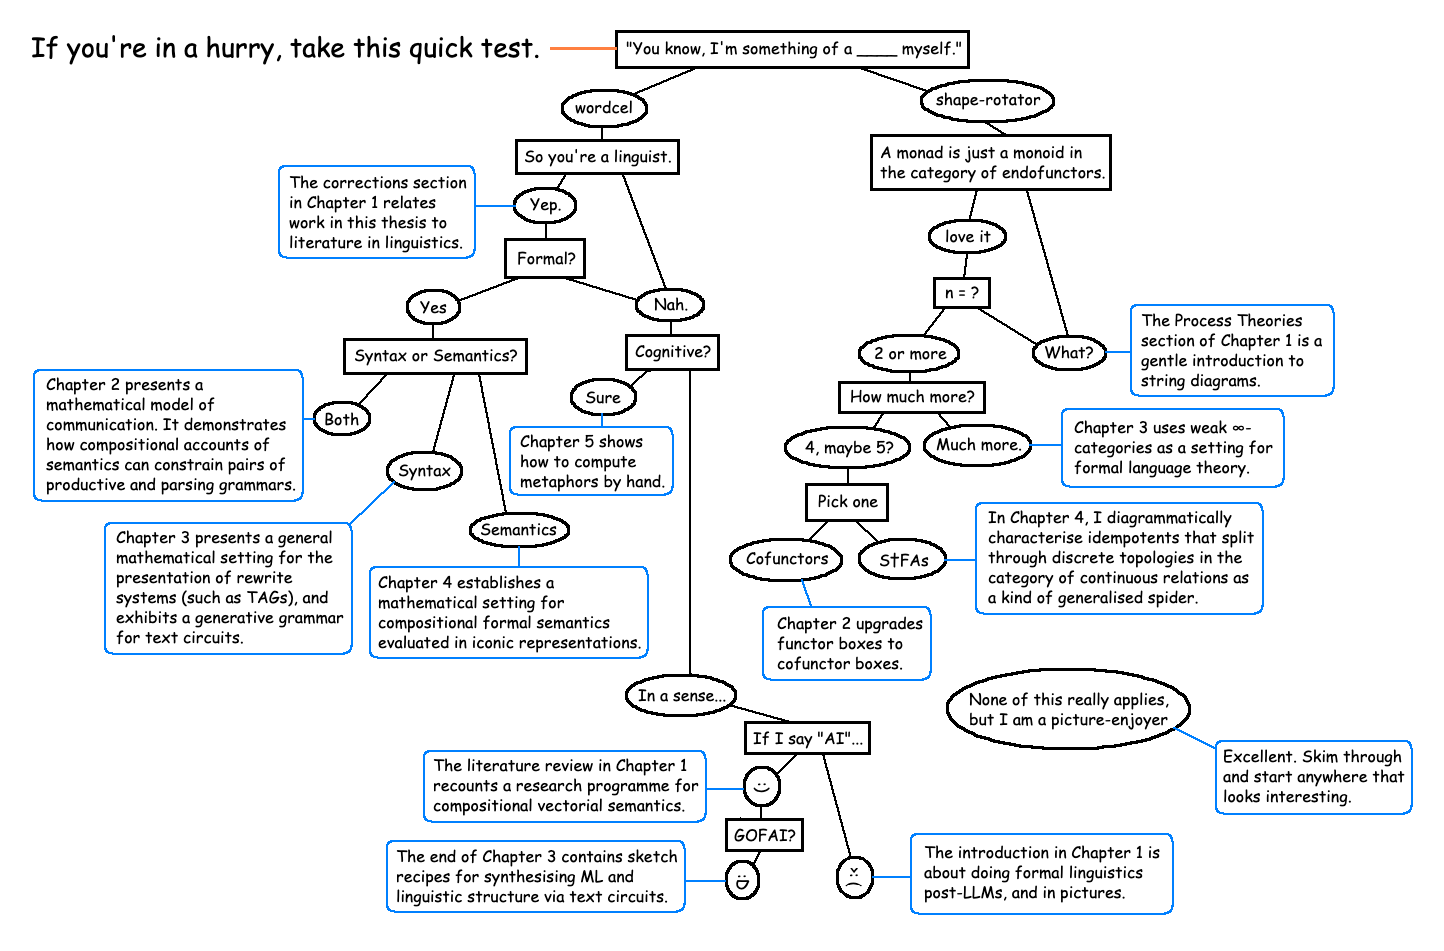
\includegraphics[width=1.5\linewidth]{figures/thesismap1.png}
\end{figure}
\clearpage

%\begin{fullwidth}
%\begin{multicols}{2}
\tableofcontents
%\end{multicols}
%\end{fullwidth}


\clearpage
\newpage
\vfill
\begin{myboxB}
\textbf{Acknowledgements}
To my parents and siblings: thank you for supporting me. I don't know how I can ever make it all up to you, but I'll try my best. I love you.\\

To my academic parents, Bob and Philipp. Thank you for your tutelage. I am glad to have found brothers in life such as you, and I hope we can tell many more stories together.\\

To my seniors --- Dan and Konstantinos here at Oxford; Jamie in Cambridge, Dusko through our letters; Salvadore, Beau and Sean throughout our time at LPPRD; Luciano and Rosaria at those wonderful meetings at the OII; Martha and Mehrnoosh and Moortgat at ESSLI; David and David and Brendan at Topos in sunny California; Pawel and Amar in (less sunny) Estonia; and Tim from across the desk-castle. You walked far along the paths I am still only just setting out on. Thank you for sharing your lessons with me.\\

A special thanks for you, Jules and Stefano. You actually read the whole damn thing and sat with me through six and a half hours of viva. It was an honour to get doctored by you.\\

To my cohort, both in Oxford --- Nick, Nicola Lukas, Guillaume, Cole, Sivert, Nihil, James, Matt --- and elsewhere --- Mario, Elena, Chad, Nathan, Bruno, Matteo, Eigil --- COVID made for an unusual DPhil, but I wouldn't have had it any other way because of you. Thank you for teaching me so much.\\

To Jono, Ben, Razin, Lia, Hamza, and Tiffany. I'm sorry for whatever part I played in getting you into this language business, it seemed like a good idea at the time. I hope at least it's a springboard towards better things. For Jono in particular: thanks for qualming.\\

To Aleks, Ilyas, and the little demon who helps me convert various drugs into diagrams and text at the cost of my health: thank you for the environments you have looked after, within which this thesis was made logistically possible.\\

To my future council of godfathers for my son Felix: Andrew, Colin, Maxim, Will, and Joel. Thank you for putting up with me and keeping me grounded.\\

Paulina, my love. Thank you for sticking with me and helping me grow. Nothing is as important to me as being happy together with you.
\end{myboxB}
\clearpage
\begin{myboxB}
\textbf{Novel contributions:}
\begin{itemize}

\item Section \ref{sec:weakn} is a pedestrian introduction to weak $n$-category theory (via \texttt{homotopy.io}, underpinned by the theory of associative $n$-categories) from the perspective of generalising familiar string-rewrite systems to higher dimensions. The chief development of this section is a demonstration that context-free grammars and tree-adjoining grammars may be formalised in the $n$-categorical setting.

\item Section \ref{sec:gencirc} spells out a generative grammar for text using an $n$-categorical signature as a rewrite system, which additionally provides a unified framework from which the Text Circuit Theorem first proved in \citep{wang-mascianica_distilling_2023} is recovered.

\item Section \ref{sec:contrelintro} introduces the category \textbf{ContRel} of continuous relations. I detail the relationships (or lack thereof) of \textbf{ContRel} to its cousins \textbf{Top} and \textbf{Rel} in Section \ref{sec:contrelmath}. Though \textbf{ContRel} is constructed na\"{i}vely, its definition and an exposition of its expressivity from the monoidal perspective appears to be novel.

\item Section \ref{sec:stickyspider} string-diagrammatically characterises set-indexed collections of disjoint open subsets of spaces in \textbf{ContRel} as \emph{sticky spiders} -- special frobenius algebras that satisfy certain interaction relations with an idempotent. The diagrammatic outcome is that reasoning with such set-indexed collections remains as graphically intuitive as with spiders.

\item Section \ref{sec:concepts} string-diagrammatically characterises a vocabulary of linguistic topological relations in \textbf{ContRel} such as simple connectedness, touching, insideness, and rigid motion.

\item Section \ref{sec:miracle} argues for the centrality of explaining communication as a criterion for formal approaches to syntax, and explores the relationship between productive and parsing grammars as organised by a monoidal cofunctor. A diagrammatic treatment of monoidal cofunctor boxes is introduced for this purpose.

\item Section \ref{sec:monty} is a standalone introduction to the mathematical setup of Montague's \emph{Universal Grammar}, aimed at modern algebraists. An outcome of this section is the placement of text circuits as a natural mathematical development in the broadly conceived programme of Montague Semantics.

\item Subsection \ref{subsec:toptext} constructs a subcategory of sticky spiders in \textbf{ContRel} on the unit square that behaves as a model of \textbf{FinRel} equipped with a Turing object, and argues for its relevance in formal semantics.

\item In Section \ref{sec:metaphor}, by parsing text as circuits (Section \ref{sec:gencirc}) and using merge-boxes (Section \ref{sec:miracle}) to interpret those circuits in \textbf{ContRel} as iconic representations equipped with a vocabulary of lingustic-topological concepts (Section \ref{sec:concepts}), I show how one may compute metaphors by hand.

\end{itemize}
\end{myboxB}
\vfill
\clearpage
\newpage

\chapter{Context and synopsis}
There are potentially practical and theoretical benefits to a fresh mathematical take on basic linguistics. String diagrams are formal, intuitive, expressive, fun, and pretty. I review the relevant research context.
\clearpage
\newpage
\section{What this thesis is about}

\begin{marginfigure}
\centering
\[\resizebox{0.5\textwidth}{!}{\tikzfig{intro/model}}\]
\caption{Let's say that \textbf\emph{{the meaning of text is how it updates a model.}} So we start with some model of the way things are, modelled as data on a wire.}
\end{marginfigure}

\begin{marginfigure}
\centering
\[\resizebox{0.6\textwidth}{!}{\tikzfig{intro/model2}}\]
\caption{Text updates that model; like a gate updates the data on a wire.}
\end{marginfigure}

\begin{marginfigure}
\centering
\[\resizebox{0.7\textwidth}{!}{\tikzfig{intro/model3}}\]
\caption{Text is made of sentences; like a circuit is made of gates and wires.}
\end{marginfigure}

\begin{marginfigure}
\centering
\[\resizebox{0.8\textwidth}{!}{\tikzfig{intro/model4}}\]
\caption{Let's say that \textbf{\emph{The meaning of a sentence is how it updates the meanings of its parts.}} As a first approximation, let's say that the \emph{parts} of a sentence are the nouns it contains or refers to. Noun data is carried by wires. Collections of nouns are related by gates, which play the roles of verbs and adjectives.}
\end{marginfigure}

\begin{marginfigure}
\centering
\[\resizebox{0.9\textwidth}{!}{\tikzfig{intro/model5}}\]
\caption{Gates can be related by higher order gates, which play the roles of adverbs, adpositions, and conjunctions; anything that modifies the data of first order gates like verbs.}
\end{marginfigure}

\begin{marginfigure}
\centering
\[\resizebox{\textwidth}{!}{\tikzfig{intro/model6}}\]
\caption{In practice, higher order gates may be implemented as gates that modify parameters of other gates. Grammar, and \emph{function words} -- words that operate on meanings -- are in principle absorbed by the geometry of the diagram. These diagrams are natural vehicles for \emph{dynamic semantics}, broadly construed, where states are prior contexts and sentences-as-processes update prior contexts.}
\end{marginfigure}

\marginnote{
\begin{defn}[Text Circuits]
\emph{Text circuits} are made up of three ingredients:
\begin{itemize}
\item wires
\item boxes, or gates
\item boxes with holes that fit a box, or 2nd order gates
\end{itemize}
\end{defn}
}

\begin{marginfigure}
\centering
\[
\tikzfig{textcirc/nounwiresABN} 
\]
\caption{Nouns are represented by wires, each `distinct' noun having its own wire.}
\end{marginfigure}

\begin{marginfigure}
\centering
\[
\tikzfig{textcirc/ADJgate} \quad\quad\quad \tikzfig{textcirc/IVgate} \quad\quad\quad \tikzfig{textcirc/TVgate}
\]
\caption{We represent adjectives, intransitive verbs, and transitive verbs by gates acting on noun-wires. Since a transitive verb has both a subject and an object noun, that will then be two noun-wires, while adjectives and intransitive verbs only have one.}
\end{marginfigure}

\begin{marginfigure}
\centering
\[
\tikzfig{textcirc/ADVbox}
\]
\caption{Adverbs, which modify verbs, we represent as boxes with holes in them, with a number of dangling wires in the hole indicating the shape of gate expected, and these should match the input- and output-wires  of the box with the whole.}
\end{marginfigure}

\begin{marginfigure}
\centering
\[
\tikzfig{textcirc/ADPIVbox}
\]  
\caption{Similarly, adpositions also modify verbs, by moreover adding another noun-wire to the right.}
\end{marginfigure}

\begin{marginfigure}
\centering
\[
\tikzfig{textcirc/SCVbox}
\]
\caption{For verbs that take sentential complements and conjunctions, we have families of boxes to accommodate input circuits of all sizes. They add another noun-wire to the left of a circuit.}
\end{marginfigure}

\begin{marginfigure}
\centering
\[
\tikzfig{textcirc/CNJbox2}
\]
\caption{Conjunctions are boxes that take two circuits which might share labels on some wires.}
\end{marginfigure}

\begin{marginfigure}
\centering
\[
\tikzfig{textcirc/ADPIVgate}
\]
\caption{Of course filled up boxes are just gates.}
\end{marginfigure}

\begin{marginfigure}
\centering
\[
\tikzfig{textcirc/gatecompex1}  
\]
\caption{Gates compose sequentially by matching labels on some of their noun-wires and in parallel when they share no noun-wires, to give \underline{text circuits}.}
\end{marginfigure}

\begin{marginfigure}
\centering
\resizebox{\marginparwidth}{!}{\tikzfig{textcirc/circgen1}}
\caption{To summarise: composition by nesting corresponds to grammatical structure within sentences. Sentences correspond to filled gates, boxes with fixed arity correspond to first-order modifiers such as adverbs and adpositions, and boxes with variable arity correspond to sentential-level modifiers such as conjunctions and verbs with sentential complements.}
\end{marginfigure}

\begin{marginfigure}
\centering
\resizebox{0.75\marginparwidth}{!}{\tikzfig{textcirc/circgen2}}
\caption{Composition by connecting wires corresponds to identifying coreferences in discourse. We obtain the same circuit for multiple text presentations of the same content, e.g. \texttt{Sober Alice who sees drunk Bob clumsily dance laughs at him.} yields the same circuit as the text \texttt{Alice is sober. She sees Bob clumsily dance. Bob is drunk. She laughs at him.}}
\end{marginfigure}

\newthought{This thesis is about studying language using string diagrams.}

I am interested in using contemporary mathematical tools as a fresh approach to modelling some features of natural language considered as a formal object. Specifically, I am concerned with the compositional aspect of language, which I seek to model with the compositionality of string diagrams. Insofar as compositionality is the centrepiece of `knowledge of language', I share a common interest with linguists, but I will not hold myself hostage to their methods, literature, nor their concern with empirical capture. I will make all the usual simplifying assumptions that are available to theoreticians, such that an oracular machine will decide on lexical disambiguation and the appropriate parse using whatever resources it wants, so that I am left to work with lexically disambiguated words decorating some formal grammatical structure. It is with this remaining disambiguated mathematical structure that I seek to state a general framework for \emph{meaningful compositional representations of text}, in the same way we humans construct rich and interactable representations of things-going-on in our minds when we read a storybook. So if you are interested in understanding language, this thesis is an invitation to a conception of formal linguistics that's maybe worth a damn in a world where large language models exist.

\newthought{\textbf{Objection}: Isn't that reinventing the wheel?}

Yes, to an extent. I am not interested in the human language faculty \emph{per se}, so my aims differ. There are several potential practical and theoretical benefits that a fresh mathematical perspective on language enables. First, the mathematics of applied category theory allows us to unify different views of syntax, and conservatively generalise formal semantics to aspects of language that may have seemed beyond the reach of rigour, such as metaphor. Practically, the same mathematics allows us to construct interfaces between syntax/structure and semantics/implementation in such a way that we can control the former and delegate the latter by providing specifications without explicit implementation, which (for historical reasons I will explain shortly) is possibly the least-bad idea for getting at natural language understanding in computers from the bottom-up. Second, there are probably benefits to expressing linguistics in the same mathematical and diagrammatic lingua franca that can be used to represent and reason -- often soundly and completely -- about linear and affine algebra \citep{sobocinski_graphical_2015,bonchi_interacting_2017,bonchi_graphical_2019}, first order logic \citep{haydon_compositional_2020}, causal networks \citep{lorenz_causal_2023,jacobs_causal_2019}, signal flow graphs \citep{bonchi_categorical_2014}, electrical circuits \citep{boisseau_string_2022}, game theory \citep{hedges_string_2015}, petri nets \citep{baez_open_2020}, probability theory \citep{fritz_finettis_2021}, machine learning \citep{cruttwell_categorical_2022}, and quantum theory \citep{coecke_interacting_2011,coecke_picturing_2017,poor_completeness_2023}, to name a few applications. At the moment, the practical achievements of language algorithms de-emphasise the structure of language, and there is no chance of reintroducing the study of structure with dated mathematics.

\newthought{\textbf{Point of information:} What do you mean by natural language?}

Natural language is a human superpower, and the foundation of our collective achievements and mistakes as a species. By \emph{natural language} I mean a non-artificial human language that some child has grown up speaking. English is a natural language, while Esperanto and Python are constructed languages. If you are still reading then you probably know a thing or two already about natural language. Insofar as there are rules for natural languages, it is probable that like most natural language users, you obey the rules of language intuitively without knowing what they are formally; for example while you may not know what adpositions are, you know where to place words like \texttt{to}, \texttt{for}, \texttt{of} in a sentence and how to understand those sentences. At a more complex level, you understand idioms, how to read between the lines, how to flatter, insult, teach, promise, wager, and so on. There is a dismissive half-joke that "engineering is just applied physics", which we might analogise to absurdity as "law is just applied linguistics"; in its broadest possible conception, linguistics is the foundational study of everything that can possibly be expressed.

\newthought{\textbf{Point of information:} What are string diagrams?}

String diagrams are a pictorial syntax for interacting processes. They are compositional blueprints that we can give semantics to -- i.e. instantiate -- in just about any system with a notion of sequential and parallel composition of processes. In particular, this means string diagrams may be interpreted as program specifications on classical or quantum computers, or as neural net architectures. Moreover, we can devise equations between string diagrams to govern the behaviour of each process without having to spell out a bottom-up implementation, by asking processes to interact with other processes in certain ways. The mathematical foundation of string diagrams -- applied category theory -- is in short, the mathematics of compositionality.\\

Many fields of study have developed string diagrams as informal calculational aids, unaware of their common usage across disciplines and the rather new mathematics that justifies their use; everybody knows, but it isn't common knowledge. Why is that so? Because just as crustaceans independently converge to crab-like shapes within their own ecological niches by what is called \emph{carcinisation}, formal notation for formal theories of "real world" problem domains undergo "string-diagrammatisation" in similar isolation. Why is that so? Because our best formal theories of the real world treat complexity as the outcome of composing simple interacting parts; perhaps nature really works that way, or we cannot help but conceptualise in compositional terms. When one has many different processes sending information to each other via channels, it becomes tricky to keep track of all the connections using one-dimensional syntax; if there are $N$ processes, there may be on the order of $\mathcal{O}(N^2)$ connections, which quickly becomes unmanageable to write down in a line, prompting the development of indices in notation to match inputs and outputs. In time, probably by doodling a helpful line during calculation to match indices, link-ed indices become link-ing wires, and string-diagrammatisation is complete.\\

I will demonstrate how they are used in Section \ref{sec:proctheory} and define them formally in Section \ref{sec:diagdefs}. String diagrams are a heuristically natural yet mathematically formal syntax for representing complex, composite systems. I say \emph{mathematically formal} to emphasise that string diagrams are not merely heuristic tools backed by a handbook of standards decided by committee: they are unambiguous mathematical objects that you can bet your life on \citep{joyal_geometry_1991,joyal_geometry_nodate,maclane_natural_1963,lane_categories_2010,selinger_survey_2010}.

\section{\textbf{Question:} What is the practical value of studying language when Large Language Models exist?}
Large language models raise questions of existential concern for the field of linguistics. More narrowly, they demand justification as to why I am writing a thesis about theoretical approaches to basic linguistics as a computer scientist in current year. Although this thesis is pure theory, I wish to address the question of practical value early because I imagine practical people are impatient.

\newthought{Let me outline the terms and stakes.} Because the field is developing so quickly, assume that everything about LLMs is prefaced with "at the time of writing". Large Language Models are programs trained -- using a lot of data and a lot of compute time -- to predict the next word in text, computational techniques for which have evolved from Markov n-grams to transformers \citep{vaswani_attention_2017}. This sounds unimpressive, but -- in tandem with fine-tuning from human feedback in the case of chatGPT \citep{openai_chatgpt_2022} -- it is enough to tell and explain jokes \citep{bastian_google_2022}, pass the SAT \citep{teddy_teddynpc_i_2022} and score within human ranges on IQ tests \citep{thompson_gpt-35_2022}. There is an aspect of genuine scientific and historical surprise that text-prediction can do this kind of magic. On the account of \citep{mcshane_linguistics_2021}, computational linguistics began in a time when compute was too scarce to properly attempt rationalist, knowledge-based and theoretically-principled approaches to modelling language. Text-prediction as a task arose from a deliberate pursuit of "low-hanging fruit" as a productive and knowledge-lean alternative to doing nothing in an increasingly data-rich environment. Some observers \citep{church_pendulum_2011} expressed concern that all this fruit would be picked bare in a generation to force a return to knowledge-based methods, but those concerns appear now to be unfounded.\\

I'm sure there will be many further notable developments, and to be safe I won't make any claims about what machines can't do if we keep making them bigger and feed them more data or have them interact with one another in clever ways. Nonetheless there remain limitations that seem persistent for the foreseeable future, not in terms of \emph{capabilities}, but in terms of \emph{explainability and safety}. These models have a tendency to hallucinate facts and (ironically, for a computer) bad arithmetic \citep{hendrycks_measuring_2021}, and I imagine that the cycle of discovering limitations and overcoming them will continue. Despite whatever limitations exist in the state-of-the-art, it is evident to all sane observers that this is an important technology, for several reasons.

\begin{enumerate}
\item{
LLMs are a civilisational milestone technology. A force-multiplication tool for natural language -- the universal interface -- built from abundant data and compute in the information age may have comparably broad, deep, and lasting impact to the conversion of abundant chemical fuel to physical energy by steam engines in the industrial revolution.
}
\item{
LLMs represent a paradigm shift for humanity because they threaten our collective self-esteem, in a more pointed manner than losing at chess or Go to a computer; modifying a line of thinking from \citep{floridi_fourth_2014}, LLMs demonstrate that language and (the appearance of) complex thought that language facilitates is not a species-property for humans, and this stings on par with Darwin telling us we are ordinary animals like the rest, or Galileo telling us our place in the universe is unremarkable.
}
\item{
LLMs embody the latest and greatest case study of the bitter lesson \citep{sutton_bitter_2019}. The tragedy goes like this: there's a group of people who investigate language -- from syntax and semantics to pragmatics and analogies and storytelling and slang -- who treat their subject with formal rigour and have been at it for many centuries. Their role in the story of LLMs is remarkable because it doesn't exist. They were the only qualified contestants in a "let's build a general-purpose language machine" competition, and they were a no-show. Now the farce: despite the fact that all of their accumulated understanding and theories of language were left out of the process, the machine is not only built but also far exceeds anything we know how to build in a principled way out of all their hard-earned insight. That is the bitter lesson: dumb methods that use a lot of data and compute outperform clever design and principled understanding.
}
\end{enumerate}

I will note in passing that I have an ugly duckling problem, in that I am not strictly aligned with machine learning, nor linguists broadly construed, nor mathematical linguists. I am unfortunately placed in that I feel enough affinity to have defensive instincts for each camp, but I am distanced enough from each that I am sure to suffer attacks from all sides. Perhaps a more constructive metaphor than war is that I am writing in a cooperative spirit between domains, or that I am an arbitrageur of ideas between them. With that in mind, I am for the moment advocating on behalf of pen-and-paper-and-principles linguists in formulating a two-part reply to the devastating question, and I will switch sides later for balance. First a response that answers with practical values in mind, and then a response that asserts and rests upon the distinct values of linguists.

\section{\textbf{First Reply:} I don't know. Maybe explainability, maybe something else.}

\newthought{Expressing grammar as composition of processes might yield practical benefits. Moreover, we want economy, generality, and safety for language models, and we can potentially do that with few tradeoffs if we use the right framework.}

Simplified, half of the problem of learning language is learning the meaning of words. The meanings change over time and are context-dependent, and the words are always increasing in number. Encoding these meanings by hand is a sisyphean task. Data-driven learning methods are a good fit: the patterns to be learnt are complex and nebulous, and there is a lot of data. However, data-driven methods may be weaker at the second half of the problem: learning and executing the composition of meanings according to syntax. We can see just how much weaker when we consider the figures involved in 'the poverty of the stimulus'.\\

In short, this famous problem is the observation that humans learn language despite having very little training data, in comparison to the complexity of the learned structure. It is on the basis of this observation -- alongside many others surrounding language acquisition and use -- that Chomsky posits \citep{chomsky_new_2000} that language is an innate human faculty, the development of which is less like effortfully going to the gym and more like effortlessly growing arms you were meant to have. The explanation goes like this: we can explain how a complex structure like grammar gets learnt from a small amount of data if everyone shares an innate Universal Grammar with a small number of free parameters to be learned. Whether or not the intermediate mechanism is a species-property of humans, the point is that we humans get a very small amount of input data, that data interacts with the mechanism in some way, and then we know a language. So, now that there are language-entities that are human-comparable in competence, we can make a back-of-the-envelope approximation of how much work the intermediate mechanism is doing or saving by comparing the difference in how much data and compute is required for both the human and for the machine to achieve language-competence. Humans get about 1.5 megabytes of data \citep{mollica_humans_2019}, 90 billion neurons \citep{herculano-houzel_remarkable_2012}, and an adult human consumes around 500 calories per day for thinking, for let's say 20 years of language learning. Rounding all values \emph{up} to the closest order of magnitude, this comes to a cost metric of $10^{29} \ \text{bits} \times \text{joules} \times \text{neurons}$. PaLM -- an old model which is by its creators' account the first language model to be able to reason and joke purely on the basis of linguistic ability and without special training \citep{chowdhery_palm_2022,narang_pathways_2022} -- required 780 billion training tokens of natural language (let's discount the 198 gigabytes of source code training data), which we generously evaluate at a rate of 4 characters per token \citep{khan_what_2023} and 5 bits per character. The architecture has 540 billion neurons, and required 3.2 million kilowatt hours of energy for training \citep{tom_goldstein_tomgoldsteincs_training_2022}. Rounding values for the three units down \emph{down} to the nearest order of magnitude comes to a cost metric of $10^{41}$ bit-joule-neurons. Whatever the human mechanism is, it is responsible for an order of magnitude in efficiency \emph{give or take an order of magnitude of orders of magnitude}. It's possible that over time we can explain this difference away by various factors such as the efficiency of meat over minerals, separating knowledge of the world from knowledge of language, more efficient model architectures, or the development of efficient techniques to train new language models using old ones \citep{taori_rohan_stanford_2023}. One thing is clear: if it is worth hunting a fraction of a percent of improvement on a benchmark, forget your hares, a $10^{10}$ factor is a stag worth cooperating to feast on.\\

\newthought{The linguistic strategy for hunting the stag starts with what we know about how the mechanism between our ears works with language.} The good news is that the chief methodology of armchair introspection is egalitarian and democratic. The bad news is that it is also anarchistic and hard-by-proximity; we are like fish in water, and it is hard for fish to characterise the nature of water. So the happy observations are difficult to produce and easily verified, and that means there are just a few that we know of that are are unobjectionably worth taking into account. One, or \emph{the} such observation is \emph{systematicity}. Systematicity \bR CITE \e refers to when a system can (generate/process) infinitely many (inputs/outputs/expressions) using finite (means/rules/pieces) in a "consistent" (or "systematic") manner -- some tautologies require geniuses like Fodor to put into words. Like pornography, examples are easier than definitions. We know finitely many words but we can produce and understand infinitely many texts; we can make infinitely many lego sculptures out of finitely many types of pieces; we can describe infinite groups and other mathematical structures using finitely many generators and relations; in the practical domain of computers, systematicity is synonymous with programmability and expressibility.\\

The concepts of systematicity and compositionality are deeply linked, because the only way we know how to achieve systematicity in practice is composition. Frege's initial conception of compositionality \citep{frege_gottlob_selbst_1884} was borne of meditations on language, and states that a whole is the sum of its parts -- some tautologies require geniuses like Frege to put into words. Later conceptions of compositionality, the most notable deviation arising from meditations on quantum theory, are the same as the original, modulo variations on the formal definitions of parts and the method of summation \citep{coecke_compositionality_2021}. So there is our starting point: language is systematic and systematicity is the empirical surface of compositionality as far as we know, so compositionality is probably part of the solution to the problem of the stimulus, if not most of it.\\

The reasoning I report above should clarify why some folks don't think large language models have anything to do with language. The issue with purely data-driven architectures is either that we know immediately that they cannot be operating upon their inputs in a compositional way, or even if they do appear to be doing compositional things, their innards are too large and their workings too opaque to tell with confidence. Insofar as the task of learning language splits between learning meanings and learning the compositional rules of syntax that give rise to systematicity, I hope the framework I present in this thesis can be a proposal to split the cake sensibly between the two halves of the problem: meanings for the machines, compositionality for the commons. Syntax is still difficult and vast, but the rules are finite and relatively static. We can break the black-box by reexpressing syntax as the composition of smaller black-boxes. We all stand to benefit: we may give machines an easier time -- now they only have to learn the meanings of words well -- and we can have confidence that the internal representations of the machine -- their "mind's eye" -- contains something we can probe and understand.

\subsection{\textbf{Objection:} You're forgetting the bitter lesson.}

The bitter lesson is so harsh and often-enough repeated that this viewpoint is worth addressing proactively. The caveat that saves us is that the curse of expertise applies only to the object-language of the problem to be solved, not model architectures. We agree that qualitative improvements in problem-solving ability rarely if ever arise from encoding expert knowledge of the problem domain. Instead -- and we see this historically, tracking the evolutionary path for data-driven language models from markov chains to deep learning \citep{lecun_deep_2015}, RNNs \citep{rumelhart_learning_1987}, LSTMs \citep{hochreiter_long_1997}, and now transformers \citep{vaswani_attention_2017} -- these improvements come from \emph{architectural} innovations, which means altering the parts and internal interactions of a model: changing \emph{how} it thinks rather than \emph{what} it thinks, to paraphrase Sutton's original prescription. These structural changes are motivated by understandings (at varying degrees of formality) of the "geometry of the problem" \citep{bronstein_geometric_2021}. The value proposition here is that with an appropriate mathematical lingua franca for structure, composition, and interaction, we can mindfully design rather than stumble upon the "meta-methods" Sutton calls for, allowing experts to encode \emph{how} machines think and discover rather than \emph{what}. I hope to demonstrate in \bR Section \ref{} \e how importing compositional and structural understanding from linguistics to machine learning via string diagrams might allow us to cheat the bitter lesson in spirit while adhering to the letter.

\subsection{\textbf{Objection:} GOFAI? GO-F-yourself.}
 
Hostility (or at least indifference) to symbolic approaches is a stance espoused by virtually all of modern machine learning, and for good reasons. This stance is worth elaborating and steelmanning for pen-and-paper-people in the context of language. First, many linguistic phenomena are nebulous \citep{chapman_david_nebulosity_2010}: the boundary of a simile is like that of a cloud, not sharp like the boundary of a billiard ball. Second, linguistic phenomena are complex, dynamic, and multifactorial: there are so many interacting mechanisms and forces in the production and comprehension of language that even if we do have crisp mathematical models for all the constituent processes we are still left with something computationally irreducible. These two points together weakly characterise the kinds of problem domains where machine learning shines. It is just fact that LLM outputs today conform to any reasonable understanding of syntax, semantics, pragmatics, conversational implicature, and whatever else we have theorised. It is just a fact that they produce better poetry and humor than anything we could explicitly program according to our current understanding. It is almost a natural law that they will only get better from here.\\

So what good are pen-and-paper theories as far as practical applications are concerned? To borrow terms from concurrency, there is already plenty of liveness, what is needed is more safety; liveness is when the program does something good, and safety is a guarantee it won't do something bad. For example, there is ongoing work in integrating LLMs with stuctured databases for uses where facts and figures and ontologies matter; there is still a need for safeguards to prevent harmful outputs and adversarial attacks like prompt injection; while LLMs give a very convincing impression of reasoned thought, we would like to be sure if ever we decide to use such a machine for anything more than entertainment, such as assisting a caregiver in the course of healthcare decisions.\\

The good news is that symbolic-compositional theories are the right shape for safety concerns, because they can be picked apart and reasoned about. It is clear however that symbolic-compositional approaches by themselves are nowhere near achieving the kind of liveness LLMs have. Therefore, the direction of progress is synthesis.

\subsection{\textbf{Point of Information:} What is computational irreducibility?}

\emph{Computational irreducibility} \citep{wolfram_new_2002}, elsewhere called "type 2" problems \citep{marr_artificial_1977}, refers to a special kind of computational difficulty where the explanation of a system amounts to a total computational simulation of it. This is best understood by example. We have a closed-form mathematical expression to shortcut the computation of the evolution of a system of two point masses under gravity, but we have no such shortcut for the three-body problem; the best we can do is simulate the system's evolution, and an inconvenient fact is that even for very simple systems, it is possible that no amount of causal-mechanistic understanding will simplify compututational simulation.

\subsection{\textbf{Objection:} How does any of this improve capabilities?}

It's not meant to. The core value proposition for synthesis is explainable AI, which operates in a manner we can analyse, and if appropriate, constrain. For this purpose, merely knowing \emph{what} a deep-learning model is thinking is not enough\marginnote{I recount the following from \citep{sogaard_grounding_2023}, which argues that symbol-grounding is solvable from data alone, and in the process surveys the front of the symbol-grounding problem in AI: the issue of whether LLMs encode what words refer to and mean. On the account of \citep{bender_climbing_2020}, the performance of current LLMs is a form of Chinese Room \citep{searle_minds_1980} phenomenon, so no amount of linguistic competence can be evidence that LLMs solve the symbol-grounding problem. However, the available evidence appears to suggest otherwise. For example, large models converge on word embeddings for geographical place names that are isomorphic to their physical locations \citep{lietard_language_2021}. Since we know that brain activity patterns encode abstract conceptual space with the same mechanisms as they do physical spaces \citep{kriegeskorte_grid_2016}, extrapolating the ability of LLMs to encode spatially-analogical representations would in the limit suggest that LLMs encode meanings in a way isomorphic to how we do, at least for individual tokens, and so long as we take seriously some version of G\"{a}rdenfors' \citep{gardenfors_geometry_2014} thesis that meaning is encoded geometrically.}: solving symbol-grounding alone is a necessary but insufficient component. For instance, merely knowing what the weights of subnetworks of an image classification model represent does not meet our requirement of an understanding of the computations that manipulate those representations. Moreover, purely data-driven methods to control the computation may incur ethical costs \bR CITE \e, to say nothing of the potential harm that may result from a poorly safeguarded model \bR CITE \e. Add to this the ever-growing dirty laundry lists of AI models failing \bR CITE \e in inhuman ways, and the task of incorporating compositionality -- a formal understanding of \emph{how} models learn and reason -- gains urgency.\\

The investigation of the common ground between symbolic-composition and connectionism takes on, I suggest, essentially two, dual forms. The first kind uses connectionist methods to simulate symbolic-composition, which we can see the beginnings of in LLMs by examples such as chain-of-thought reasoning \citep{wei_chain--thought_2023-1} and by probing their behaviour with respect to understood symbolic models \citep{koralus_humans_2023}. The second kind is the inverse, where connectionist architectures are organised and reasoned with by symbolic-compositional means. Some examples of the first kind include implementing data structures as operations on high-dimensional vectors, taking advantage of the idiosyncrasies of linear algebra in very high dimension \citep{kanerva_computing_2019}, or work that explores how the structure of word-embeddings in latent space encode semantic relationships between tokens. Some examples of the second kind include reasoning about the capability of graph neural networks by identifying or isolating their underlying compositional structure \citep{liu_seeing_2023}, or architectures whose behaviour arises from compositional structure using neural nets as constituent parts, such as GANs \citep{goodfellow_generative_2014} and gradient boosted decision trees \citep{chen_xgboost_2016}. The work in this thesis builds upon a research programme -- DisCoCat \citep{coecke_mathematical_2010}, elaborated in \bR Section \ref{} \e -- which lies somewhere in the middle of a duality of approaches to merging connectionism and symbolic-composition. It is, to the best of my knowledge, the only approach that explicitly incorporates mathematically rigourous compositional structures from the top-down alongside data-driven learning methods from the bottom-up. Fortifying this bridge across the aisle requires a little give from both sides; I ask only that reader entertain some pretty string diagrams.

\subsection{\textbf{Objection:} Aren't string diagrams just graphs?}

\marginnote{A deeper objection here is that diagrams do not look like serious mathematics. Later I will give ample space to show how they are serious, but the reasons behind this rather common prejudice are worth elaborating. This is the wound Bourbaki has inflicted. Nicolas Bourbaki is a pseudonym for a group of French mathematicians, who wrote a highly influential series of textbooks. It is difficult to overstate their influence. The group was founded in the aftermath of the First World War, around the task of writing a comprehensive and rigourous foundations of mathematics from the ground up. The immediate \emph{raison-d'\^{e}tre} for this project was that extant texts at the time were outdated, the oral tradition and living history of mathematics in institutions of learning in France decimated by the deaths of mathematicians at war. In a broader historical context, Bourbaki was a reactionary response to the crisis in the foundations of mathematics at the beginning of the century, elicited by Russell's paradox. Accordingly, their aims were rationalist, totalitarian, and high-modernist, favouring abstraction and disdaining visualisation, in line with their contemporary artistic and musical fashions. Consequently, Bourbaki's Definition-Proposition-Theorem style of mathematical exposition is a historical aberration: a bastardisation of Euclid that eschews intuition via illustration and specificity in favour of abstraction and generality, pretending at timelessness, requiring years of initiation to effectively read and write, and remaining \emph{de rigeur} for rigour today in dry mathematics textbooks. The deeper objection arises from the supposition that serious mathematics ought to be arcane and difficult, as most mathematics exposition after Bourbaki is. The reply is that it need not be so, and that it was not always so! The Bourbaki format places emphasis and prestige upon the deductive activity that goes into proving a theorem, displacing other aspects of mathematical activity such as constructions, algorithms, and taxonomisation. These latter aspects are better suited for the nebulous subject matter of natural language, which not lend itself well to theorems, but is a happy muse for mathematical play.}

Yes and no! This point is best communicated by a mathematical koan. Consider the following game between two players, you and me. There are 9 cards labelled 1 through 9 face up on the table. We take turns taking one of the cards. The winner is whoever first has three cards in hand that sum to 15, and the game is a draw if we have taken all the cards on the table and neither of us have three cards in hand that sum to 15. I will let you go first. Can you guarantee that you won't lose? Can you spell out a winning strategy? If you have never heard this story, give it an honest minute's thought before reading on.\\

The usual response is that you don't know a winning strategy. I claim that you probably do. I claim that even a child knows how to play adeptly. I'll even wager that you have played this game before. The game is Tic-Tac-Toe, also known as Naughts-and-Crosses: it is possible to arrange the numbers 1 to 9 in a 3-by-3 magic square, such that every column, row, and diagonal sums to 15.\\

The lesson here is that choice of representations matter. In the mathematical context, representations matter because they generalise differently. On the surface, here is an example of two representations of the same platonic mathematical object. However, Tic-Tac-Toe is in the same family as Connect-4 or 5-in-a-row on an unbounded grid, while the game with numbered cards generalises to different variants of Nim. That they coincide in one instance is a fork in the path. In the same way, viewing string diagrams as "just graphs" is taking the wrong path, just as it would be true but unhelpful to consider graphs "just sets of vertices and edges". String diagrams are indeed "just" a special family of graphs, just as much as prime numbers are special integers and analytic functions are special functions. Throughout this thesis I will be re-presenting familiar and unfamiliar things in string diagrams, so I request the reader to remember the koan and keep an open mind.\\

In a broader context, representations matter for the sake of improved human-machine relations. These two representations are the same as far as a computer or a formal symbol-pusher is concerned, but they make world of difference to a human native of meatspace. We ought to swing the pendulum towards incorporating human-friendly representations in language models, so that we may audit those representations for explainability concerns. As it stands, there is something fundamentally inhuman and behavioural about treating the production of language as a string of words drawn from a probability distribution. I don't know about you, but I tend to use language to express pre-existing thoughts in my head that aren't by nature linguistic. Even if we grant that the latent space of a data-driven architecture is an analog for the space of internal mental states of a human user of language, how can we know whether the spaces are structurally analogous to the extent that human-machine partnership through the interface of natural language is safe? So here again is the possible solution: by composing architectures in the shape of language from the start, we can attempt guarantees that the latent-space representation of the machine is built up in the same way we build up a mental representation when we read a book or watch a film. I'll sketch how to approach this in \bR Section \ref{} \e.

\section{\textbf{Second Reply:} LLMs don't help us understand language; how might string diagrams help?}

Another way to deal with the devastating question of LLMs is to reject it, on the basis that using or understanding LLMs is completely different from understanding language, and language is worth understanding in its own right. To illustrate this point by a thought experiment, what would linguistics look like if it began today? LLMs would appear to us as oracles; wise, superhumanly capable at language, but inscrutable. Similarly, most people effortlessly use language without a formal understanding which they can express. So the fundamental mystery would remain unchanged. Understanding how an LLM works cannot help: to borrow a thought from \bR CITE \e, suppose you knew the insides of a mechanical calculator by heart. Does that mean you \emph{understand} arithmetic? At best, obliquely: implementing a computer for ideal arithmetic means compromises; the calculator is full of inessentialities and tricks against the constraints of physics. You would not know where the tricks begin and the essence ends. Similarly, suppose you knew every line of code and every piece of data used to train an LLM; does that mean you understand how language works? How does one delineate what is essential to language, and what is accidental? So the value proposition to establish is how string diagrams come into the picture for the linguist who is (definitionally) concerned with understanding how language works. Let's entertain one more objection from the practical reader and one objection from the theoretical reader before formulating a reply.

\subsection{\textbf{Objection:} Isn't the better theory the one with better predictions?}

Whether LLMs are even a theory of language is a best debatable. There are various criteria -- not all independent -- that are arguably necessary for something to qualify as an explanatory theory, and while LLMs satisfice (or even excel) at some, they fail at others. Empirical adequacy -- the ability of theory to account for the available empirical data and make good predictions about future observations -- is one such criterion \bR CITE \e, and here LLMs excel. In constast to the idealised and partial nature of formal theories, the nature of LLMs is that they are trained on empirical data about language that captures the friction of the real world. So, in terms of raw predictive power, we should naturally expect the LLMs to have an advantage over principled theories. They are so good at empirical capture that to some degree they automatically satisfy the related criteria of coherence -- consistency with other established linguistic theories -- and scope -- the ability to capture a wide range of phenomena. But while empirical capture is necessary for explanatory theories, it is insufficient.\\

\marginnote{To illustrate the insufficiency of empirical capture to make a theory, consider the historical case study of models of what we now call the solar system. The Ptolemaic geocentric model of the solar system was more empirically precise than the heliocentric Copernican, even though the latter was "more correct" \bR CITE \e. This should not be surprising, because Ptolemaic epicycles can overfit to approximate any observed trajectory of planets. It took until Einstein's relativity to explain the precession of perihelion of mercury, which at last aligned theoretical understanding with empirical observation. But Newton's theory of gravity was undeniably worthwhile science, even if it was empirically outperformed by its contemporaries. Consider just how divorced from reality Newton was: Aristotelian physics is actually correct on earth, where objects don't continue moving unless force is continually supplied, because friction exists. It took a radical departure from empirical concerns to the frictionless environment of space in order obtain the simplified and idealised model of gravity that is the foundation of our understanding of the solar system and beyond. The lessons as I see them are as follows. First, aimed towards some advocates of theory-free approaches, we should belay the order to evacuate linguistics departments because performance is to some degree orthogonal to understanding. In fact, the scientific route of understanding involves simplified and idealised models that ignore friction, and will necessarily suffer in performance while maturing, so one must be patient. Second, aimed towards some theoreticians, haphazard gluing together of different theories and decorating them with bells-and-whistles for the sake of fitting empirical observation is no different than adding epicycles; one must either declare a foundational or philosophical justification apart from empirical capture (which machines are better at anyway), or state outright that it's just a fun hobby. Third, while explainability studies in terms of analysing the behaviour of subnetworks is practically important, the whole approach seems fundamentally misguided; imagine an epicyclist explaining the precession of mercury's perihelion by pointing at a collection of epicycles and calling it a "distributed representation".}

There are several criteria where the adequacy of LLMs is unclear or debatable. Fruitfulness is a sociological criterion for goodness of explanatory theories, in that they should generate new predictions and lead to further discoveries and research \bR CITE \e. While they are certainly a potent catalyst for research in many fields even beyond machine learning, it is unclear for now how they relate to the subject matter of linguistics. Whether they satisfy Popper's criterion of falsifiability is as of yet not determined, because it is not settled how to go about falsifying the linguistic predictions of LLMs, or even express what the content of a theory embodied by an LLM is. The closest examples to falsifiability that come to mind are tests of LLM fallibility for reasoning and compositional phenomena \bR CITE \e, or their weakness to adversarial prompt-injections \bR CITE \e, but these weaknesses do not shed light on their linguistic competence and "understanding" directly.\\

Now the disappointments. LLMs are far from simple, and simplicity (Occam's Razor) is an ancient criterion for the goodness of explanation. Moreover, they fail at providing explanatory mechanisms \bR CITE \e, and they do not unify or subsume our prior understandings \bR CITE \e. The first two points are unobjectionable, so I will briefly elaborate on the criterion of unification and subsumption of prior understandings, borrowing a framework from cognitive neuroscience. A common methodology for investigating cognitive systems is Marr's 3 levels \bR CITE \e (poorly named, since they are not hierarchical, but more like interacting domains.) Level 1 is the computational theory, an extensional perspective that concerns tasks and functions: at this level on asks what the contents and aims of a system are, to evaluate what the system is computing and why, respectively. Level 2 is representation and algorithm, an intensional perspective that concerns the representational format of the contents within the system, and the procedures by which they are manipulated to arrive at outcomes and outputs. Level 3 is hardware, which concerns the mechanical execution of the system, as gears in a mechanical calculutor or as values, reads, and writes in computer memory. To be fair, in the case of LLMs, we understand well the nature of computational theory level, at least in their current incarnation as next-token-predictors, which is a narrow and clear task. Furthermore, we understand the hardware level well, from the silicon going up through the ladder of abstraction to software libraries and the componentwise activity of neural nets. There is something deeply wrong about our understanding -- if we can call it that -- of level 2. We have working understandings of several aspects about this level. We know something about the nature of internal representations in neural nets both in terms of semantic encoding within weight distributions \bR CITE \e and of token-embeddings in latent space \bR CITE \e. We can explain how transformer models work in terms of attention mechanisms and lookback \bR CITE \e, which serves as working understanding of the procedural aspect of LLMs. We also understand mathematically how it is that these models are trained using data to produce the outputs they do. The deep problem is that in spite of these understandings which should jointly cover all of level 2, we only obtain explanations at the wrong level of abstraction for the purposes we care about \bR CITE \e. Level 2 is in a sense the important level to get right for the purposes of explainability, auditability, and extension, since it is at the level of representation and procedure that we can investigate internal structure and match levels of abstraction across domains. Since the three levels interact, the challenge is to slot in a story about level 2 that coheres with what we already know about levels 1 and 3. I claim that we can go about this challenge using string diagrams as a lingua franca for mathematical linguists and machines.

\subsection{\textbf{Objection:} What's wrong with $\lambda$-calculus and sequent calculi and graphs?}

There is nothing wrong with punchcard machines either, as far as computability is concerned. String diagrams, and applied category theory more broadly, are a good metalanguage for formal linguistics. The usual choice of set theory is not well-suited for complex and interacting moving parts. The chief drawback is that set theory requires bottom-up specifications, so for instance if one wishes to specify a function, one has to spell out how it behaves on the domain and codomain, which means spelling out what the innards of the domain and codomain are; to specify a set theoretic model necessitates providing complete detail of how every part looks on the inside\footnote{This is an innate feature of set theory. Consider the case of the cartesian product of sets, one of the basic constructions. $A \times B$ is the "set of ordered pairs" $(a,b)$ of elements from the respective sets, but there are many ways of encoding ordered pairs that are equivalent in spirit but not in syntax; a sign that the syntax is a hindrance, or obfuscating something important. What we really want of the product is the property that $(a,b) = (c,d)$ just when $a = c$ and $b = d$. Now here is a small sampling of different ways to encode an ordered pair. Kuratowski's definition is
\[A \times B := \bigg\{ \{\{a\},\{a,b\}\} \ | \ a \in A \ , \ b \in B \bigg\}\]
Which could have just as easily been:
\[A \times B := \bigg\{ \{\{a,b\},b\} \ | \ a \in A \ , \ b \in B \bigg\}\]
And here is Wiener's definition:
\[A \times B := \bigg\{ \{\{a,\varnothing\},b\} \ | \ a \in A \ , \ b \in B \bigg\}\]}. As you may already know, this representation-dependency is a bureaucratic nightmare when dealing with a complex system. This leads to at least three problems.
\begin{enumerate}
\item{
The sociological problem is that this makes things difficult to understand unless you have invested a lot of time into mathematics in general.
}
\item{
Interoperability is tricky. When a programmer wants to use a data structure or algorithm, they do not always write it from scratch or copy code from stackoverflow or get their LLM to do it for them; they may use a library that provides them structures and methods they can call without worrying about how those structures and methods are implemented all the way down. However, if you building a complex theory by spelling out implementations set-theoretically from the start, incorporating a new module from elsewhere becomes difficult if that module has encoded things in sets differently. A lot of busywork goes into translating foundations of formalisms at an analogous level to machine code, which is time better spent building upwards and outwards. A computer scientist might say that some abstraction is needed, and being one, I say so.
}
\item{
Third, and related to the second, is that set-theory is not the native language for the vast majority of practical computation. Often in the design of complex theories, we do not care about how precisely representations are implemented, instead we only care about placing constraints or guarantees on the behaviour of interactions -- that is, we care about operational semantics.
}
\end{enumerate}

The problems I have mentioned above are obstacles, and I hope to show that using applied category theory as a metalanguage may be a solution. A broad theme of this thesis is to illustrate the economy and reach of applied category theory for dealing with compositional phenomena. Our capacity for language is one of the oldest and sophisticated pieces of compositional technology, maybe even the foundation of compositional thought. So, linguists are veteran students of compositionality and modularity. How does syntax compose meaning? How do the constraints and affordances of language interact? The discipline embodies a encyclopaedic record of how compositionality works "in the field", just as botanists record flowers, early astronomers the planetary motions, or stamp collectors stamps. But a disparate collection of observations encoded in different formats does not a theory make; we will inevitably wish to bring it all together. I show that we can progress towards this aim using formal diagrams that our visual cortexes have built-in rules to manipulate, and that allow us to work at the level of abstraction we choose, so that we may easily incorporate other modules and find implementations in a variety of settings.

To summarise the first value proposition, string diagrams are an aesthetic, intuitive, flexible, and rigourous metalanguage syntax that gives agency to the modeller by operating at a level of abstraction of their choice.  In this vein, theories of syntax expressed in terms of string diagrams makes it easier to reason about expressive equivalence between theories at a compositional level. More precisely, a theory of syntax is expressed as a finitely presented symmetric monoidal category, and relationships between theories are expressed as symmetric monoidal functors, which are generalised structure-preserving maps. The upshot of reasoning in this way is that equivalences are established at a structural level between the atomic components of corresponding theories, which lets us push the boundaries of what may be considered formal semantics in \bR Section \ref{} \e.

\newthought{TL;DR of introduction:} LLMs do not explain language, and formal linguists "explain" language using the mathematical equivalent of punchcard machines. Both sides stand to gain from synthesis, but synthesis requires a shared mathematical metalanguage. I propose string diagrams and applied category theory as a candidate, and the rest of the thesis is about justifying the proposal.

\section{Synopsis of the thesis}

\marginnote{
\textbf{Novel contributions:}
\begin{itemize}
\item
Section \ref{} demonstrates how string-diagrammatic reasoning allows for graphical proofs of strong equivalences between typelogical, string-production, and further strong equivalence to a fragment of tree-adjoining grammars. 
\item
Text diagrams and text circuits lie at the heart of the above correspondences and of this thesis, which we introduce and investigate in Section \ref{} in an abridged re-presentation of \bR CITE \e, culminating in a proof relating the expressive capacity of text circuits to a controlled fragment of English that serves as evidence that text circuits are a natural metalanguage for grammatical relationships that make no extraneous distinctions.
\item
In Section \ref{}, moving towards applications, I introduce the category of continuous relations, to set a mathematical stage upon which we can build toy models, expanding upon my previous work on linguistically compositional spatial relations \bR CITE \e towards modelling mechanical systems and containers.
\item
I mathematically investigate the possibilities and limitations of textual modelling with text circuits on classical and quantum computers in Section \ref{} by examining the limitations of cartesian monoidal categories for modelling text circuits, taking the universal approximation theorem into account.
\item
In Section \ref{}, I extend the string-diagrammatic techniques used to prove correspondences between different syntactic theories to text circuits provides a framework for the formal, conceptually-compliant modelling of textual metaphor.
\item
I demonstrate a formal connection between tame topologies and tensed language in Section \ref{}, which extends to a formal framework to model narratives as database rewrites in Section \ref{}.
\end{itemize}
}

Chapter 2 provides the relevant background and foundations for category theory, machine learning, and formal syntax for this thesis, which lives at the intersection. The ideas required from the parent fields will be basic, so the exposition is meant to get readers across disciplines on the same page, not impress experts. For string diagrams I will first provide a primer for how process-theoretic reasoning with string diagrams work, by example. On the category theoretic end, I will recount symmetric monoidal categories as the mathematical objects that string diagrams are syntax for, as well as provide a working understanding of PROPs \bR CITE \e and n-categories as formalised by \bR CITE \e, which provide a metalanguage for specifying families of string diagrams. Once the reader is happy with string diagrams, for machine learning I will just introduce how deep neural nets and backpropagation work in string-diagrammatic terms to provide a foundation of formal understanding, and I will explain the mathematical and real-world reasons why deep learning is so powerful. For formal linguistics, I will sketch out a partial history of categorial linguistics in general, along the way briefly recasting \bR CITE \e in more modern mathematical terminology to justify string diagrams as a generalisation of Montague's original conception of syntax and semantics.\\

Chapter 3 is about string diagrams for formal syntax. Here I recount context-free, pregroup, and tree-adjoining grammars to the reader, recast them string-diagrammatically, and relate them by means of discrete monoidal fibrations, a piece of mathematics I will develop. Then we (re)introduce text circuits as the common structure between those different theories of grammar that abstracts away differences in linear syntactic presentation while conserving a core set of grammatical relations. During my DPhil, I wrote a paper \bR CITE \e in collaboration with Jonathon Liu and Bob Coecke which introduced text circuits in a pedestrian way, and characterised their expressive capacity with respect to a controlled fragment of English. I will just recover the main beats of that paper, this time using the metalanguage of n-categories.\\

Chapter 4 sets a mathematical stage for us to model and calculate using text circuits, for which purpose I introduce the category of continuous relations \textbf{ContRel}, a na\"{i}ve generalisation of the category of continuous maps between topological spaces. \textbf{ContRel} is new, in the sense that the category-theoretically obvious approaches to obtaining such a category either do not work or yield something different. This section culminates in formal semantics for topological concepts such as \texttt{inside} which underpin the kinds of schematic doodle cartoons we might draw on paper to illustrate events occurring in space.\\

Chapter 5 is a formal invitation to playtime for the reader who gets that far. I don't expect that I've explored any novel linguistic phenomena, and I don't think I've invented any substantially new mathematics. All I've done is a form of intellectual arbitrage, putting tools from one field to work in another. To properly give weight to my claim that string diagrams and category theory are a good metalanguage for linguistics as a whole, it is necessary to demonstrate breadth. So, I model linguistic topological concepts; I give a mathematical setting for the study of generalised anaphora that reference any meaningful part of text; I provide formal semantics for the container metaphor in particular and textual metaphors in general; I sketch a formal correspondence between tensed language and tame topologies that extends to formally reckoning with narrative structure. All of this is to show that the methods I use are flexible and not doctrinal. I am not interested in whether these topics have been mathematicised more thoroughly and deeply before; what I care to demonstrate is that a little category theory and some imagination can go a long way.\\

Finally, I close with a discussion and prospectus. For the convenience of the reader, bibliographies are placed at the end of each chapter. Corrections, comments, and suggestions are welcome at \texttt{vincentwangsemailaddress@gmail.com}. I hope you enjoy the read, or if nothing else, I hope you like my diagrams!

\clearpage
\newpage
\section{Process Theories}

This section seeks to give an introduction to process theories in an intuitively grounded manner. We aim here to build the process-theoretic mathematics towards linguistic spatial relations -- words like "to the left of" and "between" -- which are a common ground of competence we all possess. Here we only focus on geometric relations in two dimensional Euclidean space equipped with notions of metric and distance. This section provides adequate foundations to follow \citep{}talkspace, in which I demonstrate how text circuits can be obtained from sentences and how such text circuits interpreted in the category of sets and relations \textbf{Rel} provides a semantics for such sentences. Moreover, this section motivates the question of how to express the (arguably more primitive \citep{}piaget) linguistic topological concepts -- such as "touching" and "inside" -- the mathematics of which will be in Chapter \ref{}; the reader may skip straight to that chapter after this section if they are uninterested in syntax. We close this section with a brief aside on how process theories relate to mathematical foundations and computer science.

A \emph{process} is something that transforms some number of input system types to some number of output system types. We depict systems as wires, labelled with their type, and processes as boxes. We read processes from left to right.
\[\tikzfig{proctheory/process}\]
Processes may compose in parallel, which we depict as vertically stacking boxes.
\[\tikzfig{proctheory/processpar}\]
Processes may compose sequentially, which we depict as connecting wires of the same type from left to right.
\[\tikzfig{proctheory/processseq}\]
In these diagrams only input-output connectivity matters: so we may twist wires and slide boxes along wires to obtain different diagrams that still refer to the same process. So the diagram below is equal to the diagram above.
\[\tikzfig{proctheory/processeq}\]
Some processes have no inputs; we call these \emph{states}. 
\[\tikzfig{proctheory/state}\]
Some processes have no outputs; we call these \emph{tests}.
\[\tikzfig{proctheory/test}\]
A process with no inputs and no outputs is a \emph{number}; the number tells us the outcome of applying tests to a composite of states modified by processes.
\[\tikzfig{proctheory/number}\]

A process theory is given by the following data\footnote{Formally, process theories are symmetric monoidal categories []; see section \ref{}.}:
\begin{itemize}
    \item A collection of systems
    \item A collection of processes along with their input and output systems
    \item A methodology to compose systems and processes sequentially and in parallel, and a specification of the unit of parallel composition.
    \item A collection of equations between composite processes
\end{itemize}

\begin{example}[Linear maps with direct sum]
Systems are finite-dimensional vector spaces over $\mathbb{R}$. Processes are linear maps, expressed as matrices with entries in $\mathbb{R}$.\\
Sequential composition is matrix multiplication. Parallel composition of systems is the direct sum of vector spaces $\oplus$. The parallel composition of matrices $\mathbf{A}, \mathbf{B}$ is the block-diagonal matrix
$$\begin{bmatrix}
\mathbf{A} & \mathbf{0} \\
\mathbf{0} & \mathbf{B}
\end{bmatrix}$$
The unit of parallel composition is the singleton 0-dimensional vector space.
States are row vectors. Tests are column vectors. The numbers are $\mathbb{R}$.\footnote{Usually the monoidal product is written with the symbol $\otimes$, which denotes hadamard product for linear maps. The process theory we have just described takes the direct sum $\oplus$ to be the monoidal product. To avoid confusion we will use the linear algebraic notation when linear algebra is concerned.}
\end{example}

\begin{example}[Sets and functions with cartesian product]
Systems are sets $A,B$. Processes are functions between sets $f: A \rightarrow B$. Sequential composition is function composition. Parallel composition of systems is the cartesian product of sets: the set of ordered pairs of two sets.
\[A \otimes B = A \times B := \{(a,b) \ | \ a \in A, b \in B\}\]
The parallel composition $f \otimes g : A \times C \rightarrow B \times D$ of functions $f: A \rightarrow B$ and $g: C \rightarrow D$ is defined:
\[f \otimes g := (a,c) \mapsto (f(a),g(c))\]
The unit of parallel composition is the\footnote{There are many singletons, but this presents no problem for the later formal definition because they are all equivalent up to unique isomorphism.} singleton set $\{\star\}$. States of a set $A$ correspond to elements $a \in A$\footnote{We forgo the usual categorical definition of points from the terminal object in favour of generalised points from the monoidal perspective.}. Every system $A$ has only one test $a \mapsto \star$\footnote{This is since the singleton is terminal in \textbf{Set}.}. There is only one number.
\end{example}

\begin{example}[Sets and relations with cartesian product]
Systems are sets $A,B$. Processes are relations between sets $\Phi \subseteq A \times B$, which we may write in either direction $\Phi^*: A \nrightarrow B$ or $\Phi_*: B \nrightarrow A$.\footnote{Relations between sets are equivalently matrices with entries from the boolean semiring. Relation composition is matrix multiplication with the boolean semiring. $\Phi^*,\Phi_*$ are the transposes of one another.}
Sequential composition is relation composition:
\[A \overset{\Phi}{\nrightarrow} B \overset{\Psi}{\nrightarrow} C := \{(a,c) \ | \  a \in A, \ c \in C, \ \exists b_{\in B}: (a,b) \in \Phi \wedge (b,c) \in \Psi  \}\]
Parallel composition of systems is the cartesian product of sets. The parallel composition of relations $A \otimes C \overset{\Phi \otimes \Psi}{\nrightarrow} B \otimes D$ of relations $A \overset{\Phi}{\nrightarrow} B$ and $C \overset{\Psi}{\nrightarrow} D$ is defined:
\[\Phi \otimes \Psi := \{\big( (a,c) , (b,d) \big) \ | \ (a,b) \in \Phi \wedge (c,d) \in \Psi\}\]
The unit of parallel composition is the singleton. States of a set $A$ are subsets of $A$. Tests of a set $A$ are also subsets of $A$.
\end{example}

\subsection{What does it mean to copy and delete?}

Now we discuss how we might define the properties and behaviour of processes by positing equations between diagrams. Let's begin simply with two intuitive processes \emph{copy} and \emph{delete}:
\[\tikzfig{proctheory/copydelete}\]

\begin{example}[Linear maps]
Consider a vector space $\mathbf{V}$, which we assume includes a choice of basis. The copy map is the rectangular matrix made of two identity matrices:
\[\Delta_\mathbf{V}: \mathbf{V} \rightarrow \mathbf{V} \oplus \mathbf{V} := \begin{bmatrix} \mathbf{1}_\mathbf{V} & \mathbf{1}_\mathbf{V} \end{bmatrix}\]
The delete map is the column vector of 1s:
\[\epsilon_\mathbf{V}: \mathbf{V} \rightarrow \mathbf{0} := \begin{bmatrix} 1 \\ \vdots \\ 1 \end{bmatrix}\]
\end{example}

\begin{example}[Sets and functions]
Consider a set $A$. The copy function is defined:
\[\Delta_A : A \rightarrow A \times A := a \mapsto (a,a)\]
The delete funtion is defined:
\[\epsilon_A : A \rightarrow \{\star\} := a \mapsto \star\]
\end{example}

\begin{example}[Sets and relations]\label{relcopy}
Consider a set $A$. The copy relation is defined:
\[\Delta_A : A \nrightarrow A \times A := \{\big(a , (a,a) \big) \ | \ a \in A\}\]
The delete relation is defined:
\[\epsilon_A : A \nrightarrow \{\star\} := \{(a,\star) \ | \ a \in A\}\]
\end{example}

We may verify that, no matter the concrete interpretation of the diagram in terms of linear maps, functions or relations copy and delete satisfy the equations in the margin:\marginnote[-10cm]{
Formally, the following equations characterise a cocommutative comonoid internal to a monoidal category.
\begin{equation}\label{cocom}
\scalebox{0.75}{\tikzfig{bestiary/basicrelations}}
\end{equation}
}

It is worth pausing here to think about how one might characterise the process of copying in words; it is challenging to do so for such an intuitive process. The diagrammatic equations in the margin, when translated into prose, provide an answer.
\begin{description}
\item[\textbf{Coassociativity}:] says there is no difference between copying copies.
\item[\textbf{Cocommutativity}:] says there is no difference between the outputs of a copy process.
\item[\textbf{Counitality}:] says that if a copy is made and one of the copies is deleted, the remaining copy is the same as the original.
\end{description}

Insofar as we think this is an acceptable characterisation of copying, rather than specify concretely what a copy and delete does for each system $X$ we encounter, we can instead posit that so long as we have processes $\Delta_X: X \otimes X \rightarrow X$ and $\epsilon_X: X \rightarrow I$ that obey all the equational constraints above, $\Delta_X$ and $\epsilon_X$ are as good as a copy and delete.

\marginnote{
\begin{example}[Not all states are copyable]\label{ex:copyablestate}
Call a state \emph{copyable} when it satisfies the following diagrammatic equation:
\[\tikzfig{proctheory/copyable}\]
In the process theory of sets and functions, all states are copyable. Not all states are copyable in the process theories of sets and relations and of linear maps. For example, consider the two element set $\mathbb{B} := \{0,1\}$, and let $\top : \{\star\} \nrightarrow \mathbb{B} := \{(\star,0),(\star,1)\} \simeq \{0,1\}$. Consider the composite of $\top$ with the copy relation:
\[\top;\Delta_{\mathbb{B}} := \{\big(\star,(0,0)\big),\big(\star,(1,1)\big)\} \simeq \{(0,0),(1,1)\}\]
This is a perfectly correlated bipartite state, and it is not equal to $\{0,1\} \times \{0,1\}$, so $\top$ is not copyable.
\end{example}
}
\marginnote{
\begin{remark}\label{ft:determinism}
The copyability of states is a special case of a more general form of interaction with the copy relation:
\[\scalebox{0.75}{\tikzfig{proctheory/copyablefunc}}\]
A cyan map that satisfies this equation is said to be a homomorphism with respect to the commutative comonoid. In the process theory of relations, those relations that satisfy this equation are precisely the functions; in other words, this diagrammatic equation expresses \emph{determinism}.
\end{remark}}

Here is an unexpected consequence. Suppose we insist that \emph{to copy} in principle also implies the ability to copy \emph{anything} -- arbitrary states. From Example \ref{ex:copyablestate} and Remark \ref{ft:determinism}, we know that this demand is incompatible with certain process theories. In particular, this demand would constrain a process theory of sets and relations to a subtheory of sets and functions. The moral here is that process theories are flexible enough to meet ontological needs. A classical computer scientist who works with perfectly copyable data and processes might demand universal copying along with Equations \ref{cocom}, whereas a quantum physicist who wishes to distinguish between copyable classical data and non-copyable quantum data might taxonomise copy and delete as a special case of a more generic quasi-copy and quasi-delete that only satisfies equations \ref{cocom}.\footnote{Quantum physicists \emph{do} do this; see Dodo: []}

\subsection{What is an update?}\label{ss:update}

In the previous section we have seen how we can start with concrete examples of copying in distinct process theories, and obtain a generic characterisation of copying by finding diagrammatic equations copying satisfies in each concrete case. In this section, we show how to go in the opposite direction: we start by positing diagrammatic equations that characterise the operational behaviour of a particular process -- such as \emph{updating} -- and it will turn out that any concrete process that satisfies the equational constraints we set out will \emph{by our own definition} be an update.\\

Perhaps the most familiar setting for an update is a database. In a database, an \bM entry\e often takes the form of pairs of \bB fields\e and \bO values\e. For example, where a database contains information about employees, a typical entry might look like:
\[\texttt{\bM < \bB\textbf{NAME}\e:\bO Jono Doe\e, \bB\textbf{AGE}\e:\bO 69\e, \bB\textbf{JOB}\e:\bO CONTENT CREATOR\e, \bB\textbf{SALARY}\e:\bO\$420\e, ... >\e}\]
There are all kinds of reasons one might wish to update the value of a field: Jono might legally change their name, a year might pass and Jono's age must be incremented, Jono might be promoted or demoted or get a raise and so on. It was the concern of database theorists to formalise and axiomatise the notion of updating the value of a field -- \emph{independently of the specific programming language implementation of a database} -- so that they had reasoning tools to ensure program correctness []. The problem is reducible to axiomatising a \emph{rewrite}: we can think of updating a value as first calculating the new value, then \emph{putting} the new value in place of the old. Since often the new value depends in some way on the old value, we also need a procedure to \emph{get} the current value.\\

That was a flash-prehistory of \emph{bidirectional transformations} []. Following the monoidal generalisation of lenses in [], a rewrite as we have described above is specified by system diagrammatic equations in the margin, each of which we introduce in prose.

\marginnote[-5cm]{
\begin{description}
\item[\textbf{PutPut}:] Putting in one value and then a second is the same as deleting the first value and just putting in the second.
\[\scalebox{0.5}{\tikzfig{proctheory/putputs}}\]
\item[\textbf{GetPut}:] Getting a value from a field and putting it back in is the same as not doing anything.
\[\scalebox{0.5}{\tikzfig{proctheory/getput}}\]
\item[\textbf{PutGet}:] Putting in a value and getting a value from the field is the same as first copying the value, putting in one copy and keeping the second.
\[\scalebox{0.5}{\tikzfig{proctheory/putget}}\]
\item[\textbf{GetGet}:] Getting a value from a field twice is the same as getting the value once and copying it.
\[\scalebox{0.5}{\tikzfig{proctheory/getget}}\]
\end{description}
}

These diagrammatic equations do two things. First, they completely specify what it means to get and put values in a field in an implementation independent manner; it doesn't matter whether database entries are encoded as bitstrings, qubits, slips or paper or anything else, what matters is the interaction of get and put. Second, the diagrammatic equations give us the right to call our processes \emph{get} and \emph{put} in the first place: we define what it means to get and put by outlining the mutual interactions of get, put, copy, and delete. These two points are worth condensing and rephrasing:
\[
\textbf{A \emph{kind of process} is determined by patterns of interaction with other kinds of processes.}
\]

Now we can diagrammatically depict the process of updating Jono's age, by \bB getting\e Jono's \bO age value\e from their \bM entry\e, incrementing it by 1, and \bB putting\e it back in.

\[\tikzfig{proctheory/incrementage}\]

\subsection{Spatial predicates}

The following simple inference is what we will try to capture process-theoretically:

\begin{itemize}
\item \texttt{Oxford is north of London}
\item \texttt{Vincent is in Oxford}
\item \texttt{Rocco is in London}
\end{itemize}

How might it follow that \texttt{Rocco is south of Vincent}?\\

One way we might approach such a problem computationally is to assign a global coordinate system, for instance interpreting `north' and `south' and `is in' using longitude and latitude. Another coordinate system we might use is a locally flat map of England. The fact that either coordinate system would work is a sign that there is a degree of implementation-independence.\\

This coordinate/implementation-independence is true of most spatial language: we specify locations only by relative positions to other landmarks or things in space, rather than by means of a coordinate system. This is necessarily so for the communication of spatial information between agents who may have very different reference frames.\\

So the process-theoretic modelling aim is to specify how relations between entities can be \emph{updated} and \emph{classified} without requiring individual spatial entities to intrinsically possess meaningful or determinate spatial location.\\

So far we have established how to update properties of individual entities. We can build on what we have so far by observing that a relation between two entities can be considered a property of the pair.

\[placeholder\]

Spatial relations obey certain compositional constraints, such as transitivity in the case of `north of':

\[placeholder\]

Or the equivalence between 'north of' and 'south of' up to swapping the order of arguments:

\[\]

There are other general constraints on spatial relations, such as order-independence: the order in which spatial relations are updated does not (at least for perfect reasoners) affect the resultant presentation. This is depicted diagrammatically as commuting gates:

\[placeholder\]

\subsection{Processes, Sets, Computers}

\newthought{\texttt{Objection:} But what are the \emph{things} that the processes operate on?}

This is a common objection from philosophers who want their ontologies tidy. The claim roughly goes that you can't really reason about processes without knowing the underlying objects that participate on those processes, and since set theory is the only way we know how to spell out objects intensionally in this way, we should stick to sets. In simpler terms, if we're drawing only functions as (black)-boxes in our diagrams, how will we know what they do to the elements of the underlying sets?\\

The short answer is that -- perhaps surprisingly -- reasoning process-theoretically is mathematically equivalent to reasoning about sets and elements for all practical purposes; it is as if whatever is going on \emph{out there} is indifferent to whether we describe using a language of only nouns or only verbs.\\

In the case of set theory, let's suppose that instead of encoding functions as sets, we treat functions as primitive, so that we have a process theory where wires are labelled with sets, and functions are process boxes that we draw. The problem we face now is that it is not immediately clear how we would access the elements of any set using only the diagrammatic language. The solution is the observation that the elements $\{x \ | \ X\}$ of a set $X$ are in bijective correspondence with the functions from a singleton into $X$: $\{ f(\star) \mapsto x \ | \ \{\star\} \overset{f}{\rightarrow} X $. In prose, for any element $x$ in a set $X$, we can find a function that behaves as a pointer to that element $\{\star\} \rightarrow X$. So the states we have been drawing, when interpreted in the category of sets and function, are precisely elements of the sets that label their output wires.\\

The full and formal answer will require the reader to see Section \ref{} which spells out the category theory underpinning process theories. The caveat here is that process theories work for all \emph{practical} purposes, so I make no promises about how diagrams work for the kind of set theories that deals with hierarchies of infinities that set theorists do. For other issues concerning for instance the set of all functions between two sets, that requires symmetric monoidal closure, for which there exist string-diagrammatic formalisms \citep{}.

\newthought{\texttt{Objection:} But if they're expressively the same, what's the point?}

The following rebuttal draws on Harold Abelson's introductory lecture to computer science \citep{} (in which string diagrams appear to introduce programs without being explicitly named as such).\\

There is a distinction between declarative and imperative knowledge. Declarative knowledge is \emph{knowing-that}, for example, 6 is the square root of 36, which we might write $6 = \sqrt{36}$. Imperative knowledge is \emph{knowing-how}, for example, to obtain the square root of a positive number, for instance, by Heron's iterative method: to obtain the square root of $Y$, make a guess $X$, and take the average of $X$ and $\frac{Y}{X}$ until your guess is good enough.\\

Computer science concerns imperative knowledge. An obstacle to the study of imperative knowledge is complexity, which computer scientists manage by black-box abstraction -- suppressing irrelevant details, so that for instance once a square root procedure is defined, the reasoner outside the system does not need to know whether the procedure inside is an iterative method by Heron or Newton, only that it works and has certain properties. These black-boxes can be then composed into larger processes and procedures within human cognitive load.\\

Abstraction also yields generality. For example, in the case of addition, it is not only numbers we may care to add, but perhaps vectors, or the waveforms of signals. So there is an abstract notion of addition which we concretely instantiate for different domains that share a common interface; we may decide for example that all binary operations that are commutative monoids are valid candidates for what it means to be an addition operation.\\

In this light, string diagrams are a natural metalanguage for the study of imperative knowledge; string diagrams in fact independently evolved within computer science from flowcharts describing processes. Process theories, which are equations or logical sentences about processes, allow us to reason declaratively about imperative knowledge. Moreover, string diagrams as syntactic objects can be interpreted in various concrete settings, so that the same diagram serves as the common interface for a process like addition, with compliant implementation details for each particular domain spelled out separately.\label{sec:proctheory}
\clearpage
\newpage
\section{Previously, on DisCoCat}\label{sec:previously}

DisCoCat is a research programme in applied mathematical linguistics that is \textbf{Dis}tributional, \textbf{Co}mpositional and \textbf{Cat}egorical. In this section I will recount a selective development of DisCoCat as relevant for this thesis.

\subsection{Lambek's Linguistics}

Jim Lambek was a jovial man who always carried a wad of twenties.  can't do better than Moortgat's history and exposition of typelogical grammar in \bR CITE \e, so I will borrow Moortgat's phrasing and summarise Lambek's role in the story. Typelogical grammar originated in two seminal papers by Lambek in 1958 and 1961 \bR CITE \e, where Lambek sought “to obtain an effective rule (or algorithm) for distinguishing sentences from non-sentences, which works not only for the formal languages of interest to the mathematical logician, but also for natural languages […]”. The method is to assign grammatical categories -- parts of speech such as nouns and verbs -- logical formulae. Whether a sentence is grammatical or not is obtained from deduction using these logical formulae in a Gentzen-style sequent proof.

\begin{figure}[h!]
\centering
\scalebox{1}{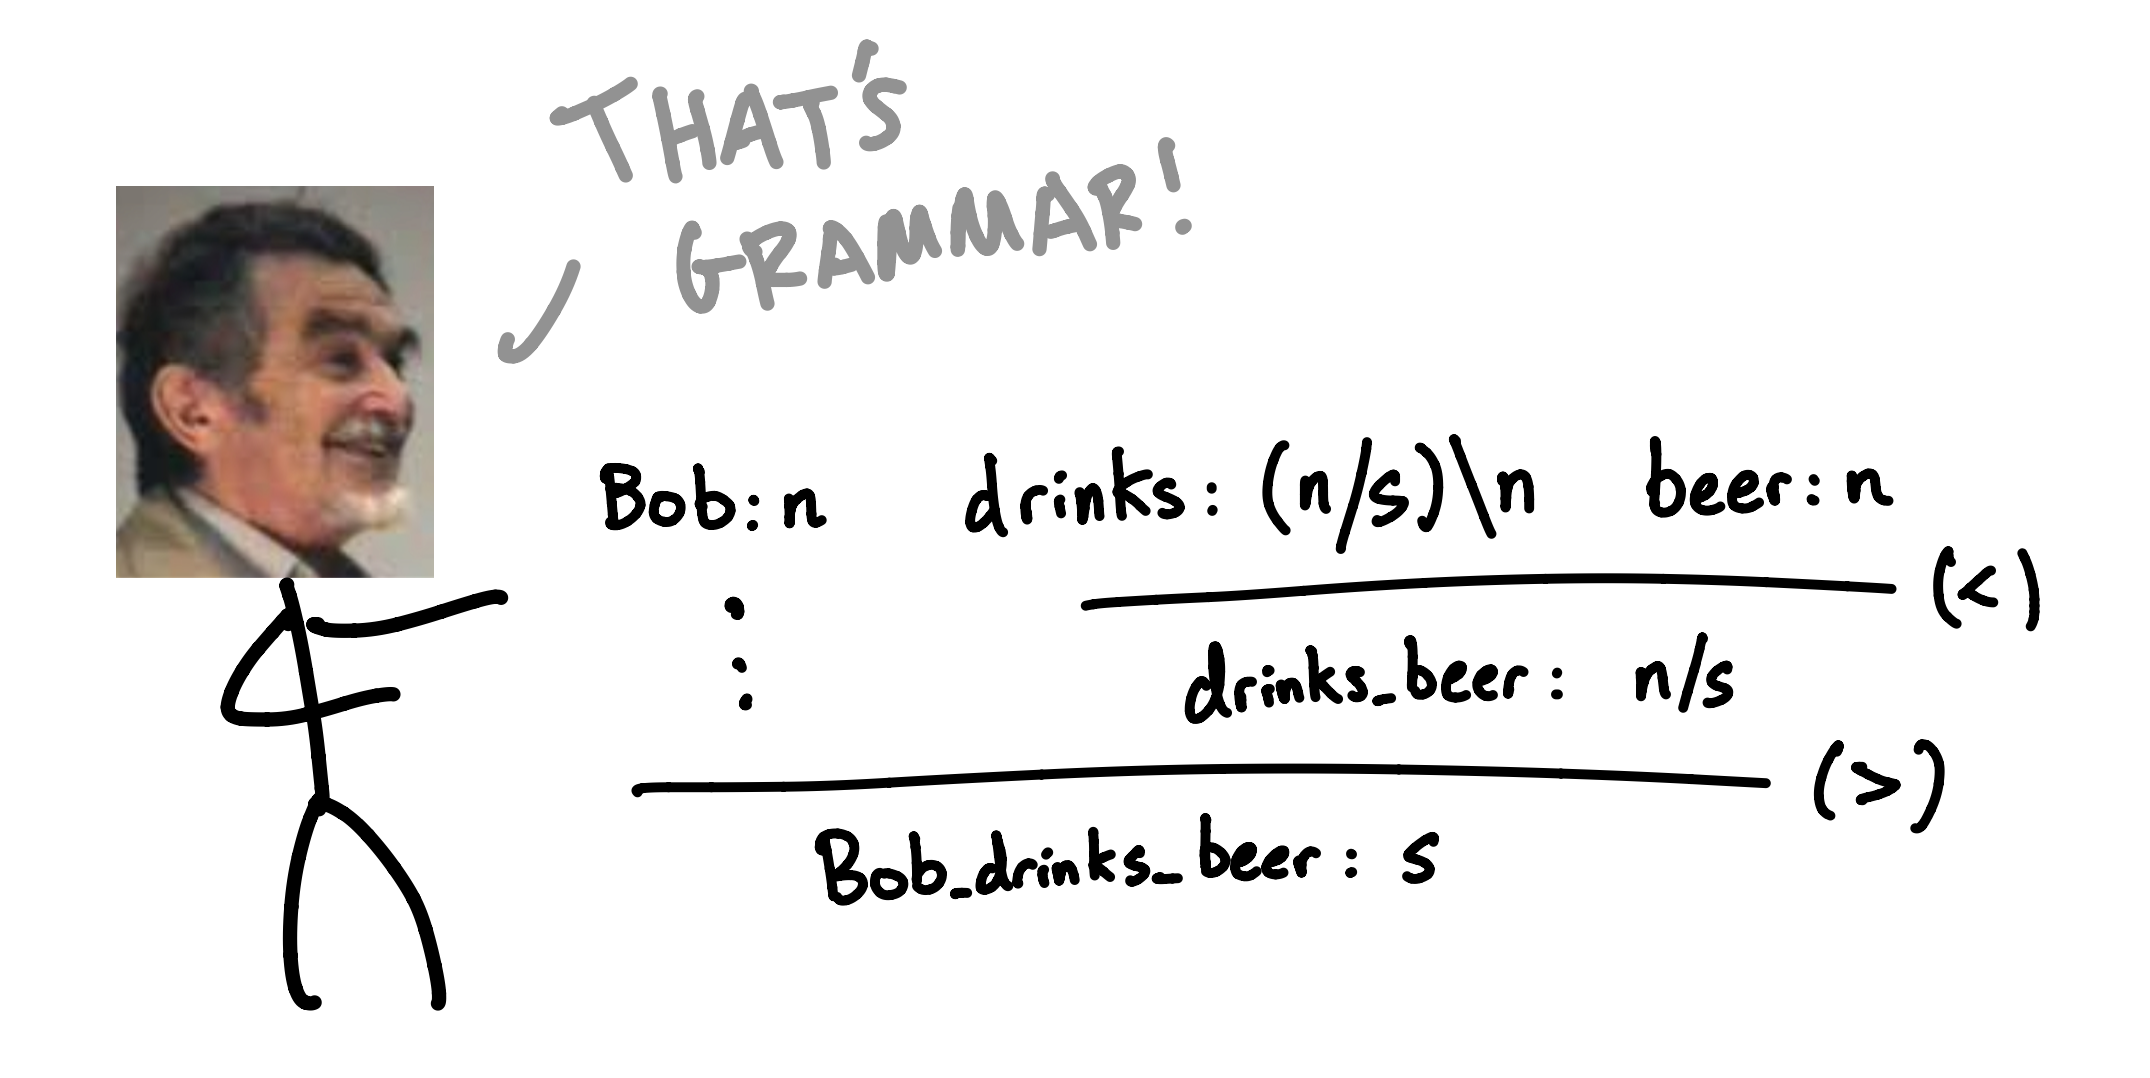
\includegraphics{figures/cartoons/lambek1}}
\caption{In English, we may consider a noun to have type $n$, and a transitive verb $(n/s)\setminus n$, to yield a well-formedness proof of \texttt{Bob drinks beer}. The type formation rules for such a grammar are intuitive. Apart from a stock of basic types $\mathbb{B}$ that contains special final types to indicate sentences, we have two type formation operators $(-/=)$ and $(- \setminus =)$, which along with their elimination rules establish a requirement that grammatical categories require other grammatical categories to their left or right. This is the essence of Lambek's calculi \textbf{NL} and \textbf{L}. CCGs keep the same minimal type-formations, but include extra sequent rules such as type-raising and cross-composition.}
\end{figure}

\begin{figure}[h!]
\centering
\scalebox{1}{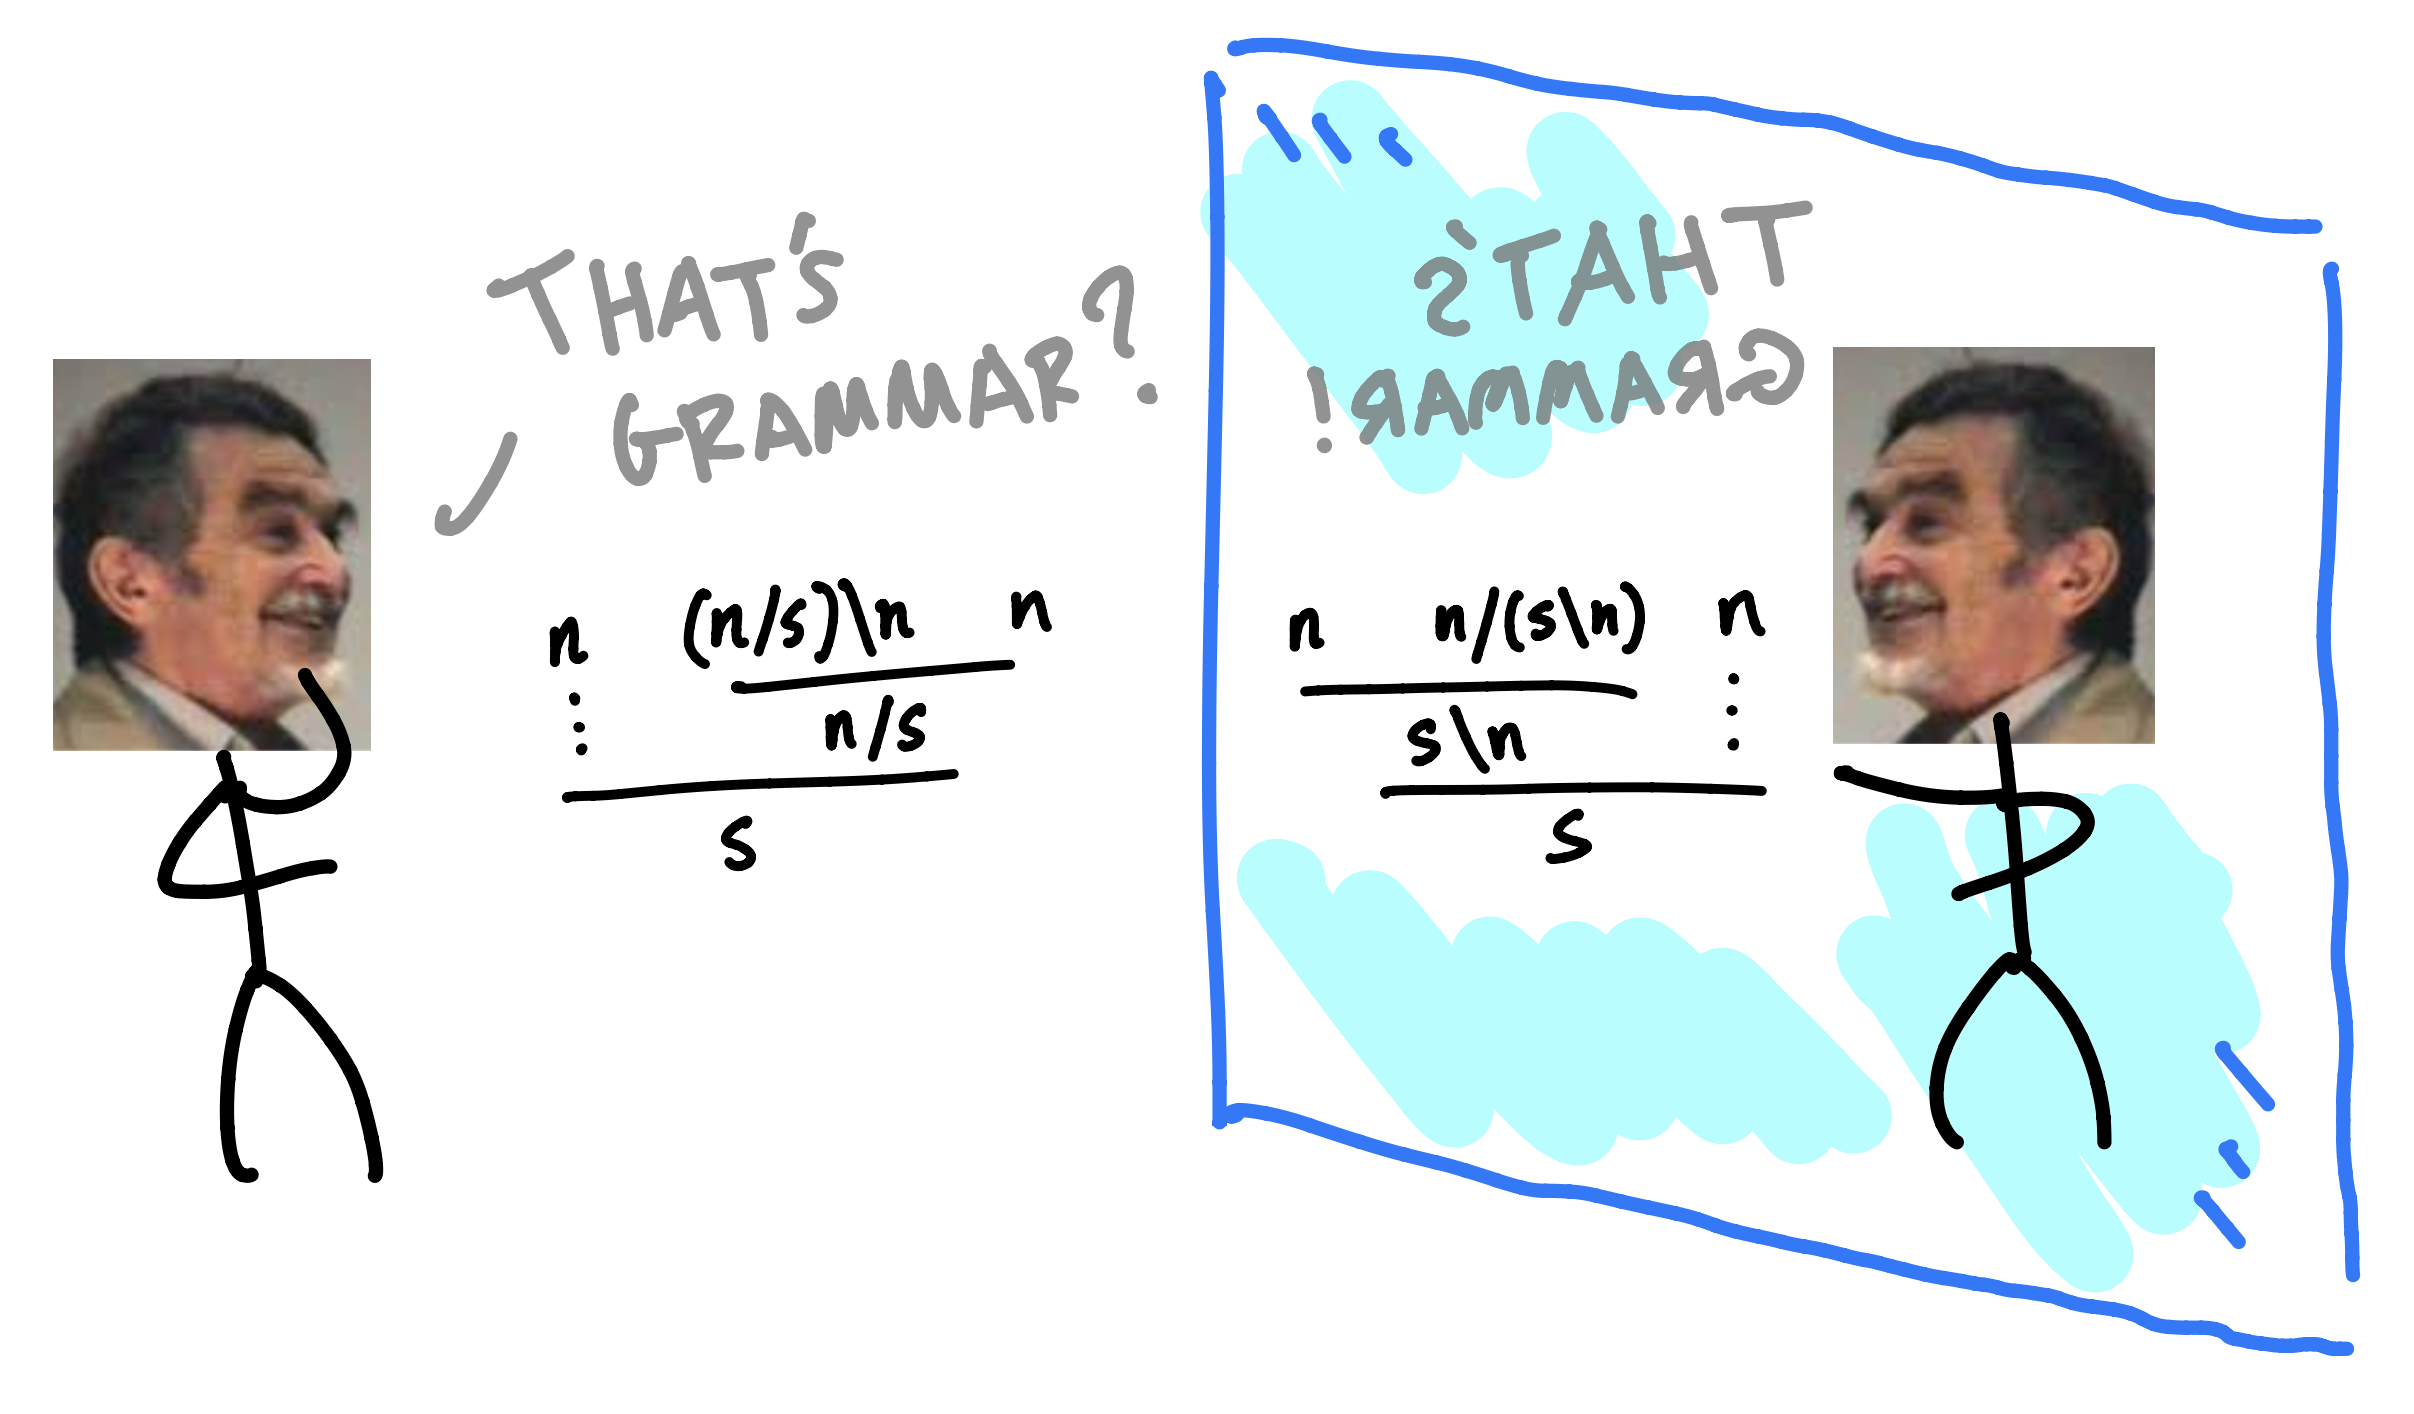
\includegraphics{figures/cartoons/lambek2}}
\caption{We can notice an asymmetry in the above formulation when we examine the transitive verb type $(n/s)\setminus n$ again; it asks first for a noun to the right, and then a noun to the left. We could just as well have asked for the nouns in the other order with the typing $(n/s)\setminus n$ and obtained all of the same proofs.}
\end{figure}

\begin{figure}[h!]
\centering
\scalebox{1}{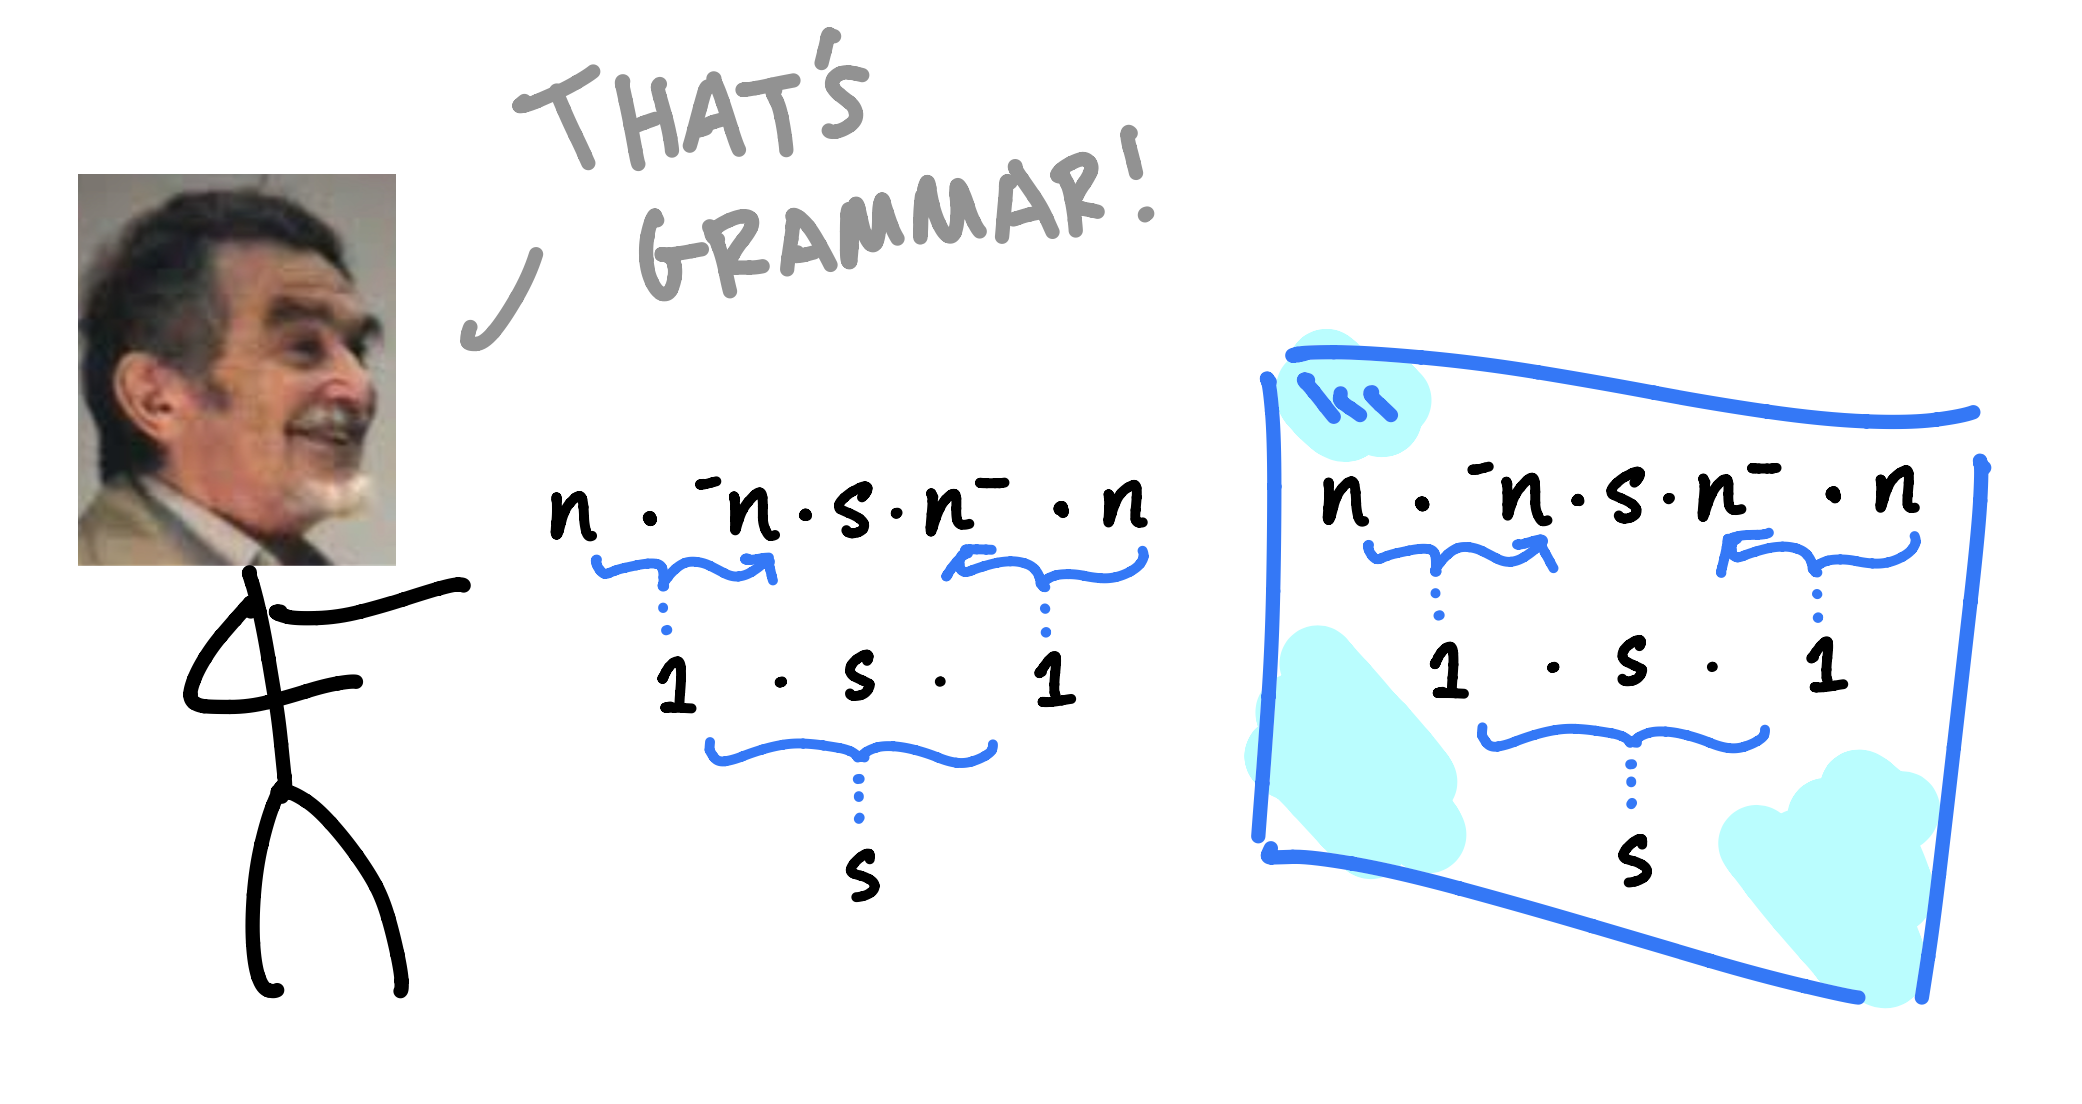
\includegraphics{figures/cartoons/lambek3}}
\caption{To eliminate this asymmetry, Lambek devised pregroup grammars. Whereas a group is a monoid with inverses up to left- and right-multiplication, a pregroup weakens the requirement for inverses so that all elements have distinct left- and right- inverses, denoted $x^{-1}$ and $^{-1}x$ respectively. Eliminating or introducing inverses is a non-identity relation on elements of the pregroup, so we have axioms of the form e.g. $x \cdot ^{-1}x \rightarrow 1 \rightarrow ^{1}x \cdot x$. In this formulation, denoting the multiplication with a dot, both $(n/s)\setminus n$ and $(n/s)\setminus n$ become $^{-1}n \cdot s \cdot n^{-1}$, which just wants a noun to the left and a noun to the right in whatever order to eliminate the flanking inverses to reveal the embedded sentence type. Now we can obtain the same proof of correctness as a series of algebraic reductions.

\begin{align*}
& &n \cdot (^{-1}n \cdot s \cdot n^{-1}) \cdot n\\
&\rightarrow &(n \cdot ^{-1}n) \cdot s \cdot (n^{-1} \cdot n)\\
&\rightarrow & 1 \cdot s \cdot 1\\
&\rightarrow & s
\end{align*}
}
\end{figure}
\clearpage

\subsection{Coecke's Composition}

\begin{figure}[h!]
\centering
\scalebox{0.9}{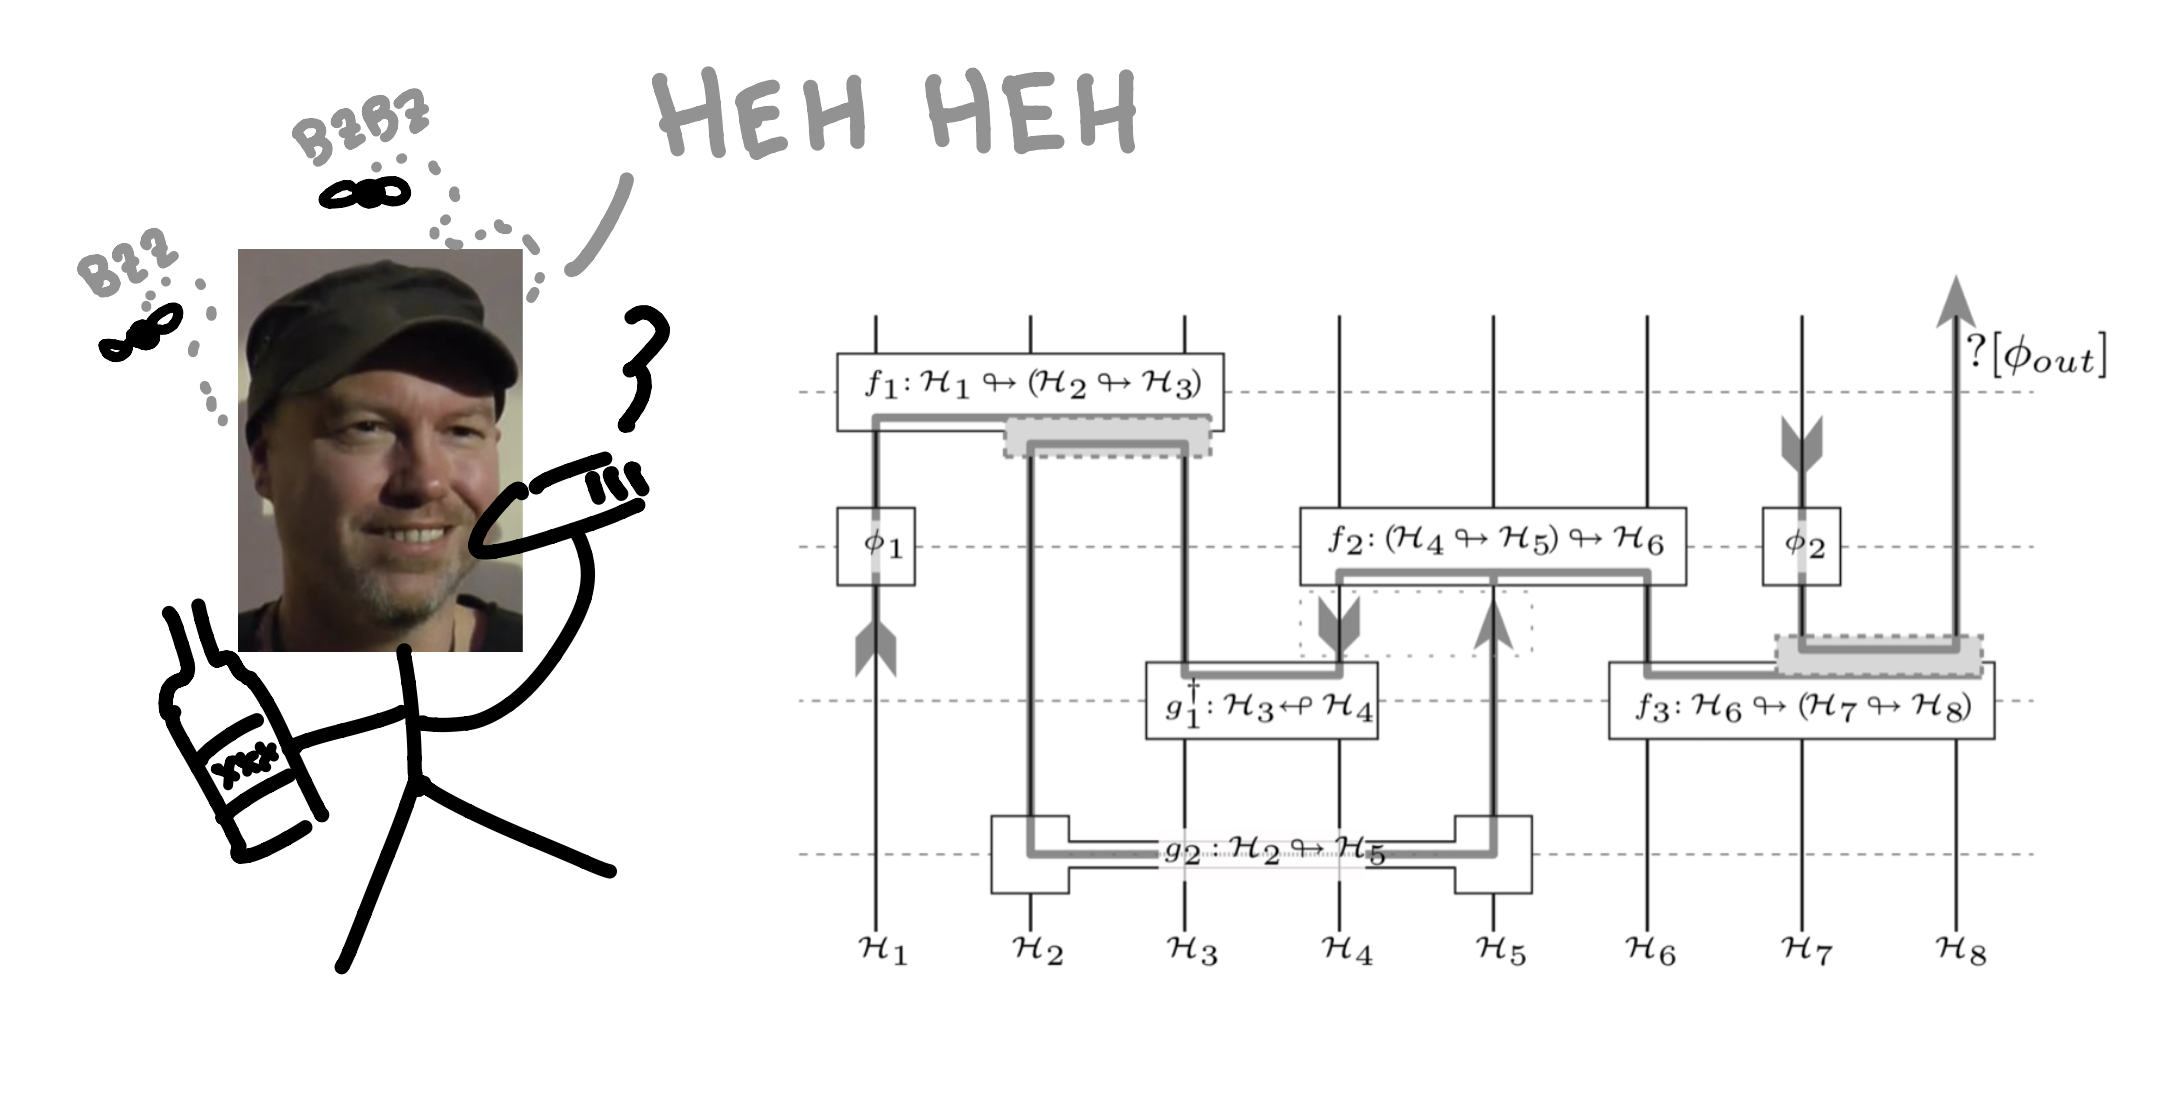
\includegraphics{figures/cartoons/bob1}}
\caption{Meanwhile, an underground grunge vagabond moonlighting as a quantum physicist moonlighting as a computer scientist was causing a shortage of cigars and whiskey in a small English town. He noticed a funny thing about the composition of multiple non-destructive measurements of a quantum system, which was that information could be carried, or flow, between them. So he wrote a paper \bR invitationtoquantum \e, which contained informal diagrams that looked like this.}
\end{figure}

\begin{figure}[h!]
\centering
\scalebox{0.9}{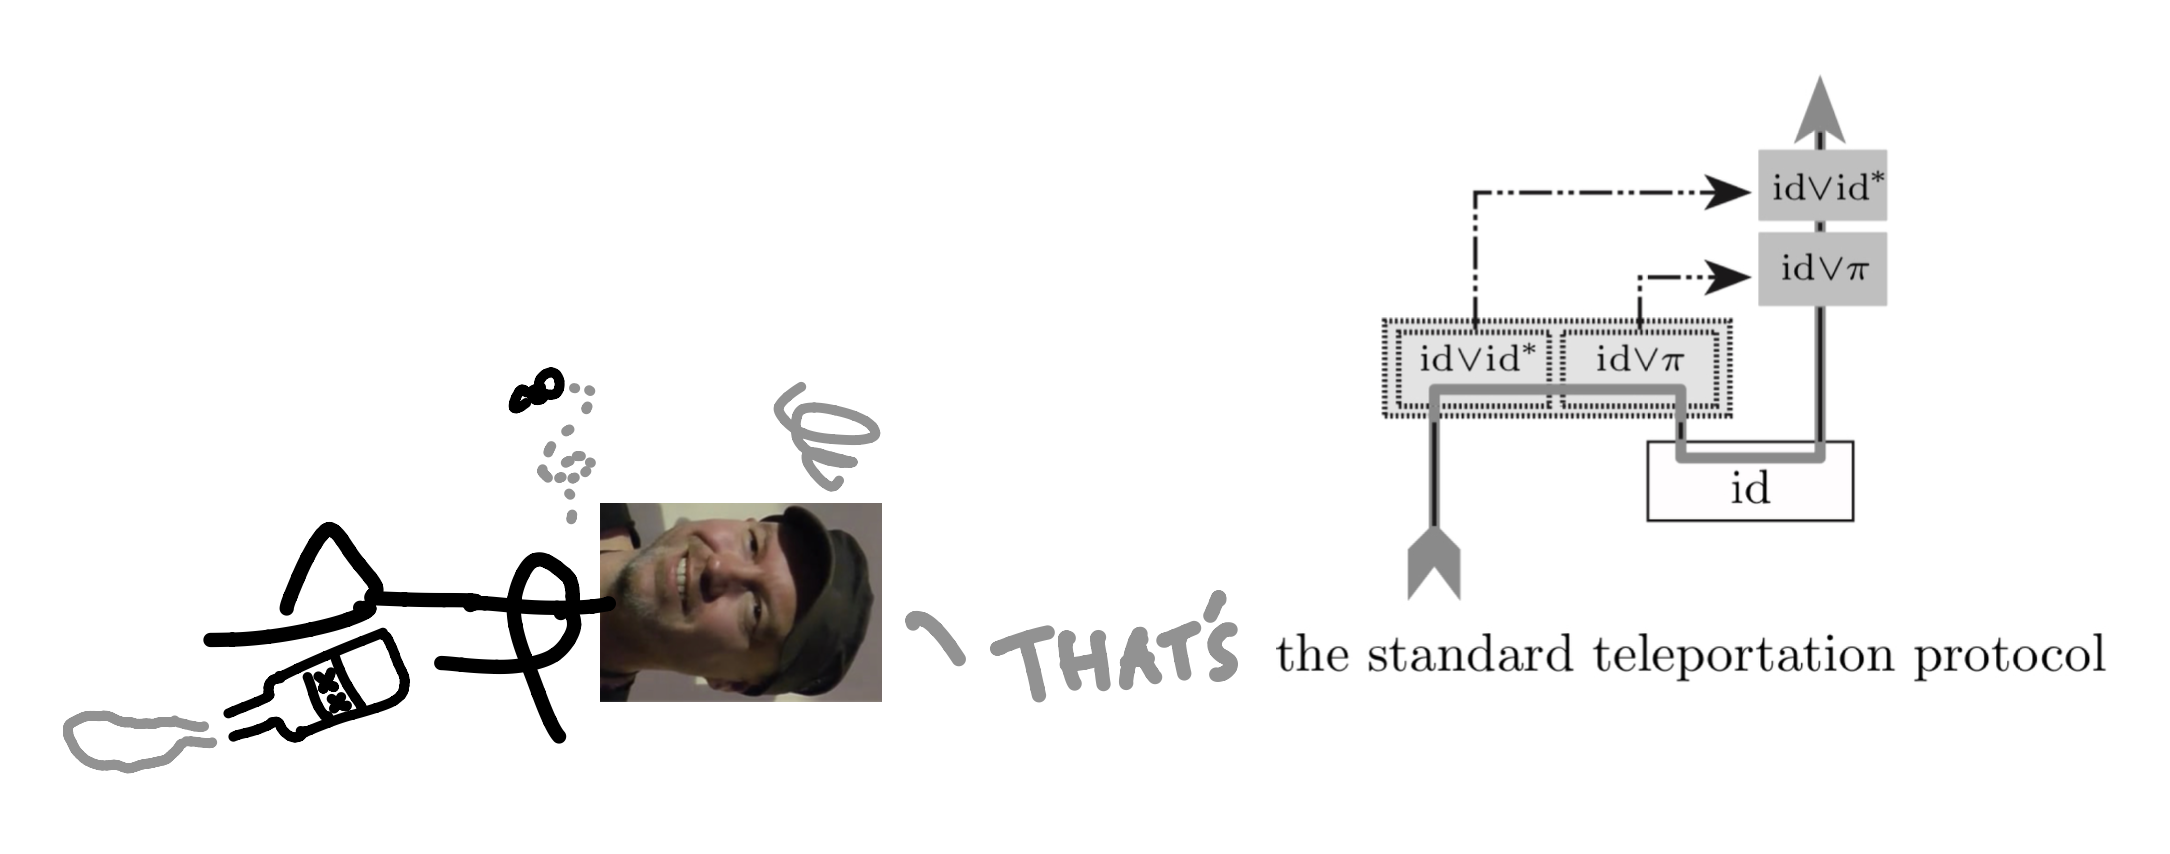
\includegraphics{figures/cartoons/bob2}}
\caption{There were two impressive things about these diagrams. First, the effects such as transparencies for text boxes and curved serifs for angled arrows give a modern feel, but they were done manually in macdraw, the diagrammatic equivalent of sticks and stones. Second, though the diagrams were informal, they provided a way to visualise and reason about entanglement that was impossible by staring at the equivalent matrix formulation of the same composite operator. The most important diagram for our story was this one, which captures the information flow of quantum teleportation.}
\end{figure}
\clearpage

\subsection{Categorical quantum mechanics}

\begin{figure}[h!]
\centering
\scalebox{1}{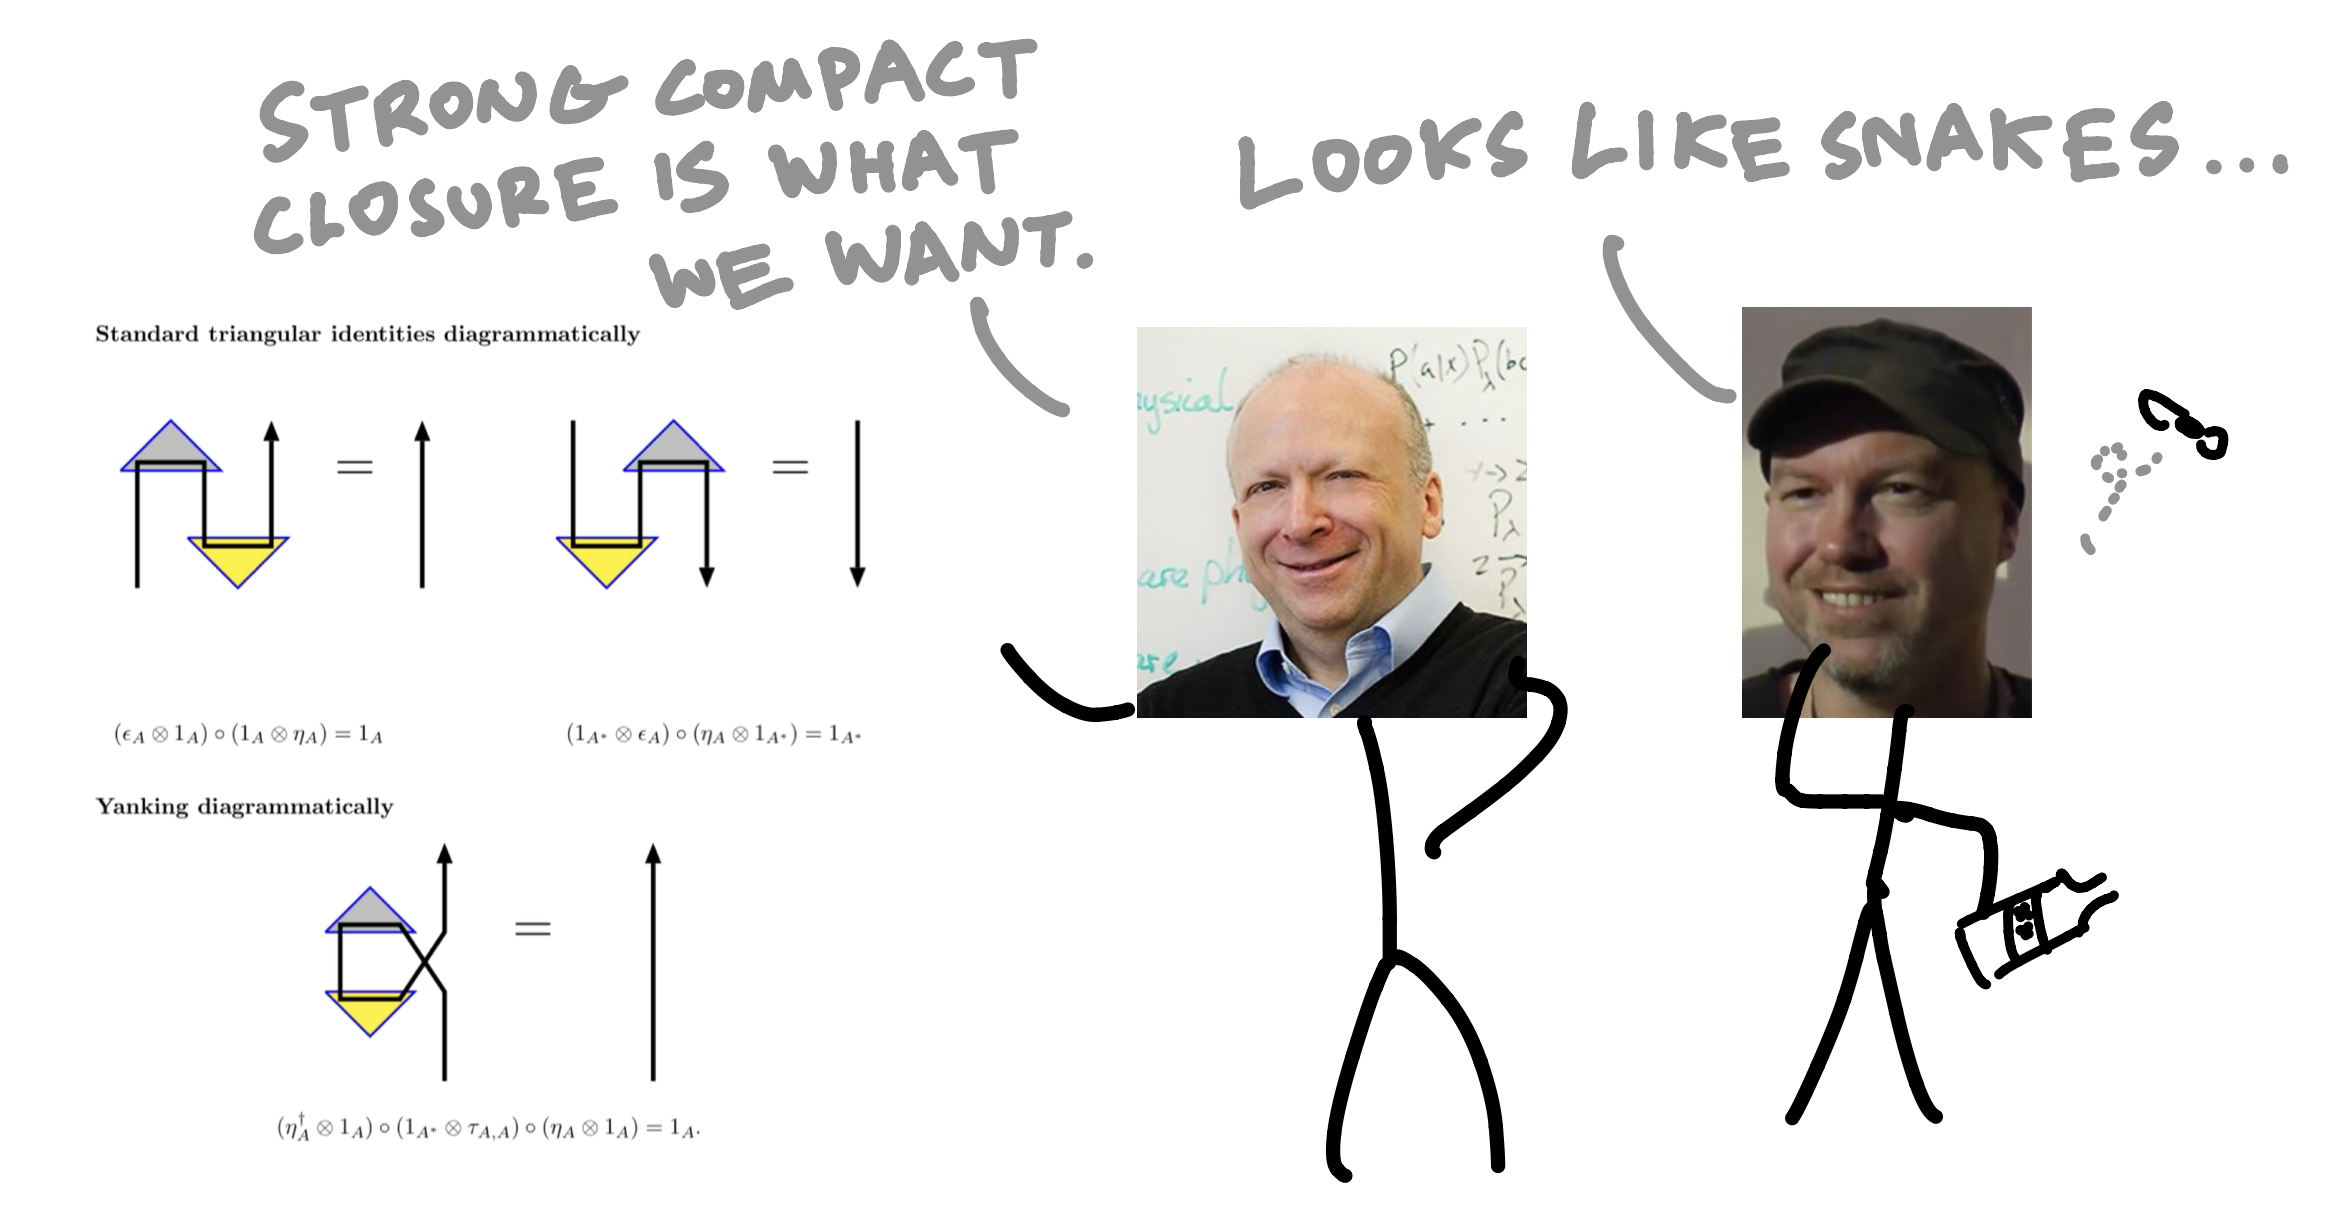
\includegraphics{figures/cartoons/samson}}
\caption{Category theorists and physicists such as Abramsky and Baez were excited about these diagrams, which looked like string diagrams waiting to be made formal. The graphical cups and caps in the important diagram were determined to correspond to a special form of symmetric monoidal closed category called strong compact closed.}
\end{figure}

\begin{figure}[h!]
\centering
\scalebox{1}{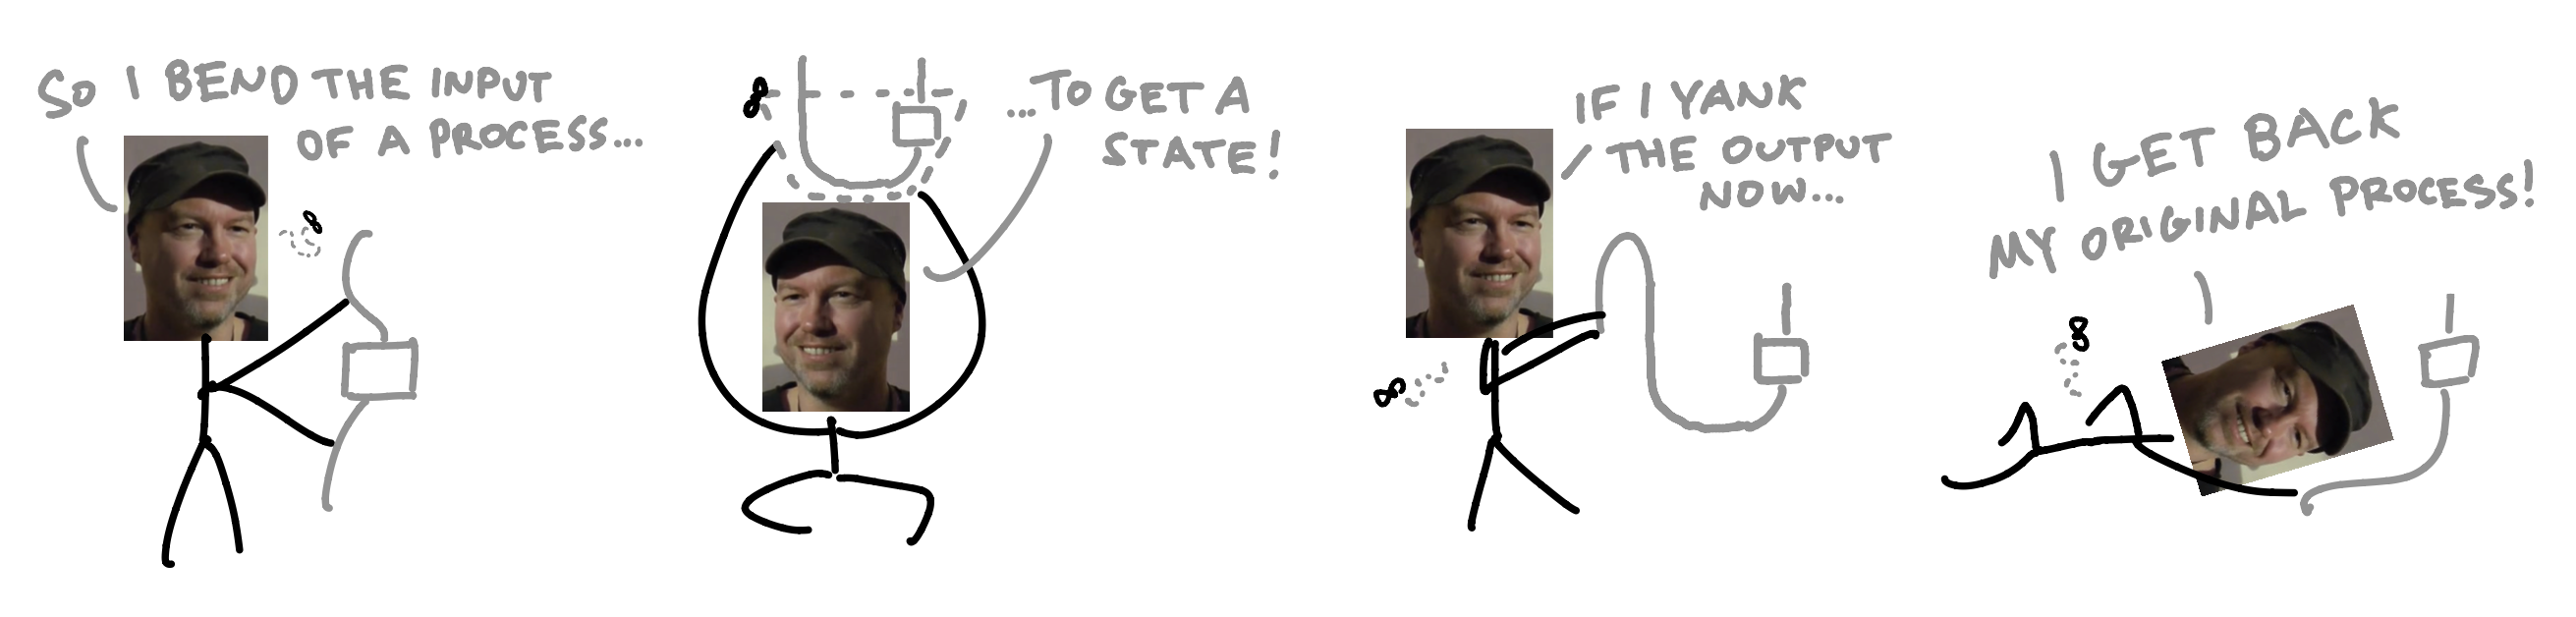
\includegraphics{figures/cartoons/cjiso}}
\caption{Diagrammatically, reasoning in a strongly compact closed category amounts to ignoring the usual requirement of processiveness and forgetting the distinction between inputs and outputs, so that "future" outputs could curl back and be "past" inputs. This formulation also gave insight into the structure of quantum mechanics. For example, the process-state duality of strong compact closure manifested as the Choi–Jamiołkowski isomorphism.}
\end{figure}

\begin{figure}[h!]
\centering
\scalebox{1}{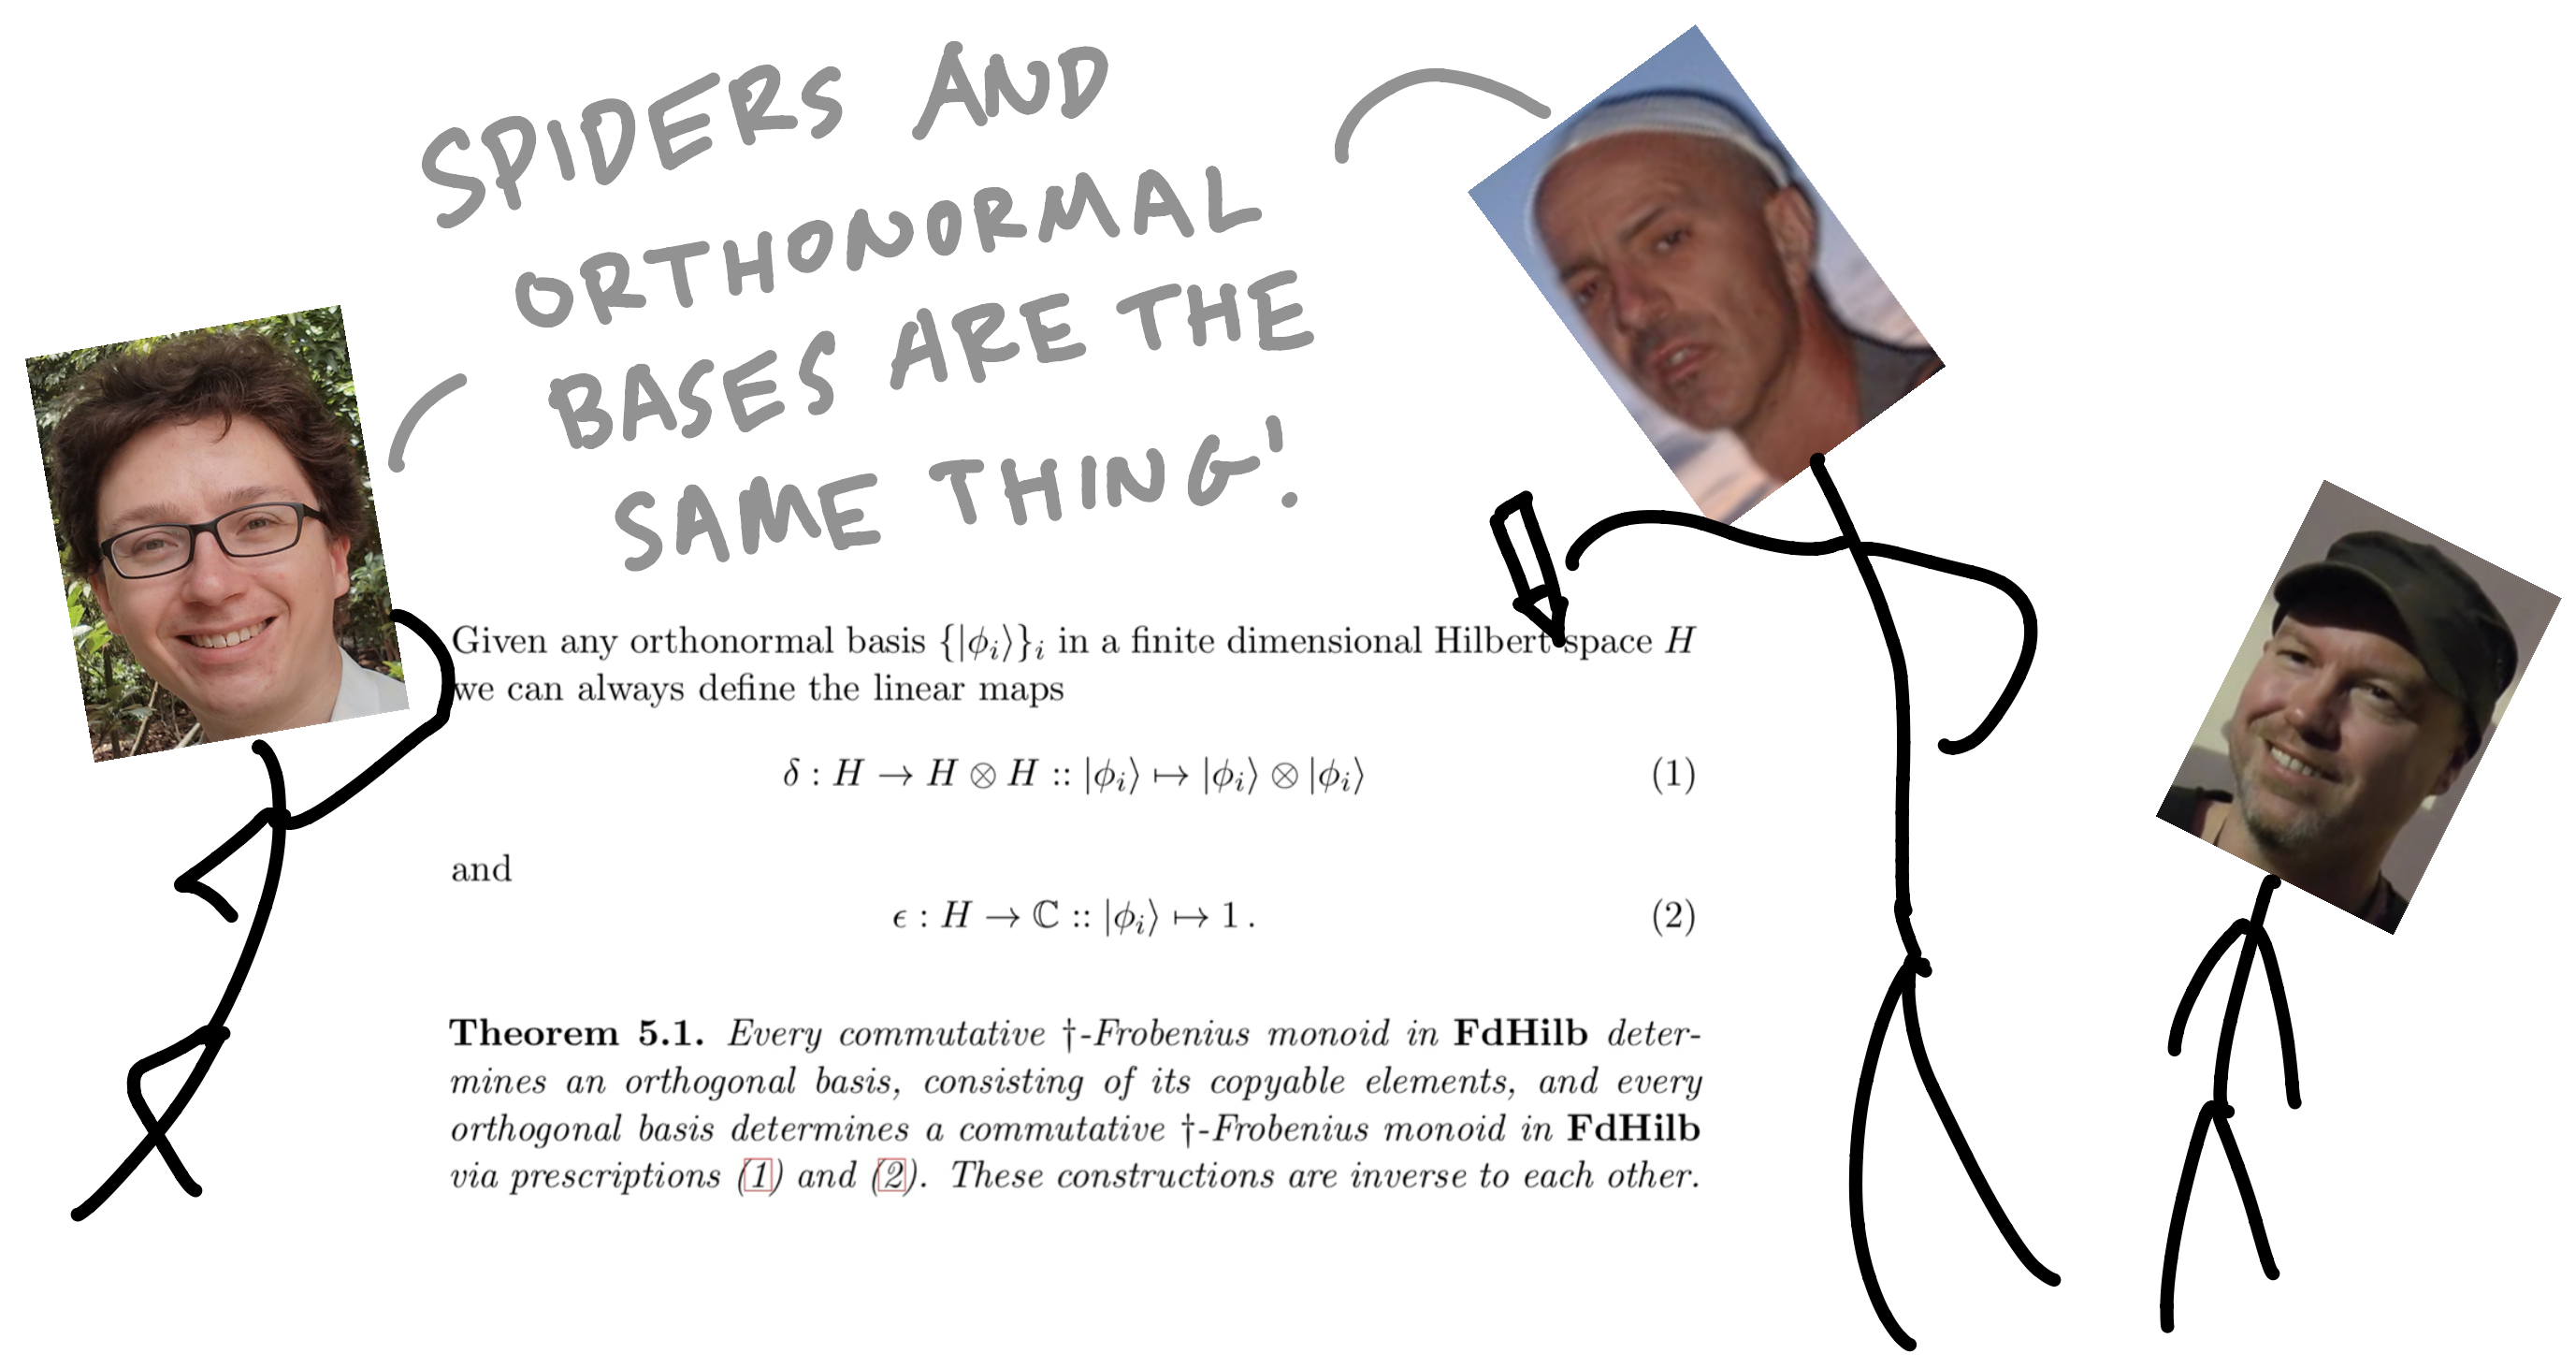
\includegraphics{figures/cartoons/spiders}}
\caption{However, dealing with superpositions necessitated using summation operators within diagrams, which is cumbersome to write especially when dealing with even theoretically simple Bell states. An elegant diagrammatic simplification arose with the observation that special-$\dagger$-frobenius algebras \bR classicquantumstruct \e, or spiders, correspond to choices of orthonormal bases \bR novelchar \e in \textbf{FdHilb}, the ambient setting of finite-dimensional hilbert spaces. Not only did this remove the need for summation operators, it also revealed that strong compact closure was a derived, rather than fundamental structure, since spiders induce compact closed structure.}
\end{figure}

\begin{figure}[h!]
\centering
\scalebox{1}{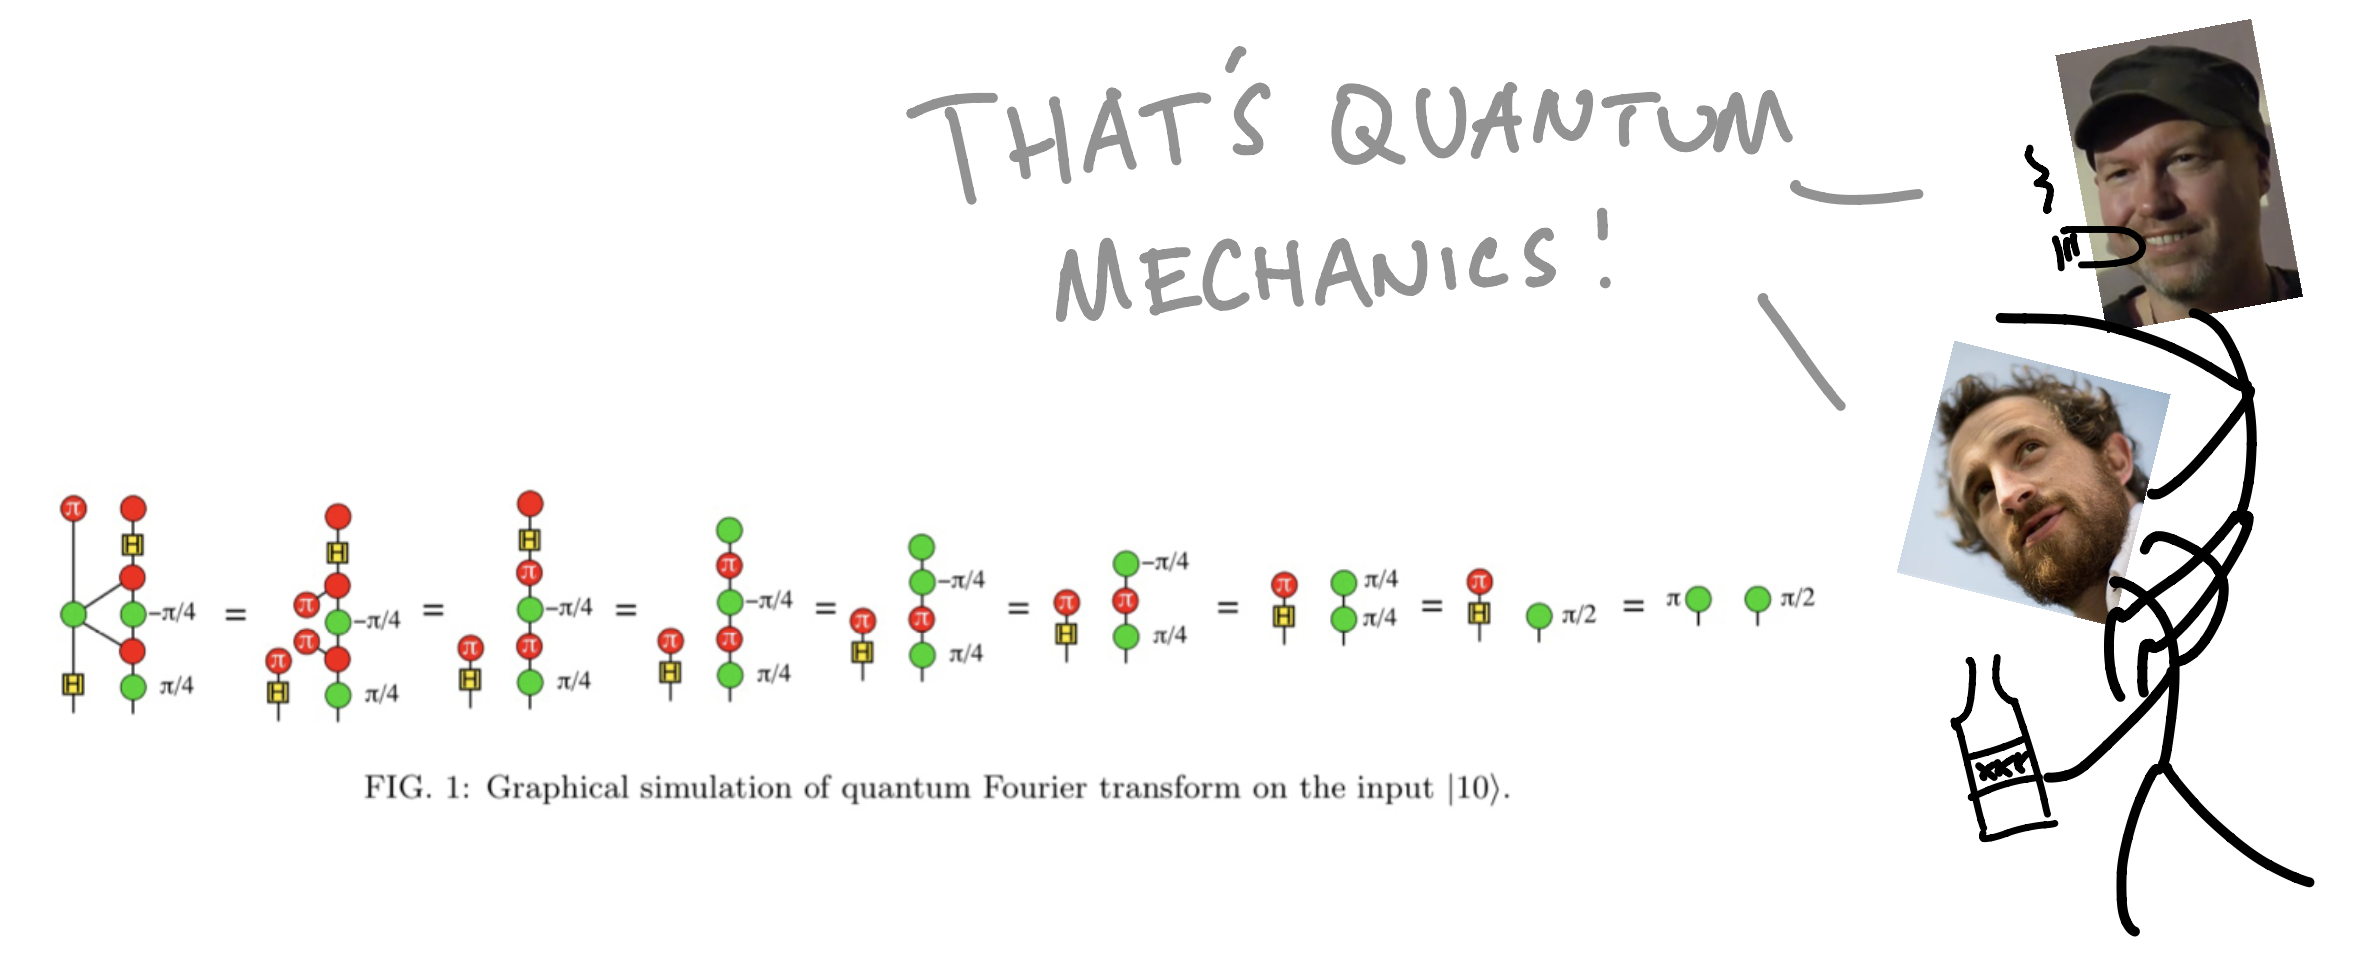
\includegraphics{figures/cartoons/ross}}
\caption{And so the stage was set for a purely diagrammatic treatment of ZX quantum mechanics. The story of ZX diverges away from our interest, so I will summarise what happened afterwards. In no particular order, the development of ZX went on to accommodate a third axis of measurement to yield a ZXW calculus \bR CITE \e, the systems were proven to be complete \bR CITES \e, there are at the time of writing two expository books \bR CITES \e, and ZX-variants are becoming an industry standard for quantum circuit specification and rewriting \bR CITE \e.}
\end{figure}
\clearpage

\subsection{Enter computational linguistics}

\begin{figure}[h!]
\centering
\scalebox{1}{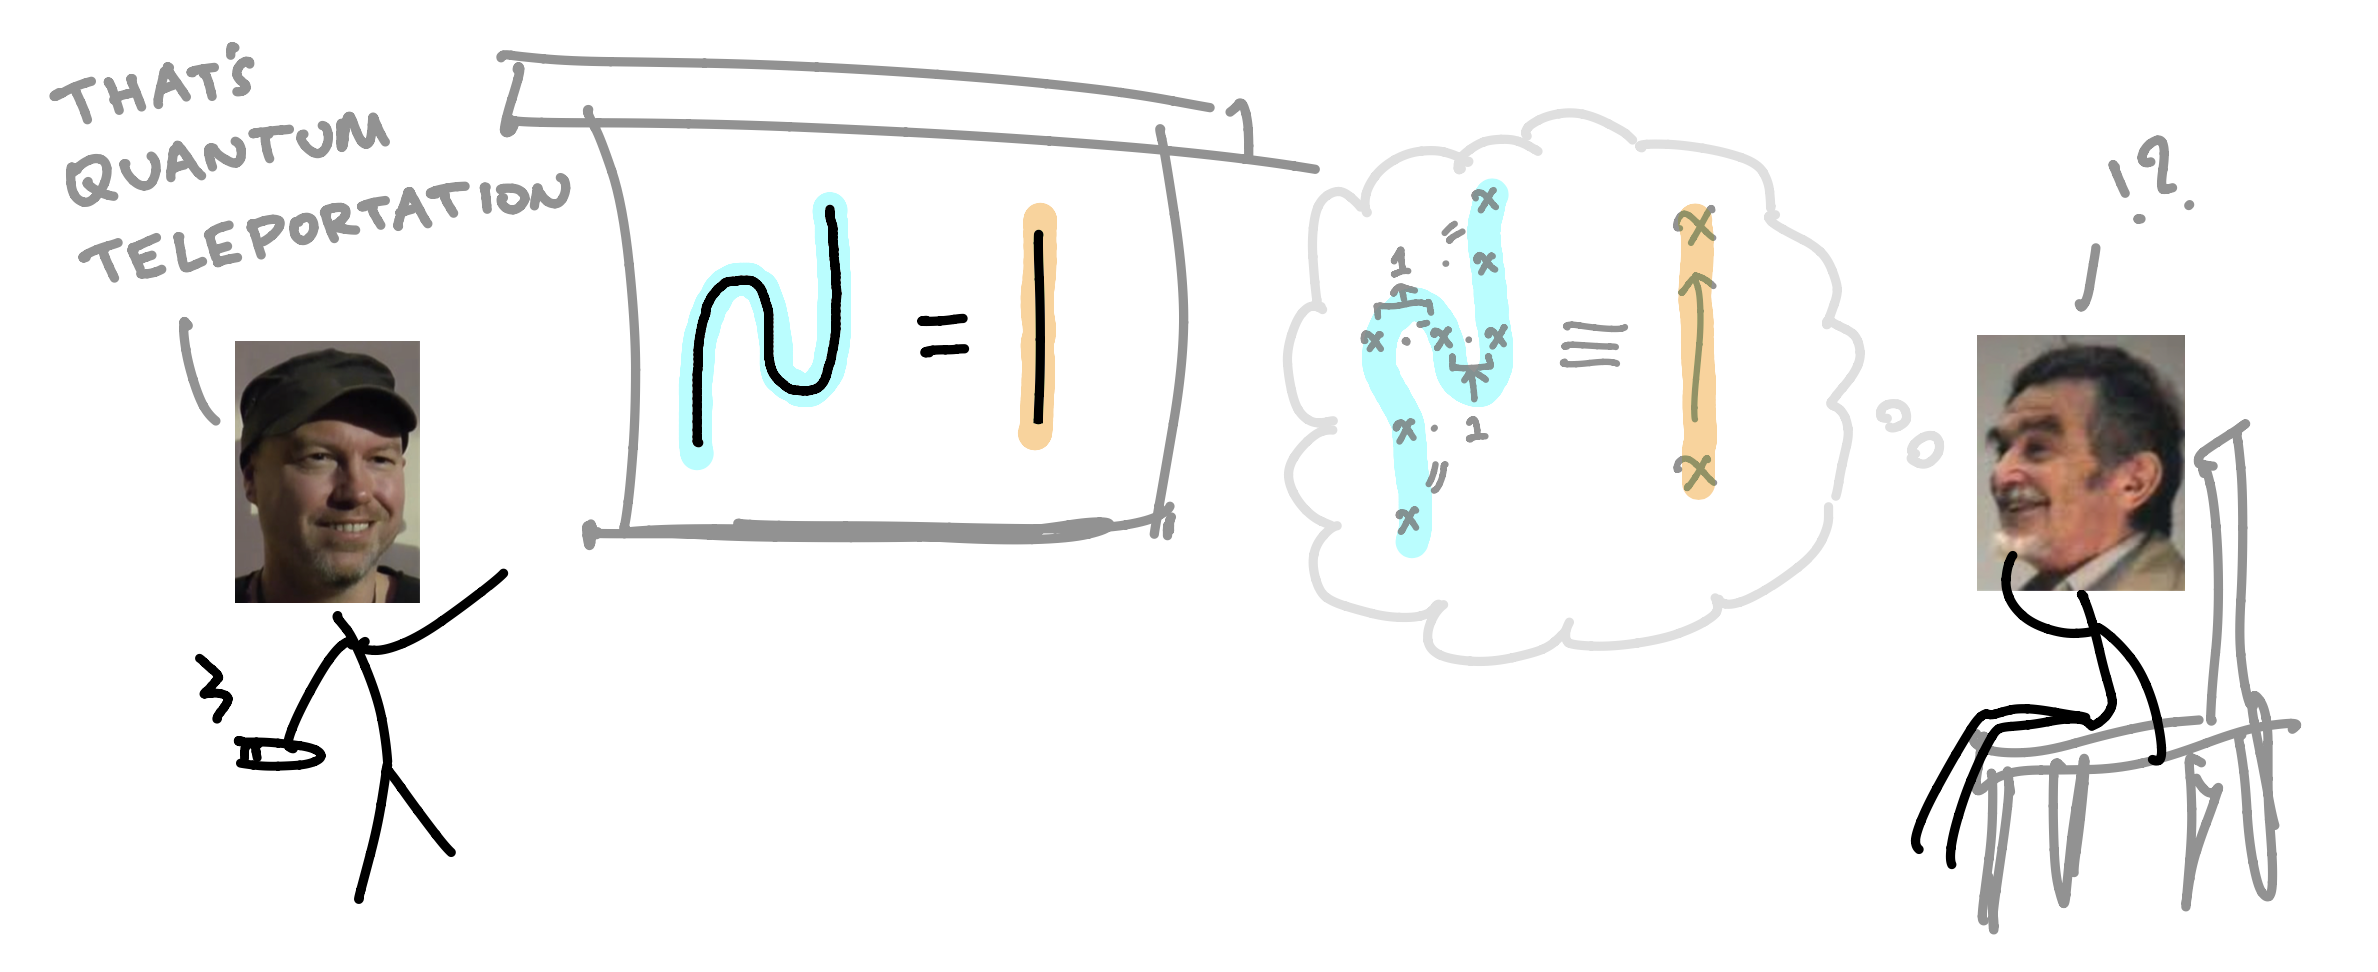
\includegraphics{figures/cartoons/boblambek1}}
\caption{Somewhere in Canada at the turn of the millenium, Bob met Jim, who saw something familiar about the diagram for quantum teleportation. The snake equation for compact closure looked a lot like the categorified version of introducing and eliminating pregroup types.
}
\end{figure}

\begin{figure}[h!]
\centering
\scalebox{1}{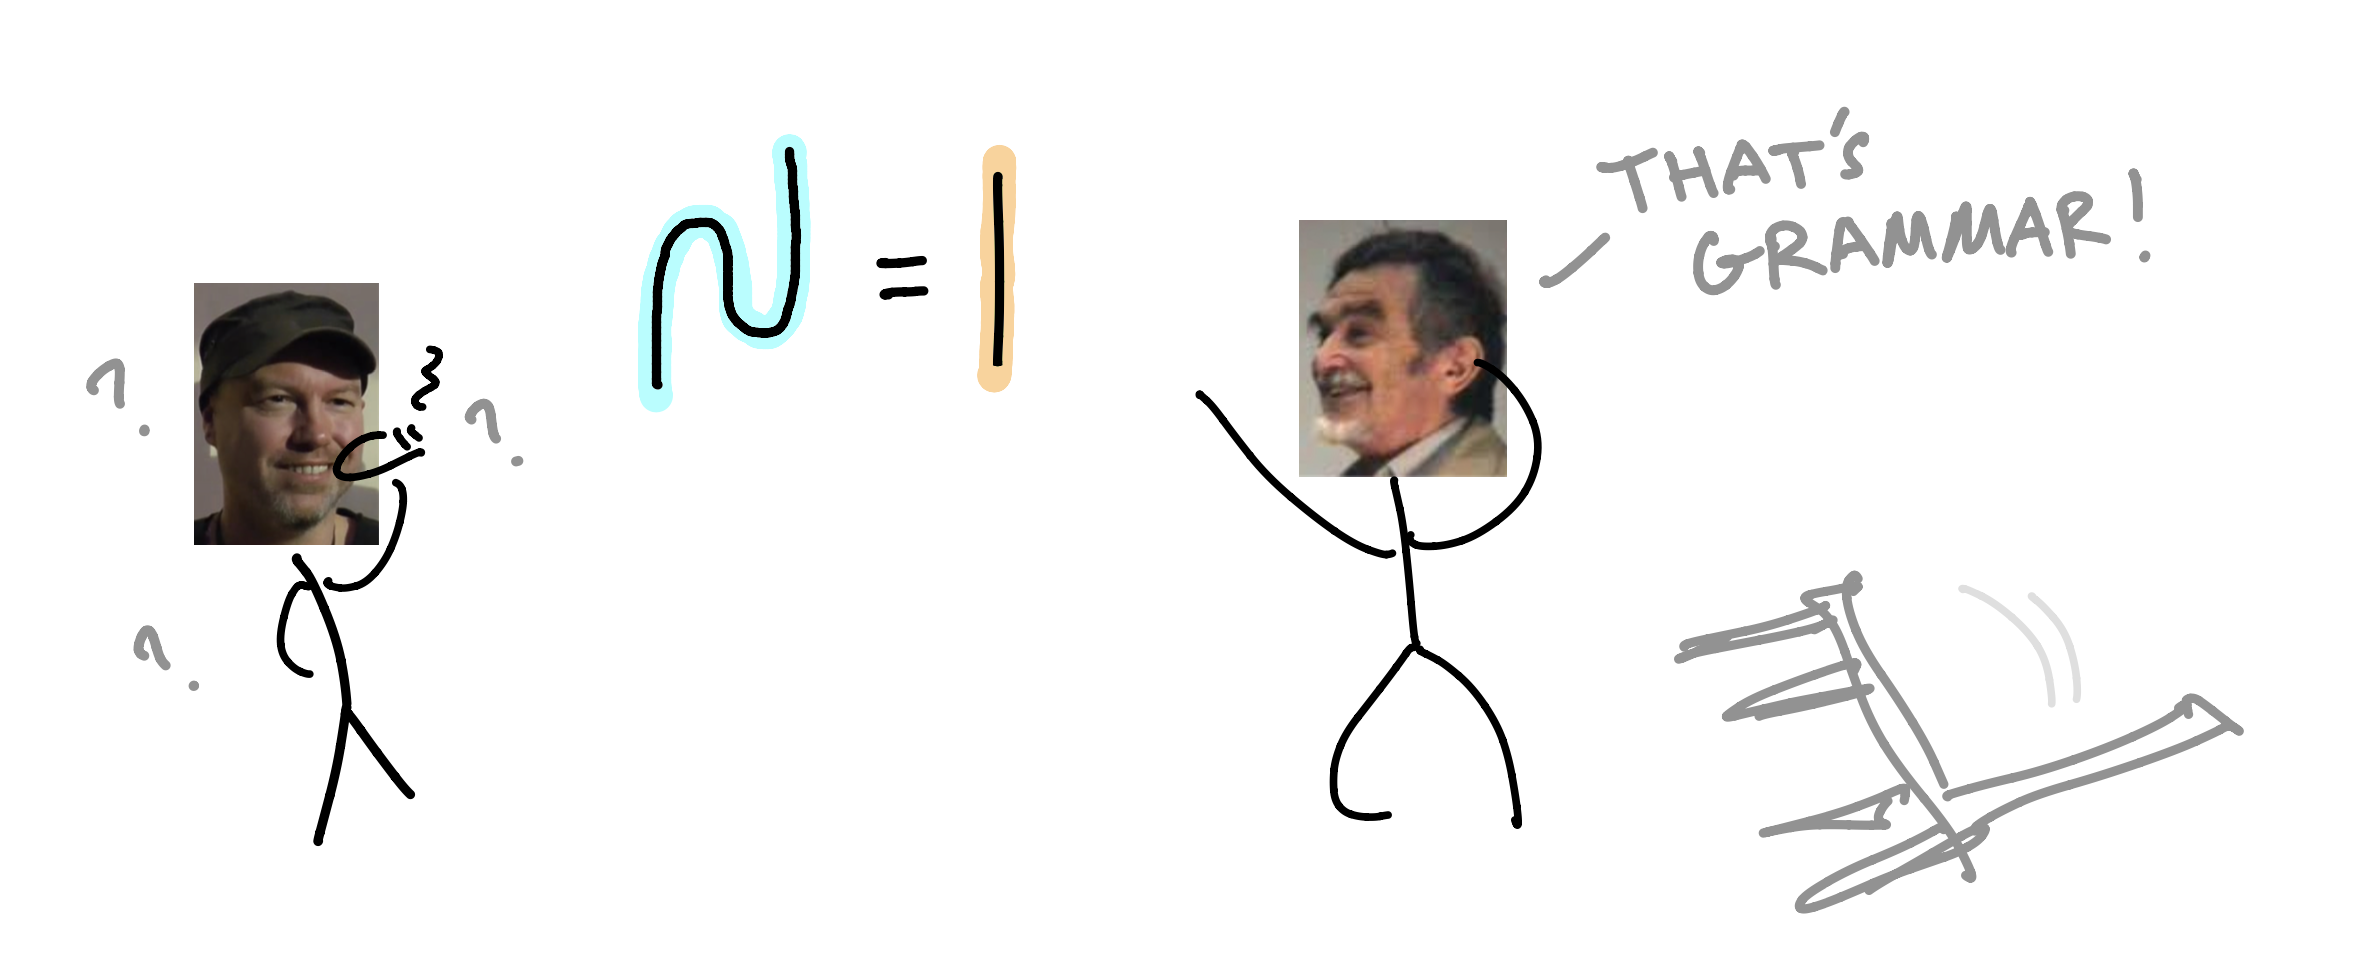
\includegraphics{figures/cartoons/boblambek2}}
\caption{Bob and Jim's meeting put the adjectives \emph{compositional} and \emph{categorical} on the same table, but the cake wasn't ready. Two more actors Steve and Mehrnoosh were required to introduce \emph{distributional}, which refers to Firth's maxim \bR CITE \e "you shall know a word by the company it keeps". In its modern incarnation, this refers generally to vector-based semantics for words, where it is desirable but not necessarily so (as in the case of generic latent space embeddings by an autoencoder) that proximity of vectors models semantic closeness.}
\end{figure}

\begin{figure}[h!]
\centering
\scalebox{1}{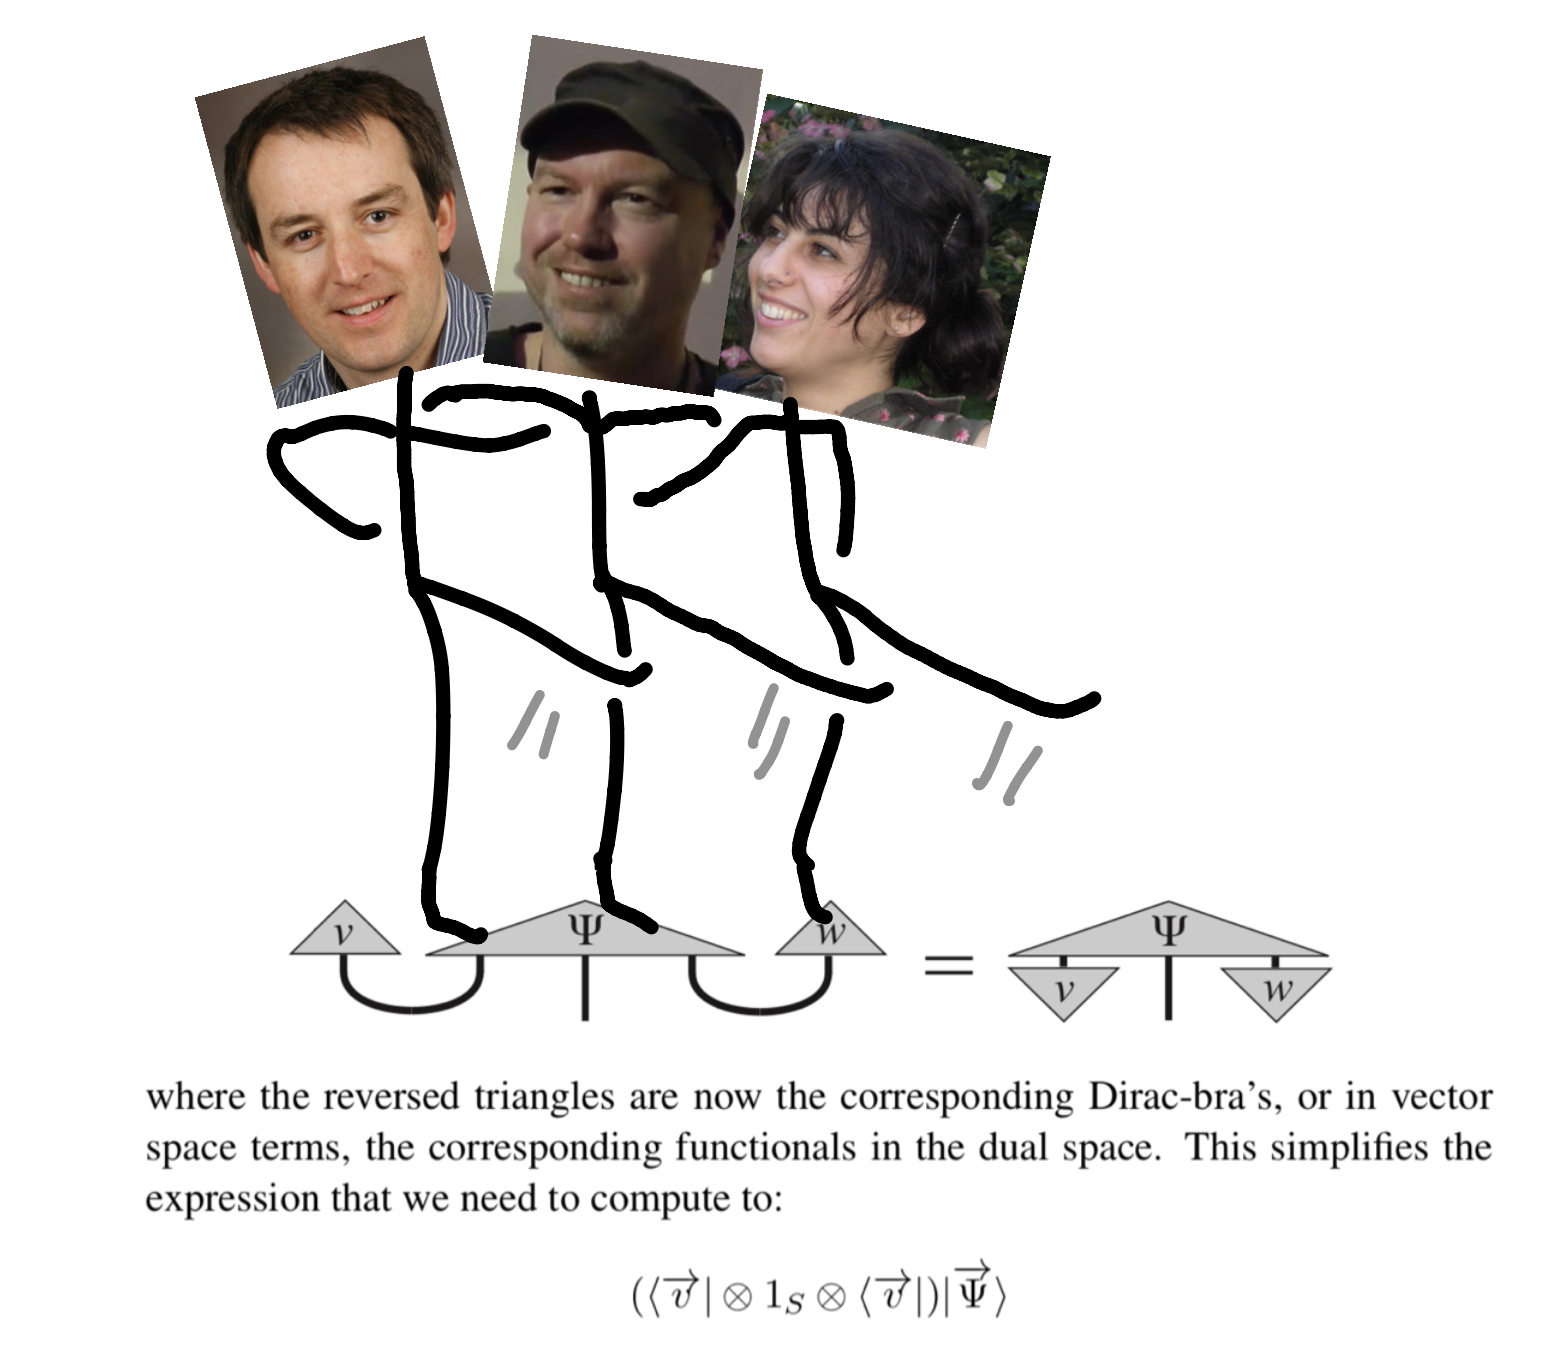
\includegraphics{figures/cartoons/disco1}}
\caption{Steve Clark was a professor in the computer science department at Oxford, and he was wondering how to compose vector-based semantic representations. Steve asked Bob, who realised suddenly what Jim was talking about. Mediated by the linguistic expertise of Mehrnoosh who was a postdoctoral researcher in Oxford at the time, pregroup diagrams were born. The basic types $n$ and $s$ are assigned finite-dimensional vector spaces, concatenation of types the kronecker product $\otimes$, and by the isomorphism of dual spaces in finite dimensions there is no need to keep track of the left- and right- inverse data. Words become vectors, and pregroup reductions become bell-states, or bell-measurements, depending on whether one reads top-down or bottom-up. There was simply no other game in town for an approach to computational linguistics that combined linguistic compositionality with distributional representations.}
\end{figure}

\begin{figure}[h!]
\centering
\scalebox{1}{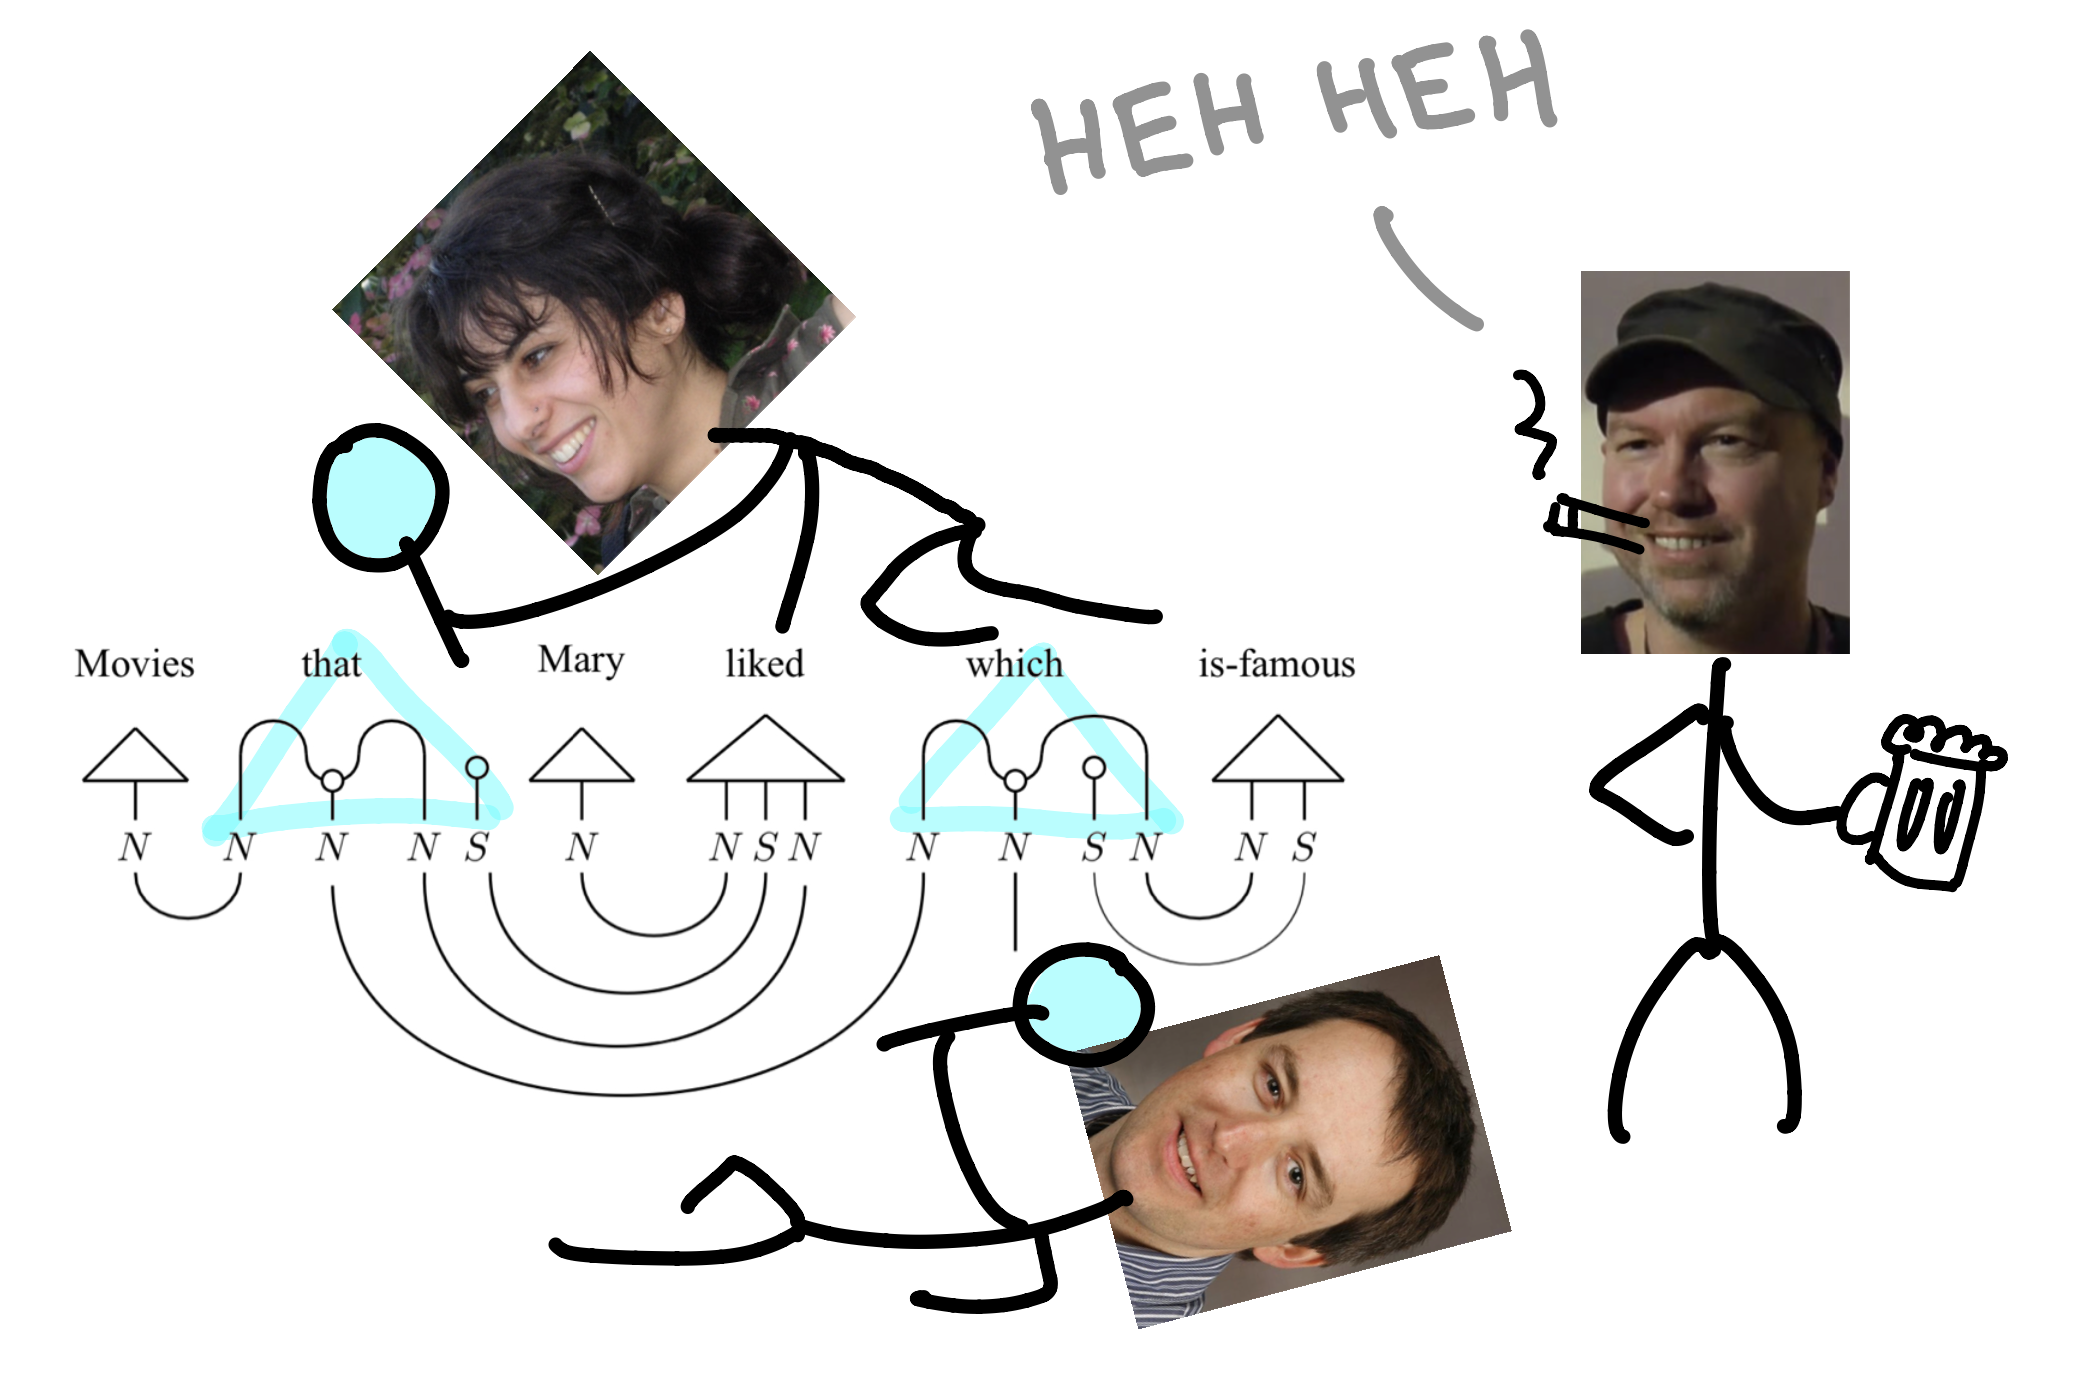
\includegraphics{figures/cartoons/disco2}}
\caption{In \emph{the frobenius anatomy of relative pronouns}\bR CITE \e, the trio realised that spiders could play the role of relative pronouns, which was genuinely novel linguistics. If one follows the noun-wire of "movies", one sees that by declaring the relative pronoun to be a vector made up of a particular bunch of spiders-as-multiwires, "movies" is copied to be related to the "liked" word, copied again by "which" to be related to the "is-famous" word, and a third time to act as the noun in the whole noun-phrase. This discovery clarified a value proposition: insights from quantum theory could be applied in the linguistic setting, and linguistics offered a novel use-case for quantum computers. For example, density matrices were used to model semantic ambiguity \bR CITE \e, and natural language experiments were performed on real quantum computeres \bR CITE \e.}
\end{figure}

\begin{figure}[h!]
\centering
\scalebox{1}{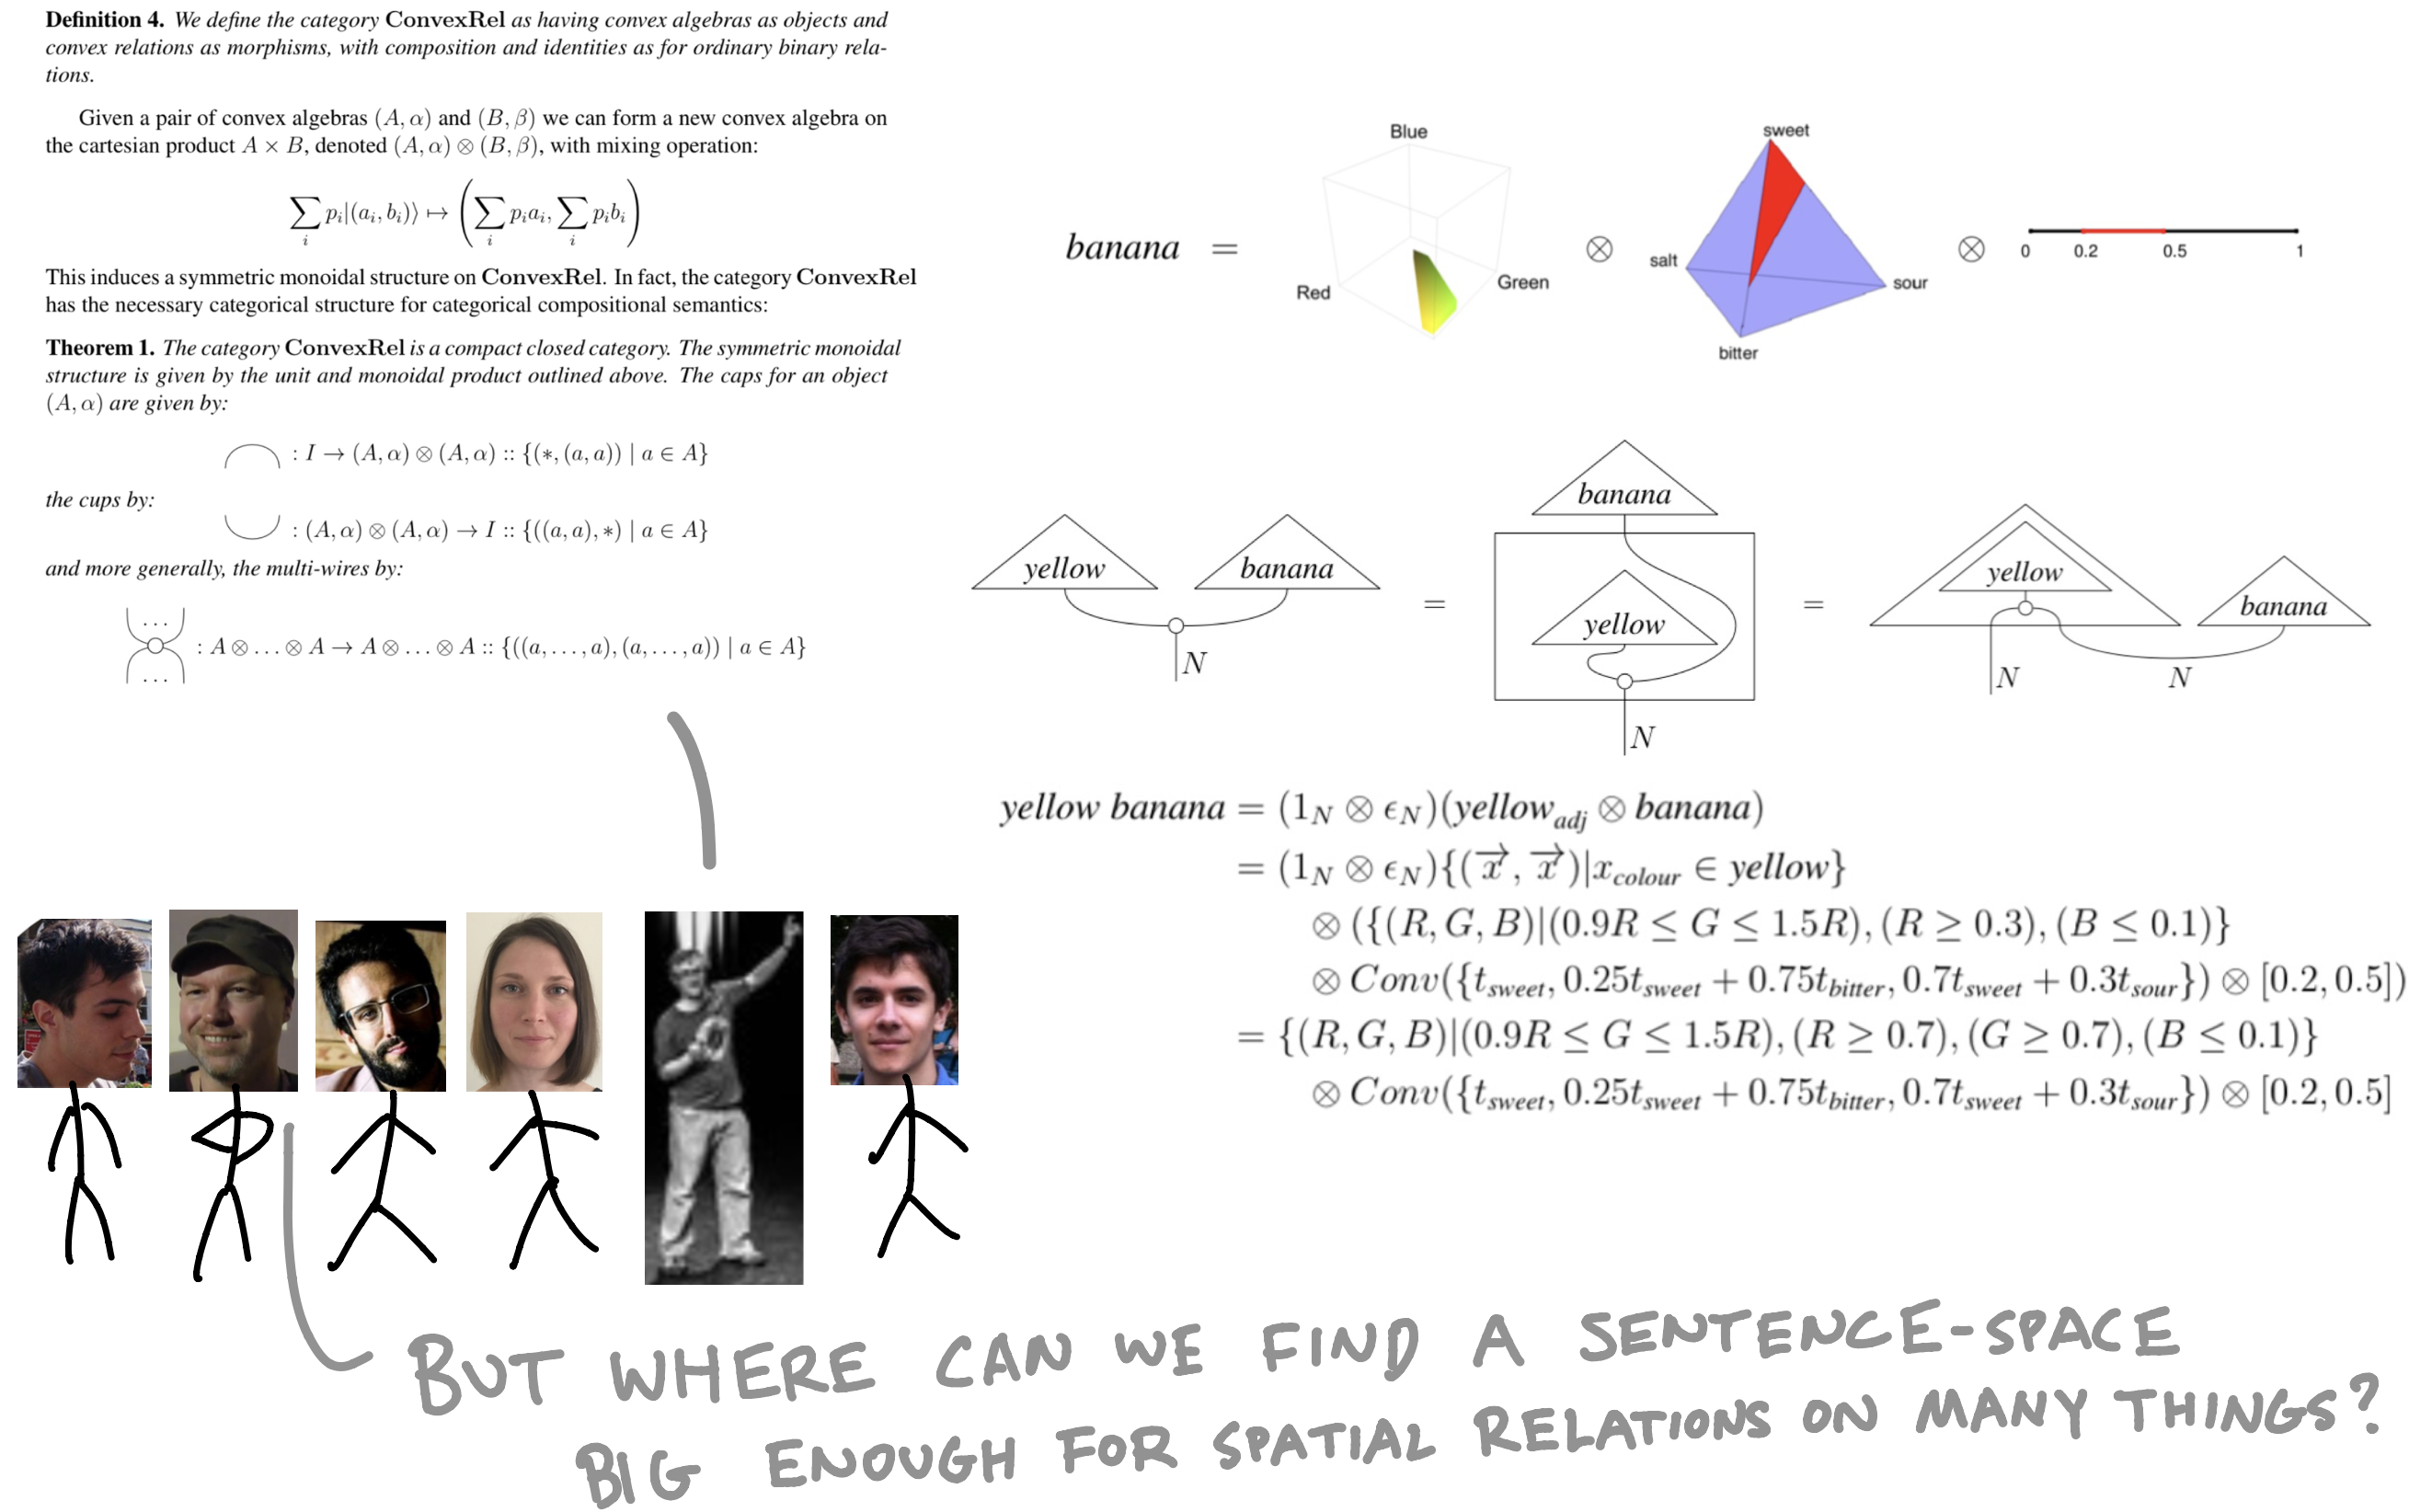
\includegraphics{figures/cartoons/disco3}}
\caption{Keeping the structure of the diagrams but seeking set-relational rather than vector-based semantics, a bridge was made between linguistics and cognitive science in \emph{interacting conceptual spaces I}\bR CITE \e. Briefly, G\"{a}rdenfors posits that spatial representations of concepts mediate raw sense data and symbolic representations -- e.g. red is a region in colourspace -- and moreover that concepts ought to be spatially convex -- e.g. mixing any two shades of red still gives red. This paper created a new point in the value proposition: that new mathematics would arise from investigating the linguistic-quantum bridge, e.g. generalised relations \bR CITE \e. Although labelled as if it is the first in a series, the paper never saw a sequel by the same title, blocked by an apparently simple but actually tricky theoretical problem. The problem is that while this convex-relational story worked for conceptual adjectives modifying a single noun such for "sweet yellow bananas", there was difficulty in extending the story to work for multiple objects interacting in the same space, as in "cup on table in room". It couldn't be worked out what structure a sentence-wire in \textbf{ConvexRel} ought to have in order to accommodate (in principle) arbitrarily many objects and spatial relations between them.\\

DisCoCat then diverges from the story I want to tell. In no particular order, QNLP was done on an actual quantum computer \bR CITE \e, some software packages were written \bR CITE \e, and some art was made \bR CITE \e.}
\end{figure}
\clearpage



\subsection{I killed DisCoCat, and I would do it again.}

\begin{figure}[h!]
\centering
\scalebox{1}{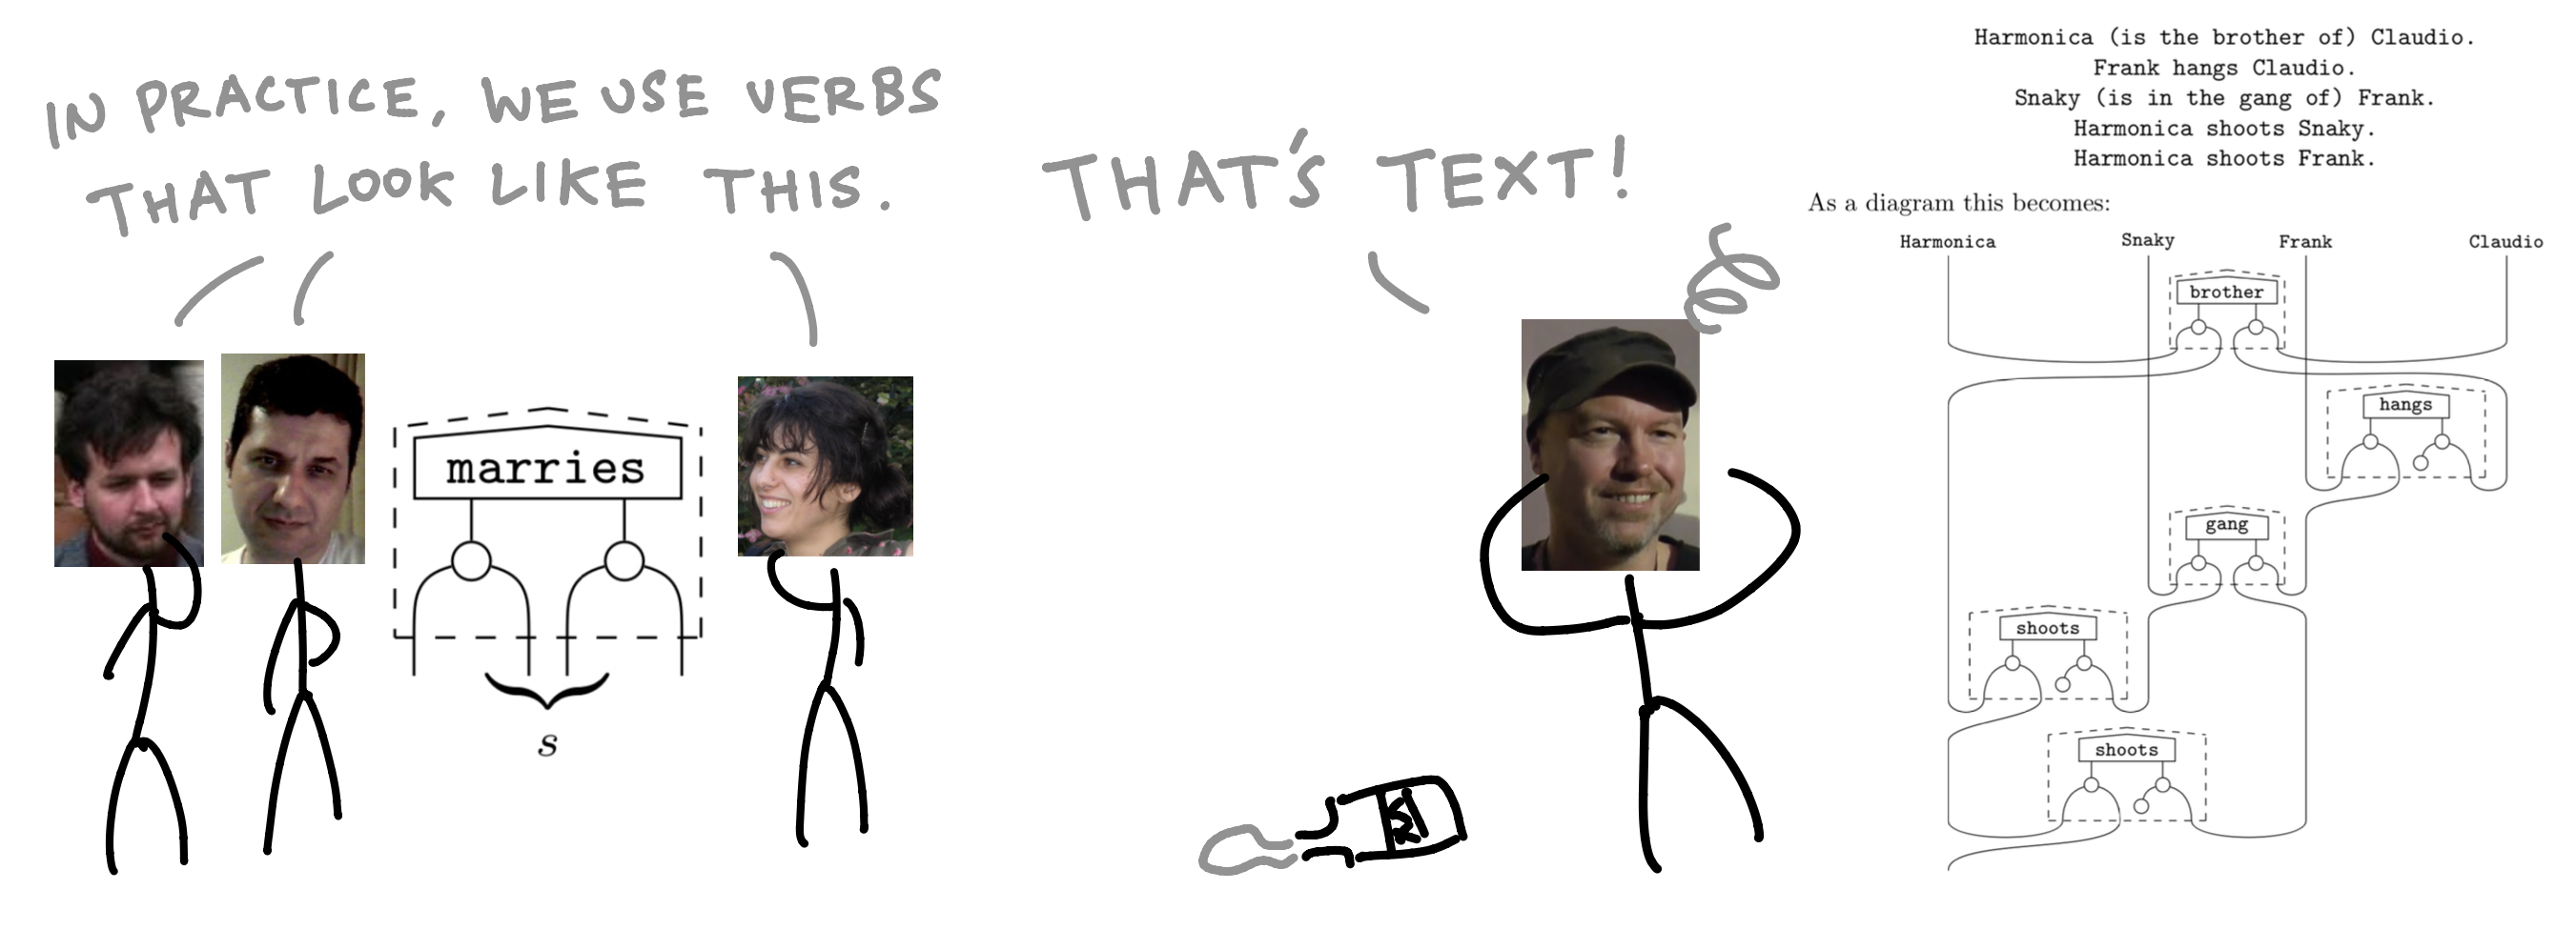
\includegraphics{figures/cartoons/discocirc1}}
\caption{It is a common evolutionary step in linguistics that theories `break the sentential barrier', moving from sentence-restricted to text- or discourse-level analysis \bR CITE \e. The same thing happened with DisCoCirc, due to a combination of practical constraints and theoretical ambition. On the practical side, wide tensors were (and remain) prohibitively expensive to simulate classically and actual quantum computers did not (and still do not) have many qubits, hence in practice pregroup diagrams were reduced to thinner and deeper circuits, often with the help of an additional simplifying assumption that sentence wires were pairs of noun wires in the illustrated form on the left. Theoretically, seeking dynamic epistemic logic, Bob had an epiphanous hangover (really) where he envisioned that these "Cartesian verbs" could be used in service of compositional text meanings, and he called this idea DisCoCirc \bR CITE \e.}
\end{figure}

\begin{figure}[h!]
\centering
\scalebox{1}{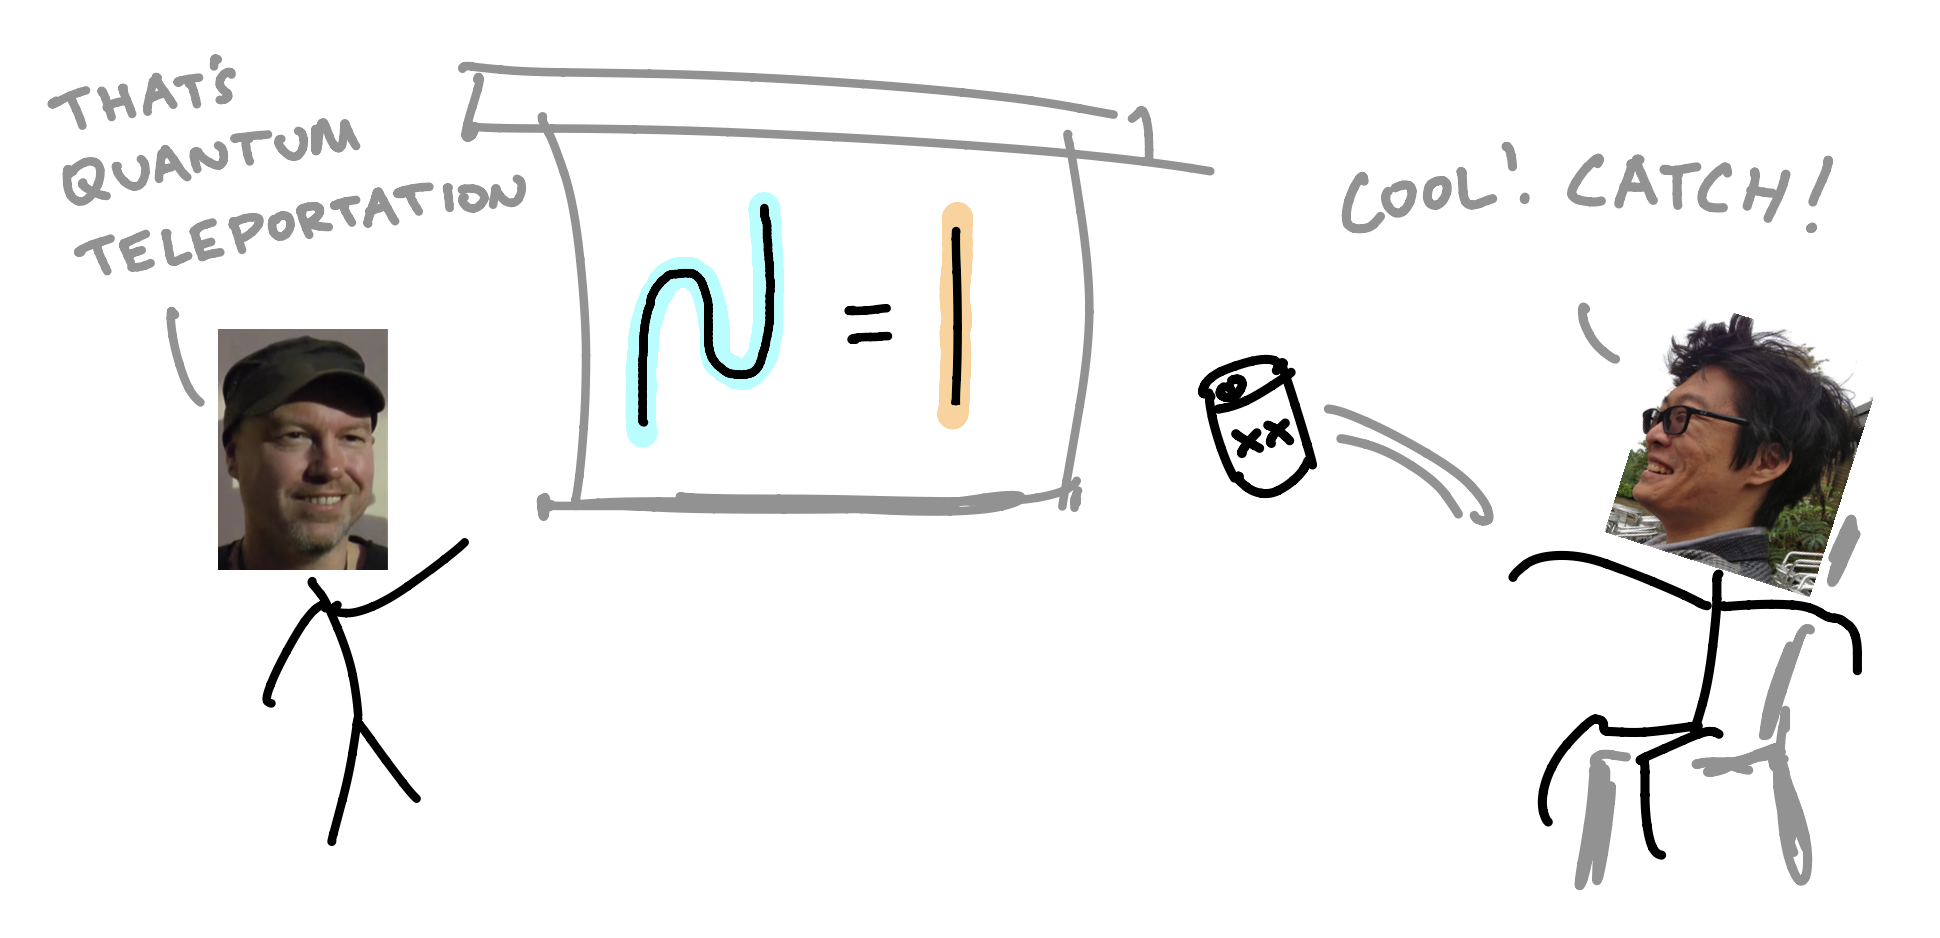
\includegraphics{figures/cartoons/v1}}
\caption{I met Bob in my master's in 2019, where he taught the picturing quantum processes course. When quantum teleportation was explained in half a minute by a diagram, I decided to pursue a DPhil in diagrammatic mathematics. In the last lecture, I threw Bob a cider, after which he seemed to like me. I did not know he was an alcoholic.}
\end{figure}
\clearpage

I was shanghaied into thinking about diagrams for language. I was deeply dissatisfied with the content from the standpoint my own intellectual integrity. Firstly, there seemed to me an unspoken claim that the presence of cups in pregroup diagrams (which implied a noncartesian and hence large tensor product) made it necessary to use quantum computers to effectively compute pregroup diagrams. I just could not believe that my brain required quantum computation to understand language. This implicit claim of kinship between quantum and linguistics was further entrenched by the analysis of the relative pronoun in terms of frobenius algebras, since spiders in $\mathbf{Vect}^\otimes$ were the \emph{sine qua non} of categorical quantum mechanics. The best steelman for spiders I have is that frobenius algebras (which are central to bicategories of relations \bR CITE \e) just happen to be a ubiquitous mathematical structure that are well-suited to express the mathematics of connections, both in language and in quantum.\\

Second, representing the content of a sentence as a vector in a sentence-vector-space did not sit well with me, since this move meant that the only meaningful thing one could do with two sentences was take their inner-product as a measure of similarity. Moreover, I had the theoretical concern that language is in principle indefinitely productive, so one could construct a sentence that marshalled indefinitely many nouns, and at some point for any finite vector space $s$ one would run out of room to encode relationships, or else they would be cramped together in a way that did not suit intuitions about the freedom of constructing meanings using language. I always believed in the existence of a simple, practical, and intuitive categorical, compositional, and distributional semantics; I just didn't believe that the role of quantum -- however helpful or interesting -- was \emph{necessary}.

My first unsatisfactory attempt was in my Master's thesis \bR CITE \e. It had been known for a while that a free autonomous category construction by Delpeuch \bR CITE \e could potentially eliminate some of the cups in pregroup diagrams, yielding what amounted to a method to transform a pregroup diagram into a monoidal string diagram in the shape of a context-free grammar tree. This trick had the limitation that freely adding directed cups and caps to a string diagrammatic signature did not turn a symmetric monoidal category into a (weakly) compact closed one, rather just into a monoidal category where the original wires had braidings, but all the new left and right dual wires did not; this presented difficulties in accounting for iterated duals for higher-order modifiers such as adverbs in grammatical types, and had nothing to say about spiders. I tried to generalise this trick to `freely' adding arbitrary diagrammatic gadgets to string diagrams, but my assessor Samson pointed out that it was nontrivial to determine whether such constructions were faithful. In retrospect the free autonomous completion of a parameterised \bR CITE \e markov category \bR CITE \e is in the ballpark of dequantumfying pregroup diagrams, but I didn't learn about them until later, and that still wouldn't have addressed the issues that come with only having a sentence-wire.

\begin{figure}[h!]
\centering
\scalebox{1}{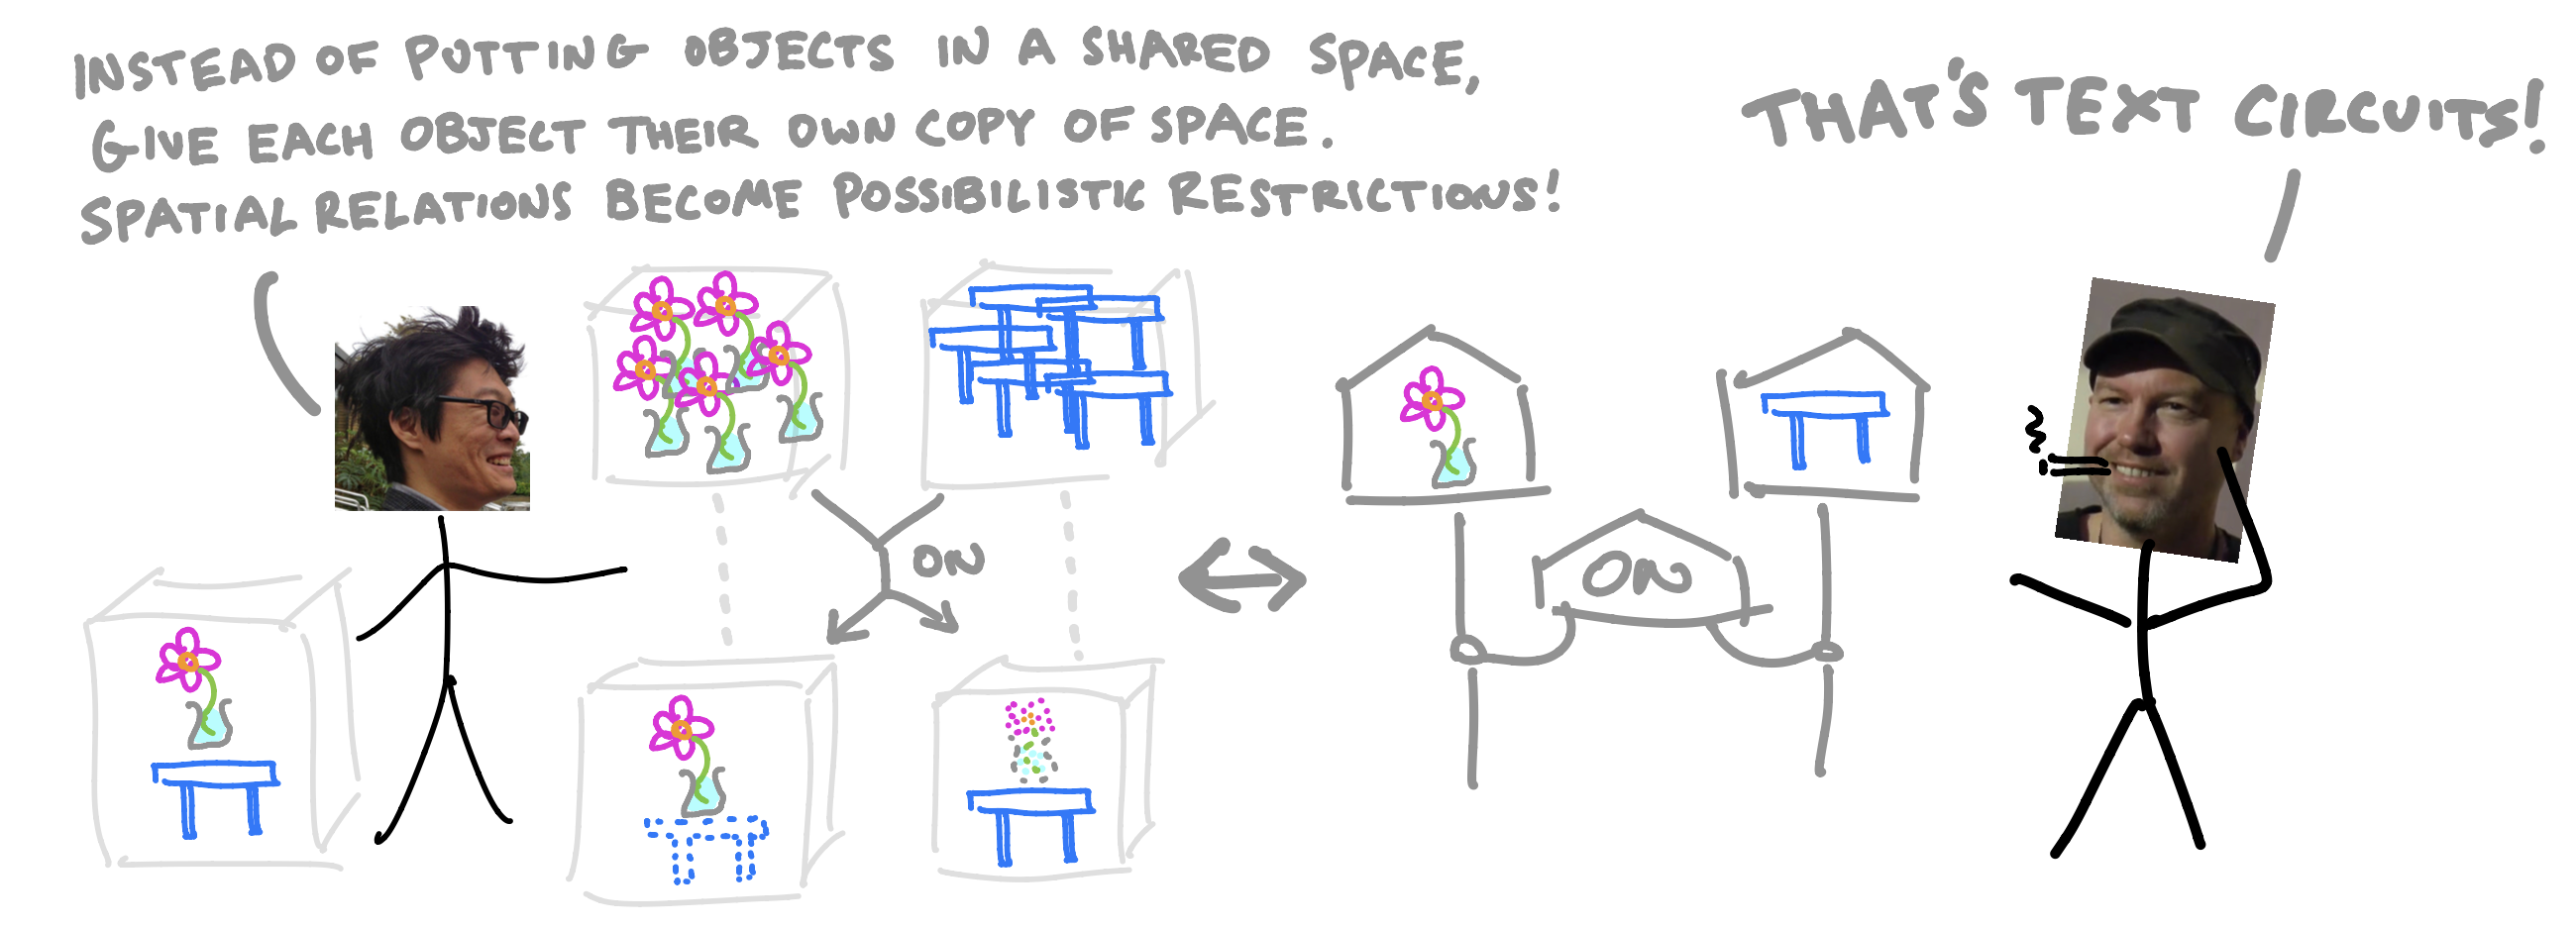
\includegraphics{figures/cartoons/circify1}}
\caption{Then COVID happened. During the first lockdown, I visited Bob's garden under technically legal circumstances, and I suggested a solution to the longstanding problem of representing linguistic spatial relationships. My theoretical concern was the culprit: the initial attempts at the problem failed because the approach was to find a single sentence object $s$ in which one could paste the data of arbitrarily many distinct spatial entities. The simple solution was a change in perspective.}
\end{figure}

\begin{figure}[h!]
\centering
\scalebox{1}{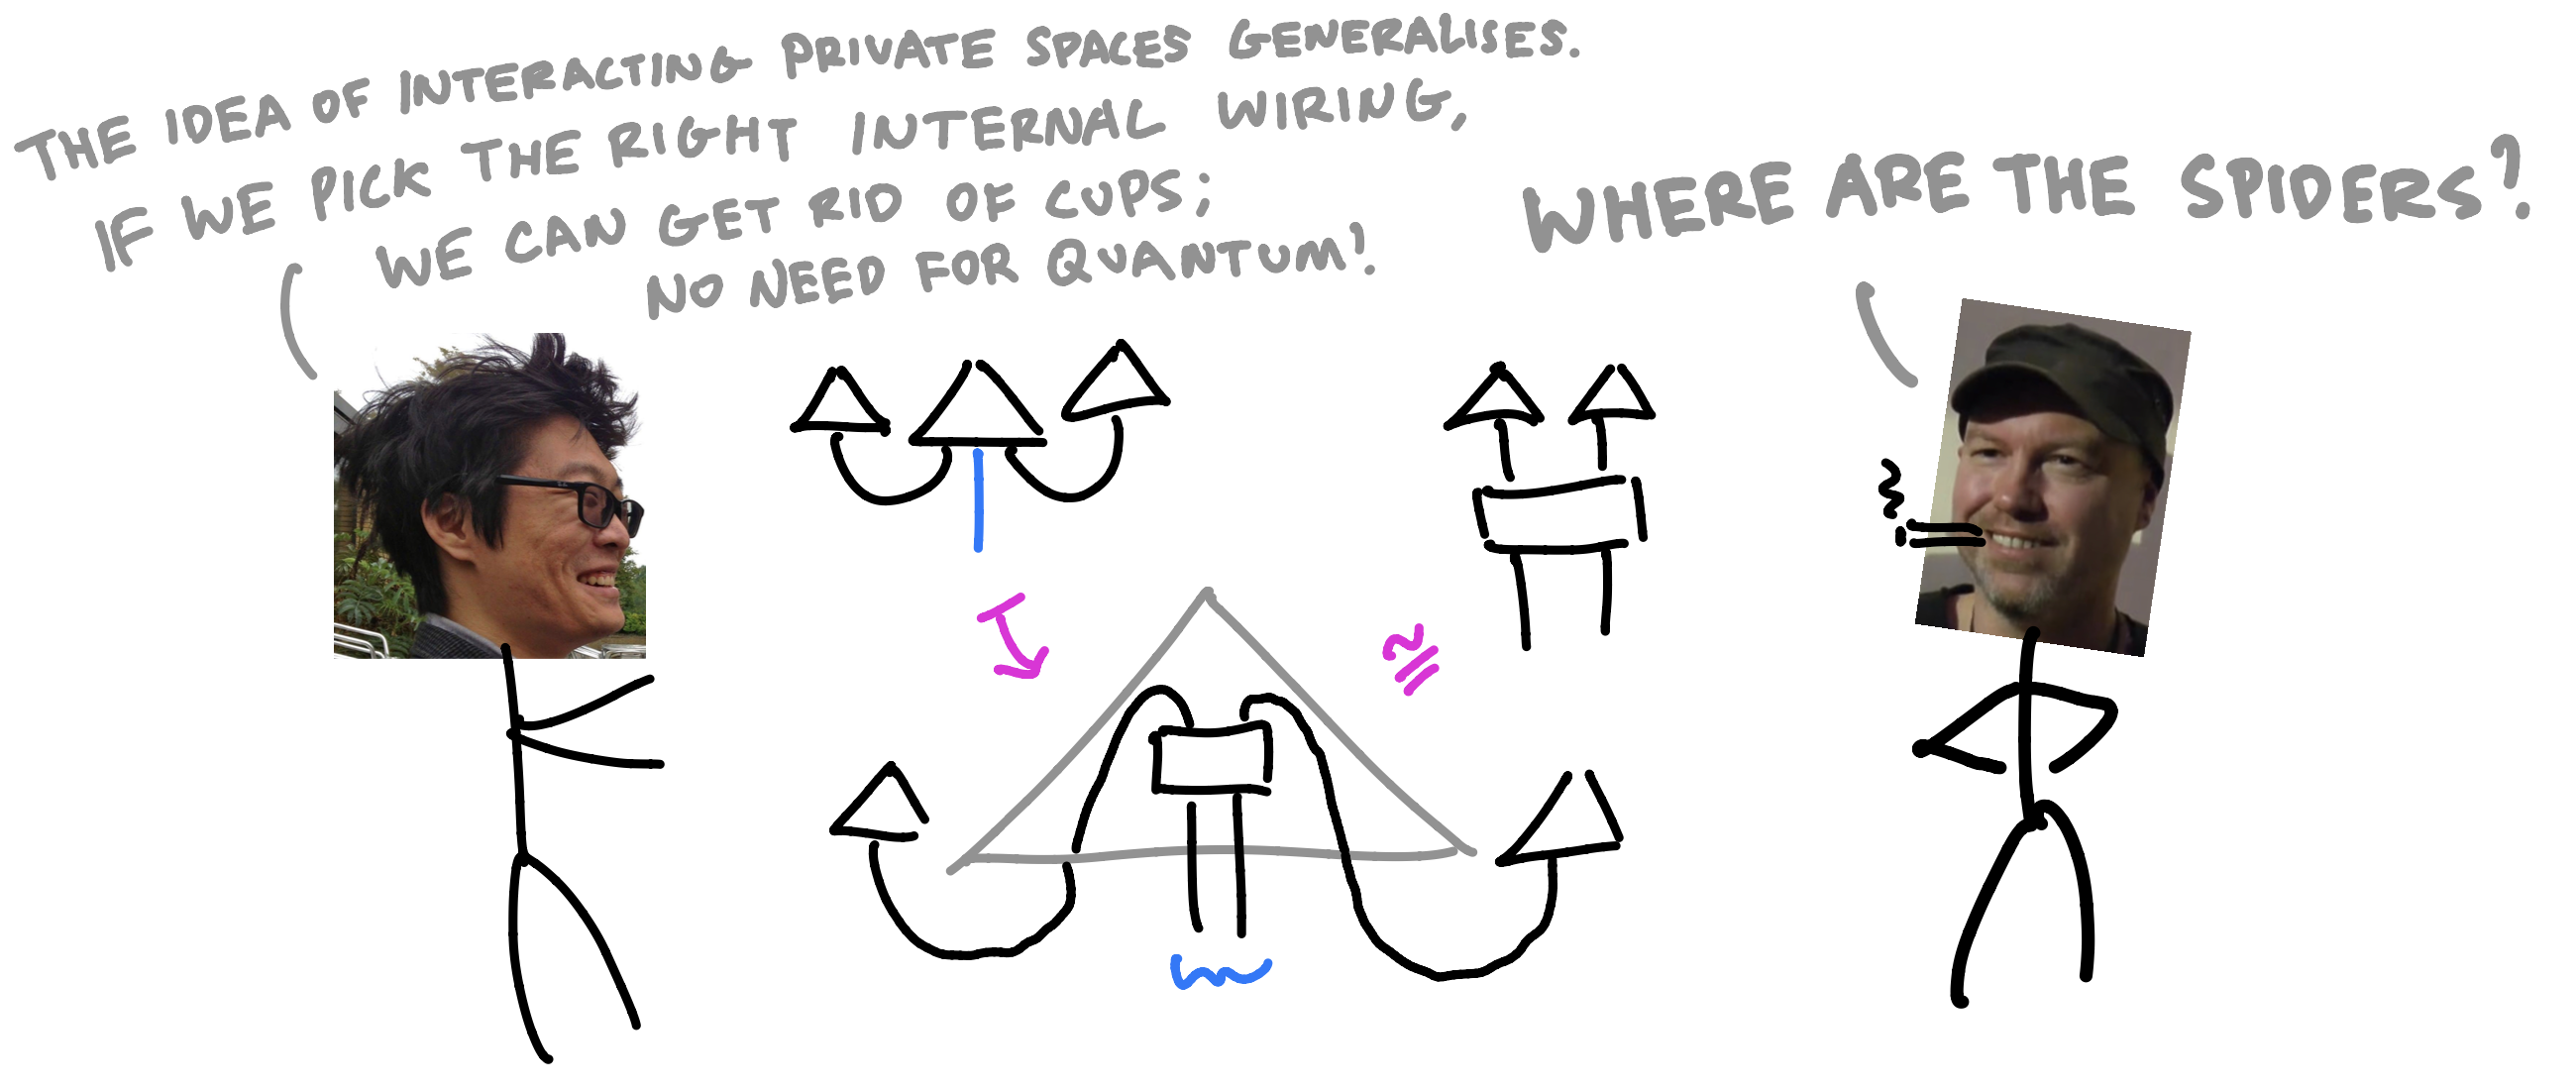
\includegraphics{figures/cartoons/circify2}}
\caption{That this move of splitting up the sentence-wire into a sentence-dependent collection of wires was sufficient to solve what had appeared to be a difficult problem prompted some re-examination of foundations. The free autonomisation trick in conjunction with sentence-wire-as-tensored-nouns seemed promising, but it became clear that right way to drown a DisCoCat thoroughly was to explain and eliminate the spiders.}
\end{figure}

\begin{figure}[h!]
\centering
\scalebox{1}{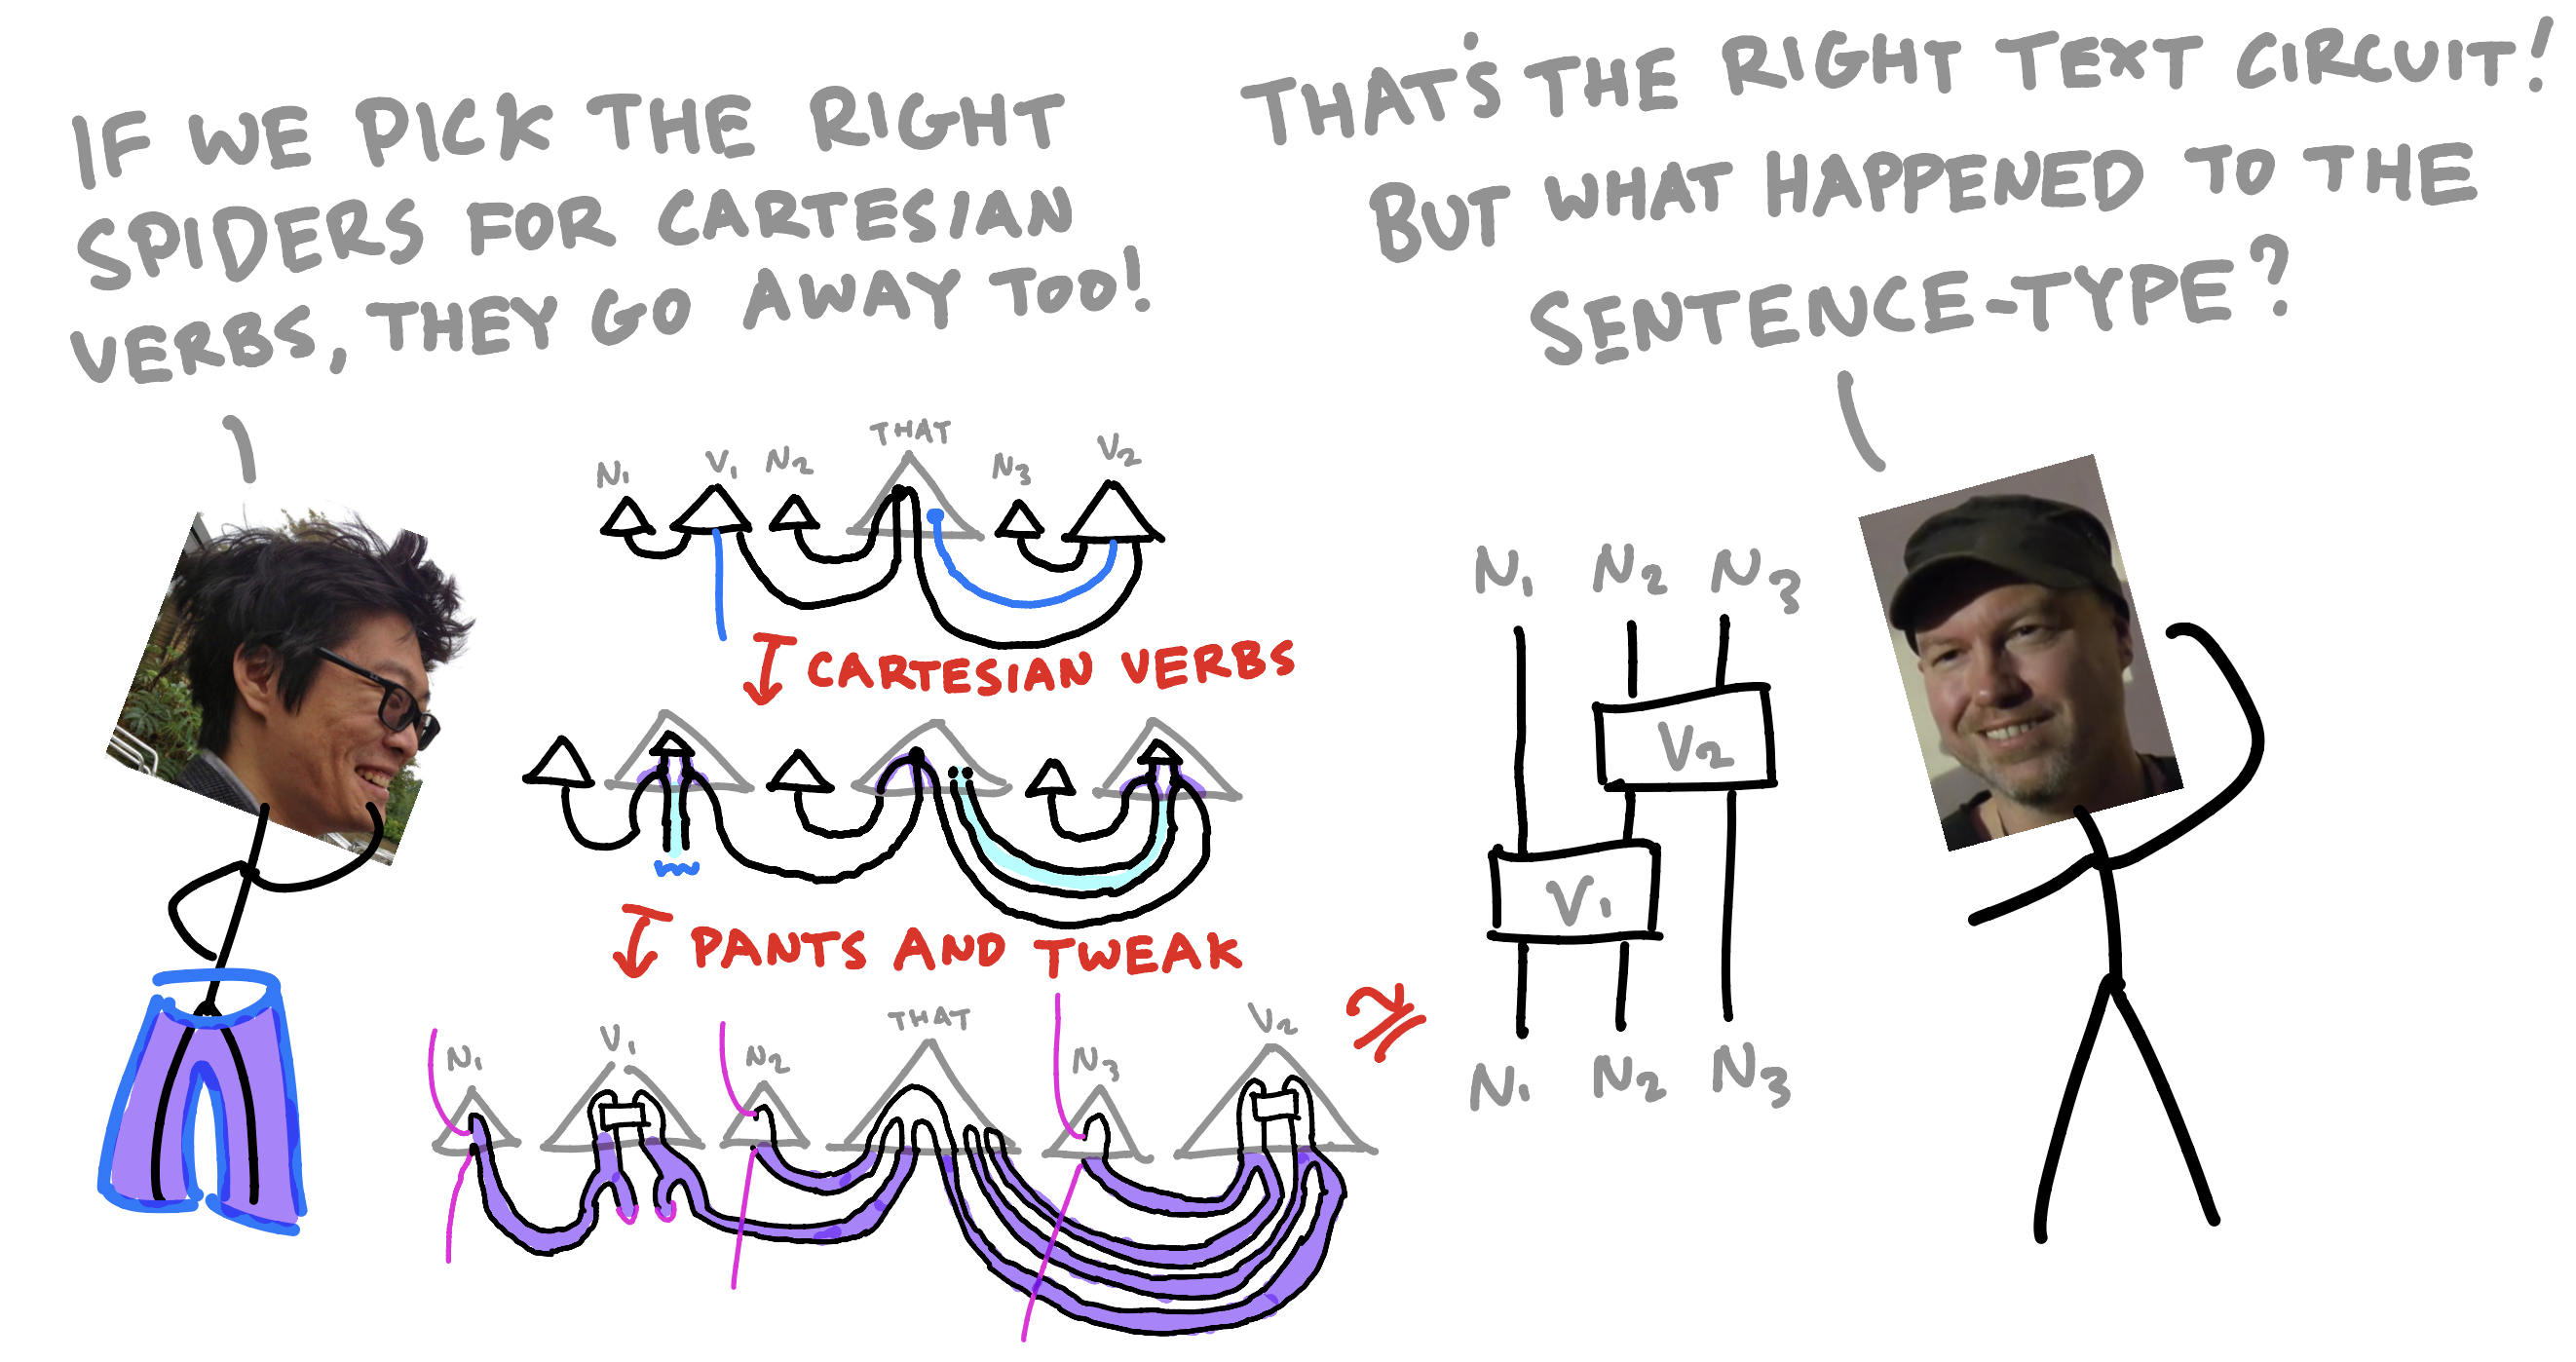
\includegraphics{figures/cartoons/circify3}}
\caption{I then discovered that by interpreting spiders as the well-known "pair of pants" algebra in a compact closed monoidal setting allowed for a procedure in which the final form was purely symmetric monoidal -- the absence of cups and caps meant that there was no practical necessity to interpret diagrams on quantum computers: \emph{any} computer would suffice. The role of spiders for relative pronouns was illuminated in the presence of splitting the sentence wire: the pair-of-pants are the algebra of morphism composition, and splitting the sentence wire into a collection of nouns allowed relative-pronoun-spiders to pick out the participating nouns to compose relationships onto.}
\end{figure}

\begin{figure}[h!]
\centering
\scalebox{1}{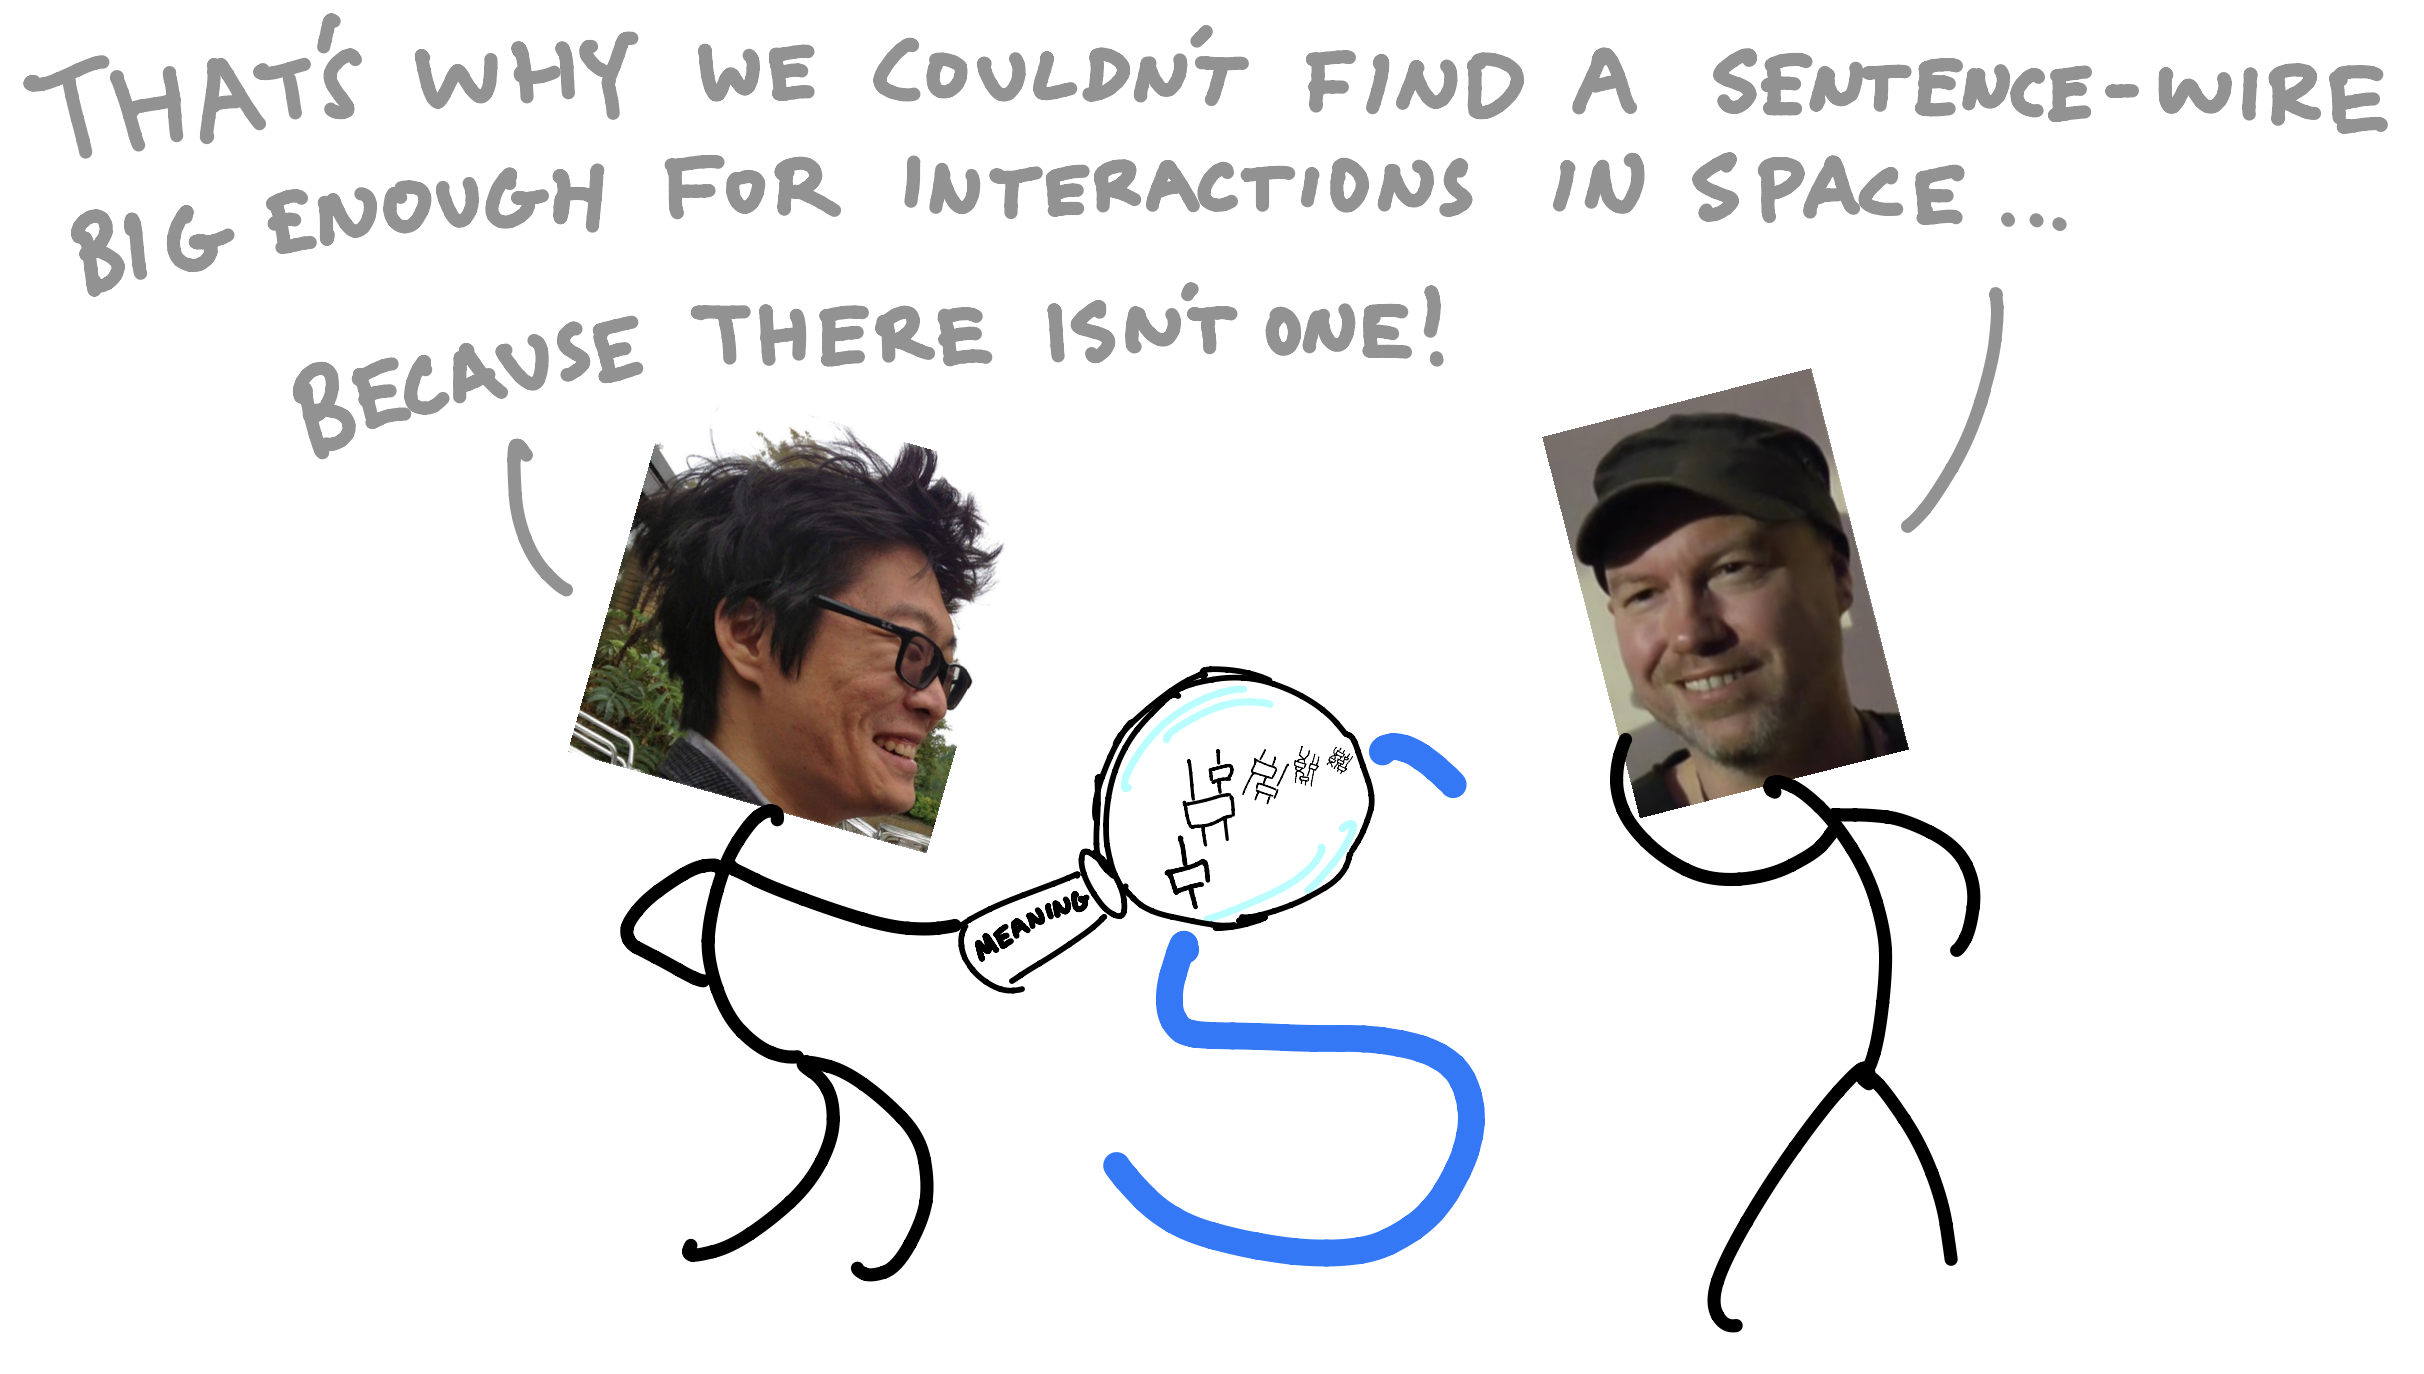
\includegraphics{figures/cartoons/nosent}}
\caption{A coherent conservative generalisation of DisCoCat with less baggage had emerged, or rather, DisCoCirc was placed to formally subsume DisCoCat. It was now understood that the sentence type was a formal syntactic ansatz for the sake of grammar, which was to be interpreted in the semantic domain not as a single wire, but as a sentence-dependent collection of wires. It was further realised that the complexity of pregroup diagrams was due to grammar -- the topological deformation of semantic connections to fit the one-dimensional line of language -- whereas the essential connective content of language could be expressed in a simple form that distilled away the bureaucracy of syntax.}
\end{figure}

\begin{figure}[h!]
\centering
\scalebox{1}{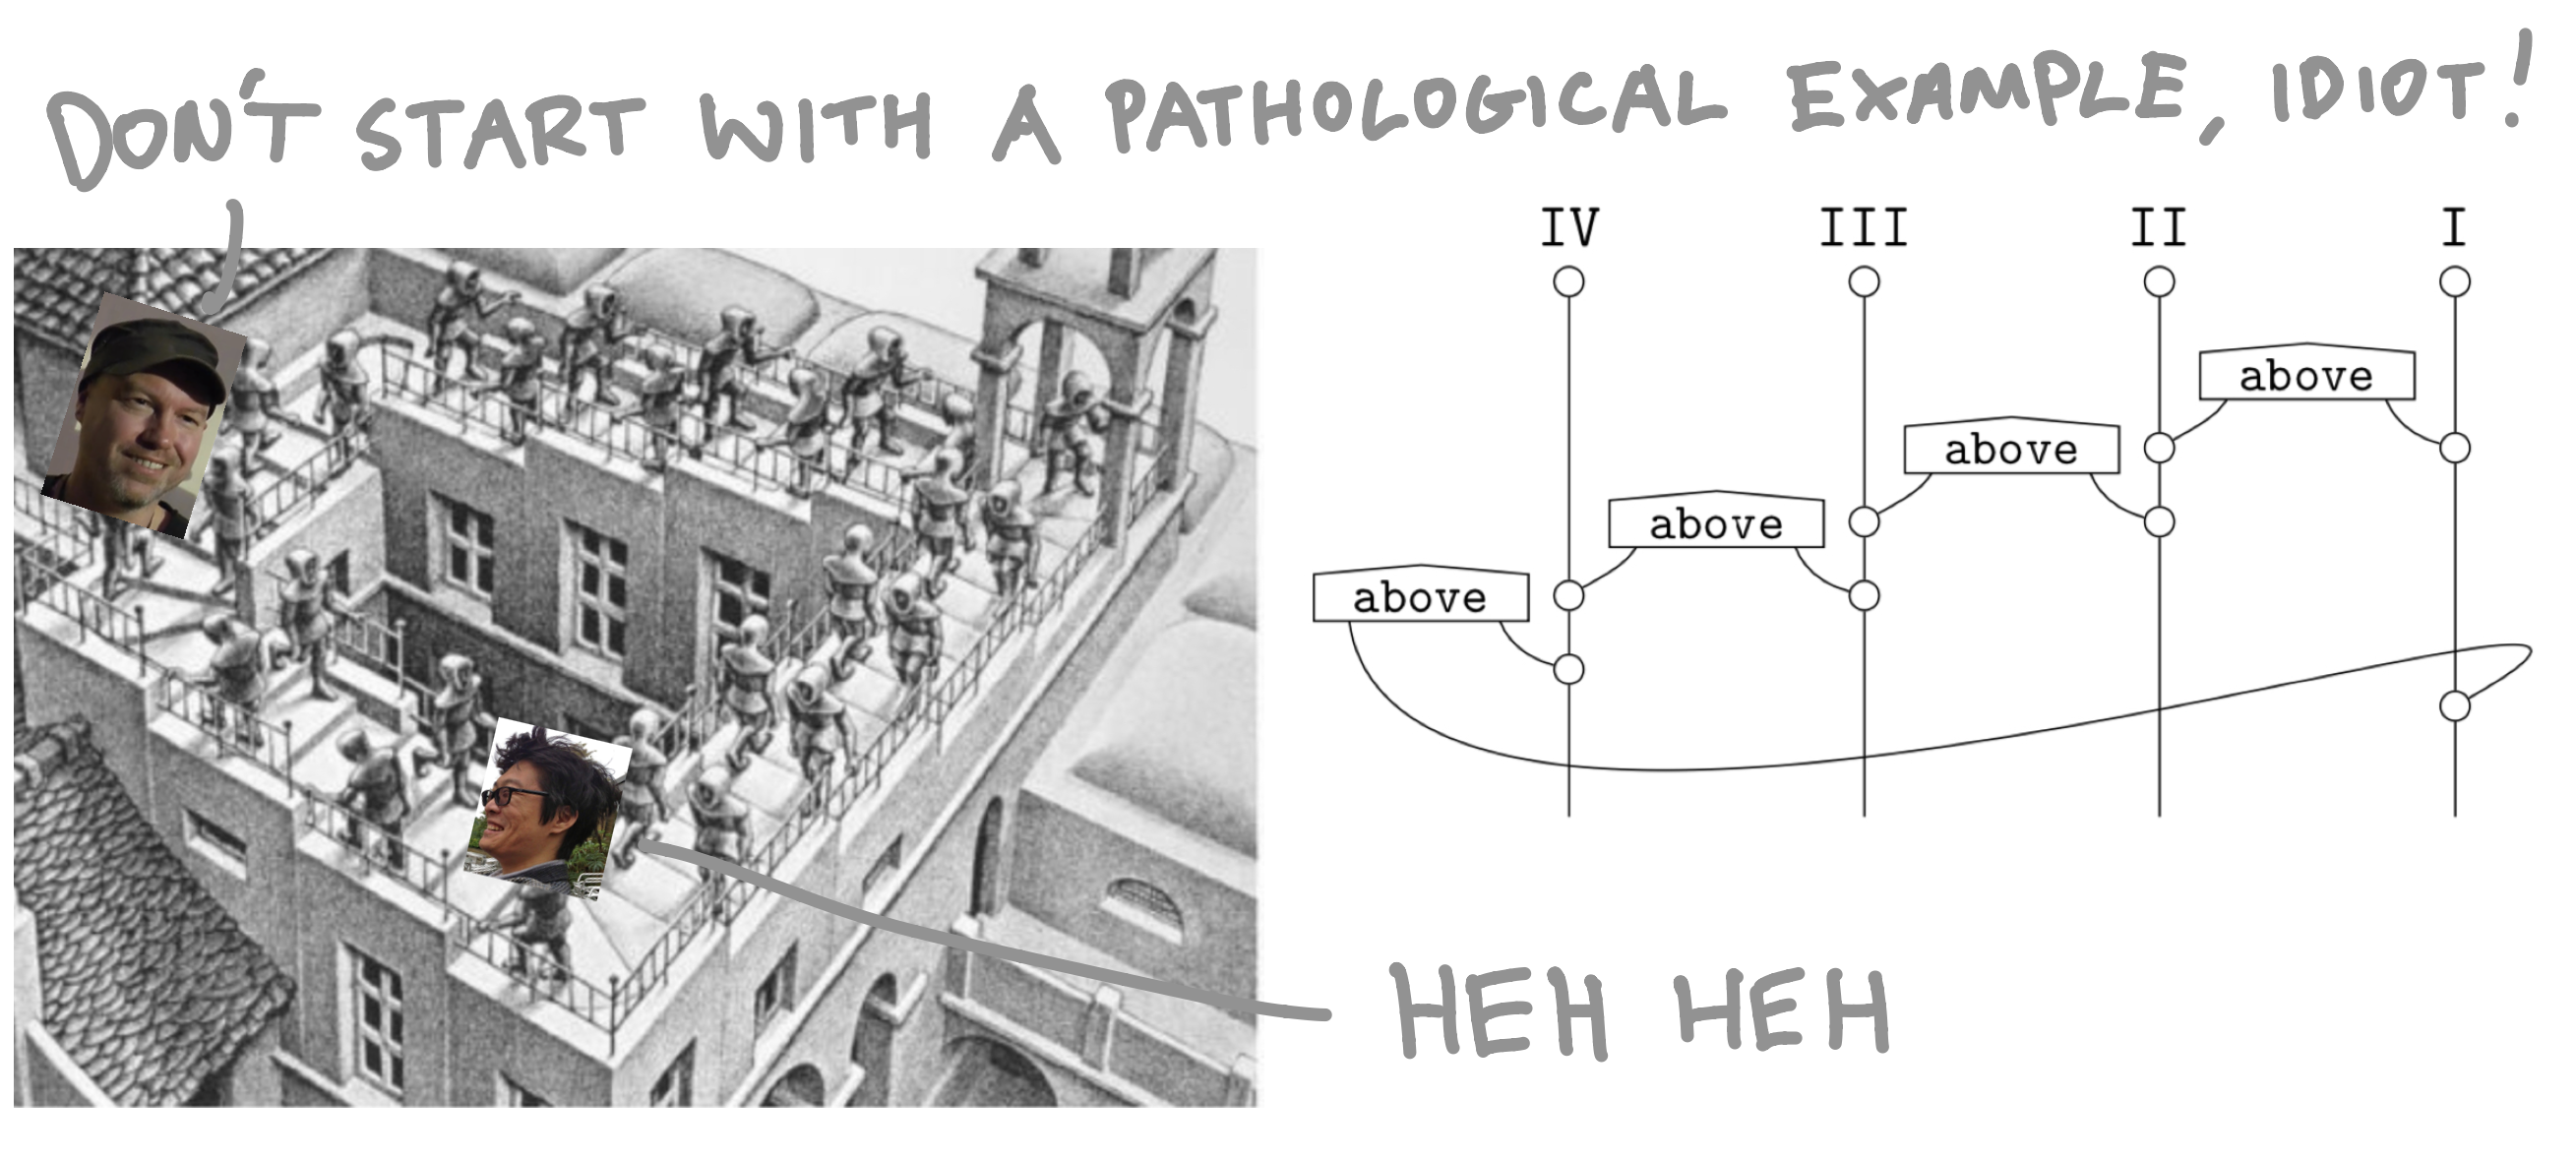
\includegraphics{figures/cartoons/space1}}
\caption{We wrote up the story about spaces in \bR CITE \e, the spiritual successor to \emph{interacting conceptual spaces I}. We could formally calculate the meanings of sentences that used linguistic spatial relations, all using a simple and tactile diagrammatic calculus.}
\end{figure}

\begin{figure}[h!]
\centering
\scalebox{1}{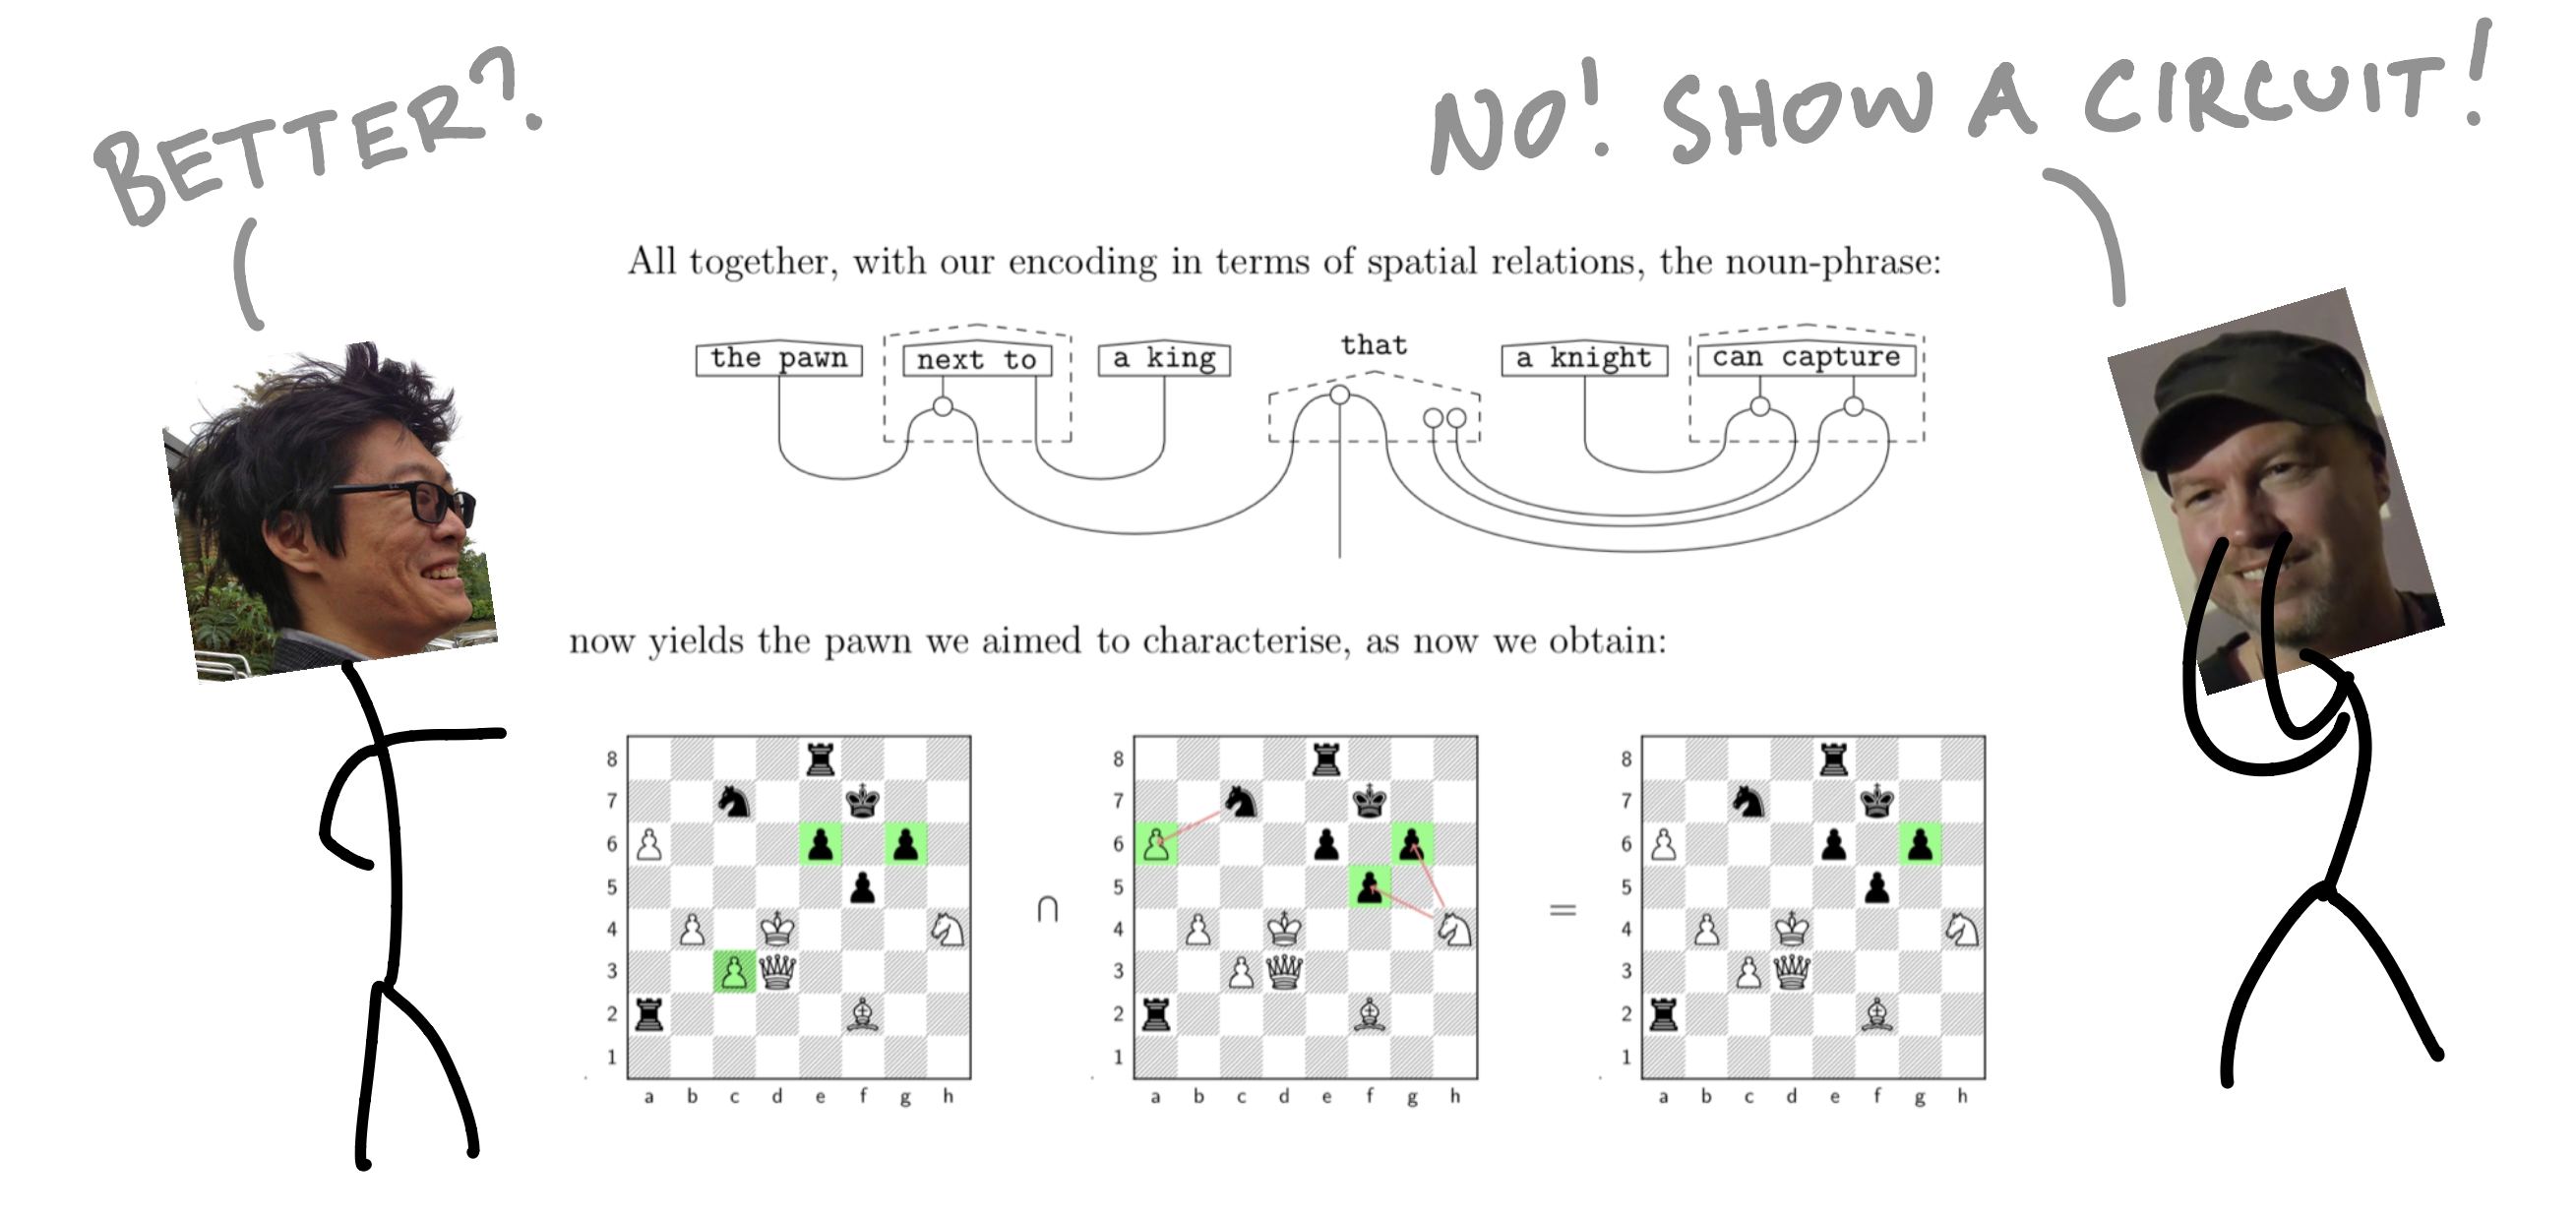
\includegraphics{figures/cartoons/space2}}
\end{figure}

\begin{figure}[h!]
\centering
\scalebox{1}{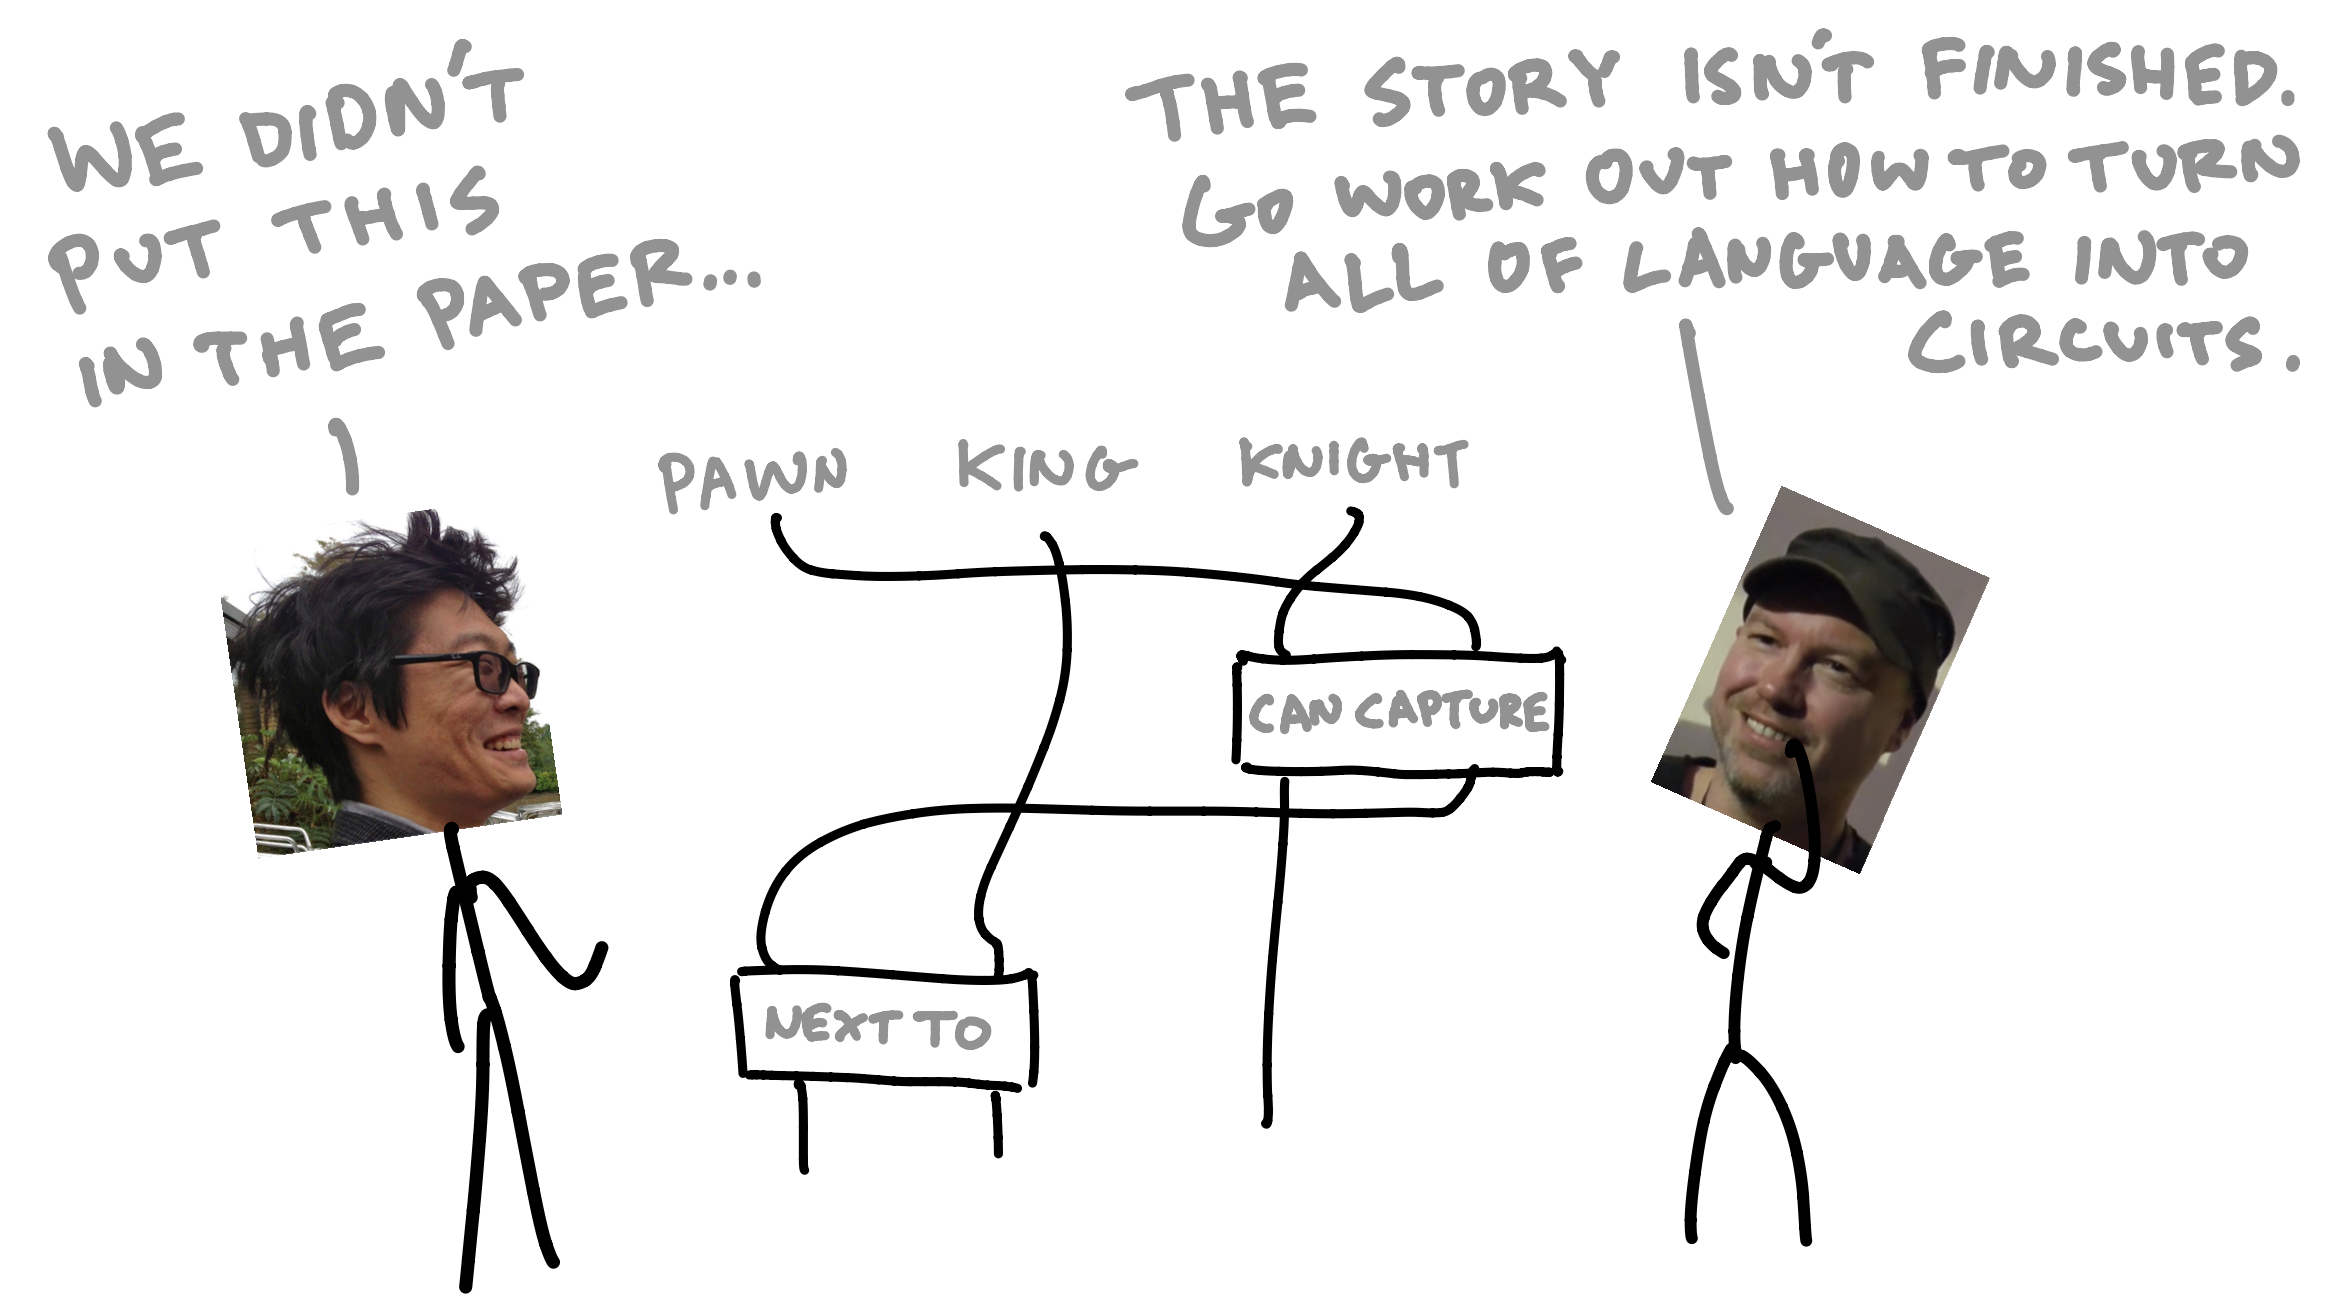
\includegraphics{figures/cartoons/space3}}
\caption{The paper on spatial relations actually came very late, because I was busy with Bob's ludicrous request to go turn "all of language" into circuits. I bitched and moaned about how I wasn't a linguist and how it was an impossible task, but I was in too deep to back out.}
\end{figure}

\begin{figure}[h!]
\centering
\scalebox{1}{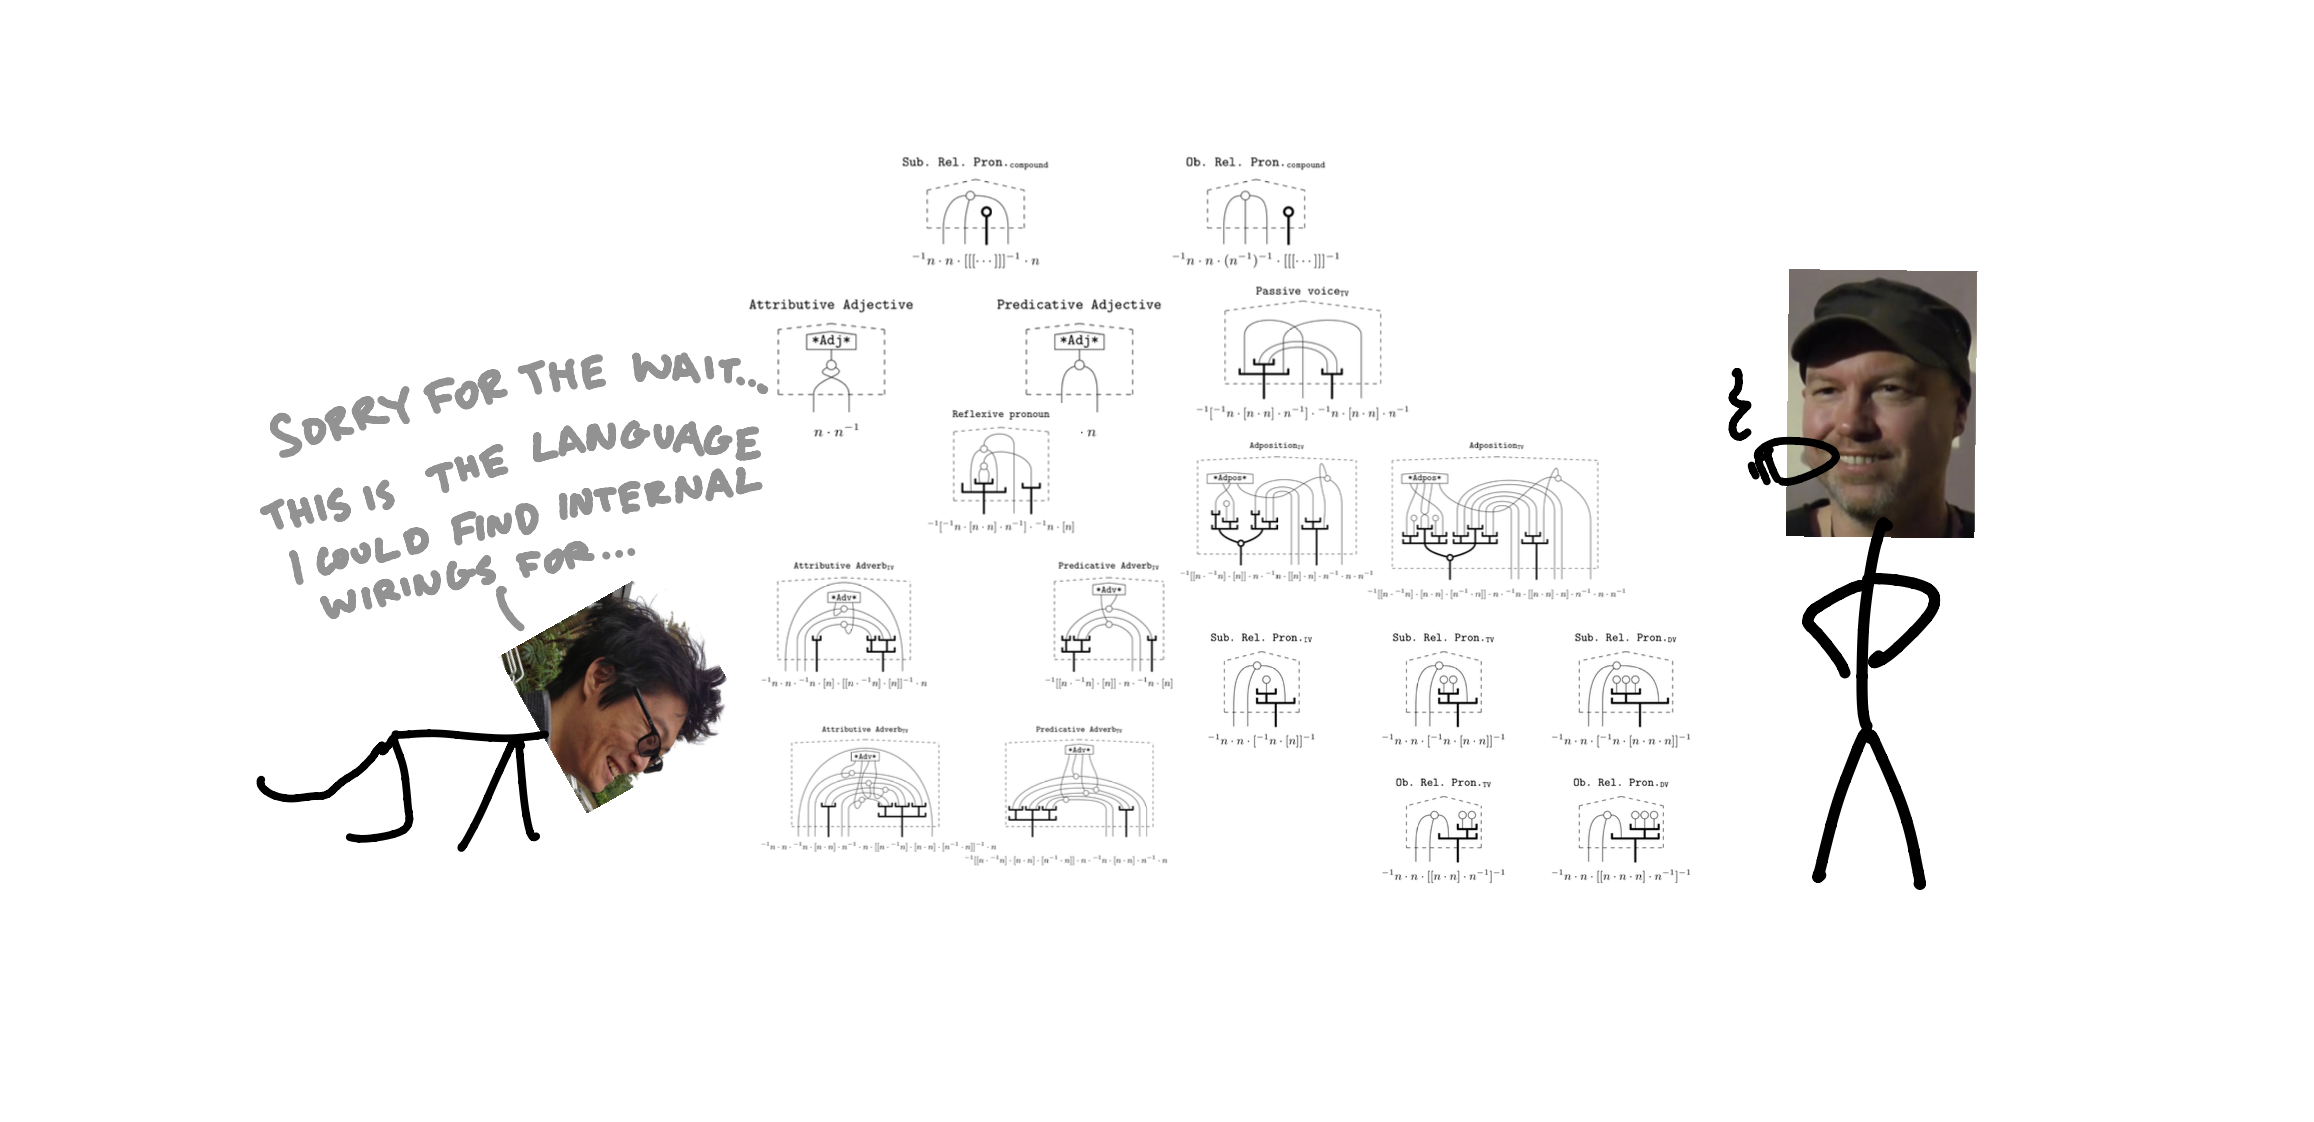
\includegraphics{figures/cartoons/pregroup1}}
\caption{I suppose the nice thing about aiming for the moon is that even failure might mean you leave orbit. So I settled for what I thought was a sensible fragment of English, for which I devised internal wirings and an algorithm that transformed pregroup diagrams with the internal wirings into circuit form. Many tiring diagrams later, I presented my results in the first draft of "distilling text into circuits".}
\end{figure}

\begin{figure}[h!]
\centering
\scalebox{1}{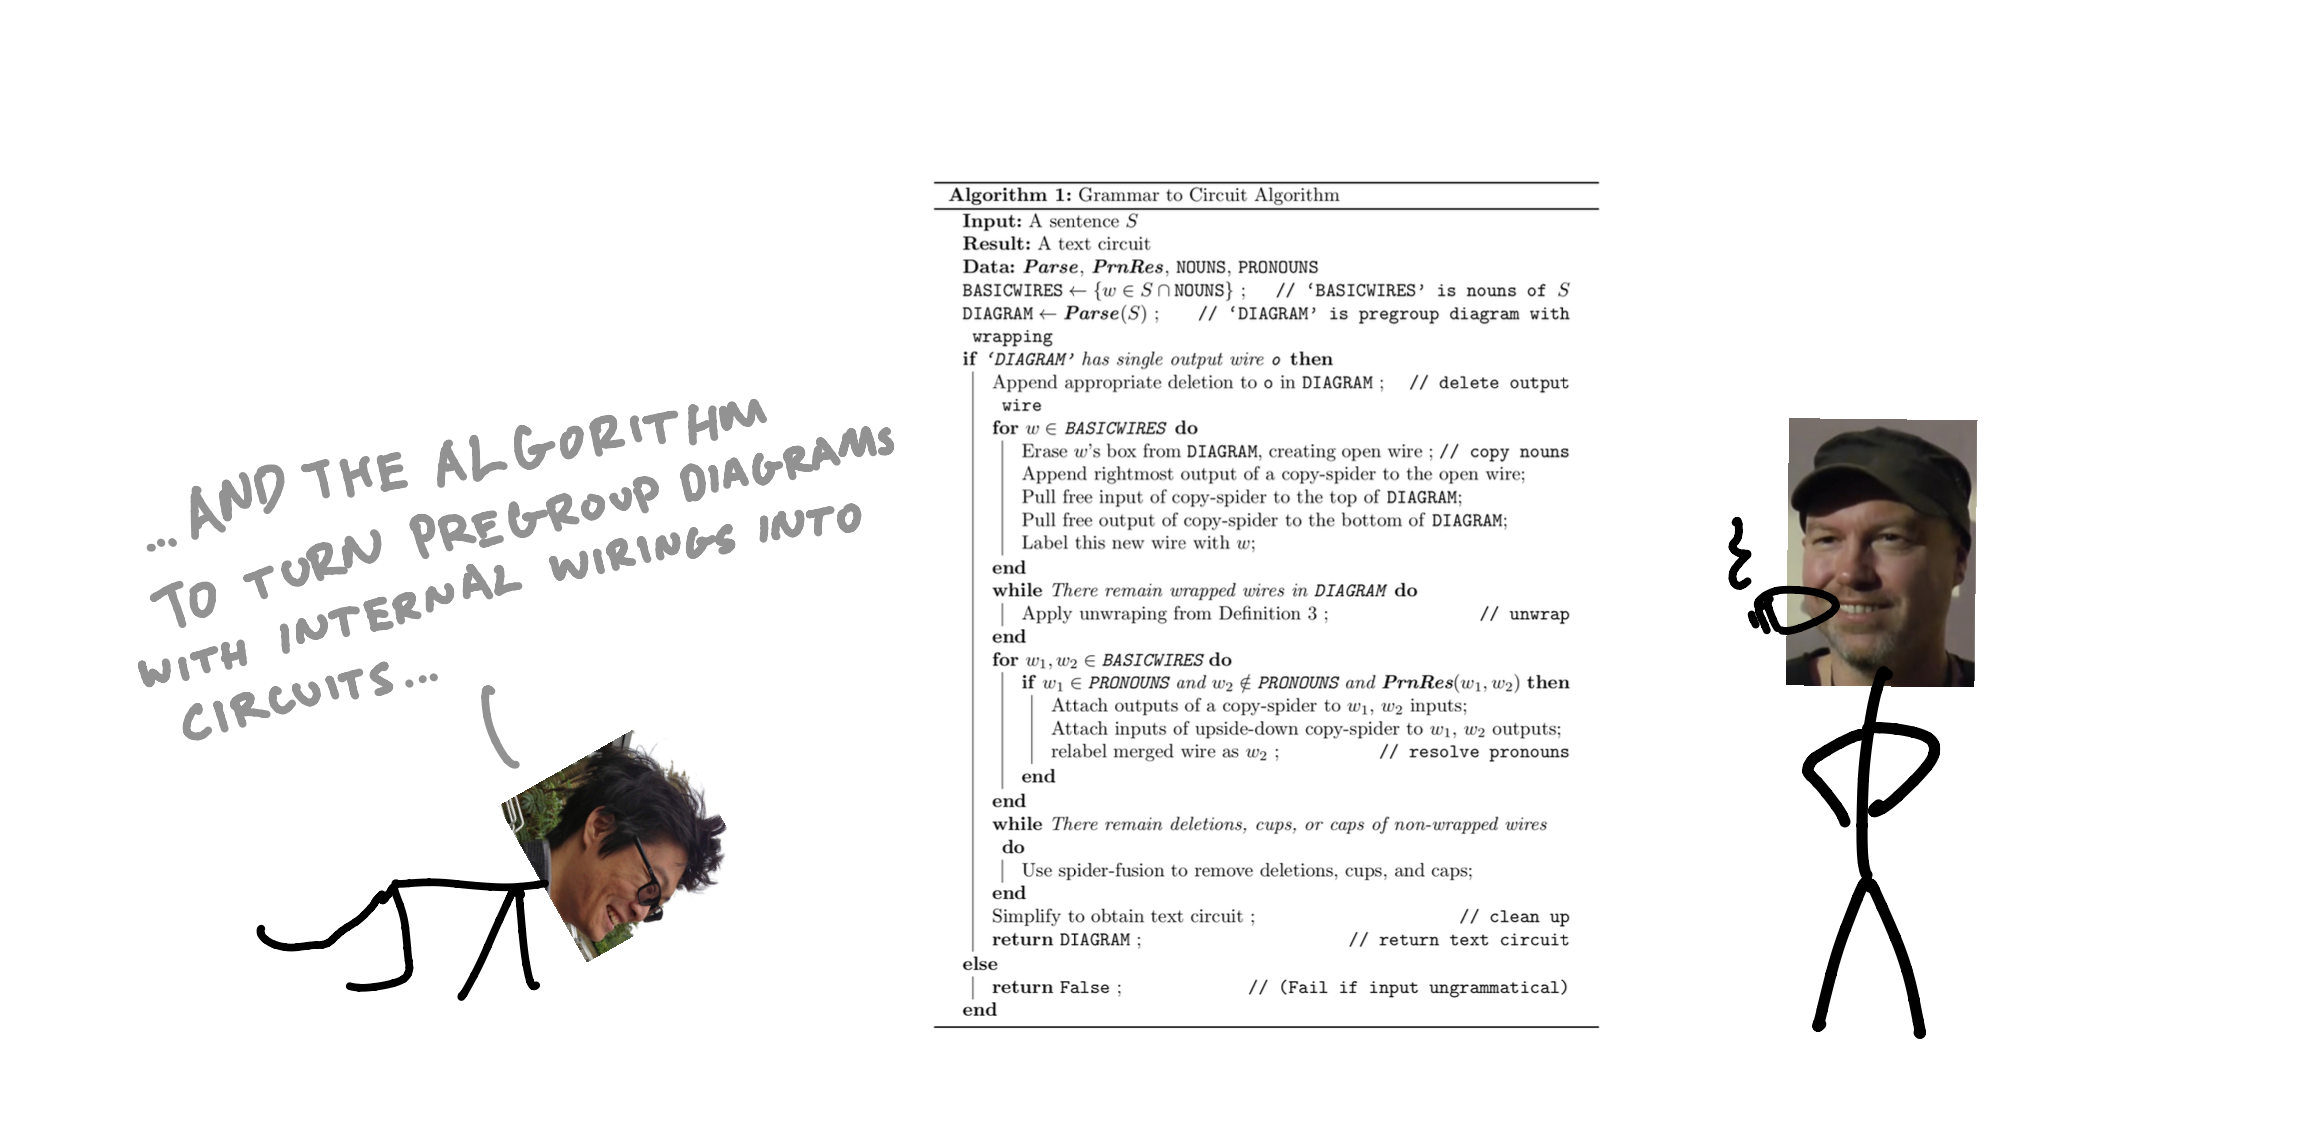
\includegraphics{figures/cartoons/pregroup2}}
\end{figure}

\begin{figure}[h!]
\centering
\scalebox{1}{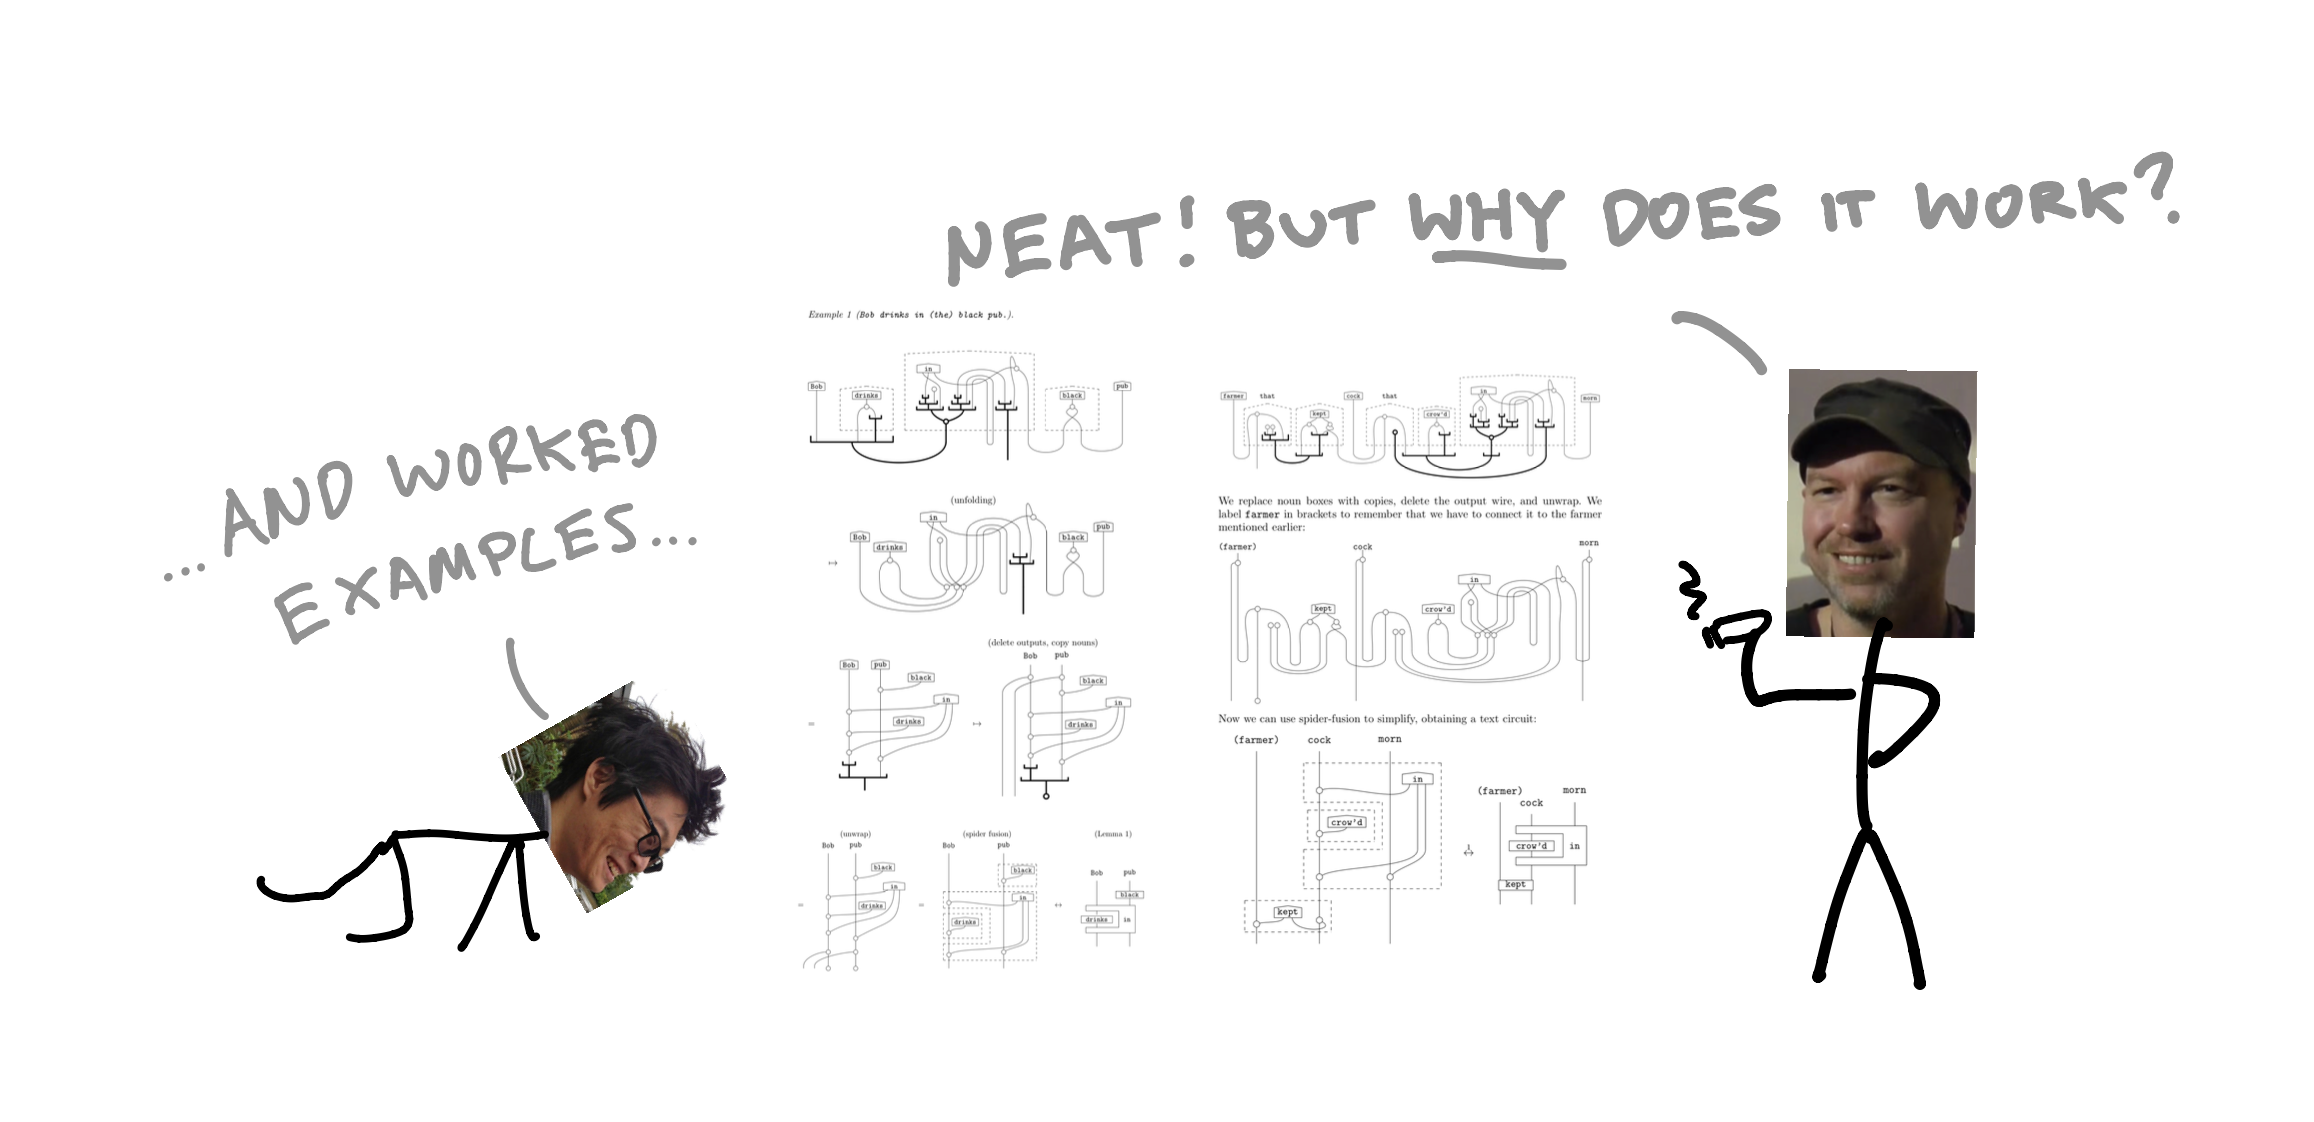
\includegraphics{figures/cartoons/pregroup3}}
\end{figure}

\begin{figure}[h!]
\centering
\scalebox{1}{
\includegraphics{figures/cartoons/pregroup4}}
\caption{Bob had a good point. Everything worked, but we had no understanding as to why, and accordingly, whether or not it would all break. At this point in time, Jonathon Liu, a masters' student I tutored during COVID, had committed the grave error of thinking diagrams were cool, and was now hanging out with me and Bob. After understanding the procedure, Jono independently devised the same arcane internal wirings as I had, but neither of us could explain how we did it. So we had evidence of an underlying governing structure that was coherent but inarticulable.}
\end{figure}

\begin{figure}[h!]
\centering
\scalebox{1}{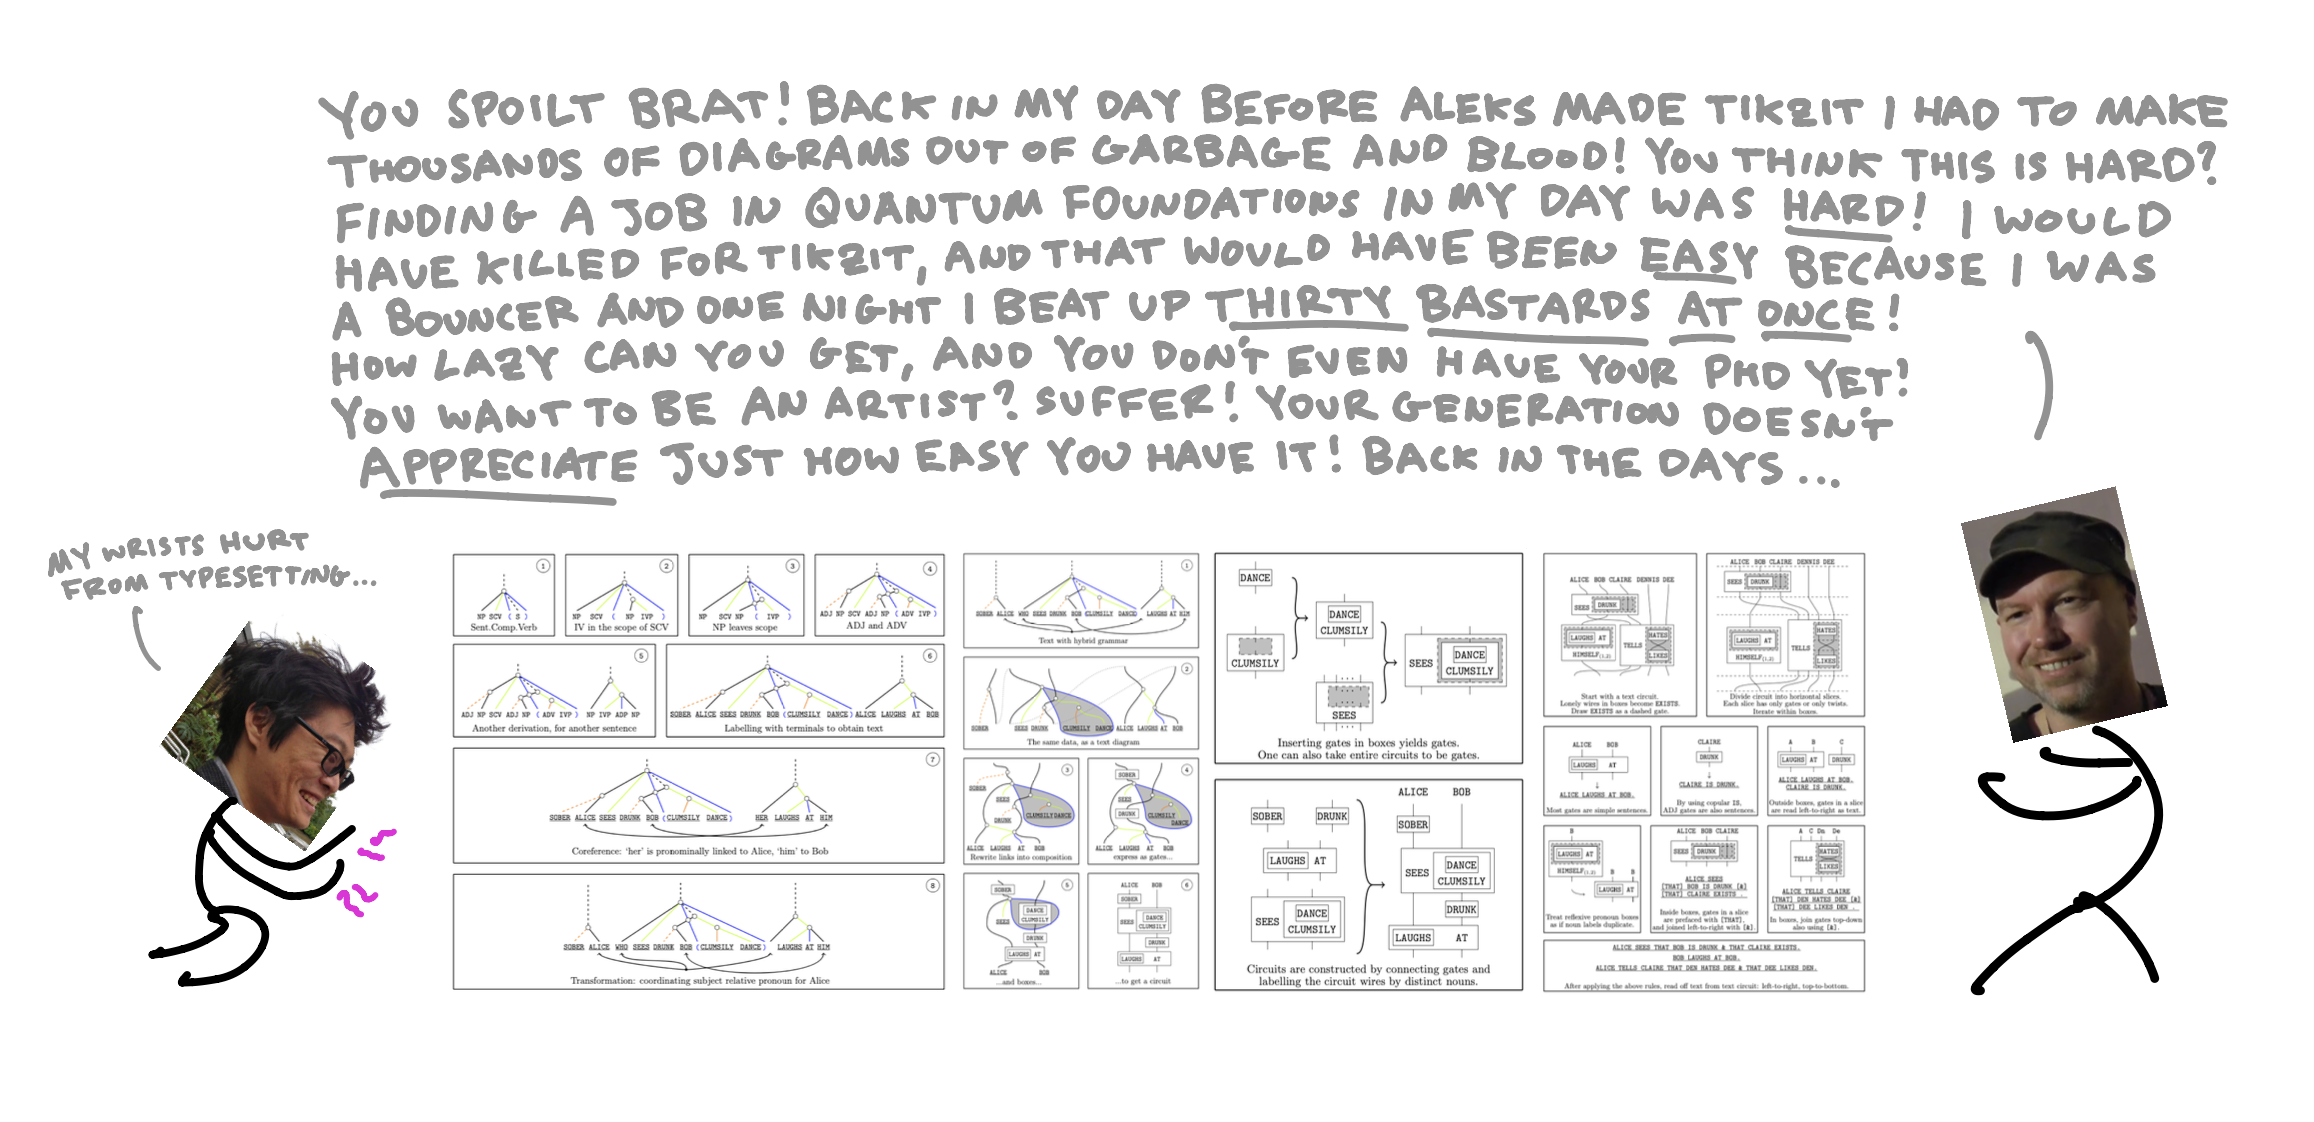
\includegraphics{figures/cartoons/bigpaper1}}
\caption{I realised that our intuitions were coming from an implicit productive grammar, rather than a parsing one, and that the path of least resistance for obtaining formal guarantees for the language-to-circuit procedure was to just handcraft a generative grammar for the fragment of language we were interested in. This meant scrapping everything in the first draft and starting again from scratch. Bob always had a word of gentle encouragement, giving me the motivation to persevere.\\

So now we had two ways to obtain text circuits. One from pregroups (which Jono had extended the technique for to CCGs in his master's thesis \bR CITE \e), and one from handcrafted productive grammars. Then came time for me to write my thesis, and there were three salient questions I wanted to address.\\
Firstly, what are internal wirings?\\
Secondly, how do text circuits relate to other generative grammars?\\
Thirdly, what are text circuits good for?\\
These questions are now what the rest of the thesis seeks to answer.
}
\end{figure}\label{sec:previously}
\additionalchapter{\chapfrac{1}{2}}{Corrections}\label{ch:oneandhalf}
\chapter{Corrections, as a letter to the reader}

Dear Reader,

How are you? I am well, thank you.

Forgive me for writing in this informal register; it is easier for me than the academic style (which I am no good at), and I would like to get these corrections done as painlessly as possible. You see, in the year or so it has taken for me to get around to these corrections, a lot has happened. I have gotten married, and I am soon to be a father. So I've learnt that there are more important things in life than a thesis, and I have otherwise been busy. While we are on apologies, please forgive me also for the tone of this work, which vacillates between serious and light; in my defense, I am constitutionally a trifler \cite{} (or else I wouldn't have gotten into formal linguistics), and I am still in the process of finding my voice as a writer.

There are several things I would like to get through in this letter, the main purpose of which is to settle most of the substantive corrections (recommended to me by my examiners Stefano Gogioso and Jules Hedges) in one go. I should preface by reminding you that all of this is written with a bit of distance from the rest of the work, and also that any opinions expressed here are strictly my own.

\section{Does it work?}

In the most important sense, no.

I will elaborate what I mean. There is a classical conception of structured approaches to AI/ML that permits capacities that go beyond what connectionist approaches are capable of, grounded in a kind of quasi-magical conception of mathematics as the ultimate form of understanding of --- and hence control over --- a phenomenon. It appears that part of the intellectual shock of generative AI is that one does not need to understand the mechanics of complicated phenomena in order to reliably induce them, given sufficient data and compute. This is obviously disappointing to many, and the highest sort of achievement that this thesis could have achieved is to have been a source of hope. Even a year ago the prospects seemed grim, and part of what took me so long to write the introduction was to compromise the positive vision from some demonstration of the complete superiority of structured approaches (basically no longer tenable after the advent of ChatGPT with RLHF) to something weaker, such as a performant way to synthesise structural/symbolic and connectionist approaches that has some other kind of benefit, such as "interpretability" (whatever that means.)

So taking \emph{"does it work?"} to mean \emph{"does it justify the activity of mathematically formulating the structure of language with respect to non-instrinsic measures of value (such as practical application)?"}, the answer is no, modulo most measures of value that people would care about. I say this because we've done some experiments.

\subsection{Have experiments been done?}

The approaches sketched out in Section \ref{} have been tried with neural networks in various ways by masters' students taking the Distributed Models of Meaning course offered in MFoCS here at Oxford, and separately it has been tried in the quantum setting \ref{} by talented scientists and engineers at the company at which I am employed at the time of writing. In the classical case, it works for some bAbI tasks, but at the cost of hardcoding the structure of the queries, and it doesn't outperform a transformer.

I could be wrong; it could be that all of the experiments done so far were in compute and data regimes that are too small to be indicative of how these approaches may scale. It could be that rather than the level of words and sentences there is some structural benefit to be obtained at the textual level, and so on, but I am not personally holding out hope any more. I do maintain that the symmetric monoidal (and hence string-diagrammatic) approach to formalising the structure of language is the best and most natural way to synthesise the mathematics with modern (practical) machine learning, so the fact that it doesn't work all that well leaves me with a very dim view of everything else. As a result of these experiments and other experiences, my own view of the role of structure has been further demoted. As far as natural language is concerned, at worst such structure appears to be some crutch for us humans: inductive biases that constrain and unnecessarily burden more sophisticated algorithms that can deal with the complexity of "the real world". At best, it appears to be tradeoff: computationally cheaper but worse answers.

\section{Can you situate this work with respect to the literature in formal linguistics?}

Look, it's not in the culture of my people to read \cite{}. It's either uninteresting so we put the book down, or if it is interesting, we put the book down and try to rederive it for ourselves. Accordingly, if armchair introspection was good enough for Harris and Chomsky and so on, I figured it was good enough for me too. Before I go on to do the scholarly thing, I'll reiterate what I told my examiners out of protest: I don't respect \emph{formal} linguists or their methods, in fact they disgust me, and I can hardly stand to look at even my own meagre work in the area. Since I'm probably the first (and, god willing for everyone's sake, the only) formal linguist to have used infinity-categories to model natural language syntax and to have provided a categorical semantics of metaphor starting from syntax, I defer to my own authority in concluding that the mathematics of formal linguistics in the literature (including this work) is not impressive, unfit for purpose, and not worth wasting any further time on. To be fair, I think there is a lot of interesting \emph{linguistics} out there --- in my mind the kind of distinction between formal versus respectable linguistics is exemplified by Daniel Everett uncovering the structure of Pirah\~{a} in the field, causing the formalist Chomsky to move the goalposts on what recursion means \cite{} --- but I have grown increasingly convinced that all of the effort to cast linguistics in mathematical terms up to now is best viewed as a kind of devotional or religious activity, a kind of benign way to kill time. Much like quantum computers at the moment, the only practical problem formal linguistics solves is the gainful employment of overeducated fools such as myself.

One way to summarise things is that the technical contents of this thesis point towards a nearby counterfactual history where all the linguists in the "Garden of Eden period" [Partee?] knew some of the modern structuralist mathematics that their programme obviously would have profited from. The fractiousness of linguists notwithstanding, it is my opinion that the interdisciplinarity of this thesis is accidental: from the perspective of the counterfactual history, the division of formal approaches to syntax and semantics (and some of the subdivisions thereof) would appear contrived. I am aware that this could come across as pretty arrogant and patronising talk, which is not my intention this time, because the point I am ultimately trying to make is that nothing in this thesis is particularly special, and could have been reinvented by anyone. Because I thought things through for myself for the most part, and since the relevant developments were due to collaborations with the similarly ignorant, text circuits and the other contents of this thesis owe no substantial intellectual debt to linguistics outside of perhaps Lambek and Firth, themselves far from the mainstream. Consequently, all of the parallels I am about to point out between the current stream of development and the main body of literature are independent rediscoveries. I take these parallels as indications of the "naturalness" of ideas that could have come about anytime and independently of specific individuals, and accordingly as evidence for the "nearbyness" of the counterfactual history I am trying to gesture at.

\subsection{Pregroups to Text Circuits vs. Transformational Grammar to Formal Semantics, as an addendum for the cartoon literature review}

The cartoon version of the literature review is folkloric, autochtonal, and maybe a little jingoistic: it is a caricature or myth of the field that we in it tell ourselves. I think that is sufficient for most readers, but if you are here, I owe you a critical and comparative retelling. In my view, the development of DisCoCat is only two minor counterfactuals removed from the lineage of mainstream formal semantics from Montague onto Heim \& Kratzer and onwards. Moreover, both of these counterfactuals rest only on the difference of when they began relative to the ambient development of mathematical formalisms and available computing.\\

\subsubsection{Counterfactual 1: Truth-conditional vs. Vectorial Semantics}

Montague semantics may be essentially characterised as the meeting of two ideas [CITE]: structure-preserving maps from syntax, and taking truth-conditions to be the essential data of semantics. On some accounts, only the former aspect of compositionality of semantics according to syntax is essential [CITE]. Accordingly, the first counterfactual is just the swapping of truth-conditional for vectorial semantics. Today there are several good reasons to prefer the latter over the former. First, the view that truth-conditions alone are the \emph{sine qua non} of natural language meanings has been incompatible with correspondence theories of truth at least since Barr fixed Putnam's permutation argument [CITE, CITE]. Second, vectors as lists-of-numbers are more expressive and computationally practical, so much so in its current form that the very need for a formal account of "semantics" is put to question. Third, with a rare few exceptions, the truth-conditional programme and its descendents are bankrupt, and worse, have terrible mathematical taste. A lot of mathematical structure has been marshalled [CITE,CITE,CITE] to salvage the programme by trying to force intensions and pragmatics and everything-in-the-world into the propositional mould, and it is unclear what all of this mathematics buys us except for more of the same. In practical terms, the increasing extent to which statistical language models adequately handle semantics exactly matches the decreasing extent to which a complicated mathematical account of the same is warranted, and in theoretical terms it would be definitionally preposterous to seriously assert that the study of the mathematical models themselves lends insight into the phenomena they are intended to be surrogates for.

But all this criticism can only be said with the benefit of hindsight, and to give credit, it all must have seemed like a very good idea at the time. A model-theoretic, truth-conditional account of semantic data was the natural choice for a concrete target for the structure-preserving map, I speculate, for several reasons: Montague himself was a logician, and truth-conditions were at once flexible enough to capture (to a logician's satisfaction) some semantic phenomena of interest, while being amenable to computation \emph{by hand}, as was necessarily the case at the time owing to the lack of computers. Certainly there was adequate sophistication manipulating vectors by that time as well, but the vectorial view would have been more difficult to calculate with, even restricted to a setting without nonlinearities. It could be argued that, in any case, vectorial semantics in the form of word-embeddings requires a degree of data-storage and computing faculties that would not have been available until fairly recently. Moreover, even the theoretical soil was arguably unready: category theory was insufficiently spread and understood, and hence a broadly accessible mathematical understanding of structure and structure-preservation outside of particular concrete instances was unavailable.

\subsubsection{Counterfactual 2: Generative vs. Typelogical views of syntax}

- the usual mathematical conception of syntax is combinatoric --- see formal language theory.
-- now "generative" in some circles is just synonymous with "formal", but there is the original sense in which mathematical machinery generates correct sentences.
- the typelogical alternative is the proof-theoretic counterpart to a combinatoric conception, where parsing rather than generation takes precedence.
- parsing is the more practical thing for computers; compare to generation, where it becomes very complicated to make generation dependent on a semantic basis.

\subsection{Confession: Criticisms of Quantum Linguistics (and of the Academic-Industrial complex more generally)}

In light of the above counterfactuals, here are two implications of the quantum linguistics myth that I wish to dismiss here. The first that is often touted is that there is some kind of fruitful and practical synthesis to be won from the meeting of grammatical structure and vectorial semantics. This is the same kind of professionally-sensible claim that certain mathematicians will sometimes make in other domains too: that a deep consideration of structure will ultimately pay practical dividends. As far as I can tell in the case of DisCo and offshoots, this hasn't yet been demonstrated to be true. There's just no setting we know of, classicial or quantum, where deliberately introducing grammatical structure helps with any practical task, and shifting the goalposts to interpretability or whatever else has not worked either. So it isn't for lack of technical ability or imagination, it just appears to be that anything you could have done with "structure" or "composition" you could have also done without. This isn't to say that the structural view is totally without merit --- it is certainly more human-friendly and aids in Interpretability writ large as subsuming pedagogy and communication --- it's just impractical. This was surprising and disappointing for me, because of a more deep-seated belief in myself I have had to kill, that \emph{structure is magic}. If you are a computational linguist, I welcome you to try synthesising your structural formalisms with vectorial semantics across similar bridges as are built here, and I would be happy to be proved wrong about the importance and power of structure: the disenchanted view that I currently hold is that adding structure is in general a way to get computationally cheaper but worse answers.

There is a second, unspoken implication that is more seductive; that there exists some deep and fundamental unity between quantum theory and natural language. This is a rather commonplace sin more generally, that in some field XYZ with relatively little mathematical sophistication someone will steal the valour of physics by squatting on "Quantum XYZ", or "Quantum-inspired XYZ", when all they really mean is e.g. the use of noncommuting operators or tensor products or density matrices or some other narrow mathematical facet of quantum theory. Such views by themselves may be harmless, but in conjunction with the vaguely held but common assumption of mathematical realism [CITE], we find ourselves in trouble. The extent to which there are quantum theories of linguistics or cognitive science or anything else deep and multifaceted is that there are mathematical paintbrushes that have been used to illustrate quantum theory with which we can also better sketch and appreciate certain limited phenomena in other domains. However, even this honest appraisal is co-opted by a blameless form of motte-and-bailey, where a serious faction will disavow mysticism, but the field as a whole survives by luring na\"{i}ve researchers with the seductive implication.

These objections would usually be fatal, but as it goes, the alternatives are no better; mostly worse. In fact, any defensive manoeuvre that works to justify formal linguistics as an academic activity or otherwise will provide cover for quantum linguistics too, with minor modifications such as swapping out "quantum" for some exotic dialect of logic. I think that's worth reiteration: if you think what I'm saying about quantum linguistics is bad, consider that the rest of formal linguistics is worse off in terms of what it actually does, or the kind of understanding that is gained. As a personal aside, and not referring to any subfield in particular, I think this sort of dysfunction is a natural consequence of the sociology of academic and industrial research. Insofar as academia generally (1-) does not have the resources to turn theory into practice and that (2-) there is pressure to publish, there is an understandable incentive for theorists to (-2) tell stories valued according to doctrinal measures of niceness, with (-1) no corresponding selection pressure for whether those stories actually translate to anything in the real world. It is actually a na\"{i}ve view --- based on the simpleminded belief that valuation corresponds to effective technology --- that these myths crafted in ivory towers immediately perish in the sunlight of a free market economy. While these myths are endless sources of pain for the engineers who must bring them into fruition, they are crucial memetic pillars for kayfabe or some other epistemic asymmetry that keeps morale high for the technically uninitiated, which includes investors. In this sense academics and capital are natural allies against embattled engineers and builders, an observation which might serve as a sufficient axiom to deduce and explain much of the dynamics of the academic-industrial complex.

\subsection{On Deep Structure, the Universal Base Hypothesis, and the "Lexical Objection"}

???

\subsection{On communication, and the mathematical infeasibility of the Autonomy of Syntax}

\subsection{On frameworks for rewriting systems}

\subsection{On formality in cognitive semantics}
\clearpage
\newpage

\chapter{On communication}\label{chapter:internalwirings}
Speakers produce, and listeners parse sentences. If we believe that semantics is compositional according to syntax, because communication is possible, these two ways of conceiving of grammar (e.g. string-rewrite systems and typelogical grammars, respectively) must be mathematically related: the semantics of a sentence ought to be "the same" in either grammar. Using string diagrams as semantics allows us to formalise "sameness" as "up to topological deformation", where \emph{internal wirings} constitute a shared representation strategy on words between speaker and listener that witnesses this topological equivalence for any sentence that both grammars can produce. However, internal wirings are not functorially determined by syntax: the same word may have different internal wirings in a way that depends systematically on context. We can capture this systematicity as a span of functors closely related to cofunctors, for which we develop a string-diagrammatic reasoning technique that works like functor boxes, along with the attendant mathematics.
\clearpage
\newpage
\section{How do we communicate using language?}

\marginnote{There is a distinction between \emph{grammars of the speaker} -- which produce sentences -- and \emph{grammars of the listener} -- which deduce sentences. Viewed as mathematical processes, the two kinds of grammars go in opposite directions; speaking grammars (e.g. string-rewrite systems) start with some grammatical structure, and require informational input (e.g. which rule comes next) to produce lists of words -- sentences. Conversely, listening grammars (e.g. typelogical grammars) start with a sentence, and require informational input (e.g. grammatical typing and which proof rule to try next) to deduce or parse a grammatical structure. Since we can understand each other, these two types of grammar must enjoy a systematic correspondence, and if one believes that semantics is compositional according to syntax, then the correspondence must further explain how both speaking and listening grammars manipulate the same underlying semantic expression, whatever that may be. \textbf{I argue that cofunctors capture this correspondence.}}

\newthought{Speakers and listeners understand one another.} Obviously, natural language involves communication, which involves at minimum a speaker and a listener, or a producer and a parser. The fact that communication happens at all is an everyday miracle that any formal understanding of language must account for. The miracle remains so even if we cautiously hedge to exclude pragmatics and context and only encompass small and boring fragments of factual language like \texttt{Alice sees Bob quickly run to school}. At minimum, we should be able to model a single conversational turn, where a speaker produces a sentence, the listener parses it, and both agree on the semantics. Here is a sequence of diagram equations that demonstrates mathematically how the miracle works for two toy grammars, for the sentence \texttt{Alice sees Bob quickly run to school}. On the left we have a grammatical structure obtained from a context-free grammar, and we have equations from a discrete monoidal fibration all the way to the right, where we obtain a pregroup representation of the same sentence. Going from right to left recovers the correspondence in the other direction.

\[\resizebox{1.5\textwidth}{!}{\tikzfig{tree2gate/workedexample/bigexaltogether}}\]

\newthought{Here are some na\"{i}ve observations on the nature of speaking and listening.} Let's suppose that a speaker, Preube, wants to communicate a thought to Fondo. Preube and Fondo cooperate to achieve the miracle; Preube encodes his thoughts -- a structure that isn't a one-dimensional string of symbols -- into a one-dimensional string of symbols. And then Fondo does the reverse, turning a one-dimensional string of symbols into a thought-structure like that of Preube's. It may still be that Preube and Fondo have radically different internal conceptions of what \texttt{FLOWERS} or \texttt{GIVING} or \texttt{BEETLES IN BOXES} are, but that is alright: we only care that the \emph{interacting structure} of the thought-relations in each person's head are the same, not their specific representations.

\newthought{The nature of their challenge can be summarised as an asymmetry of information.} The speaker knows the structure of a thought and has to supply information or computation in the form of choices to turn that thought into text. The listener knows only the text, and must supply information or computation to deduce the thought behind it. By this perspective, language is a shared and cooperative strategy to solve this (de/en)coding interaction.

\newthought{Speakers choose.} The speaker Preube must supply decisions about phrasing a thought in the process of speaking it. At some point at the beginning of an utterance, Preube has a thought but has not yet decided how to say it. Finding a particular phrasing requires choices to be made, because there are many ways to express even simple relational thoughts. For example, the relational content of our running example might be expressed in at least two ways (glossing over determiners):

\[\texttt{Alice likes flowers that Bob gives Claire.}\]
\[\texttt{Bob gives Claire flowers. Alice likes (those) flowers.}\]

Whether those decisions are made by committee or coinflips, they represent information that must be supplied to Preube in the process of producing language. For this reason, we consider context-free-grammars (and more generally, other string-rewrite systems) to be \emph{grammars of the speaker}, or \emph{productive grammars}. The start symbol $S$ is incrementally expanded and determined by rule-applications that are selected by the speaker. The important aspect here is that the speaker has an initial state of information $S$ that requires more information as input in order to arrive at the final sentence. Note that the concept of productive grammars are not exhausted by string-rewrite systems, merely that string-rewrite systems are a prototype that illustrate the concept well.

\newthought{Listeners deduce.} The listener Fondo must supply decisions about which words are grammatically related, and how. Like right-of-way in driving, sometimes these decisions are settled by convention, for example, subject-verb-object order in English. Sometimes sophisticated decisions need to be made that override or are orthogonal to conventions, as will be illustrated in the closing discussions and limitations section of this chapter. Since Fondo has to supply information in the form of choices in the process of converting text into meaning, we consider \emph{parsing grammars} -- such as all typelogical grammars, including pregroups and CCGs -- to be \emph{grammars of the listener}.

%As is convention for parsing, let's grant that there's a daemon in Fondo's head that makes all these lexical disambiguation choices for them, automatically settling on which sense of \texttt{the old man} or \texttt{somebody} is appropriate. As mathematicians looking for a toy model to get started, we are looking for the simplest kind of choice that Fondo can be trusted to make with only grammatical information available to them.

\newthought{The speaker's choices and the listener's deductions must be related.} The way the speaker decomposes the thought into words in text in the speaker's grammar must allow the listener to reconstruct the thought in the listener's grammar. Even in simple cases where both parties are aiming for unambiguous communication, the listener still must make choices. This is best illustrated by introducing two toy grammars -- we pick a context-free grammar for the speaker and a pregroup grammar for the listener, because they are simple, planar, and known to be weakly equivalent.

\begin{figure}[h!]\label{fig:GFOLex}
\centering
\[\resizebox{\textwidth}{!}{\tikzfig{intro/GFOLex}}\]
\caption{Preube and Fondo agree on the conceptual organisation entities and relations up to the words for those entities and relations. Just as a running example that does not affect the point, let's say we can gloss a thought in first order logic as $\exists a \exists b \exists c \exists f : A(a) \wedge B(b) \wedge C(c) \wedge F(f) \wedge L(a,f) \wedge G(b,c,f)$. In diagrammatic first order logic [], this is equivalently presented as the following diagrams (and any other diagram that agrees up to connectivity.) For example, Preube could ask Fondo comprehension questions such as \texttt{WHO GAVE WHAT? TO WHO?}, and if Fondo can always correctly answer -- e.g. \texttt{BOB GAVE FLOWERS. TO CLAIRE.} -- then both Preube and Fondo agree on the relational structure of the communicated thought to the extent permitted by language.}
\end{figure}

We assume Preube and Fondo speak the same language, so both know how words in their language correspond to putative building blocks of thoughts, and how the order of words in sentences and special grammatical words affect the (de-/re-)construction procedures. Now we have to explain how it is that the two can do this for infinitely many thoughts, and new thoughts never encountered before. Using string diagrams, this is surprisingly easy, because string diagrams are algebraic expressions that are invariant under certain topological manipulations that make it easy to convert between different shapes of language.

\begin{example}[\texttt{Alice likes flowers that Bob gives Claire.}] Let's say Preube is using a context-free grammar to produce sentences, and Fondo a pregroup grammar. \\

\begin{figure}[h!]\label{fig:GFOLex2a}
\centering
\[\resizebox{\textwidth}{!}{\tikzfig{intro/GFOLex2a}}\]
\caption{The rule of the game is that Preube and Fondo can agree on a string-diagrammatic encoding strategy before having to communicate with each other. Here is one such strategy. Preube might generate the example sentence as depicted.}
\end{figure}

\begin{figure}[h!]\label{fig:GFOLex2b}
\centering
\[\resizebox{\textwidth}{!}{\tikzfig{intro/GFOLex2b}}\]
\caption{Mathematically, it makes no difference if we take the Poincar\'{e} dual of the tree, so that zero-dimensional nodes become one-dimensional wires, and branchings become zero-dimensional points linking wires -- but we can just as well depict those points as boxes to label them more clearly.}
\end{figure}

\begin{figure}[h!]\label{fig:GFOLex2c}
\centering
\[\resizebox{\textwidth}{!}{\tikzfig{intro/GFOLex2c}}\]
\caption{Now that Preube can express their grammatical structure string-diagrammatically, they can try to deform their first-order-logic diagram -- representing what they mean to communicate -- subject to the constraint that every one of their branchings (the structure of the CFG) is something recoverable by Fondo using just pregroup reductions. To do so, Preube introduces a formal blue wire to mimic Fondo's sentence-type, and stuffs some complexity inside the labels in the form of internal wirings: a multiwire configuration for \texttt{that}, and a twist for \texttt{gives}. Those internal wirings are the content of Preube and Fondo's shared strategy.}
\end{figure}

\begin{figure}[h!]\label{fig:GFOLex2d}
\centering
\[\resizebox{\textwidth}{!}{\tikzfig{intro/GFOLex2d}}\]
\caption{So, when Fondo receives the sentence, Fondo's pregroup derivation yields a pregroup diagram that is connectively equivalent to what Preube stuffed inside the context-free grammar structure. So now the two have strong equivalence between their grammars in the sense that every one of Preube's branches is resolved by one of Fondo's reductions.}
\end{figure}

\begin{figure}[h!]\label{fig:GFOLex2}
\centering
\[\resizebox{\textwidth}{!}{\tikzfig{intro/GFOLex2}}\]
\caption{Now to fully recover Preube's intended FOL-diagram, Fondo refers to the internal wirings that form their shared strategy, and fills those in.}
\end{figure}
\end{example}
\clearpage

\begin{example}[\texttt{Bob gives Claire flowers. Alice likes flowers.}] Now we try the same content as the previous example but presented as a text with two sentences.
\begin{figure}[h!]\label{fig:GFOLex3a}
\centering
\[\resizebox{\textwidth}{!}{\tikzfig{intro/GFOLex3a}}\]
\caption{Preube's diagram morphed to fit a text circuit. The dotted blue line is a formal mark to indicate a sentential boundary. Observe how new discourse elements are introduced as states, and how open wires correspond to ongoing discourse and deletions mark completed discourse. This diagram also indicates that text circuits can be given semantics in FOL.}
\end{figure}

\begin{figure}[h!]\label{fig:GFOLex3a}
\centering
\[\resizebox{\textwidth}{!}{\tikzfig{intro/GFOLex3b}}\]
\caption{Fondo already knows how to parse individual sentences to extract the FOL using internal wirings. Observe there is a mathematical complication that arises in determining how many noun-wires should go into the sentence wire-bundle; we need to account for this later.}
\end{figure}

\begin{figure}[h!]\label{fig:GFOLex3a}
\centering
\[\resizebox{\textwidth}{!}{\tikzfig{intro/GFOLex3}}\]
\caption{To deal with text, Fondo can pass a growing bundle of sentence wires along horizontally.}
\end{figure}
\end{example}

\subsection{Discrete Monoidal Fibrations}

To capture the kinds of diagrammatic correspondences we have just sketched, we will develop monoidal cofunctors diagrammatically. The first step is introducing the concept of a discrete monoidal fibration\footnote{Expressing the coherence conditions of monoidal functors using equations involving functor boxes as below is not new \bR CITE \e. The idea of a functor being simultaneously monoidal and a fibration is not new \bR CITE \e. What is new is minor: the express requirement that the lifts of the fibration satisfy interchange, which is in general not guaranteed by just having a functor be monoidal and a (even discrete) fibration [fosco].}
: a mathematical bookkeeping tool that relates kinds of choices speakers and listeners make when generating and parsing text respectively. This in turn will require introducing \emph{monoidal functor boxes}.

\begin{figure}[h!]\label{fig:outsidein}
\centering
\[\resizebox{0.75\textwidth}{!}{\tikzfig{tree2gate/conventions/outsidein}}\]
\caption{There are two conventions for depicting the action of a monoidal functor on parts of a string diagram. The first follows source-to-target \emph{outside-in}. This convention is used for work in internal wirings, since it is well-suited for describing functors that send atomic generators in their domain to more complex diagrams in their domain.}
\end{figure}

\begin{figure}[h!]\label{fig:insideout}
\centering
\[\resizebox{0.75\textwidth}{!}{\tikzfig{tree2gate/conventions/insideout}}\]
\caption{The other convention, following \bR CITE \e, is \emph{inside-out}. For the following section, we will define the coherence conditions of discrete monoidal fibrations using this convention.}
\end{figure}

\begin{figure}[h!]
\[\resizebox{0.5\textwidth}{!}{\tikzfig{tree2gate/mfunctorbox/mfbox-notation}}\]
\caption{Suppose we have a functor between monoidal categories $\mathbf{F}: \mathcal{C} \rightarrow \mathcal{D}$. Then we have this diagrammatic representation of a morphism $\mathbf{F}A \overset{\mathbf{F}f}{\rightarrow} \mathbf{F}B$ in $\mathcal{D}$.}
\end{figure}

\begin{figure}[h!]
\[\resizebox{0.5\textwidth}{!}{\tikzfig{tree2gate/mfunctorbox/mfbox-seq}}\]
\caption{The use of a functor box is like a window from the target category $\mathcal{D}$ into the source category $\mathcal{C}$; when we know that a morphism in $\mathcal{D}$ is the image under $\mathbf{F}$ of some morphism in $\mathcal{C}$, the functor box notation is just a way of presenting all of that data at once. Since $\mathbf{F}$ is a functor, we must have that $\mathbf{F}f ; \mathbf{F}g = \mathbf{F}(f;g)$. Diagrammatically this equation is represented by freely splitting and merging functor boxes vertically.}
\end{figure}

\begin{figure}[h!]
\[\resizebox{0.5\textwidth}{!}{\tikzfig{tree2gate/mfunctorbox/mfbox-fibration+structural}}\]
\caption{Assume that $\mathbf{F}$ is strict monoidal; without loss of generality by the strictification theorem \bR CITE \e, this lets us gloss over the associators and unitors. For $\mathbf{F}$ to be strict monoidal, it has to preserve monoidal units and tensor products on the nose: i.e. $\mathbf{F}I_\mathcal{C} = I_\mathcal{D}$ and $\mathbf{F}A \otimes_\mathcal{D} \mathbf{F}B = \mathbf{F}(A \otimes_\mathcal{C} B)$. Diagrammatically these structural constraints amount to these equations.}
\end{figure}

\begin{figure}[h!]
\[\resizebox{0.5\textwidth}{!}{\tikzfig{tree2gate/mfunctorbox/mfbox-tensor}}\]
\caption{What remains is the monoidality of $\mathbf{F}$, which is the requirement $\mathbf{F}f \otimes \mathbf{F}g = \mathbf{F}(f \otimes g)$. Diagrammatically, this equation is represented by freely splitting and merging functor boxes horizontally; analogously to how splitting vertically is the functor-boxes' way of respecting sequential composition, splitting horizontally is how they respect parallel composition.}
\end{figure}

\begin{figure}[h!]
\[\resizebox{\textwidth}{!}{\tikzfig{tree2gate/mfunctorbox/mfbox-twist}}\]
\caption{And for when we want $\mathbf{F}$ to be a (strict) symmetric monoidal functor, we are just asking that boxes and twists do not get stuck on one another.}
\end{figure}

\begin{figure}[h!]
\[\resizebox{0.75\textwidth}{!}{\tikzfig{tree2gate/mfunctorbox/mfbox-prefibex}}\]
\caption{To motivate fibrations, first observe that by the diagrammatic equations of monoidal categories and functor boxes we have so far, we can always "slide out" the contents of a functor box out of the bottom. When can we do the reverse? That is, take a morphism in $\mathcal{D}$ and \emph{slide it into} a functor box? We know that in general this is not possible, because not all morphisms in $\mathcal{D}$ may be in the image of $\mathbf{F}$. So instead we ask "under what circumstances" can we do this for a functor $\mathbf{F}$? The answer is when $\mathbf{F}$ is a discrete fibration.}
\end{figure}

\begin{figure}[h!]
\[\resizebox{0.5\textwidth}{!}{\tikzfig{tree2gate/mfunctorbox/mfbox-fibration}}\]
\caption{
\begin{defn}[Discrete opfibration]
$\mathbf{F}: \mathcal{C} \rightarrow \mathcal{D}$ is a \emph{discrete fibration} when:
for all morphisms $f: \mathbf{F}A \rightarrow B$ in $\mathcal{D}$ with domain in the image of $\mathbf{F}$, there exists a unique object $\Phi^A_f$ and a unique morphism $\phi_f: A \rightarrow \Phi^A_f$ in $\mathcal{C}$, such that $f = \mathbf{F}\phi_f$. Diagrammatically, we can present all of the above as an equation reminiscent of sliding a morphism \emph{into} a functor box from below.
\end{defn}
}
\end{figure}


\begin{figure}
\[\resizebox{\textwidth}{!}{\tikzfig{tree2gate/mfunctorbox/mfbox-fibration+interchange}}\]
\caption{\begin{defn}[Monoidal discrete opfibration]
We consider $\mathbf{F}$ to be a \emph{(strict, symmetric) monoidal discrete opfibration} when it is a (strict, symmetric) monoidal functor, a discrete opfibration, and the depicted equations relating lifts to interchange hold. The diagrammatic motivation for the additional coherence equations is that -- if we view the lifts of opfibrations as sliding morphisms into functor boxes -- we do not want the order in which sliding occurs to affect the final result. In this way, lifts behave as 'graphical primitives' in the same manner as interchange isotopies and symmetry twists.
\end{defn}}
\end{figure}

\begin{figure}[h!]\label{fig:plan1}
\[\resizebox{0.75\textwidth}{!}{\tikzfig{tree2gate/workedexample/bigex012}}\]
\caption{We aim to be able to use discrete monoidal functor-boxes like so. In the leftmost diagram, we would like to graphically introduce pregroup states. In the first equation (isomorphism), we would like to use the monoidal condition of the functor to horizontally merge functor boxes. In the second equation, we would like to use the discrete fibration condition of the functor to expand the box downwards, converting a string diagram obtained from a context-free grammar into a pregroup diagram. Observe that the adverb \texttt{quickly} has its label vertically flipped, alongside the adposition \texttt{to} and the sentential-complement verb \texttt{sees}. This is by design for all grammatical categories where pregroup typings are contextually dependent, as will be illustrated in Figure \ref{fig:plan2}.}
\end{figure}

\begin{figure}[h!]\label{fig:plan2}
\[\resizebox{0.5\textwidth}{!}{\tikzfig{tree2gate/workedexample/gather_quickly}}\]
\caption{\texttt{quickly} could find itself modifying an intransitive (single noun) or transitive (two noun) verb. Suppose that it is the job of some process $\textcolor{orange}{\texttt{q'}}$ to handle intransitive verbs, and similarly $\textcolor{orange}{\texttt{q''}}$ to handle transitive ones. We use the functor for bookkeeping, by asking it to send both $\textcolor{orange}{\texttt{q'}}$ and $\textcolor{orange}{\texttt{q''}}$ to the dependent label $\textcolor{orange}{\bar{\texttt{q}}}$. Treating the label as a test rather than a state allows the fibration-box to choose the right version based on the domain wires as it expands top-down.
}
\end{figure}

\begin{figure}[h!]\label{fig:plan3}
\[\resizebox{0.5\textwidth}{!}{\tikzfig{tree2gate/workedexample/bigex_2bad}}\]
\caption{However, this procedure as described is at risk of being ill-defined. Observe that in the third diagram of Figure \ref{fig:plan1}, the assignment of wires in the domain of the functor to wires in the codomain of the functor is only declared by diagrammatic grouping; if we consider the algebraic data available in the third diagram, really all we have is the data in the figure. How do we know which wires in the domain of the functor correspond to which wires in the codomain? Resolving this issue is the purpose of the next section.}
\end{figure}

\clearpage

\subsection{Strictified diagrams for monoidal categories}

The crux of the issue sketched in Figure \ref{fig:plan3} is that while pregroup \emph{proofs} -- viewed as sequent trees -- syntactically distinguish the roots of subtrees, interpretation as pregroup \emph{diagrams} in a monoidal category forgets the subtree structure of the specific proof the diagram arises from. But it is precisely this forgotten structure that contains the algebraic data we require to keep track of (co)domain data diagrammatically. So a solution would be to force the diagrams in the blue domain recording pregroup data to hold onto this proof structure. For this purpose we use strictified diagrams for monoidal categories, defined in the margins.\\

\marginnote{
\begin{defn}[Strictified string diagrams]\label{defn:strict}
(Presentation taken from \bR CITE \e) Fix an arbitrary (non-strict) monoidal category $\mathcal{C}$. The \emph{strictification} $(\overline{\mathcal{C}},\bullet)$ is defined as follows (where strictness of $\overline{\mathcal{C}}$ entitles use of string-diagrammatic notation):
\begin{itemize}
\item[(1)]{Objects $\overline{A}$ for each $A \in \mathcal{C}$}
\end{itemize}
\end{defn}
}

\marginnote{
\begin{itemize}
\item[(2)] The following generators, with $\overline{f}: \overline{A} \rightarrow \overline{B}$ for each $f \in \mathcal{C}(A,B)$, where we adopt the convention of notating the monoidal unit with a dashed line:
\[\resizebox{\marginparwidth}{!}{\tikzfig{strictify/strictgens}}\]
\end{itemize}
}

\marginnote{
\begin{itemize}
\item[(3)] The following functoriality equations:
\[\resizebox{\marginparwidth}{!}{\tikzfig{strictify/strictfunct}}\]
\end{itemize}
}

\marginnote{
\begin{itemize}
\item[(4)] The following adapter equations:
\[\resizebox{\marginparwidth}{!}{\tikzfig{strictify/strictadapt}}\]
\end{itemize}
}

\marginnote{
\begin{itemize}
\item[(3)] The following representations of the natural isomorphisms in the definition of a monoidal category:
\[\resizebox{\marginparwidth}{!}{\tikzfig{strictify/strictators}}\]
\end{itemize}
}

\marginnote{
\begin{proposition}[$\bar{\mathcal{M}}$ and $\mathcal{M}$ are monoidally equivalent]

\begin{proof}
\bR CITE \e
\end{proof}
\end{proposition}
}

We are seeking some way to algebraically group or bracket together pregroup types that arise from a single word, in a distinguished way from concatenation-as-tensor. In this way we can preserve the structure of pregroup-sequent proofs: grouping indicates a node in the proof-tree, while tensor indicates parallel composition of proof trees. With strictified diagrams, we can model bracketing with biased tensor structure, e.g. treating for instance the left-nested tensoring $(\cdots((A \otimes B) \otimes C) \cdots \otimes \cdots Z)$ as a bracketed expression $[A \otimes B \cdots \otimes Z]$.

\begin{construction}[Pregroups with bracketing]\label{cons:bracketing}
Where $\mathcal{P}$ is a monoidal category generated by pregroup states and (directed) cups, we define pregroups-with-bracketing as subcategory of the \emph{free} strictification $\overline{\mathcal{P}}$, which consists of all the generators of the strictification $\overline{\mathcal{P}}$ as given by Definition \ref{defn:strict}, but none of the additional equations. The subcategory is constructed from the following generators:
\begin{itemize}
\item For each pregroup state $\texttt{w}: I \rightarrow \bigotimes\limits_{i} X_i$, a strictified state generator $\texttt{w}: I \rightarrow (\cdots((X_1 \otimes X_2) \otimes \cdots X_i) \cdots )$ with left-nested syntactic tensors. To illustrate, a state with 5 wires would correspond to a generator as follows:
\[\tikzfig{strictify/strictstate}\]
\item Let $[A \cdot B \cdots Z]$ denote the left-nested tensoring $((A \otimes B) \cdots \otimes Z)$, and let $\mathbf{X}$ denote $(\bigotimes\limits_i X_i)$. For each directed cap $\mathbf{X} \otimes \mathbf{X}^{-1} \rightarrow I$ (and symmetrically for caps of the other direction and cups), and for each pair of bracketed types $[\mathbf{A} \cdot \mathbf{X}]$ and $[\mathbf{X}^{-1} \cdot \mathbf{B}]$, we ask for a generator that fully detensors, applies the directed cup, and then retensors. Diagrammatically, this amounts to asking for generators that look like the following, that mimick a single proof step.
\[\tikzfig{strictify/stricteval}\]
\end{itemize}
\end{construction}

Construction \ref{cons:bracketing} solves the (co)domain assignment problem by organising the data as a monoidal cofunctor.

\clearpage
\subsection{Monoidal Cofunctors}

\marginnote{
These definitions and conventions follow \bR CITE \e. Given a (small) category $\mathcal{C}$ we notate the objects $\mathcal{C}_0$ and the morphisms $\mathcal{C}_1$, hence a functor $F: \mathcal{C} \rightarrow \mathcal{D}$ consists of an object assignment $F_0: \mathcal{C}_0 \rightarrow \mathcal{D}_0$ and a morphism assignment $F_1: \mathcal{C}_1 \rightarrow \mathcal{D}_1$.
}

\marginnote{
\begin{defn}[Cofunctors]
From \bR CITE Defn 2.2 \e.  A \emph{cofunctor} $(f,\varphi): \mathcal{C} \nrightarrow \mathcal{D}$ consists of a function $f: \mathcal{C}_0 \rightarrow \mathcal{D}_0$ which I'll call \emph{lowering}, together with a \emph{lifting operation} $\varphi$, a function that maps pairs of objects of $\mathcal{C}$ and certain morphisms in $\mathcal{D}$ to morphisms of $\mathcal{C}$:
\[(c \in \mathcal{C}_0, f(c) \overset{u}{\longrightarrow} b \in \mathcal{D}_1) \ \mapsto \ a \overset{\varphi(c,u)}{\longrightarrow} \mathtext{cod}(\varphi(c,u))\]
The following conditions are required:
\begin{enumerate}
\item Lowering the tip of a lifted arrow gets you back where you started.\[f(\mathtext{cod}(\varphi(c,u))) = b\]
\item The lifts of identities are identities.\[\varphi(c,1_{f(c)}) = 1_c\]
\item The lift of composites is the composite of lifts-with-respect-to the tips of lifted arrows.\[\varphi(c, v \circ u) = \varphi(\mathtext{cod}(\mathtext{cod}(\varphi(c,u))),v) \circ \varphi(c,u)\]
\end{enumerate}
\end{defn}
}

\marginnote{
\begin{remark}
Conditions 2 and 3 of the definition of cofunctor are reminiscent of functors. It is instructive but tedious to calculate with the base definition. Fortunately, there is a slick alternative, due to Clarke.
\end{remark}
}

\marginnote{
\begin{defn}[Bijective-on-objects functor]
From \bR CITE, Defn 2.8 \e. A functor $F: \mathcal{C} \rightarrow \mathcal{D}$ is \emph{bijective-on-objects} if for all $d \in \mathcal{D}$, there exists a $c \in \mathcal{C}$ such that $Fc = d$.
\end{defn}
}

\marginnote{
\begin{proposition}[Cofunctors as spans of functors]
From \bR CITE, Prop 2.10 \e, all cofunctors $(f,\varphi):\mathcal{C} \nrightarrow \mathcal{D}$ correspond to spans of functors where the left leg $L$ is bijective on objects and the right leg $R$ is a discrete opfibration:
% https://q.uiver.app/?q=WzAsMyxbMiwwLCJcXG1hdGhjYWx7WH0iXSxbMCwyLCJcXG1hdGhjYWx7Q30iXSxbNCwyLCJcXG1hdGhjYWx7RH0iXSxbMCwxLCJGIiwyLHsic3R5bGUiOnsidGFpbCI6eyJuYW1lIjoiaG9vayIsInNpZGUiOiJib3R0b20ifX19XSxbMCwyLCJHIiwwLHsic3R5bGUiOnsiaGVhZCI6eyJuYW1lIjoiZXBpIn19fV1d
\[\begin{tikzcd}[ampersand replacement=\&]
	\&\& {\Lambda(f,\varphi)} \\
	\\
	{\mathcal{C}} \&\&\&\& {\mathcal{D}}
	\arrow["L"', hook', from=1-3, to=3-1]
	\arrow["R", two heads, from=1-3, to=3-5]
\end{tikzcd}\]
Conversely, by \bR CITE, Prop 2.10 \e, for every span of functors where the left leg is bijective on objects and the right leg is a discrete opfibration,
\[\begin{tikzcd}[ampersand replacement=\&]
	\&\& {\mathcal{X}} \\
	\\
	{\mathcal{C}} \&\&\&\& {\mathcal{D}}
	\arrow["F"', hook', from=1-3, to=3-1]
	\arrow["G", two heads, from=1-3, to=3-5]
\end{tikzcd}\]
there exists a cofunctor $(f,\varphi):\mathcal{C} \nrightarrow \mathcal{D}$ and an isomorphism $J: \Lambda(f,\varphi) \rightarrow \mathcal{X}$ such that $FJ = L$ and $GJ = R$.
\end{proposition}
}

Pregroups by themselves are thin rigid autonomous categories, meaning there is at most one morphism between any pair of objects and that there are directed cups and caps in addition to plain monoidal structure. Thinness raises big issues for compositional semantics. Firstly, contra the aims of DisCoCat, all grammatically correct sentences correspond to states on the sentence type, which must all be equal by thinness, hence \emph{no functor} from the pregroup grammar to any other category can distinguish different sentences. One workaround to save claims of functoriality is to construct a free rigid autonomous category from a collection of word-states as generators, i.e. to start from \emph{pregroup diagrams for a pregroup grammar} rather than just pregroups themselves, and these pregroup diagrams are the usual domain of a semantic interpretation functor into $\textbf{FinVect}^\otimes$ or other strongly compact closed categories like variants of $\textbf{Rel}$. All we're observing here is that for a given pregroup grammar, there is a cofunctor from pregroup diagrams of that grammar to the pregroup grammar as a thin rigid autonomous category, presentable as a span of monoidal functors with the free strictification as the apex.

\begin{proposition}[Construction \ref{cons:bracketing} yields a discrete monoidal fibration]

\end{proposition}


\newpage
\subsection{Communicative constraints as a cofunctor from productive to parsing grammar}
\begin{figure}[h!]\label{fig:plan1}
\[\resizebox{0.75\textwidth}{!}{\tikzfig{tree2gate/workedexample/bigex012}}\]
\caption{}
\end{figure}

\begin{figure}[h!]\label{fig:plan2}
\[\resizebox{0.5\textwidth}{!}{\tikzfig{tree2gate/workedexample/gather_quickly}}\]
\caption{}
\end{figure}

\begin{figure}[h!]\label{fig:plan3}
\[\resizebox{0.5\textwidth}{!}{\tikzfig{tree2gate/workedexample/bigex_2bad}}\]
\caption{}
\end{figure}

Since the functor is a monoidal discrete fibration, it introduces the appropriate choice of \texttt{quickly} when we pull the functor-box down, while leaving everything else in parallel alone.
\[\resizebox{\textwidth}{!}{\tikzfig{tree2gate/workedexample/bigex2and3}}\]
Adpositions can apply for verbs of any noun-arity. We again use the fiber of the functor for bookkeeping by asking it to send all of the following partial pregroup diagrams to the adposition generator. We consider the pregroup typing of a verb of noun-arity $k \geq 1$ to be $^{-1} n \cdot s \cdot \underbrace{n^{-1} \cdots n^{-1}}_{(k-1)}$.
\[\resizebox{\textwidth}{!}{\tikzfig{tree2gate/workedexample/gather_adp}}\]
When we pull down the functor-box, the discrete fibration introduces the appropriate choice of diagram from above, corresponding to the intransitive verb case.
\[\resizebox{\textwidth}{!}{\tikzfig{tree2gate/workedexample/bigex_3}}
\quad = \quad
\resizebox{\textwidth}{!}{\tikzfig{tree2gate/workedexample/bigex_4}}\]
Similarly to \texttt{quickly}, we suppose we have a family of processes for the word \texttt{to}, one for each noun-arity of verb.
\[\tikzfig{tree2gate/workedexample/gather_to}\]
Again the discrete fibration introduces the appropriate choice of \texttt{to} when we pull the functor box down.
\[\resizebox{\textwidth}{!}{\tikzfig{tree2gate/workedexample/bigex_4}}
\quad = \quad
\resizebox{\textwidth}{!}{\tikzfig{tree2gate/workedexample/bigex_5}}\]
Now we visually simplify the inside of the functor-box by applying yanking equations.
\[\resizebox{\textwidth}{!}{\tikzfig{tree2gate/workedexample/bigex_5}}
\quad = \quad
\resizebox{\textwidth}{!}{\tikzfig{tree2gate/workedexample/bigex_6}}\]
Similarly as before, we can pull the functor-box past the intransitive verb node. There is only one pregroup type $^{-1}n \cdot s$ that corresponds to the grammatical category $\textcolor{green}{\texttt{(I)VP}}$.
\[\resizebox{\textwidth}{!}{\tikzfig{tree2gate/workedexample/bigex_6to7}}\]
Proceeding similarly, we can pull the functor-box past the sentential-complement-verb node. There are multiple possible pregroup types for $\textcolor{ForestGreen}{\texttt{SCV}}$, depending on how many noun-phrases are taken as arguments in addition to the sentence. For example, in $\texttt{Alice \textcolor{ForestGreen}{sees} \textcolor{cyan}{[sentence]}}$, $\textcolor{ForestGreen}{\texttt{sees}}$ returns a sentence after taking a noun to the left and a sentence to the right, so it has pregroup typing $^{-1}n \cdot s \cdot s^{-1}$. On the other hand, for something like $\texttt{Alice \textcolor{ForestGreen}{\texttt{tells}} Bob \textcolor{cyan}{[sentence]}}$, $\textcolor{ForestGreen}{\texttt{tells}}$ returns a sentence after taking a noun (the teller) to the left, a noun (the tellee) to the left, and a sentence (the story) to the left, so it has a pregroup typing $^{-1}n \cdot s \cdot n^{-1} \cdot s^{-1}$. These two instances of sentential-complement-verbs are introduced by different nodes. We can record both of these pregroup typings in the functor by asking for the following:
\[\tikzfig{tree2gate/workedexample/gather_scv}\]
Pulling down the functor box:
\[\resizebox{\textwidth}{!}{\tikzfig{tree2gate/workedexample/bigex_7}}
\quad = \quad
\resizebox{\textwidth}{!}{\tikzfig{tree2gate/workedexample/bigex_8}}\]
As before, we can ask the functor to send an appropriate partial pregroup diagram to the dependent label $\textcolor{ForestGreen}{\bar{\texttt{see}}}$.
\[\resizebox{\textwidth}{!}{\tikzfig{tree2gate/workedexample/bigex_8to9}}\]
Now again we can visually simplify using the yanking equation and isotopies, which obtains a pregroup diagram.
\[\tikzfig{tree2gate/workedexample/bigex_a0}\]
The pregroup diagram corresponds to a particular pregroup proof of the syntactic correctness of the sentence \texttt{Alice sees Bob run quickly to school}.
\[
\resizebox{\textwidth}{!}{
\AxiomC{$\texttt{A} : n$}
\AxiomC{$\textcolor{green}{\texttt{s}} : ^{-1}n \cdot s \cdot s^{-1}$}
\BinaryInfC{$\texttt{A\textvisiblespace \textcolor{green}{s}} : s \cdot s^{-1}$}
\AxiomC{$\texttt{B} : n$}
\AxiomC{$\textcolor{orange}{\texttt{q}} :  (^{-1}n \cdot s) \cdot ( ^{-1}n \cdot s)^{-1} $}
\AxiomC{$\textcolor{green}{\texttt{r}} : ^{-1}n \cdot s$}
\BinaryInfC{$\texttt{\textcolor{orange}{q}\textvisiblespace \textcolor{green}{r}} : ^{-1}n \cdot s$}
\AxiomC{$\textcolor{blue}{\texttt{t}} : ^{-1}( ^{-1}n \cdot s) \cdot ( ^{-1}n \cdot s) \cdot n^{-1}$}
\BinaryInfC{$\texttt{\textcolor{orange}{q}\textvisiblespace \textcolor{green}{r}\textvisiblespace \textcolor{blue}{t}} : (^{-1}n \cdot s) \cdot n^{-1}$}
\AxiomC{$\texttt{S} : n$}
\BinaryInfC{$\texttt{\textcolor{orange}{q}\textvisiblespace \textcolor{green}{r}\textvisiblespace \textcolor{blue}{t}\textvisiblespace S} : ^{-1}n \cdot s$}
\BinaryInfC{$\texttt{B\textvisiblespace \textcolor{orange}{q}\textvisiblespace \textcolor{green}{r}\textvisiblespace \textcolor{blue}{t}\textvisiblespace S} : s$}
\BinaryInfC{$\texttt{A\textvisiblespace \textcolor{green}{s}\textvisiblespace B\textvisiblespace \textcolor{orange}{q}\textvisiblespace \textcolor{green}{r}\textvisiblespace \textcolor{blue}{t}\textvisiblespace S} : s$}
\DisplayProof
}
\]


\clearpage
\subsection{Relating circuits and CFGs fibrationally}

\clearpage
\subsection{Where internal wirings come from}

\subsection{Discrete monoidal fibrations for grammatical functions}

\clearpage
\subsection{Discussion and Limitations}

\newthought{What are the assumptions and limitations?} In my view, the preceding analysis is fair if one entertains the following three commitments.

\begin{enumerate}
\item{At some level, semantics is compositional, and syntax directs this composition.}
\item{Speakers produce sentences, and listeners parse sentences.}
\item{Speakers and listeners understand each other, insofar as the compositional structure of their semantic representations are isomorphic.}
\end{enumerate}

Insofar as compositionality entails that infinite ends can be achieved by finite combinatorial means, discrete monoidal fibrations are bookkeeping for an idealised structural correspondence between the components of productive and parsing grammars, and internal wirings arise as balancing terms in the bookkeeping.\\

\begin{CJK*}{UTF8}{gbsn}
The first assumption establishes an idealised view of communication and compositionality where there are no extraneous rules in the language, i.e. that a particular phrase of five or sixty-seven words is to be parsed exceptionally. This is not the case in natural languages, where everyday idioms may be considered semantically atomic despite being compositionally decomposable. For example, in Mandarin, 马上 \ is the concatenation of "horse" and "up", and would be "on horseback" if interpreted literally, but is treated as an adverbial "as soon as possible" in imperative contexts. I use the hedging phrase "at some level" in the first assumption to describe the compositionality of semantics just to indicate an assumption that we are not dealing with exceptional rules all the way up.\\
\end{CJK*}

The second assumption commits to an idealisation that speakers and listeners communicate for the purposes of exchanging propositional information as well-formed and disambiguated sentences, which is clearly not all that language is for. I can promise nothing regarding questions, imperatives, speech acts, and so on.\\

The third assumption asks that one entertain string diagrams as representative of what the content of language is, and even so, it still requires some elaboration on what is meant by "understanding", as it is obviously untrue that everyone understands one another. I do not mean understanding in the strong sense as a form of telepathy of mental states, c.f. Wittgenstein's beetle-in-a-box thought experiment. I mean that insofar as the speaker and listener both have their own ideas about cats, sitting, space, and mats, their respective mental models of \texttt{the cat sat on the mat} are indistinguishable as far as meaningfully equivalent syntactic re-presentations and probings go; for instance, both speakers ought to agree that \texttt{the mat is beneath the cat}, and both speakers ought to agree despite the concrete images in their minds that there is insufficient information to know the colour of the cat from the sentence alone, and so on. This is a shallow form of understanding; consider the case where one communicator is a human with mental models encoded in meat and another is an LLM with tokens encoding who-knows-what -- they may be in perfect agreement about rephrasings of texts for an arbitrary finite amount of communication, even if the representations of the latter are not compositional. It would be nice to ask that "mutual understanding" requires structurally equivalent (as opposed to extensionally indistinguishable) meaning-representation mechanisms between language agents c.f. Chomsky's universal grammar, but our means of achieving mutual understanding in practice seems to align with the shallow view: we pose comprehension challenges and ask clarifying questions all at the level of language, without taking a scalpel to the other's head. Depending on one's view of what understanding language entails, it may be that humans and LLMs both understand language in their own way, but mutual understanding between the two kinds is an illusion.\\

Despite these limitations, I believe that this formal approach to grounding relationships between productive and parsing grammars in mathematical considerations surrounding communication has some merits.

\newthought{Theories of grammar by themselves are insufficient to account for communication.} At minimum, for every grammar that produces sentences, one must also provide a corresponding parsing grammar. A theory of grammar that only produces correct sentences or correct parses is a 'theory' of language outperformed in every respect by an LLM. So we must distinguish between grammars of the speaker and listener, and then investigate how they cohere.\\

\newthought{Coherence of theories of grammar is inextricable from semantics.} We are interested in the ideal of communication, the end result of a single turn of which is that both speaker and listener have the same semantic information, whether that be a logical expression or something else. A consequence of this criterion is that in order to obtain an adequate account of communication, we must seek a relation between grammars and semantics beyond weak and strong equivalence of pairs of theories of grammar.\\

Firstly, "weak equivalence" between grammar formalisms in terms of possible sets of generated sentences is insufficient. Weak equivalence proofs are mathematical busywork that have nothing to do with a unified account of syntax and semantics. For example, merely demonstrating that, e.g. pregroup grammars and context-free grammars can generate the same sentences [] only admits the possibility that a speaker using a context-free grammar and a listener using a pregroup grammar \emph{could} understand each other, without providing any explanation \emph{how}. But we already know that users of language \emph{do} understand one another more-or-less, so the exercise is more-or-less pointless.\\

Secondly, "strong equivalence" that seeks equivalence at a structural level between theories of syntax often helps, but is not always necessary. I will explain by analogy. Theories of syntax are like file formats, e.g. \texttt{.png} or \texttt{.jpeg} for images. A model for a particular language is a particular file or photograph. The task here is to show that two photographs in different file formats that both purport to model the same language are really photographs of the same thing from different perspectives. It is overkill to demonstrate that all \texttt{.pngs} and \texttt{.jpegs} are structurally bijectable, just as it is overkill to show that, say, context-free grammars are strongly equivalent to pregroup grammars, because there are context-free and pregroup grammars that generate sets of strings that have nothing to do with natural language. It could just as well be that there is a pair of productive and parsing grammar-formats that are not strongly equivalent, but happen to coincide for a particular natural language -- in this sense, asking for a discrete monoidal fibration is a way to check a weaker condition than strong equivalence that achieves the more specific aim of determining whether a pair of productive and parsing grammars for a language are plausible models.\\

A systematic analysis of communication requires intimacy with specific grammars and a specific semantics. Specific grammars -- and not formats of grammar, such as "all CFGs" -- that model natural languages, even poorly, are the only relevant objects of study for any form of language intended to communicate information. Once you have a specific grammar that produces sentences in natural language, then to explain communication, you must supply a specific partnered parsing grammar such that on the produced sentences, both grammars yield the same semantic objects by a Montagovian approach, broadly construed as a homomorphism from syntax to semantics. On this account, syntax does not hold a dictatorship over semantics, but we can find duarchies, and in these duumvirates the two syntaxes and the semantics mutually constrain one another.\\

\newthought{It is worth noting that in practice, neither grammar nor meaning strictly determines the other.} Clearly there are cases where grammar supercedes: when Fondo hears \texttt{man bites dog}, despite his prior prejudices and associations about which animal is more likely to be biting, he knows that the \texttt{man} is doing the biting and the \texttt{dog} is getting bitten. Going the other way, there are many cases in which the meaning of a subphrase affects grammatical acceptability and structure.

\begin{example}[Exclamations: how meaning affects grammar]
The following examples from [Lakofflecture] illustrate how whether a phrase is an \emph{exclamation} affects what kinds of grammatical constructions are acceptable. By this argument, to know whether something is an exclamation in context is an aspect of meaning, so we have cases where meaning determines grammar. Observe first that the following three phrases are all grammatically acceptable and mean the same thing.
\[\texttt{\textcolor{blue}{nobody knows} how many beers Bob drinks}\]
\[\texttt{\textcolor{blue}{who knows} how many beers Bob drinks}\]
\[\texttt{\textcolor{blue}{God knows} how many beers Bob drinks}\]
The latter two are distinguished when \texttt{God knows} and \texttt{who knows} are exclamations. First, the modularity of grammar and meaning may not match when an exclamation is involved. For example, negating the blue text, we obtain:
\[\texttt{\textcolor{blue}{somebody knows} how many beers Bob drinks}\]
\[\texttt{\textcolor{blue}{who doesn't know} how many beers Bob drinks}\]
\[\texttt{\textcolor{purple}{God doesn't} know how many beers Bob drinks}\]
The first two are acceptable, but mean different things; the latter means to say that everyone knows how many beers Bob drinks, which is stronger than the former. The last sentence is awkward: unlike in the first two cases, the quantified variable in the (gloss) $\cdots \neg \exists x_{Person} \cdots$ of \texttt{God knows} is lost, and what is left is a literal reading $\cdots \neg \texttt{knows}(\texttt{God},\cdots) \cdots$.
Second, whether a sentence is grammatically acceptable may depend on whether an exclamation is involved. \texttt{\textcolor{blue}{God knows}} and \texttt{\textcolor{blue}{who knows}} can be shuffled into the sentence to behave as an intensifier as in:
\[\texttt{Bob drinks \textcolor{blue}{God knows} how many beers}\]
\[\texttt{Bob drinks \textcolor{blue}{who knows} how many beers}\]
But it is awkward to have:
\[\texttt{Bob drank \textcolor{purple}{nobody knows} how many beers}\]
And it is not acceptable to have:
\[\texttt{Bob drank \textcolor{red}{Alice knows} how many beers}\]
\end{example}

\begin{example}[Garden path sentences]
So-called "garden path" sentences illustrate that listeners have to make choices to resolve lexical ambiguities. One such garden-path sentence is \texttt{The old man the boat}, where typically readers take \texttt{The old man} as a noun-phrase and \texttt{the boat} as another noun-phrase. We can sketch how the readers might think with a (failed) pregroup grammar derivation:

\[
\AxiomC{$\texttt{the} : n \cdot n^{-1}$}
\AxiomC{$\texttt{old} : n \cdot n^{-1}$}
\BinaryInfC{$\texttt{the\textvisiblespace old}: n \cdot n^{-1}$}
\AxiomC{$\texttt{man} : n$}
\BinaryInfC{$\texttt{the\textvisiblespace old\textvisiblespace man}: n$}
\AxiomC{$\texttt{the} : n \cdot n^{-1}$}
\AxiomC{$\texttt{boat} : n$}
\BinaryInfC{$\texttt{the\textvisiblespace boat}: n$}
\BinaryInfC{\textcolor{red}{Not a sentence!}}
\DisplayProof
\]

So the reader has to backtrack, taking \texttt{The old} as a noun-phrase and \texttt{man} as the transitive verb. This yields a sentence as follows:

\[
\AxiomC{$\texttt{the} : n \cdot n^{-1}$}
\AxiomC{$\texttt{old} : n$}
\BinaryInfC{$\texttt{the\textvisiblespace old}: n$}
\AxiomC{$\texttt{man} : ^{-1}n \cdot s \cdot n^{-1}$}
\BinaryInfC{$\texttt{the\textvisiblespace old\textvisiblespace man}: s \cdot n^{-1}$}
\AxiomC{$\texttt{the} : n \cdot n^{-1}$}
\AxiomC{$\texttt{boat} : n$}
\BinaryInfC{$\texttt{the\textvisiblespace old}: n$}
\BinaryInfC{$\texttt{the\textvisiblespace old\textvisiblespace man\textvisiblespace the\textvisiblespace boat\textvisiblespace}: s$}
\DisplayProof
\]

Garden-path sentences illustrate that listeners must make choices about what grammatical roles to assign words. We make these kinds of contextual decisions all the time with lexically ambiguous words or highly homophonic languages like Mandarin; garden-path sentences are special in that they trick the default strategy badly enough that the mental effort for correction is noticeable.
\end{example}

\begin{example}[Ambiguous scoping]
Consider the following sentence:
\[\texttt{Everyone loves someone}\]
The sentence is secretly (at least) two, corresponding to two possible parses. The usual reading is (glossed) $\forall x \exists y : \texttt{loves}(x,y)$. The odd reading is $\exists y \forall x : \texttt{loves}(x,y)$: a situation where there is a single person loved by everyone. We can sketch this difference formally using a simple combinatory categorial grammar.

\[
\AxiomC{$\texttt{everyone} : (n \multimap s) \multimap s$}
\AxiomC{$\texttt{loves} : n \multimap s \ \rotatebox[origin=c]{180}{$\multimap$} \ n$}
\BinaryInfC{$\texttt{everyone\textvisiblespace loves} : s \ \rotatebox[origin=c]{180}{$\multimap$} \ n$}
\AxiomC{$\texttt{someone} : (s \ \rotatebox[origin=c]{180}{$\multimap$} \ n) \multimap s$}
\BinaryInfC{$\texttt{everyone\textvisiblespace loves\textvisiblespace someone} : s$}
\DisplayProof
\]

\[
\AxiomC{$\texttt{everyone} : (n \multimap s) \multimap s$}
\AxiomC{$\texttt{loves} : n \multimap s \ \rotatebox[origin=c]{180}{$\multimap$} \ n$}
\AxiomC{$\texttt{someone} : (s \ \rotatebox[origin=c]{180}{$\multimap$} \ n) \multimap s$}
\BinaryInfC{$\texttt{loves\textvisiblespace someone} : n \multimap s$}
\BinaryInfC{$\texttt{everyone\textvisiblespace loves\textvisiblespace someone} : s$}
\DisplayProof
\]

CCGs have functorial semantics in any cartesian closed category, such as one where morphisms are terms in the lambda calculus and composition is substitution. So we might specify a semantics as follows:

\begin{align}
[\![ \texttt{everyone} ]\!] = \lambda (\lambda x . V(x)) . \forall x : V(x) \\
[\![ \texttt{loves} ]\!] = \lambda x \lambda y . \texttt{loves}(x,y) \\
[\![ \texttt{someone} ]\!] = \lambda (\lambda y . V(y)) . \exists y : V(y)
\end{align}

Now we can plug-in these interpretations to obtain the two different meanings. We decorate with corners just to visually distinguish which bits are partial first-order logic.

\[
\AxiomC{$\lambda (\lambda x . V(x)) . \ulcorner \forall x : V(x) \urcorner : (n \multimap s) \multimap s$}
\AxiomC{$\lambda x \lambda y . \ulcorner \texttt{loves}(x,y) \urcorner : n \multimap s \ \rotatebox[origin=c]{180}{$\multimap$} \ n$}
\BinaryInfC{$ \lambda y . \ulcorner \forall x : \texttt{loves}(x,y) \urcorner : s \ \rotatebox[origin=c]{180}{$\multimap$} \ n$}
\AxiomC{$\lambda (\lambda y . V(y)) . \ulcorner \exists y : V(y) \urcorner : (s \ \rotatebox[origin=c]{180}{$\multimap$} \ n) \multimap s$}
\BinaryInfC{$ \ulcorner \exists y \forall x : \texttt{loves}(x,y) \urcorner : s$}
\DisplayProof
\]

\[
\AxiomC{$\lambda (\lambda x . V(x)) . \ulcorner \forall x : V(x) \urcorner : (n \multimap s) \multimap s$}
\AxiomC{$\lambda x \lambda y . \ulcorner \texttt{loves}(x,y) \urcorner : n \multimap s \ \rotatebox[origin=c]{180}{$\multimap$} \ n$}
\AxiomC{$\lambda (\lambda y . V(y)) . \ulcorner \exists y : V(y) \urcorner : (s \ \rotatebox[origin=c]{180}{$\multimap$} \ n) \multimap s$}
\BinaryInfC{$\lambda x . \ulcorner \exists y : \texttt{loves}(x,y) \urcorner : n \multimap s$}
\BinaryInfC{$ \ulcorner \forall x \exists y : \texttt{loves}(x,y) \urcorner : s$}
\DisplayProof
\]

\end{example}

\begin{example}
(grammar pieces -- as simple as it gets)
\texttt{Bob runs.}
\texttt{Bob quickly runs.}
\texttt{Bob drinks beer.}
\texttt{Bob quickly drinks beer.}

\end{example}

\chapter{Text circuits for syntax}\label{chapter:textcircuits}
We establish a systematic correspondence between text circuits and grammatically acceptable text, which allows us to use text circuits as a generative grammar without further justification. First we show that context-free grammars, string-rewrite systems, and tree-adjoining grammars are all special cases of higher-dimensional rewriting systems called weak $n$-categories. Then we provide a "circuit-growing" grammar in terms of a weak $n$-categorical signature that simultaneously generates strings of grammatically acceptable text and its "deep structure" in terms of text circuits, from which we obtain the desired correspondence between text circuits and text.
\clearpage
\newpage
\section{An introduction to weak n-categories for formal linguists}

Geometrically, a set is a collection of labelled zero-dimensional points. A category is a collection of one-dimensional labelled arrows upon a set of zero-dimensional points (that satisfy certain additional conditions, such as having identity morphisms and associativity of composition.) Naturally, we might ask what happens when we generalise to more dimensions, asking for two-dimensional somethings going between one-dimensional arrows, and three-dimensional somethings going between two-dimensional somethings, and so on. This is the gist of an $n$-category, where $n$ is a positive integer denoting dimension.\\

There is a fork in the road in generalisation. First, different choices of what n-dimensional somethings could be give different conceptions of $n$-category, because there are multiple mathematically well-founded choices for filling in the blank of \texttt{points, lines, ???}. Simplices, cubical sets, and globular sets are three common options; though the names are fancy, they correspond to triangular, cubical, and circular families of objects indexed by dimension.

\[placeholder\]

Second, there is a distinction between \emph{strict} and \emph{weak} $n$-categories. Just as in regular or $1$-category theory we are interested in objects up to isomorphism rather than equality -- because isomorphic objects in a category are as good as one another -- lifting this philosophy to $n$-categories gives us \emph{weak} $n$-categories. In a strict $k$-category, all of the $j$-dimensional morphisms for $j > k$ are identity-equalities. In a weak $k$-category, all equalities for dimensions $j > k$ are replaced by isomorphisms all the way up: which means that a $k$-equality $\alpha = \beta$ in the strict setting is replaced by a pair of $k+1$-morphisms witnessing the isomorphism of $\alpha$ and $\beta$, and that pair of $k+1$-morphisms has a pair of $k+2$ morphisms witnessing that they are $k+1$-isomorphic, and so on for $k+3$ and all the way up. Unsurprisingly, strict $n$-categories are easy to formalise, and weaks $n$-categories are hard. A conjecture or guiding principle like the Church-Turing thesis holds for weak $n$-categories that they should all be equivalent to one another, whatever equivalence means.\\

Mathematicians, computer scientists, and physicists may have good reasons to work with weak $n$-categories [], but what is the value proposition for formal linguists? A philosophical draw for the formal semanticist is that insofar as semantics is synonymy -- the study of when expressions are equivalent -- weak $n$-categories are an exquisite setting to control and study sameness in terms of meta-equivalences. A practical draw for the formal syntactician is that weak $n$-categories provide a natural setting to model generic rewriting systems, and that is what we will focus on here. In this setting we will introduce weak $n$-categories in the \texttt{homotopy.io} formulation, along the way showing how they provide a common setting to formalise string-rewrite and tree-adjoining grammars, setting the stage for us to specify a circuit-adjoining grammar for text circuits later on. 

\subsection{String-rewrite systems as 1-object-2-categories}

Say we have an alphabet $\Sigma := \{\textcolor{green}{\alpha}, \textcolor{orange}{\beta}, \textcolor{cyan}{\gamma}\}$. Then the Kleene-star $\Sigma^*$ consists of all strings (including the empty string $\varepsilon$) made up of $\Sigma$, and we consider formal languages on $\Sigma$ to be subsets of $\Sigma^*$. Another way of viewing $\Sigma^*$ is as the free monoid generated by $\Sigma$ under the binary concatenation operation $(\_ \ \cdot \ \_)$ which is associative and unital with unit $\varepsilon$, the empty string. Associativity and unitality are precisely the conditions of composition of morphisms in categories, so we have yet another way to express $\Sigma^*$ as a finitely presented category; we consider a category with a single object $\star$, taking $\varepsilon$ to be the identity morphism $\textbf{1}_\star$ on the single object, and we ask for the category obtained when we consider the closure under composition of three non-identity morphisms $\textcolor{green}{\alpha}, \textcolor{orange}{\beta}, \textcolor{cyan}{\gamma}: \star \rightarrow \star$. In this category, every morphism $\star \rightarrow \star$ corresponds to a string in $\Sigma^*$. We illustrate this example in the margins. A string-rewrite system additionally consists of a finite number of string-transformation rules. Building on our example, we might have a named rule $\textcolor{magenta}{R}: \textcolor{green}{\alpha} \mapsto \textcolor{orange}{\beta} \cdot \textcolor{cyan}{\gamma}$, which we illustrate in Figure \ref{fig:ruleR}.\\

\begin{marginfigure}
\centering
\[\tikzfig{ncat/flower1}\]
\caption{The category in question can be visualised as a commutative diagram.}
\end{marginfigure}

\begin{marginfigure}
\centering
\[\resizebox{\textwidth}{!}{\tikzfig{ncat/table1}}\]
\caption{When there are too many generating morphisms, we can instead present the same data as a table of $n$-cells; there is a single 0-cell $\star$, and three non-identity 1-cells corresponding to $\textcolor{green}{\alpha}, \textcolor{orange}{\beta}, \textcolor{cyan}{\gamma}$, each with source and target 0-cells $\star$. Typically identity morphisms can be omitted from tables as they come for free. Observe that composition of identities enforces the behaviour of the empty string, so that for any string $x$, we have $\epsilon \cdot x = x = \epsilon \cdot x$.}
\end{marginfigure}

\begin{marginfigure}
\centering
\[\tikzfig{ncat/cstring1}\]
\caption{For a concrete example, we can depict the string $\textcolor{green}{\alpha} \cdot \textcolor{cyan}{\gamma} \cdot \textcolor{cyan}{\gamma} \cdot \textcolor{orange}{\beta}$ as a morphism in a commuting diagram.}
\end{marginfigure}

\begin{marginfigure}
\centering
\[\tikzfig{ncat/string1}\]
\caption{The string-diagrammatic view, where $\star$ is treated as a wire and morphisms are treated as boxes or dots is an expression of the same data under the Poincar\'{e} dual.}
\end{marginfigure}

\begin{marginfigure}\label{fig:ruleR}
\centering
\[\tikzfig{ncat/poindual}\]
\caption{We can visualise the rule as a commutative diagram where $\textcolor{magenta}{R}$ is a 2-cell between the source and target 1-cells. Just as 1-cells are arrows between 0-cell points in a commuting diagram, a 2-cell can also be conceptualised as a directed surface from a 1-cell to another. Taking the Poincar\'{e} dual of this view gives us a string diagram for the 2-cell $\textcolor{magenta}{R}$.}
\end{marginfigure}

\newthought{We consider rewrites to be equivalent, but not equal.} In a string-rewrite system, rewrites are applied one at a time. This means that even for our simple example, there are two possible rewrites from $\textcolor{green}{\alpha} \cdot \textcolor{green}{\alpha}$ to obtain $\textcolor{orange}{\beta} \cdot \textcolor{cyan}{\gamma} \cdot \textcolor{orange}{\beta} \cdot \textcolor{cyan}{\gamma}$. Here are the two rewrites viewed in two equivalent ways, first on the left informally where strings are nodes in a graph and rewrites are labelled transitions and secondly on the right as two distinct commuting 2-diagrams.

\[\resizebox{0.8\textwidth}{!}{\tikzfig{ncat/2ways}}\]

What should we say about how these two different rewrites relate to each other? Let's say Alice is a formal linguist who is only interested in what strings are reachable from others by rewrites -- this is \emph{de rigeur} when we consider formal languages to be subsets of $\Sigma^*$. She might be happy to declare that these two rewrites are simply equal; categorically this is tantamount to her declaring that any two 2-cells in the 1-object-2-category that share the same source and target are in fact the same, or equivalently, that any $n$-cells for $n \geq 3$ are identities. In fact, what Alice really cares to have is a category where the objects are strings from $\Sigma^*$, and the morphisms are a reachability relation by rewrites; this category is \emph{thin}, in that there is at most one arrow between each pair of objects, which forgets what rewrites are applied.

\[\tikzfig{ncat/thinalice}\]

Let's say Bob is a different sort of formal linguist who wants to model the two rewrites as nonequal but equivalent, with some way to keep track of how different equivalent rewrites relate to one another. Bob might want this for example because he wants to show that head-first rewrite strategies are the same as tail-first, so he wants to keep the observation that the two rewrites are equivalent in that they have the same source and target, while keeping the precise order of rewrites distinct. This order-independence of disjoint or non-interfering rewrites is reflected in the interchange law for monoidal categories, which in the case of our example is depicted as:

\[\tikzfig{ncat/bobfat}\]

In fact, Bob gets to express a new kind of rewrite in the middle: the kind where two non-conflicting rewrites happen \emph{concurrently}. The important aspect of Bob's view over Alice's is that equalities have been replaced by isomorphisms between syntactically inequal rewrites. This demotion of equalities to isomorphisms means that Bob is dealing with a \emph{weak} 1-object-2-category; Bob does have 3-cells that relate different 2-cells with the same source and target, but all of Bob's $n$-cells for $n \geq 3$ are isomorphisms, rather than equalities.

\subsection{A context free grammar to generate \texttt{Alice sees Bob quickly run to school}}

We can describe a context-free grammar with the same combinatorial rewriting data that specifies planar string diagrams as we have been illustrating so far. One aspect of rewrite systems we adapt for now is the distinction between terminal and nonterminal symbols; terminal symbols are those after which no further rewrites are possible. We capture this string-diagrammatically by modelling terminal rewrites as 2-cells with target equal to the 1-cell identity of the 0-cell $\star$, which amounts to graphically terminating a wire. The generators subscripted $L$ (for \emph{label} or \emph{leaf}) correspond to terminals of the CFG, and represent a family of generators indexed by a lexicon for the language. The generators subscripted $i$ (for \emph{introducing a type}) correspond to rewrites of the CFG.

\[\scalebox{0.5}{\tikzfig{tree2gate/cfg/cfgsignature}}\]

Consider the sentence \texttt{Alice sees Bob quickly run to school}, which we take to be generated by the following context-free grammar derivation, read from left-to-right. We additionally depict the breakdown of the derivation in terms of rewrites of lower dimension from our signature.

\[\scalebox{0.5}{\tikzfig{tree2gate/cfg/bigcfgbreakdown}}\]

\[\scalebox{0.3}{\tikzfig{tree2gate/workedexample/bigcfg}}\]

\subsection{Tree Adjoining Grammars}

Here is a formal but unenlightening definition of \emph{elementary} tree adjoining grammars which we will convert to diagrams. We will deal with the extensions of links and local constraints to adjoining shortly.

\begin{defn}[\emph{Elementary} Tree Adjoining Grammar: Classic Computer Science style]
*A \textbf{TAG} is a tuple $(\mathcal{N}, \mathcal{N}^\downarrow, \mathcal{N}^*, \Sigma, \mathcal{I}, \mathcal{A})$. These denote, respectively:
\begin{itemize}
	\item{ The \emph{non-terminals}:
		\begin{itemize}
			\item{A set of \emph{non-terminal symbols} $\mathcal{N}$ -- these stand in for grammatical types such as $\texttt{NP}$ and $\texttt{VP}$.}
			\item{A bijection $\downarrow: \mathcal{N} \rightarrow \mathcal{N}^\downarrow$ which acts as $\texttt{X} \mapsto \texttt{X}^\downarrow$. Nonterminals in $\mathcal{N}$ are sent to marked counterparts in $\mathcal{N}^\downarrow$, and the inverse sends marked nonterminals to their unmarked counterparts. These markings are \emph{substitution markers}, which are used to indicate when certain leaf nodes are valid targets for a substitution operation -- discussed later.}
			\item{A bijection $*: \mathcal{N} \rightarrow \mathcal{N}^*$ -- the same idea as above. This time to mark \emph{foot nodes} on auxiliary trees, which is structural information used by the adjoining operation -- discussed later.}
	\end{itemize}
	}
	\item{A set of \emph{terminal symbols} $\Sigma$ -- these stand in for the words of the natural language being modelled.}
	\item{The \emph{elementary trees}:
		\begin{itemize}
			\item{A set of \emph{initial trees} $\mathcal{I}$, which satisfy the following constraints:
			\begin{itemize}
				\item{The interior nodes of an initial tree must be labelled with nonterminals from $\mathcal{N}$}
				\item{The leaf nodes of an initial tree must be labelled from $\Sigma \cup \mathcal{N}^{\downarrow}$}
			\end{itemize}
			}
	\item{A set of \emph{auxiliary trees} $\mathcal{A}$, which satisfy the following constraints:
		\begin{itemize}
			\item{The interior nodes of an auxiliary tree must be labelled with nonterminals from $\mathcal{N}$}
			\item{Exactly one leaf node of an auxiliary tree must be labelled with a foot node $\texttt{X}^{*} \in \mathcal{N}^{*}$; moreover, this labelled foot node must be the marked counterpart of the root node label of the tree.}
			\item{All other leaf nodes of an auxiliary tree are labelled from $\Sigma \cup \mathcal{N}^{\downarrow}$}
		\end{itemize}
		}
	\end{itemize}
	}
\end{itemize}
There are two operations to build what are called \emph{derived trees} from elementary and derived trees. These operations are called \emph{substitution} and \emph{adjoining}.
\begin{itemize}
	\item{\emph{Substitution} replaces a substitution marked leaf node $\texttt{X}^\downarrow$ in a tree $\alpha$ with another tree $\alpha'$ that has $\texttt{X}$ as a root node.}
	\item{\emph{Adjoining} takes auxiliary tree $\beta$ with root and foot nodes $\texttt{X},\texttt{X}^\star$, and a derived tree $\gamma$ at an interior node $\texttt{X}$ of $\gamma$. Removing the $\texttt{X}$ node from $\gamma$ separates it into a parent tree with an $\texttt{X}$-shaped hole for one of its leaves, and possibly multiple child trees with \texttt{X}-shaped holes for roots. The result of adjoining is obtained by identifying the root of $\beta$ with the $\texttt{X}$-context of the parent, and making all the child trees children of $\beta$s foot node $\texttt{X}^\star$.}
\end{itemize}
\end{defn}

The essence of a tree-\emph{adjoining} grammar is as follows: whereas for a CFG one grows the tree by appending branches and leaves at the top of the tree (substitution), in a TAG one can also sprout subtrees from the middle of a branch (adjoining). Now we show that this gloss is more formal than it sounds, by the following steps. First we show that the 2-categorical data of a CFG can be transformed into 3-categorical data -- which we call \emph{Leaf-Ansatz} -- which presents a rewrite system that obtains the same sentences as the CFG, by a bijective correspondence between composition of 2-cells in the CFG and constructed 3-cells in the leaf-ansatz. These 3-cells in the leaf ansatz correspond precisely to the permitted \emph{substitutions} in a TAG. Then we show how to model \emph{adjoining} as 3-cells. Throughout we work with a running example, the CFG grammar introduced earlier.

\begin{construction}[Leaf-Ansatz of a CFG]
Given a signature $\mathfrak{G}$ for a CFG, we construct a new signature $\mathfrak{G}'$ which has the same 0- and 1-cells as $\mathfrak{G}$. See the dashed magenta arrows in the schematic below. For each 1-cell wire type $\texttt{X}$ of $\mathfrak{G}$, we introduce a \emph{leaf-ansatz} 2-cell $\texttt{X}^\downarrow$. For each leaf 2-cell $\texttt{X}_L$ in $\mathfrak{G}$, we introduce a renamed copy $\texttt{X}'_L$ in $\mathfrak{G}'$. Now see the solid magenta arrows in the schematic below. We construct a 3-cell in $\mathfrak{G}'$ for each 2-cell in $\mathfrak{G}$, which has the effect of systematically replacing open output wires in $\mathfrak{G}$ with leaf-ansatzes in $\mathfrak{G}'$.
\[\scalebox{0.5}{\tikzfig{tree2gate/tag/CFGtoTAGpattern}}\]
\end{construction}

\begin{example}
The leaf-ansatz construction just makes formal the following observation: there are multiple equivalent ways of modelling terminal symbols in a rewrite system considered string-diagrammatically. One way (which we have already done) is to treat non-terminals as wires and terminals as effects, so that the presence of an open wire available for composition visually indicates non-terminality. Another (which is the leaf-ansatz construction) treats all symbols in a rewrite system as leaves, where bookkeeping the distinction between (non-)terminals occurs in the signature. So for a sentence like \texttt{Bob drinks}, we have the following derivations that match step for step in the two ways we have considered.
\[\scalebox{0.5}{\tikzfig{tree2gate/tag/leafansatzintuition}}\]
\end{example}

\begin{proposition}[Leaf-ansatzes of CFGs are precisely TAGs with only initial trees and substitution]\label{prop:cfgastag1}
\begin{proof}
By construction. Consider a CFG given by 2-categorical signature $\mathfrak{G}$, with leaf-ansatz signature $\mathfrak{G}'$. The types $\texttt{X}$ of $\mathfrak{G}$ become substitution marked symbols $\texttt{X}^{\downarrow}$ in $\mathfrak{G}'$. The trees $\texttt{X}_i$ in $\mathfrak{G}$ become initial trees $\texttt{X}^0$ in $\mathfrak{G}'$. The 3-cells $\texttt{X}_s$ of $\mathfrak{G}'$ are precisely substitution operations corresponding to appending the 2-cells $\texttt{X}_i$ of $\mathfrak{G}$.
\end{proof}
\end{proposition}

\begin{example}[Leaf-ansatz signature of \texttt{Alice sees Bob quickly run to school} CFG]
\[\scalebox{0.5}{\tikzfig{tree2gate/tag/CFGasTAGsign}}\]
\end{example}

\begin{example}[Adjoining is sprouting subtrees in the middle of branches]
One way we might obtain the sentence \texttt{Bob runs to school} is to start from the simpler sentence \texttt{Bob runs}, and then refine the verb \texttt{runs} into \texttt{runs to school}. This refinement on part of an already completed sentence is not permitted in CFGs, since terminals can no longer be modified. The adjoining operation of TAGs gets around this constraint by permitting rewrites in the middle of trees, as follows:
\[\scalebox{0.5}{\tikzfig{tree2gate/tag/3compareintuition}}\]
\end{example}

\begin{example}[TAG signature of \texttt{Alice sees Bob quickly run to school}]
The highlighted 2-cells are auxiliary trees that replace CFG 2-cells for verbs with sentential complement, adverbs, and adpositions. The highlighted 3-cells are the tree adjoining operations of the auxiliary trees.
\[\scalebox{0.5}{\tikzfig{tree2gate/tag/tagsignature}}\]
\end{example}

The construction yields as a corollary an alternate proof of Theorem [Joshi 6.1.1...]...

\begin{corollary}
For every context-free grammar $\mathfrak{G}$ there exists a tree-adjoining grammar $\mathfrak{G}'$ such that $\mathfrak{G}$ and $\mathfrak{G}'$ are strongly equivalent -- both formalisms generate the same set of strings (weak equivalence) and the same abstract syntactic structures (in this case, trees) behind the strings (strong equivalence).
\begin{proof}
Proposition \ref{prop:cfgastag1} provides one direction of both equivalences. For the other direction, we have to show that each auxiliary tree (a 2-cell) and its adjoining operation (a 3-cell) in $\mathfrak{G}'$ corresponds to a single 2-cell tree of some CFG signature $\mathfrak{G}$, which we demonstrate by construction. See the example above; the highlighted 3-cells of $\mathfrak{G}'$ are obtained systematically from the auxiliary 2-cells as follows: the root and foot nodes $\texttt{X},\texttt{X}^\star$ indicate which wire-type to take as the identity in the left of the 3-cell, and the right of the 3-cell is obtained by replacing all non-$\texttt{X}$ open wires $\texttt{Y}$ with their leaf-ansatzes $\texttt{Y}^\downarrow$. This establishes a correspondence between any 2-cells of $\mathfrak{G}$ considered as auxiliary trees in $\mathfrak{G}'$.
\end{proof}
\end{corollary}

\subsection{Tree adjoining grammars with local constraints}

The usual conception of TAGs includes two extensions to the basic definition presented above. First, there may be \emph{local constraints} on adjoining, which only allows certain trees to be adjoined at certain nodes. Second, TAGs may have links, which are extra edges between nodes obeying a c-command condition. Here we deal with local constraints; dealing with links requires the introduction of braiding.

\begin{defn}[TAG with local constraints: CS-style] [Joshi]
$G = (I,A)$ is a TAG with local constraints if for each node $n$ and each tree $t$, exactly one of the following constraints is specified:
\begin{enumerate}
\item{Selective adjoining (SA): Only a specified subset $\bar{\beta} \subseteq A$ of all auxiliary trees are adjoinable at $n$.}
\item{Null adjoining (NA): No auxiliary tree is adjoinable at the node $n$.}
\item{Obligatory Adjoining (OA): At least one out of all the auxiliary trees adjoinable at $n$ must be adjoined at $n$.}
\end{enumerate}
\end{defn}

The $n$-categorical approach easily accommodates local constraints. For (SA), whereas before we take the source of adjoining rewrites to be identities, we can instead introduce ansatz endomorphisms that are rewritable to the desired subsets. For (NA), we assert that identities have no rewrites (NA). For (OA), we can make a distinction between finished and unfinished derivations, where we require that unfinished derivations are precisely those that still contain an obligatory-rewrite endomorphism.

\begin{example}[Selective and null adjoining diagrammatically]
The below is a reproduction of Example 2.5 of [Joshi] which demonstrates the usage of selective and null adjoining. The notation from [Joshi] is presented first, followed by their corresponding representations in an $n$-categorical signature. The initial tree is presented as a 2-cell where the (SA) rules are rewritable nodes, that serve as sources of rewrites in the 3-cell presentations of the auxiliary trees.
\[\resizebox{\textwidth}{!}{\tikzfig{tree2gate/tag/ex25}}\]
\end{example}

\begin{example}[Obligatory adjoining diagrammatically]
The below is a reproduction of Example 2.11 of [Joshi] which demonstrates the usage of obligatory adjoining, marked orange. The notation from [Joshi] is presented first, followed by their corresponding representations in an $n$-categorical signature. The initial tree is presented as a 2-cell where the (OA) rule is given its own 2-cell, which is the source of rewrites in 3-cell presentations of auxiliary trees. We may capture the obligatory nature of the rewrite by asking that finished derivations contain no instance of the orange 2-cell.
\[\resizebox{\textwidth}{!}{\tikzfig{tree2gate/tag/ex211}}\]
\end{example}

\subsection{Braiding, symmetries, and suspension}

Before we can model TAGs with links, we must introduce the concepts of braiding and symmetries, which we have seen in the diagrammatic setting already as wires twisting past one another. In our current setting of 1-object-3-categories for TAGs, the diagrams we are dealing with are all planar -- i.e. wires may not cross -- but this is a restriction we must overcome when we are dealing with links.\\

First we observe that in a 1-object-2-categorical setting, a morphism from the identity $\varepsilon$ on the base object $\star$ to itself would, in our analogy with string-rewrite systems, be a rewrite from the empty string to itself. For example, a rewrite $R$ may introduce a symbol from the empty string and then delete it. A rewrite $S$ may create a pair of symbols from nothing and then annihilate them.

\[R := \varepsilon \mapsto x \mapsto \varepsilon \quad\quad\quad\quad S := \varepsilon \mapsto a \cdot b \mapsto \varepsilon\]

In our analogy with string rewrite systems, we might like that the following rewrites are equivalent, while respecting that they are not equal.

\begin{enumerate}
\item{Start and finish $R$ and $S$ concurrently, $R$ on the left and $S$ on the right: $\varepsilon = \varepsilon \cdot \varepsilon \mapsto x \cdot a \cdot b \mapsto \varepsilon \cdot \varepsilon = \varepsilon$}
\item{Start $R$ first. Start $S$ on the right concurrently as $R$ finishes: $\varepsilon \mapsto x = x \cdot \epsilon \mapsto \epsilon \cdot a \cdot b = a \cdot b \mapsto \epsilon$}
\item{Start and finish $R$ first, and then start and finish $S$: $\varepsilon \mapsto x \mapsto \varepsilon \mapsto a \cdot b \mapsto \varepsilon$}
\item{Start $S$ first. Start $R$ on the right concurrently as $S$ finishes: $\varepsilon \mapsto a \cdot b = a \cdot b \cdot \varepsilon \mapsto \varepsilon \cdot x = x \mapsto \varepsilon $}
\item{Do $S$ and $R$ concurrently, $S$ on the left and $R$ on the right: $\varepsilon = \varepsilon \cdot \varepsilon \mapsto a \cdot b \cdot x \mapsto \varepsilon \cdot \varepsilon = \varepsilon $}
\end{enumerate}

Diagrammatically, we may represent these rewrites from left to right as follows, representing $x,a,b$ as blue, red, and green wires respectively:

\[\resizebox{\textwidth}{!}{\tikzfig{ncat/xab}}\]

Such rewrites from the empty string to itself are more generally called \emph{scalars} in the monoidal setting, viewed 2-categorically. We may generally represent such scalars as labelled dots. A fact about scalars in a 1-object-2-category called the Eckmann-Hilton argument [] is that dots may circle around one another, and all of those expressions are equivalent up to homotopy. The mechanism that enables this in our setting is that the empty string is equal to copies of itself, which creates the necessary space for manoeuvering; translating into the $n$-categorical setting, expressions are equivalent up to introducing and contracting identities.

\[\resizebox{\textwidth}{!}{\tikzfig{ncat/eckhilt2}}\]

We may view the homotopies that get us from one rewrite to another as 3-cells, which produces a braid in a pair of wires when viewed as a vignette.

\[\resizebox{\textwidth}{!}{\tikzfig{ncat/eckhilt3braid}}\]

Up to processive isotopies [], which are continuous bijective transformations that don't let wires double back on themselves, we can identify two different braidings that are not continuously deformable to one another in the 3-dimensional space of the vignette. We may depict the two braidings as follows, where wires either go over or under one another.

\[\resizebox{\textwidth}{!}{\tikzfig{ncat/braids}}\]

Now we have a setting in which we can consider wires swapping places. However, having two different ways to swap wires presents a complication. While useful for knot-theory, in symmetric monoidal categories we don't want this distinction. Perhaps surprisingly, this distinction is eliminated if we consider swapping dots in the 3D volume rather than the 2D plane. Now we have to extend our analogy to reach 1-object-4-categories. Just as symbols on a 1D string were encoded as 1-cells on the 0-cell identity initially, our braidings are the behaviour of symbols on the 2D plane, encoded as 2-cells on the 1-cell identity of the 0-cell. So, to obtain symbols in a 3D volume, we want 3-cells on the 2-cell identity of the 1-cell identity of the 0-cell. That is a mouthful, so we instead clumsily denote the stacked identity as $\textbf{1}_{\textbf{1}_\star}$. To obtain a dot in a 3-dimensional volume, we consider a rewrite from $\textbf{1}_{\textbf{1}_\star}$ to itself. These dots also enjoy a version of the Eckmann-Hilton argument in 3 dimensions (which holds for all dimensions 2 and higher). We can depict these swaps by movements in a cubic volume where each axis corresponds to a direction of composition. Whereas on the plane the dots have two ways to swap places -- clockwise and counterclockwise rotation -- in the volume they have two new ways to swap places -- clockwise and counterclockwise in the new dimension. Shown below are two ways to swap left-to-right sequentially composed dots by clockwise rotations in the forward-backward and up-down directions of composition:

\[\resizebox{\textwidth}{!}{\tikzfig{ncat/cubes}}\]

Considering these changes of dot positions in 3D as a 4D vignette gives us braidings again. But this time, they are equivalent up to processive isotopy -- in other words, any two ways of swapping the dots in the volume are continuously deformable to one another in the 4-dimensional space of the vignette. The reason is intuitive: a clockwise and counterclockwise braiding along one composition axis can be mutually deformed by making use of the extra available axis of composition. So we have eliminated the differences between the two kinds of braidings.\\

To recap: We follow the convention that object dimensions start at 0. In a 1-object-2-category we obtain planar string diagrams for monoidal categories, which are equivalent up to processive isotopies in an ambient 2-dimensional space. In a 1-object-3-category, we obtain string diagrams for braided monoidal categories that are equivalent up to processive isotopy in an ambient 3-dimensional space -- the page with depth. In a 1-object-4-category, we obtain string diagrams for symmetric monoidal categories, which are equivalent up to processive isotopies in an ambient 4-dimensional space -- while it is difficult to visualise 4-dimensionally, diagrammatically this simplifies dramatically to just allowing wires to cross and only caring about whether input-output connectivity from left to right makes sense. Now observe that for any 1-object-2-category, we can obtain a 1-object-4-category by promoting all 2-cells and higher to sit on top of $\textbf{1}_{\textbf{1}_\star}$, in essence turning dots on a line into dots in a volume; this procedure is called \emph{suspension} []. For example, taking our CFG signature from earlier, suspension promotes 1-cells to 3-cells and 2-cells to 4-cells. The resulting signature gives us the same diagrams, now with the added ability to consider diagrams equivalent up to twisting wires, which models a string-rewrite system with free swapping of symbol order.

\[\scalebox{0.5}{\tikzfig{tree2gate/cfg/cfgsigtwists}}\]

We call the above a 1-object-4-category since there is a single 0-cell, and the first non-identity cell has degree 4. Symmetric monoidal categories are equivalently seen as 1-object-4-categories []. To summarise, by appropriately suspending the signature, we obtain a formal way to power up our diagrams to permit twisting wires, as in symmetric monoidal categories.\\

\begin{remark}[\textbf{THE IMPORTANT TAKEAWAY!}]
Now have a combinatoric way to specify string diagrams that generalises PROPs for symmetric monoidal categories, which in addition permits us to reason with directed diagram rewrites. So we have a trinity of presentations of the same mathematical concept. String diagrams are the \emph{syntax}. Symmetric monoidal categories are the \emph{semantics}. $n$-categories are the \emph{finite combinatoric presentation} of theories and rewrite systems upon them. By analogy, $n$-categories provide a \emph{vocabulary} and \emph{rewrites} for string-diagram \emph{expressions}, which are interpreted with respect to the \emph{context} of a symmetric monoidal category.
\end{remark}

\subsection{TAGs with links}

\begin{defn}[TAGs with links: CS-style]
The following is a reproduction of the discussion on nodes with links from [Joshi]. Linking can be defined for any two nodes in an elementary tree. However, in the linguistic context we will require the following conditions to hold for a link in an elementary tree. If a node $n_1$ is linked to a node $n_2$ then:
\begin{enumerate}
\item{$n_2$ \emph{c-commands} $n_1$, (i.e., $n_2$ is not an ancestor of $n_1$, and there exists a node $m$ which is the immediate parent node of $n_2$, and an ancestor of $n_1$).}
\item{$n_1$ and $n_2$ have the same label.}
\item{$n_1$ is the parent only of a null string, or terminal symbols.}
\end{enumerate}
A \emph{TAG with links} is a TAG in which some of the elementary trees may have links as defined above.
\end{defn}

\begin{example}
The following is a reproduction in \texttt{homotopy.io} of Example 2.4 of [Joshi], illustrating TAGs with links; as a proof assistant for weak $n$-categories, \texttt{homotopy.io} automatically performs tree adjunction after the signature has been properly spelled out. The trees given in Examples 2.4 are:

\[placeholder\]

Which we interpret as expressions comprised of the following signature:

\[placeholder\]

In the process of interpretation, we introduce a link wire-type (in purple), and include directed link generation and elimination morphisms for the $T$ wire-type (in blue). A necessary step in the process of interpretation (which for us involves taking a Poincar\'{e} dual to interpret nodes as wires) is a typing assignment of the tree-branches connected to terminal nodes, which we have opted to read as sharing a $T$-type for minimality, though we could just as well have introduced a separate label-type wire.

\[
\begin{tikzpicture}
\definecolor{generator-0-0-0-pos}{RGB}{246, 245, 244}
\definecolor{generator-3-5-0-pos}{RGB}{255, 0, 0}
\definecolor{generator-1-4-0-pos}{RGB}{192, 57, 43}
\begin{scope}
% Background surfaces
\fill[generator-0-0-0-pos] (0,-0) -- (0,-4) -- (4,-4) -- (4,-0) -- (0,-0);
% Wire layers
\draw[color=generator-1-4-0-pos, line width=5pt](0,-2) -- (2,-2);
\end{scope}
\fill[generator-3-5-0-pos] (2,-2) circle (0.14) node[anchor=south]{};
\end{tikzpicture}
\]
\[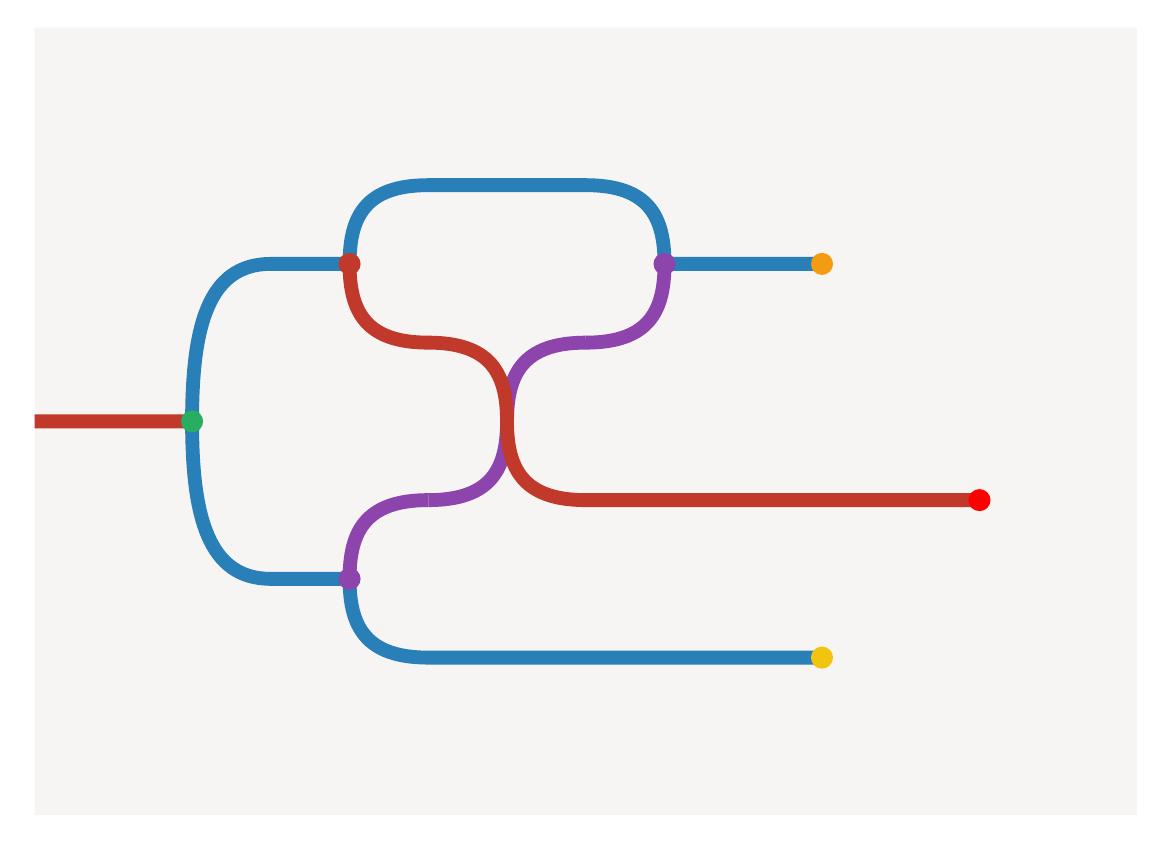
\begin{tikzpicture}
\definecolor{generator-13-5-0-pos}{RGB}{192, 57, 43}
\definecolor{generator-9-4-0-pos}{RGB}{142, 68, 173}
\definecolor{generator-1-4-0-pos}{RGB}{192, 57, 43}
\definecolor{generator-6-5-0-pos}{RGB}{243, 156, 18}
\definecolor{generator-5-5-0-pos}{RGB}{241, 196, 15}
\definecolor{generator-12-5-0-pos}{RGB}{142, 68, 173}
\definecolor{generator-4-5-0-pos}{RGB}{39, 174, 96}
\definecolor{generator-11-5-0-pos}{RGB}{142, 68, 173}
\definecolor{generator-0-0-0-pos}{RGB}{246, 245, 244}
\definecolor{generator-3-5-0-pos}{RGB}{255, 0, 0}
\definecolor{generator-2-4-0-pos}{RGB}{41, 128, 185}
\begin{scope}
% Background surfaces
\fill[generator-0-0-0-pos] (0,-0) -- (0,-10) -- (14,-10) -- (14,-0) -- (0,-0);
% Wire layers
\draw[color=generator-9-4-0-pos, line width=5pt](5,-6) .. controls (5.8,-6) and (6,-5.6) .. (6,-5) .. controls (6,-4.4) and (6.2,-4) .. (7,-4);
\draw[color=generator-1-4-0-pos, line width=5pt](0,-5) -- (2,-5)(4,-3) .. controls (4,-3.6) and (4.2,-4) .. (5,-4) .. controls (5.8,-4) and (6,-4.4) .. (6,-5) .. controls (6,-5.6) and (6.2,-6) .. (7,-6) -- (12,-6);
\draw[color=generator-9-4-0-pos, line width=5pt](4,-7) .. controls (4,-6.4) and (4.2,-6) .. (5,-6)(7,-4) .. controls (7.8,-4) and (8,-3.6) .. (8,-3);
\draw[color=generator-2-4-0-pos, line width=5pt](2,-5) .. controls (2,-3.8) and (2.2,-3) .. (3,-3) -- (4,-3) .. controls (4,-2.4) and (4.2,-2) .. (5,-2) -- (7,-2) .. controls (7.8,-2) and (8,-2.4) .. (8,-3) -- (10,-3)(2,-5) .. controls (2,-6.2) and (2.2,-7) .. (3,-7) -- (4,-7) .. controls (4,-7.6) and (4.2,-8) .. (5,-8) -- (10,-8);
\end{scope}
\fill[generator-4-5-0-pos] (2,-5) circle (0.14);
\fill[generator-13-5-0-pos] (4,-3) circle (0.14);
\fill[generator-12-5-0-pos] (4,-7) circle (0.14);
\fill[generator-11-5-0-pos] (8,-3) circle (0.14);
\fill[generator-6-5-0-pos] (10,-3) circle (0.14);
\fill[generator-5-5-0-pos] (10,-8) circle (0.14);
\fill[generator-3-5-0-pos] (12,-6) circle (0.14);
\end{tikzpicture}
\]
\[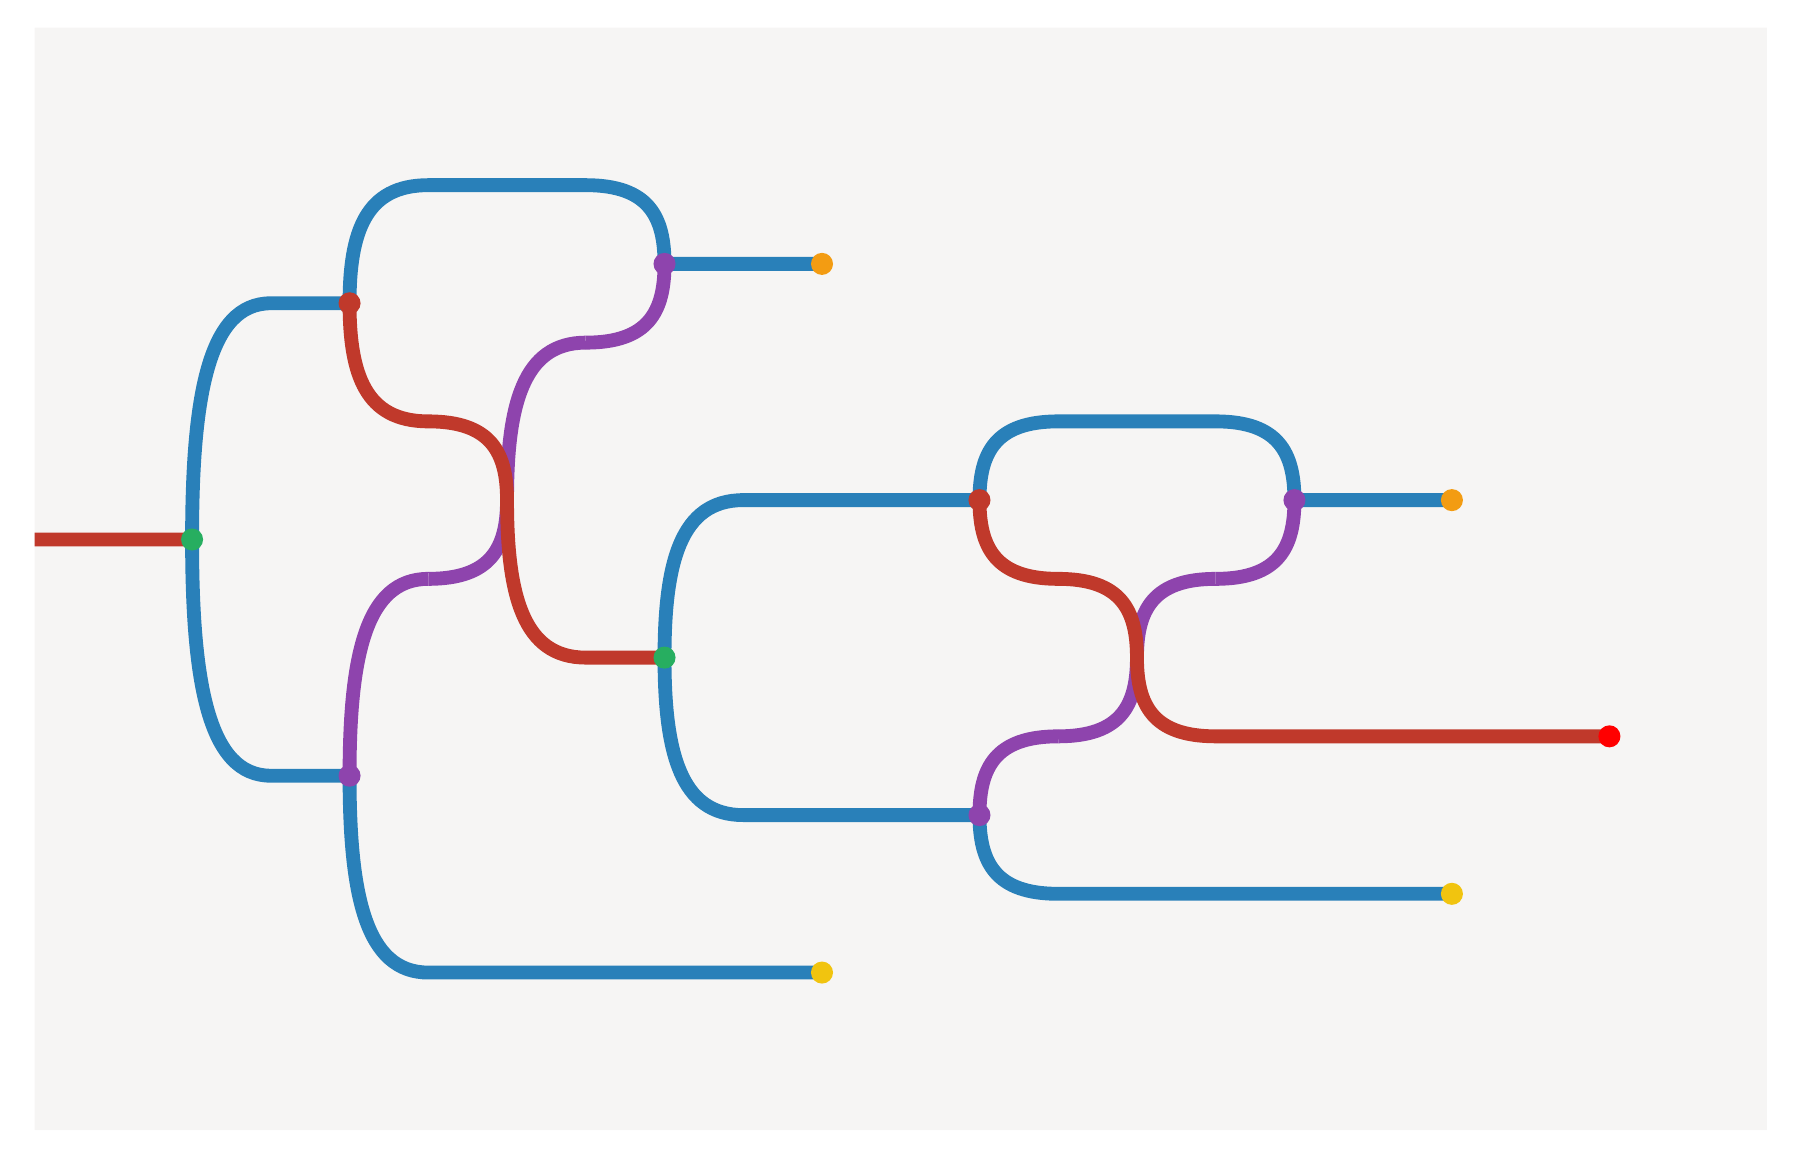
\begin{tikzpicture}
\definecolor{generator-13-5-0-pos}{RGB}{192, 57, 43}
\definecolor{generator-9-4-0-pos}{RGB}{142, 68, 173}
\definecolor{generator-1-4-0-pos}{RGB}{192, 57, 43}
\definecolor{generator-6-5-0-pos}{RGB}{243, 156, 18}
\definecolor{generator-5-5-0-pos}{RGB}{241, 196, 15}
\definecolor{generator-12-5-0-pos}{RGB}{142, 68, 173}
\definecolor{generator-4-5-0-pos}{RGB}{39, 174, 96}
\definecolor{generator-11-5-0-pos}{RGB}{142, 68, 173}
\definecolor{generator-0-0-0-pos}{RGB}{246, 245, 244}
\definecolor{generator-3-5-0-pos}{RGB}{255, 0, 0}
\definecolor{generator-2-4-0-pos}{RGB}{41, 128, 185}
\begin{scope}
% Background surfaces
\fill[generator-0-0-0-pos] (0,-0) -- (0,-14) -- (22,-14) -- (22,-0) -- (0,-0);
% Wire layers
\draw[color=generator-9-4-0-pos, line width=5pt](5,-7) .. controls (5.8,-7) and (6,-6.6) .. (6,-6) .. controls (6,-4.8) and (6.2,-4) .. (7,-4)(13,-9) .. controls (13.8,-9) and (14,-8.6) .. (14,-8) .. controls (14,-7.4) and (14.2,-7) .. (15,-7);
\draw[color=generator-1-4-0-pos, line width=5pt](0,-6.5) -- (2,-6.5)(4,-3.5) .. controls (4,-4.4) and (4.2,-5) .. (5,-5) .. controls (5.8,-5) and (6,-5.4) .. (6,-6) .. controls (6,-7.2) and (6.2,-8) .. (7,-8) -- (8,-8)(12,-6) .. controls (12,-6.6) and (12.2,-7) .. (13,-7) .. controls (13.8,-7) and (14,-7.4) .. (14,-8) .. controls (14,-8.6) and (14.2,-9) .. (15,-9) -- (20,-9);
\draw[color=generator-9-4-0-pos, line width=5pt](4,-9.5) .. controls (4,-8) and (4.2,-7) .. (5,-7)(7,-4) .. controls (7.8,-4) and (8,-3.6) .. (8,-3)(12,-10) .. controls (12,-9.4) and (12.2,-9) .. (13,-9)(15,-7) .. controls (15.8,-7) and (16,-6.6) .. (16,-6);
\draw[color=generator-2-4-0-pos, line width=5pt](2,-6.5) .. controls (2,-4.7) and (2.2,-3.5) .. (3,-3.5) -- (4,-3.5) .. controls (4,-2.6) and (4.2,-2) .. (5,-2) -- (7,-2) .. controls (7.8,-2) and (8,-2.4) .. (8,-3) -- (10,-3)(2,-6.5) .. controls (2,-8.3) and (2.2,-9.5) .. (3,-9.5) -- (4,-9.5) .. controls (4,-11) and (4.2,-12) .. (5,-12) -- (10,-12)(8,-8) .. controls (8,-6.8) and (8.2,-6) .. (9,-6) -- (12,-6) .. controls (12,-5.4) and (12.2,-5) .. (13,-5) -- (15,-5) .. controls (15.8,-5) and (16,-5.4) .. (16,-6) -- (18,-6)(8,-8) .. controls (8,-9.2) and (8.2,-10) .. (9,-10) -- (12,-10) .. controls (12,-10.6) and (12.2,-11) .. (13,-11) -- (18,-11);
\end{scope}
\fill[generator-4-5-0-pos] (2,-6.5) circle (0.14);
\fill[generator-13-5-0-pos] (4,-3.5) circle (0.14);
\fill[generator-12-5-0-pos] (4,-9.5) circle (0.14);
\fill[generator-11-5-0-pos] (8,-3) circle (0.14);
\fill[generator-4-5-0-pos] (8,-8) circle (0.14);
\fill[generator-6-5-0-pos] (10,-3) circle (0.14);
\fill[generator-5-5-0-pos] (10,-12) circle (0.14);
\fill[generator-13-5-0-pos] (12,-6) circle (0.14);
\fill[generator-12-5-0-pos] (12,-10) circle (0.14);
\fill[generator-11-5-0-pos] (16,-6) circle (0.14);
\fill[generator-6-5-0-pos] (18,-6) circle (0.14);
\fill[generator-5-5-0-pos] (18,-11) circle (0.14);
\fill[generator-3-5-0-pos] (20,-9) circle (0.14);
\end{tikzpicture}
\]
\[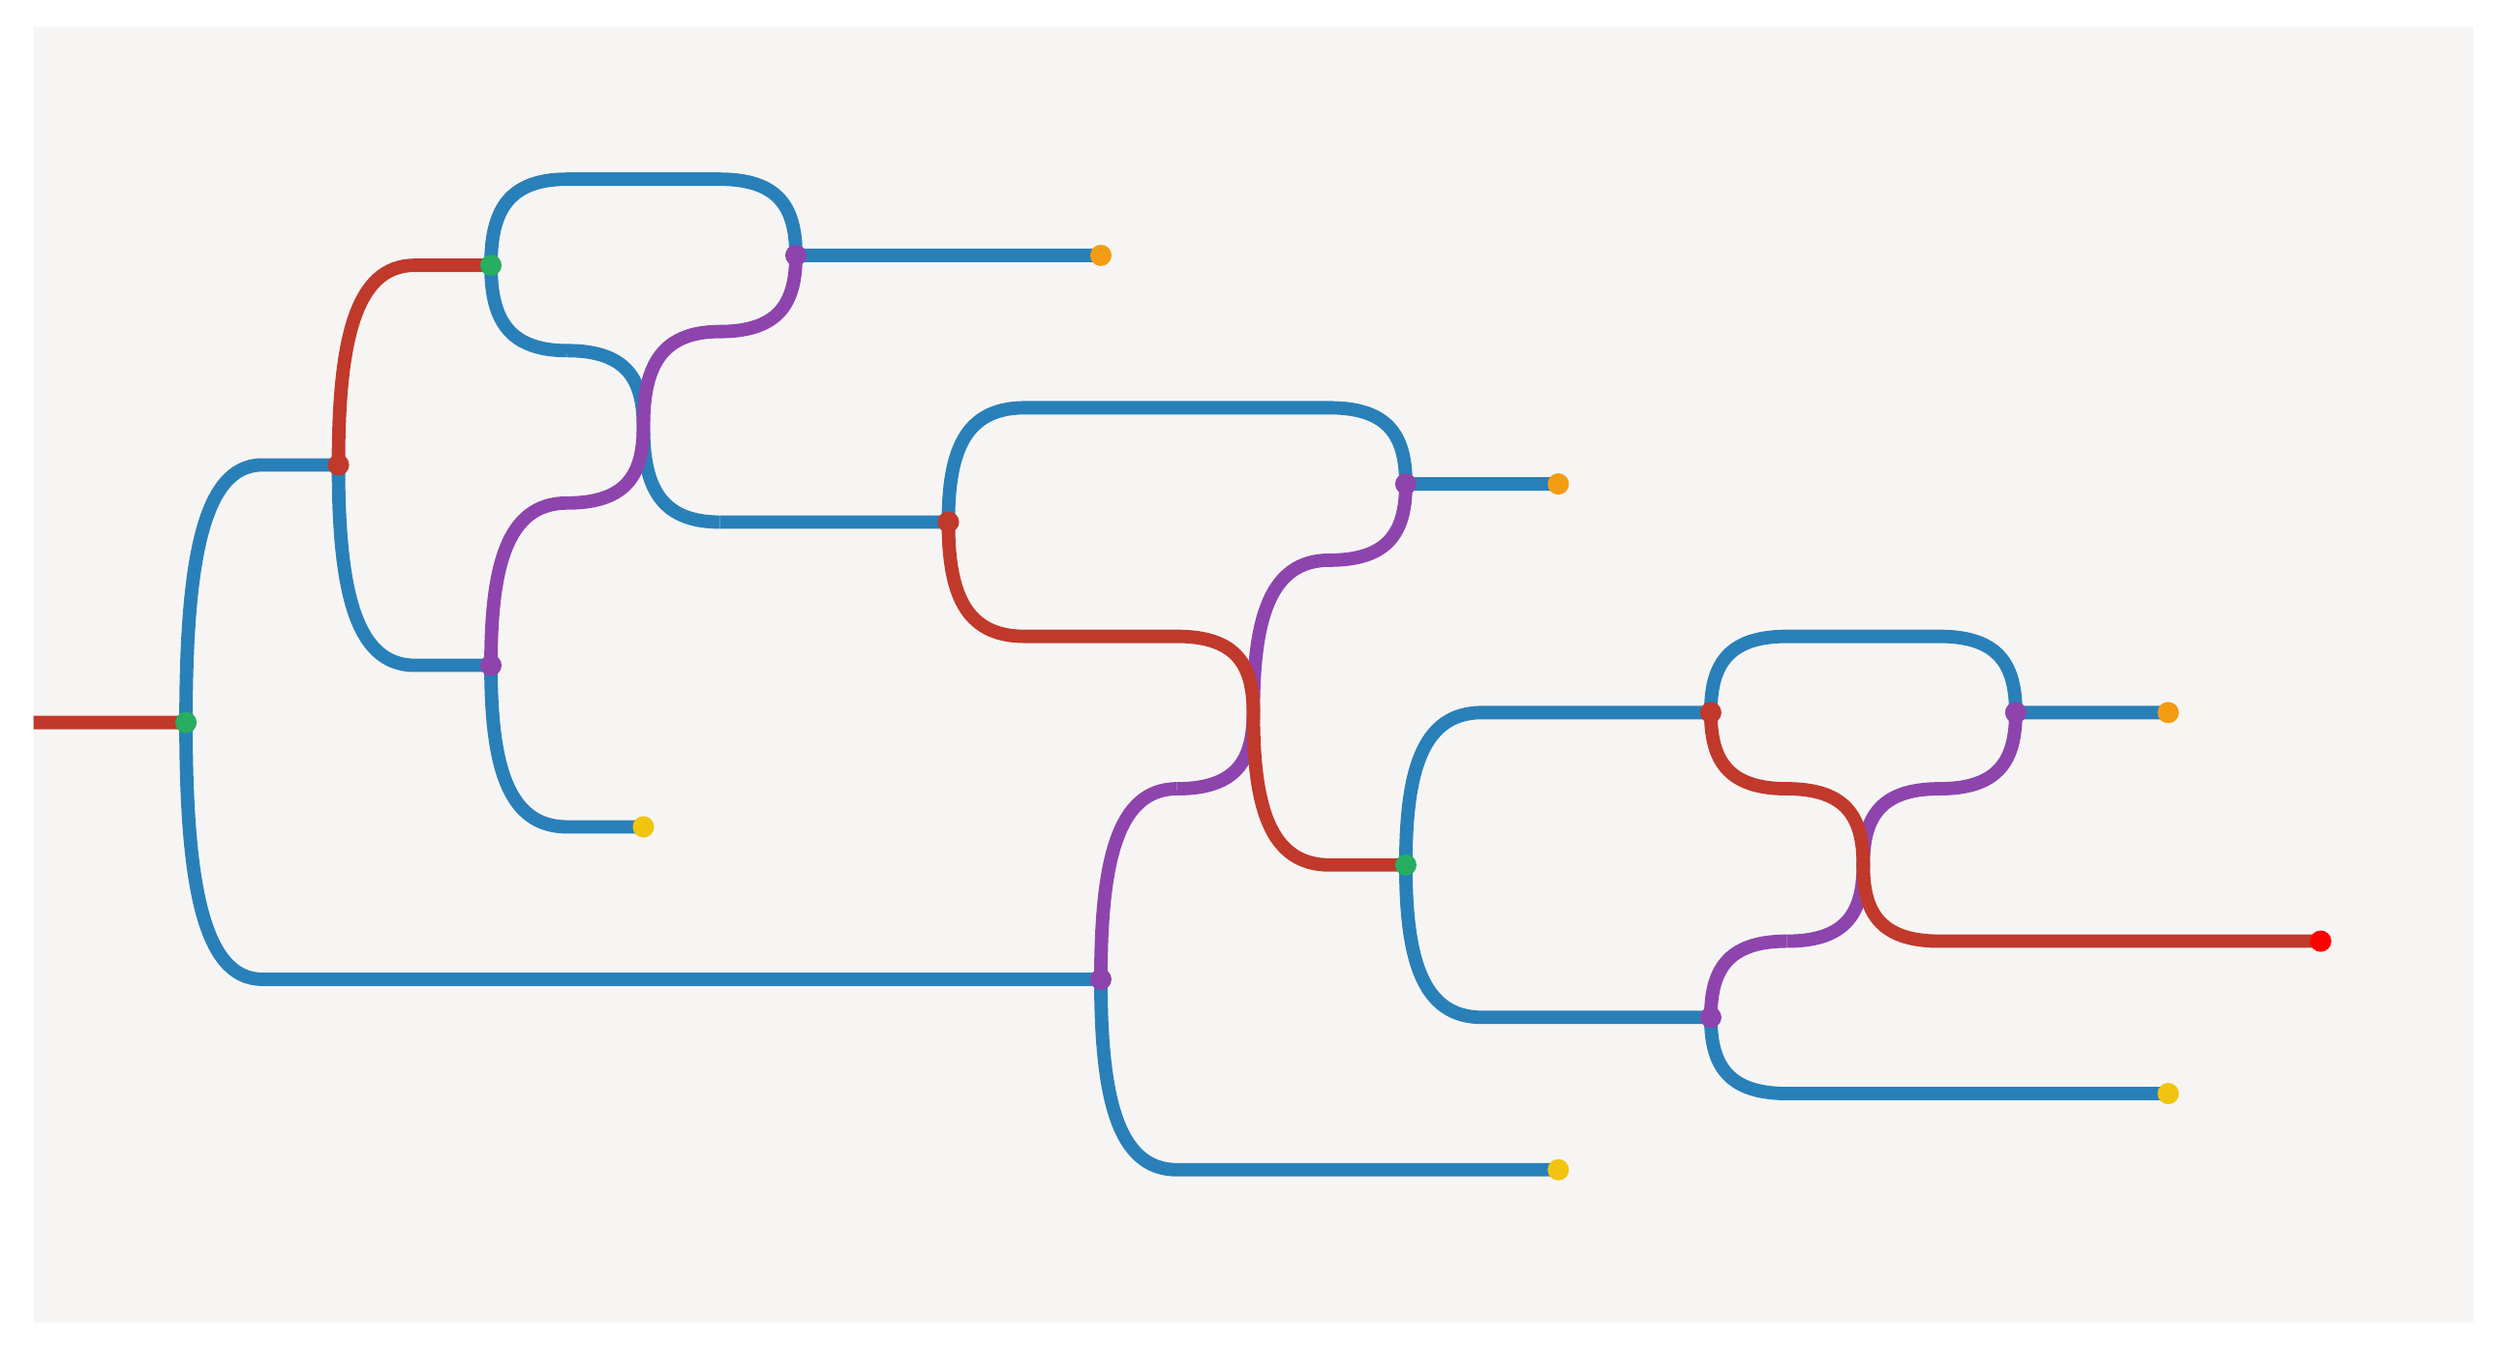
\begin{tikzpicture}
\definecolor{generator-13-5-0-pos}{RGB}{192, 57, 43}
\definecolor{generator-9-4-0-pos}{RGB}{142, 68, 173}
\definecolor{generator-1-4-0-pos}{RGB}{192, 57, 43}
\definecolor{generator-5-5-0-pos}{RGB}{241, 196, 15}
\definecolor{generator-6-5-0-pos}{RGB}{243, 156, 18}
\definecolor{generator-12-5-0-pos}{RGB}{142, 68, 173}
\definecolor{generator-8-5-0-pos}{RGB}{192, 57, 43}
\definecolor{generator-4-5-0-pos}{RGB}{39, 174, 96}
\definecolor{generator-11-5-0-pos}{RGB}{142, 68, 173}
\definecolor{generator-0-0-0-pos}{RGB}{246, 245, 244}
\definecolor{generator-3-5-0-pos}{RGB}{255, 0, 0}
\definecolor{generator-2-4-0-pos}{RGB}{41, 128, 185}
\begin{scope}
% Background surfaces
\fill[generator-0-0-0-pos] (0,-0) -- (0,-17) -- (32,-17) -- (32,-0) -- (0,-0);
% Wire layers
\draw[color=generator-9-4-0-pos, line width=5pt](15,-10) .. controls (15.8,-10) and (16,-9.6) .. (16,-9) .. controls (16,-7.8) and (16.2,-7) .. (17,-7)(23,-12) .. controls (23.8,-12) and (24,-11.6) .. (24,-11) .. controls (24,-10.4) and (24.2,-10) .. (25,-10);
\draw[color=generator-2-4-0-pos, line width=5pt](7,-4.25) .. controls (7.8,-4.25) and (8,-4.65) .. (8,-5.25) .. controls (8,-6) and (8.2,-6.5) .. (9,-6.5);
\draw[color=generator-1-4-0-pos, line width=5pt](0,-9.13) -- (2,-9.13)(4,-5.75) .. controls (4,-4.18) and (4.2,-3.13) .. (5,-3.13) -- (6,-3.13)(12,-6.5) .. controls (12,-7.4) and (12.2,-8) .. (13,-8) -- (15,-8) .. controls (15.8,-8) and (16,-8.4) .. (16,-9) .. controls (16,-10.2) and (16.2,-11) .. (17,-11) -- (18,-11)(22,-9) .. controls (22,-9.6) and (22.2,-10) .. (23,-10) .. controls (23.8,-10) and (24,-10.4) .. (24,-11) .. controls (24,-11.6) and (24.2,-12) .. (25,-12) -- (30,-12);
\draw[color=generator-9-4-0-pos, line width=5pt](6,-8.38) .. controls (6,-7.1) and (6.2,-6.25) .. (7,-6.25) .. controls (7.8,-6.25) and (8,-5.85) .. (8,-5.25) .. controls (8,-4.5) and (8.2,-4) .. (9,-4) .. controls (9.8,-4) and (10,-3.6) .. (10,-3)(14,-12.5) .. controls (14,-11) and (14.2,-10) .. (15,-10)(17,-7) .. controls (17.8,-7) and (18,-6.6) .. (18,-6)(22,-13) .. controls (22,-12.4) and (22.2,-12) .. (23,-12)(25,-10) .. controls (25.8,-10) and (26,-9.6) .. (26,-9);
\draw[color=generator-2-4-0-pos, line width=5pt](2,-9.13) .. controls (2,-7.1) and (2.2,-5.75) .. (3,-5.75) -- (4,-5.75) .. controls (4,-7.33) and (4.2,-8.38) .. (5,-8.38) -- (6,-8.38) .. controls (6,-9.65) and (6.2,-10.5) .. (7,-10.5) -- (8,-10.5)(2,-9.13) .. controls (2,-11.15) and (2.2,-12.5) .. (3,-12.5) -- (14,-12.5) .. controls (14,-14) and (14.2,-15) .. (15,-15) -- (20,-15)(6,-3.13) .. controls (6,-2.45) and (6.2,-2) .. (7,-2) -- (9,-2) .. controls (9.8,-2) and (10,-2.4) .. (10,-3) -- (14,-3)(6,-3.13) .. controls (6,-3.8) and (6.2,-4.25) .. (7,-4.25)(9,-6.5) -- (12,-6.5) .. controls (12,-5.6) and (12.2,-5) .. (13,-5) -- (17,-5) .. controls (17.8,-5) and (18,-5.4) .. (18,-6) -- (20,-6)(18,-11) .. controls (18,-9.8) and (18.2,-9) .. (19,-9) -- (22,-9) .. controls (22,-8.4) and (22.2,-8) .. (23,-8) -- (25,-8) .. controls (25.8,-8) and (26,-8.4) .. (26,-9) -- (28,-9)(18,-11) .. controls (18,-12.2) and (18.2,-13) .. (19,-13) -- (22,-13) .. controls (22,-13.6) and (22.2,-14) .. (23,-14) -- (28,-14);
\end{scope}
\fill[generator-4-5-0-pos] (2,-9.13) circle (0.14);
\fill[generator-8-5-0-pos] (4,-5.75) circle (0.14);
\fill[generator-4-5-0-pos] (6,-3.13) circle (0.14);
\fill[generator-12-5-0-pos] (6,-8.38) circle (0.14);
\fill[generator-5-5-0-pos] (8,-10.5) circle (0.14);
\fill[generator-11-5-0-pos] (10,-3) circle (0.14);
\fill[generator-13-5-0-pos] (12,-6.5) circle (0.14);
\fill[generator-6-5-0-pos] (14,-3) circle (0.14);
\fill[generator-12-5-0-pos] (14,-12.5) circle (0.14);
\fill[generator-11-5-0-pos] (18,-6) circle (0.14);
\fill[generator-4-5-0-pos] (18,-11) circle (0.14);
\fill[generator-6-5-0-pos] (20,-6) circle (0.14);
\fill[generator-5-5-0-pos] (20,-15) circle (0.14);
\fill[generator-13-5-0-pos] (22,-9) circle (0.14);
\fill[generator-12-5-0-pos] (22,-13) circle (0.14);
\fill[generator-11-5-0-pos] (26,-9) circle (0.14);
\fill[generator-6-5-0-pos] (28,-9) circle (0.14);
\fill[generator-5-5-0-pos] (28,-14) circle (0.14);
\fill[generator-3-5-0-pos] (30,-12) circle (0.14);
\end{tikzpicture}
\]

\textbf{N.B.} In practice when using \texttt{homotopy.io} for the symmetric monoidal setting, it is simpler to suspend symmetric monoidal signatures to begin at 4-cells rather than 3-cells. The reason for this is that under- and over-braids still exist in the symmetric monoidal setting, and while sequentially composed braids are homotopically equivalent to the pair of identities, they are not uniquely so, thus these homotopies must be input manually. By beginning at 4-cells (or higher, due to the stabilisation hypothesis []), braid-eliminations are unique up to homotopy and can be performed more easily in the proof assistant.
\end{example}

Now we have enough to spell out full TAGs with local constraints and links as an $n$-categorical signature. To recap briefly, we have seen that we can model the passage from CFGs to TAGs in the $n$-categorical setting, and then how selective and null adjoining rules by specifying endomorphisms on wires as the source of rewrites, and finally that we can model links in the symmetric monoidal setting. Maintaining planarity (which is important for a left-to-right order of terminals for spelling out a language) and modelling obligatory rewrites can be done by requiring that \emph{finished} derivations are precisely those whose only twists are link-wires, and have no sources for obligatory adjoins.

\begin{defn}[Tree Adjoining Grammars with local constraints and links in \texttt{homotopy.io}]

A \emph{Linguistic Tree Adjoining Grammar} is given by the following data:

\[(\mathcal{N}, \mathcal{N}^\downarrow, \mathcal{N}^*, \Sigma, \mathcal{I}, \mathcal{A}, \mathfrak{S} \subseteq \mathcal{P}(\mathcal{A}), \Box, \Diamond, \mathfrak{L} \subseteq \mathcal{N})\]

The initial elements are the same as an elementary tree-adjoining grammar and obey the same constraints. The modifications are:

\begin{itemize}
\item{$\mathcal{I}$ is a nonempty set of \emph{initial} constrained-linked-trees.}
\item{$\mathcal{A}$ is a nonempty set of \emph{auxiliary} constrained-linked-trees.}
\item{$\mathfrak{S}$ is a set of sets of \emph{select} auxiliary trees.}
\item{$\Box, \Diamond$ are fresh symbols. $\Box$ marks \emph{obligatory adjoins}, and $\Diamond$ marks \emph{optional} adjoins.}
\item{$\mathfrak{L}$ is a set permissible \emph{link types} among nonterminals or $\top$.}
\end{itemize}
A \emph{constrained-linked-tree}, or CL-tree, is a pair consisting of:
\begin{itemize}
\item{A tree where each internal node is an element of $\mathcal{N} \times \mathfrak{S} \times \{\Box,\Diamond\} \times \{*, \bar{*}\}$, and each leaf is an element of $\mathcal{N} \times \mathfrak{S} \times \{\Box,\Diamond\} \times \{*, \bar{*}\} \cup \Sigma$. In prose, each label is either a terminal symbol (as a leaf), or otherwise a nonterminal, along with a subset of auxiliary trees that indicates select adjoins (or null-adjoins when the subset is $\varnothing$), a marker indicating whether those adjoins are obligatory or optional, and a marker indicating whether the node is a foot node or not. Observe that there is no need to indicate when a node is a valid target for substitution since that function is subsumed by null adjoining rules.}
\item{
A set of ordered pairs of nodes $(n_1,n_2)$ of the tree such that:
\begin{enumerate}
\item{$n_2$ \emph{c-commands} $n_1$, (i.e., $n_2$ is not an ancestor of $n_1$, and there exists a node $m$ which is the immediate parent node of $n_2$, and an ancestor of $n_1$).}
\item{$n_1$ and $n_2$ share the same type $\mathbf{T} \in \mathcal{N}$ and $\mathbf{T} \in \mathfrak{L}$, or both $n_1,n_2$ are terminals.}
\item{$n_1$ is the parent of terminal symbols, or childless.}
\end{enumerate}
}
\end{itemize}

We spell out how this data becomes an $n$-categorical signature by enumerating cell dimensions:

\begin{enumerate}
\setcounter{enumi}{-1}
\item{A single object $\star$}
\item{None.}
\item{None.}
\item{
	\begin{itemize}
	\item{For each $\mathbf{T} \in \mathcal{N}$, a cell $\mathbf{T}: \mathbf{1}_{\mathbf{1}_\star} \rightarrow \mathbf{1}_{\mathbf{1}_\star}$.}
	\item{$\top: \mathbf{1}_{\mathbf{1}_\star} \rightarrow \mathbf{1}_{\mathbf{1}_\star}$ A wire for terminal symbols.}
	\item{For each $\mathbf{L} \in \mathfrak{L}$, a cell $\mathbf{L} : \mathbf{1}_{\mathbf{1}_\star} \rightarrow \mathbf{1}_{\mathbf{1}_\star}$.}
	\end{itemize}
}
\item{
	We distinguish between \emph{atomic} and \emph{composite} generators at this level. The trees themselves are composites of \emph{atomic} generators. The \emph{atomic} generators are:
	\begin{itemize}
	\item{For each node $n$ that occurs in either $\mathcal{I}$ or $\mathcal{A}$, we populate cells by a case analysis:
	\begin{itemize}
		\item{If $n$ is a terminal $\sigma \in \Sigma$, we create a cell $\sigma: \top \rightarrow \mathbf{1}_{\mathbf{1}_{\mathbf{1}_\star}}$.}
		\item{If $n = (\mathbf{T},\mathbf{S},\dagger,\bar{*})$, we create $\mathbf{S}_\mathbf{T}^\Box: \mathbf{T} \rightarrow \mathbf{T}$ if the node is marked obligatory ($\dagger = \Box$), and a cell $\mathbf{S}_\mathbf{T}^\Diamond: \mathbf{T} \rightarrow \mathbf{T}$ otherwise.}
		\item{If $n = (\mathbf{T},\mathbf{S},\dagger,*)$, it is a foot note, for which we create a cell $\mathbf{S}_\mathbf{T}^\Box: \mathbf{T} \rightarrow \mathbf{1}_{\mathbf{1}_{\mathbf{1}_\star}}$ if the node is marked obligatory ($\dagger = \Box$), and a cell $\mathbf{S}_\mathbf{T}^\Diamond: \mathbf{T} \rightarrow \mathbf{1}_{\mathbf{1}_{\mathbf{1}_\star}}$ otherwise.}
	\end{itemize}
	}
	\item{For each $\mathbf{L} \in \mathfrak{L}$ (which is also a type $\mathbf{T} \in \mathcal{N}$) a pair of cells $\mathbf{T}^\mathbf{L} := \mathbf{T} \rightarrow \mathbf{T} \otimes \mathbf{L}$ and $\mathbf{T}_\mathbf{L} := \mathbf{L} \otimes \mathbf{T} \rightarrow \mathbf{T}$.}
	\item{For each node $p$ of type $\mathbf{T}_p$ in either $\mathcal{I}$ or $\mathcal{A}$ with a nonempty left-to-right list of children $C_p := <c_1,c_2,\cdots c_i, c\dots c_n>$ with types $\mathbf{T}_i$, a branch cell $C_p : \mathbf{T}_p \rightarrow \bigotimes\limits_{i=1}^{n} \mathbf{T}_i$.}
	\end{itemize}
	We represent trees by composite generators, defined recursively. For a given tree $\mathcal{T}$ in either $\mathcal{I}$ or $\mathcal{A}$, we define a composite generator beginning at the root. Where the root node is $p = (\mathbf{T},\mathbf{S},\dagger)$, we begin with the cell $\mathbf{S}_\mathbf{T}^\dagger$. For branches, we compose the branch cell $C_p$ to this cell sequentially. If $p$ has a child $c$ that has a link, we do a case analysis. If that child c-commands the other end of the link we generate the first half of the linking wire by composing $\mathbf{T}^\mathbf{L}$ for the appropriate type $\mathbf{T}$ of the child node. Otherwise the child is c-commanded by a previously generated link, which we braid over and connect using $\mathbf{T}_\mathbf{L}$, again with the appropriate typing for the child. Now we may recurse the procedure for subtrees. If a node has no children, it is a leaf $l = (\mathbf{T},\mathbf{S},\dagger)$ or a terminal symbol. We append a terminal cell $\sigma$ if $l$ is a terminal symbol (thus killing the wire), and otherwise we leave an open $\mathbf{T}$ wire after appending $\mathbf{S}_\mathbf{T}^\dagger$. Altogether this obtains a 3-cell which we denote $\mathcal{T}$, overloading notation; different execution-orders of the above procedure evidently obtain 3-cells equivalent up to homotopy.
}
\item{}
\end{enumerate}

\end{defn}\label{sec:ncat}
\clearpage
\newpage
\newpage

\section{A generative grammar for text circuits}

\subsection{A circuit-growing grammar}

\marginnote{
\begin{defn}[Lexicon]\label{defn:lex}
We define a limited lexicon $\mathcal{L}$ to be a tuple of disjoint finite sets $(\mathbf{N}, \mathbf{V}_1, \mathbf{V}_2, \mathbf{V}_{\texttt{S}}, \mathbf{A}_{\texttt{N}}, \mathbf{A}_{\texttt{V}}, \mathbf{C})$
\end{defn}
}

\marginnote{
Where:
\begin{itemize}
\item $\mathbf{N}$ is a set of \emph{proper nouns}
\item $\mathbf{V}_1$ is a set of \emph{intransitive verbs}
\item $\mathbf{V}_2$ is a set of \emph{transitive verbs}
\item $\mathbf{V}_{\texttt{S}}$ is a set of \emph{sentential-complement verbs}
\item $\mathbf{A}_{\texttt{N}}$ is a set of \emph{adjectives}
\item $\mathbf{A}_{\texttt{V}}$ is a set of \emph{adverbs}
\item $\mathbf{C}$ is a set of \emph{conjunctions}
\end{itemize}
}

\begin{marginfigure}
\centering
\[
\resizebox{\textwidth}{!}{\tikzfig{mushroom/howtoread}}
\]
\caption{\textbf{How to read the diagrams in this section:} we will be making heavy use of pink and purple bubbles as frames to construct circuits. We will depict the bubbles horizontally, as we are permitted to by compact closure, or by reading diagrams with slightly skewed axes.}
\end{marginfigure}

There are many different ways to write a weak $n$-categorical signature that generates circuits. Mostly as an illustration of expressivity, I will provide a signature where the terms "surface" and "deep" structure are taken literally as metaphors; the generative grammar will grow a line of words in syntactic order, and like mushrooms on soil, the circuits will behave as the mycelium underneath the words. It won't be the most efficient way to do it in terms of the number of rules to consider, but it will look nice and we'll be able to reason about it easily.\\

\newthought{Simplifications and limitations}: For now we only consider word types as in Definition \ref{defn:lex}, though we will see how to engineer extensions later. We only deal with propositional statements, without determiners, in only one tense, with no morphological agreement between nouns and their verbs and referring pronouns, and we assume that adverbs, adjectives stack indefinitely and without further order requirements: e.g. \texttt{Alice happily secretly finds red big toy shiny car that he gives to Bob} is a sentence we consider grammatical enough. For now, we consider only the case where adjectives and adverbs appear before their respective noun or verb. Note that all of these limitations apart from the limited lexicon can principle be overcome by the techniques we developed in Section \ref{sec:ncat} for restricted tree-adjoining and links. As a historical remark, generative-transformational grammars fell out of favour linguistically due to the problem of overgeneration: the generation of nonsense or unacceptable sentences in actual language use. We're undergenerating and overgenerating at the same time, but we're also not concerned with empirical capture: we only require a concrete mathematical basis to build interesting things on top of. On a related note, there's zero chance that this particular circuit-growing grammar even comes close to how language is actually produced by humans, and I have no idea whether a generalised graph-rewriting approach is cognitively realistic.

\newthought{Mathematical assumptions}: We work in a dimension where wires behave symmetric monoidally by homotopy, and further assume strong compact closure rewrite rules for all wire-types. Our strategy will be to generate "bubbles" for sentences, within which we can grow circuit structure piecemeal. We will only express the rewrite rules; the generators of lower dimension are implicit. We aim to recover the linear ordering of words in text (essential to any syntax) by traversing the top surface of a chain of bubbles representing sentence structure in text -- this order will be invariant up to compact closed isomorphisms. The diagrammatic consequence of these assumptions is that we will be working with a conservative generalisation of graph-rewriting defined by local rewriting rules. The major distinction is that locality can be redefined up to homotopy, which allows locally-defined rules to operate in what would be a nonlocal fashion in terms of graph neighbourhoods, as in Figure \ref{fig:locality}. The minor distinction is that rewrite rules are sensitive to twists in wires and the radial order in which wires emanate from nodes, though it is easy to see how these distinctions can be circumvented by additional by imposing the equivalent of commutativity relations as bidirectional rewrites. It is worth remarking that one can devise weak n-categorical signatures to simulate turing machines, where output strings are e.g. 0-cells on a selected 1-cell, so rewrite systems of the kind we propose here are almost certainly expressively sufficient for anything; the real benefit is the interpretable geometric intuitions of the diagrams.

\begin{figure}[h!]\label{fig:locality}
\centering
\[
\resizebox{\textwidth}{!}{\tikzfig{mushroom/locality}}
\]
\caption{In this toy example, obtaining the same rewrite that connects the two yellow nodes with a purple wire using only graph-theoretically-local rewrites could potentially require an infinite family of rules for all possible configurations of pink and cyan nodes that separate the yellow, or would otherwise require disturbing other nodes in the rewrite process. In our setting, strong compact closure homotopies handle navigation between different spatial presentations so that a single rewrite rule suffices: the source and target notated by dotted-black circles. Despite the expressive economy and power of finitely presented signatures, we cannot "computationally cheat" graph isomorphism: formally we must supply the compact-closure homotopies as part of the rewrite, absorbed and hidden here by the $\simeq$ notation.}
\end{figure}

\newthought{The plan}: We start with simple sentences that only contain a single intransitive or transitive verb. Then we consider more general sentences. For these two steps, we characterise the expressive capacity of our rules in terms of a context-sensitive grammar that corresponds to the surface structure of the derivations. Then we introduce text structure as lists of sentences with coreferential structure on nouns, along with a mathematical characterisation of coreferential structure and a completeness result of our rules with respect to them. Then we (re)state and prove the text circuit theorem: that the fragment of language we have built with the syntax surjects onto text circuits. Finally we examine how we may model extensions to the expressive capacity of text circuits by introduction of new rewrite rules.

\clearpage

\subsection{Simple sentences}

\marginnote{
\begin{defn}[CSG for simple sentences]\label{dfn:simpCSG}
We may gauge the expressivity of simple sentences with the following context sensitive grammar.
\end{defn}
}

\marginnote{For verbs, adjectives, and modifiers, depicted unsaturated nouns as dotted and saturated with solid black lines, we have:
\[
\resizebox{\marginparwidth}{!}{\tikzfig{mushroom/simpleCFG}}
\]
}

\marginnote{
Adpositions require several helper-generators; we depict for example the beginning of the sequence of derivations that result from appending adpositions to an intransitive verb (the generators are implicit in the derivations):
\[
\resizebox{0.75\marginparwidth}{!}{\tikzfig{mushroom/simpleADP}}
\]
}

\marginnote{
\begin{proposition}\label{prop:simpsent}
Up to labels, the simple-sentence rules yield the same simple sentences as the CSG for simple sentences.
\begin{proof}
By graphical correspondence; viewing nodes on the pink surface as 1-cells, each rewrite rule yields a 2-cell. For example, for the \textcolor{green}{\texttt{IV}}-intro:
\[
\resizebox{0.5\marginparwidth}{!}{\tikzfig{mushroom/simpcorr}}
\]
\end{proof}
\end{proposition}
}

Simple sentences are sentences that only contain a single intransitive or transitive verb. Simple sentences will contain at least one noun, and may optionally contain adjectives, adverbs, and adpositions. The rules for generating simple sentences are as follows:

\[
\resizebox{\textwidth}{!}{\tikzfig{mushroom/simplesentences}}
\]

The $\texttt{N}_\uparrow$-intro rule introduces new unsaturated nouns from the end of a simple sentence. The \textcolor{green}{\texttt{IV}}-intro rule applies when there is precisely one unsaturated noun in the sentence, and the \textcolor{green}{\texttt{TV}}-intro rule applies when there are precisely two. Both verb-introduction rules saturate their respective nouns, which we depict with a black bulb. Adjectives may be introduced immediately preceding saturated nouns, and adverbs may be introduced immediately preceding any kind of verb. The position of adpositions in English is context-sensitive. To capture this, the $\textcolor{blue}{\texttt{ADP}}_{\textcolor{green}{\texttt{V}}}$-tendril rule allows an unsaturated adposition to appear immediately after a verb; a bulb may travel by homotopy to the right, seeking an unsaturated noun. Conversely, the bidirectional $\textcolor{blue}{\texttt{ADP}}_{\texttt{N}}$-tendril rule sends a mycelic tendril to the left, seeking a verb. The two pass-rules allow unsaturated adpositions to swap past saturated nouns and adjectives; note that by construction, neither verbs nor adverbs will appear in a simple sentence to the right of a verb, so unsaturated adpositions will move right until encountering an unsaturated noun. In case it doesn't, the tendril- and pass- rules are bidirectional and reversible.

\clearpage

\subsection{Complex sentences}

Now we consider two refinements; conjunctions, and verbs that take sentential complements. we may have two sentences joined by a conjunction, e.g. \texttt{Alice dances \underline{while} Bob drinks}. We may also have verbs that take a sentential complement rather than a noun phrase, e.g. \texttt{Alice \underline{sees} Bob dance}; these verbs require nouns, which we depict as wires spanning bubbles.

\begin{figure}[h!]\label{fig:sentbestiary}
\centering
\[
\resizebox{\textwidth}{!}{\tikzfig{mushroom/Sbestiary}}
\]
\caption{The dotted-blue wires do not contentfully interact with anything else; they will serve as visual aids for circuit-translation later, to indicate the contents of boxes. They do however indicate a diagrammatic strategy for extensions to accommodate noun phrases, to be explored later.}
\end{figure}

\marginnote{
\begin{defn}[Sentence structure]\label{dfn:sentCSG}
A sentence can be:
\begin{itemize}
\item a simple sentence, which...
\item ... may generate unsaturated nouns from the right.
\item a pair of sentences with a conjunction in between.
\item (if there is a single unsaturated noun) a sentence with a sentential-complement verb that scopes over a sentence.
\end{itemize}
As a CSG, these considerations are respectively depicted as:
\end{defn}
\[
\resizebox{\marginparwidth}{!}{\tikzfig{mushroom/complexsentenceCSG}}
\]
}

\marginnote{
\begin{proposition}\label{prop:compsent}
Up to labels, the rules so far yield the same sentences as the combined CSG of Definitions \ref{dfn:simpCSG} and \ref{dfn:sentCSG}.
\begin{proof}
Same correspondence as Proposition \ref{prop:simpsent}, ignoring the dotted-blue guards.
\end{proof}
\end{proposition}
}

\begin{figure}[h!]\label{fig:soberA}
\centering
\[
\resizebox{\textwidth}{!}{\tikzfig{mushroom/soberA}}
\]
\caption{
\begin{example}[\texttt{sober} $\alpha$ \texttt{sees drunk} $\beta$ \texttt{clumsily dance.}]
Now we can see our rewrites in action for sentences. As a matter of convention -- reflected in how the various pass- rules do not interact with labels -- we assume that labelling occurs after all of the words are saturated. We have still not introduced rules for labelling nouns: we delay their consideration until we have settled coreferential structure. For now they are labelled informally with greeks.
\end{example}
}
\end{figure}

\begin{figure}[h!]\label{fig:Alaughs}
\centering
\[
\resizebox{\textwidth}{!}{\tikzfig{mushroom/Alaughs}}
\]
\caption{
\begin{example}[$\alpha$ \texttt{laughs at} $\beta$]
Adpositions form by first sprouting and connecting tendrils under the surface. Because the tendril- and pass- rules are bidirectional, extraneous tendrils can always be retracted, and failed attempts for verbs to find an adpositional unsaturated noun argument can be undone. Though this seems computationally wasteful, it is commonplace in generative grammars to have the grammar overgenerate and later define the set of sentences by restriction, which is reasonable so long as computing the restriction is not computationally hard. In our case, observe that once a verb has been introduced and its argument nouns have been saturated, only the introduction of adpositions can saturate additionally introduced unsaturated nouns. Therefore we may define the finished sentences of the circuit-growing grammar to be those that e.g. contain no unsaturated nodes on the surface, which is a very plausible linear-time check by traversing the surface.
\end{example}
}
\end{figure}

\clearpage

\subsection{Text structure and noun-coreference}

\begin{figure}[h!]
\centering
\[
\tikzfig{mushroom/sintro}
\]
\caption{Only considering words, text is just a list of sentences. However, for our purposes, text additionally has \emph{coreferential structure}. Ideally, we would like to connect "the same noun" from distinct sentences as we would circuits.}
\end{figure}

\begin{figure}[h!]
\centering
\[
\tikzfig{mushroom/circuitplan}
\]
\caption{We choose the convention of connecting from left-to-right and from bottom-to-top, so that we might read circuits as we would text: the components corresponding to words will be arranged left-to-right and top-to-bottom. Connecting nouns across distinct sentences presents no issue, but a complication arises when connecting nouns within the same sentence as with reflexive pronouns e.g. \texttt{Alice likes herself}.}
\end{figure}

\begin{figure}[h!]\label{fig:reflcomp}
\centering
\[
\tikzfig{mushroom/reflcomplication}
\]
\caption{Reflexive coreference would violate of the processivity condition of string diagrams for symmetric monoidal categories. Not all symmetric monoidal categories possess the appropriate structure to interpret such reflexive pronouns, but there exist interpretative options. From left to right in roughly decreasing stringency, compact closed categories are the most direct solution. More weakly, traced symmetric monoidal categories also suffice. If there are no traces, so long as the noun wire possesses a monoid and comonoid, a convolution works. If all else fails, one can just specify a new gate. We will define coreference structure to exclude such reflexive coreference and revisit the issue as an extension.}
\end{figure}

\newpage

Now we will deal with coreferential structure and noun-labels.
\begin{fullwidth}
\[
\resizebox{1.5\textwidth}{!}{\tikzfig{mushroom/nounbestiary_newnew}}
\]
\end{fullwidth}

The linked-\texttt{N}-intro rules introduce a new unsaturated noun in the next sentence that coreferences the noun in the previous sentence that generated it. The \texttt{N}-shift rules allow any unsaturated noun to move into the next sentence. For both of the previous rules, the $\beta$ variant handles the case where the next sentence is related to the first by a conjunction. Observe that nouns with a forward coreference have two dotted-black wires leaving the root of their wires, which distinguishes them from nouns that only have a backward coreference or no coreference at all, which only have a single dotted-black wire leaving the root of their wire.\\

The \texttt{N}-swap rule variants allow a unsaturated noun with no forward coreferences to swap places with any unsaturated noun that immediately succeeds it.\\

\begin{figure}[h!]\label{fig:nounkinds}
\centering
\[
\resizebox{\textwidth}{!}{\tikzfig{mushroom/nounkinds}}
\]
\caption{At this point, it is worth establishing some terminology about the kinds of unsaturated nouns we have in play. The kinds of nouns are distinguished by their tails. \emph{Lonely} nouns have no coreferences, their tails connect to nothing. \emph{Head} nouns have a forward coreference in text; they have two tails, one that connects to nothing and the other to a noun later in text. \emph{Middle} nouns have a forward and backward coreference; they have two tails, one that connects to a noun in some preceding sentence, and one that connects forward to a noun in a succeeding sentence. \emph{Foot} nouns only have a backward coreference; they have a single tail connecting to a noun in some preceding sentence.}
\end{figure}

\begin{proposition}\label{prop:linkedlist}
The unsaturated noun kinds listed in Figure \ref{fig:nounkinds} are exhaustive, hence nouns that share a coreference are organised as a diagrammatic linked-list.
\begin{proof}
The \texttt{N}-intro rule creates lonely nouns. Head nouns can only be created by the linked-\texttt{N}-intro applied to a lonely noun. Any new noun created by linked-\texttt{N}-intro is a foot noun. The linked-\texttt{N}-intro rule turns foot nouns into middle nouns. These two intro- rules are the only ones that introduce unsaturated nouns, so it remains to demonstrate that no other rules can introduce noun-kinds that fall outside our taxonomy. The \texttt{N}-shift rule changes relative position of either a lonely or foot noun but cannot change its kind. The \texttt{N}-swap rule may start with either a lonely or foot noun on the left and either a head or middle noun on the right, but the outcome of the rule cannot change the starting kinds as tail-arity is conserved.
\end{proof}
\end{proposition}

\begin{proposition}
Let the \emph{population} of unsaturated nouns in a diagram be the multiset of kinds with multiplicity of their occurence. The \texttt{N}-shift and \texttt{N}-swap rules keep the population invariant.
\begin{proof}
By the end of the argument in Proposition \ref{prop:linkedlist}, conservation of tail-arities by these two local rewrites cannot affect the population.
\end{proof}
\end{proposition}



The link-label rule is a (finite) family of rules parameterised by the nouns in the lexicon

\marginnote{
We require a definition of coreference structure in order verify that our rewrite rules are complete with respect to them. One reasonable constraint on coreference in text is that coreference always goes backwards. One way to express this constraint mathematically is the following:
\begin{defn}[Coreference structure]
In a text with $K \in \mathbb{N}$ distinct nouns and their coreferents, the linear order of noun+referents in a text corresponds to a list of positive integers that:
\begin{enumerate}
\item Starts with 1
\item Contains every $k \in [1\cdots K]$
\item For all $k \in [1 \cdots K]$, the head of the list up to the first occurence of $k$ contains all $j < k$.
\end{enumerate}
\end{defn}
}

\marginnote{
\begin{proposition}
The noun-introduction and manipulation rules are expressively complete with respect to coreference structure.
\begin{proof}

\end{proof}
\end{proposition}
}

\newpage

Nouns require verbs in order to be saturated. From left-to-right; if there is precisely one unlabelled noun, we may introduce an unlabelled intransitive verb and saturate the noun so that it is now ready to grow a label; or if there are two unlabelled nouns, we may introduce an unlabelled transitive verb on the surface and saturate the two nouns that will be subject and object; and verbs may be labelled.
\[
\tikzfig{mushroom/simpbestiary}
\]

\subsection{Modifiers}

Modifiers are optional parts of sentences that modify (and hence depend on there being) nouns and verbs. We consider adjectives, adverbs, and adpositions. From left to right; we allow adjectives to sprout immediately before a saturated noun, and we allow adverbs to sprout immediately before any verb.

\[
\tikzfig{mushroom/adjadv}
\]

Adpositions modify verbs by tying in an additional noun argument; e.g. while \texttt{runs} is intransitive, \texttt{runs towards} behaves as a transitive verb. Some more advanced technology is required to place adpositions and their thematic nouns in the correct linear order on the surface. In the left column; an adposition tendril can sprout from a verb via an unsaturated adposition, seeking an unsaturated noun to the right; an unsaturated noun can sprout an tendril seeking a verb to connect to on the left. Both of these rewrites are bidirectional, as tendrils might attempt connection but fail, and so be retracted. In the centre, when an unsaturated adposition and its tendril find an unsaturated noun, they may connect, saturating the adposition so that it is ready to label. In the right column; an unsaturated adposition may move past a saturated noun in the same sentence, which allows multiple adpositions for the same verb; finally, a saturated adposition can be labelled.

\[
\tikzfig{mushroom/adpbestiary}
\]

\subsection{Rewriting to circuit-form}

\newthought{Resolving references}

\[
\tikzfig{mushroom/pronbestiary}
\]

\[
\tikzfig{mushroom/pronres}
\]

\newthought{Connecting circuits}

\newpage
\subsection{Putting it all together}

\begin{figure}[h!]
\centering
\[
\resizebox{\textwidth}{!}{\tikzfig{mushroom/bigex1}}
\]
\caption{Starting from the initial sentence bubble, we generate a new sentence, introduce some nouns and an SCV, and then we connect our references at the bottom.}
\end{figure}

\begin{figure}[h!]
\centering
\[
\resizebox{\textwidth}{!}{\tikzfig{mushroom/bigex2}}
\]
\caption{Then we introduce intransitive verbs to saturate nouns, and we may also sprout some modifying adjectives and adverbs.}
\end{figure}

\begin{figure}[h!]
\centering
\[
\resizebox{\textwidth}{!}{\tikzfig{mushroom/bigex3}}
\]
\caption{For the remaining unsaturated noun, we use the adposition introduction rules to sprout tendrils off of the other verb in the bubble, and connect.}
\end{figure}

\begin{figure}[h!]
\centering
\[
\resizebox{\textwidth}{!}{\tikzfig{mushroom/bigex4}}
\]
\caption{All of the non-noun words may now be labelled.}
\end{figure}

\begin{figure}[h!]
\centering
\[
\resizebox{\textwidth}{!}{\tikzfig{mushroom/bigex5}}
\]
\caption{To begin assigning nouns, observe that by compact closure of the bubble boundaries, we can deform the diagram to obtain suitable forms for our local rewrite rules for link-generation at the bottom.}
\end{figure}

\begin{figure}[h!]
\centering
\[
\resizebox{\textwidth}{!}{\tikzfig{mushroom/bigex6}}
\]
\caption{Now we can introduce our noun labels and linearise our link structure.}
\end{figure}

\begin{figure}[h!]
\centering
\[
\resizebox{\textwidth}{!}{\tikzfig{mushroom/bigex7}}
\]
\caption{Once the link structure is linearised, we can undo the deformation, and propagate links to the surface.}
\end{figure}

\begin{figure}[h!]
\centering
\[
\resizebox{\textwidth}{!}{\tikzfig{mushroom/bigex8}}
\]
\caption{The bubbles may be rearranged to respect circuit-form, such that the propagation of noun labels to the surface traces out the wires of the end circuit.}
\end{figure}

\clearpage
\newpage
\subsection{Extensions I: relative and reflexive pronouns}

\newthought{Subject relative pronouns}

\begin{example}

\end{example}

\newthought{Object relative pronouns}

\begin{example}

\end{example}

\newthought{Reflexive pronouns}

\begin{example}

\end{example}

\subsection{Extensions II: grammar equations}

\newthought{Attributive vs. predicative modifiers}

\begin{example}

\end{example}

\newthought{Copulas}

\begin{example}

\end{example}

\newthought{Possessive pronouns}

\begin{example}

\end{example}

\subsection{Extensions III: higher-order modifiers}

\newthought{Intensifiers}

\begin{example}

\end{example}

\newthought{Comparatives}

\begin{example}

\end{example}

\subsection{Equivalence to internal wirings}

\subsection{Text circuit theorem}

\subsection{Related work}
\clearpage
\newpage
\section{Text circuits: details, demos, developments}\label{sec:circs}

\marginnote{An example from Task 1, "single supporting fact", is:\\
\[\texttt{Mary went to the bathroom.}\]
\[\texttt{John moved to the hallway.}\]
\[\texttt{Mary travelled to the office.}\]
\[\texttt{\textcolor{blue}{(Query:) Where is Mary?}}\]
\[\texttt{(Answer:) office.}\]
Translating the setup of each task into a circuit of neural nets-to-be-learnt, and queries into appropriately typed measurements-to-be-learnt, each bAbi task becomes a training condition in the form of a process-theoretic equation to be satisfied: the depicted composite process ought to be equal to the \texttt{office} state:
\[
\resizebox{0.4\textwidth}{!}{\tikzfig{textcirc/babiex}}
\]
}

This section covers some practical developments, conventions, references for technical details of text circuits. The most striking demonstration to date is that circuits are defined over a large enough fragment of language to \emph{leverage} several bAbi tasks \bR CITE \e, which are a family of 20 general-reasoning text tasks -- the italicised choice of wording will be elaborated shortly. Each family of tasks consists of tuples of text in simple sentences concluded by a question, along with an answer. It was initially believed that world models were required for the solution of these tasks, but they have been solved using transformer architectures \bR CITE \e. While there is no improvement in capabilities by solving bAbi using text circuits, the bAbi tasks have been used as a dataset to learn word gates from data, in a conceptually compliant and compositional manner, detailed in the margin. Surprisingly, despite the low-data, low-compute regime, the tasks for which the current theory has the expressive capacity to cover are solved better by text circuits than by LSTMs; a proof-of-concept that with the aid of appropriate mathematics, not only might fundamental linguistic considerations help rather than hinder NLP, but also that explainability and capability are not mutually exclusive. Experimental details are elaborated in a forthcoming report \bR CITE \e. While there are expressivity constraints contingent on theoretical development, this price buys a good amount of flexibility within the theoretically established domain: text circuits leave room for both learning-from-data and "hand-coded" logical constraints expressed process-theoretically, and naturally accommodate previously computed vector embeddings of words.\\

In practice, the process of obtaining transparently computable text goes through two phases. First, one has to obtain text circuits from text, which is conceptually simple: typelogical parsers for sentences can be modified to produce circuit-components rather than trees, and a separate pronomial resolution module dictates symmetric monoidal compositionality; details are in the same forthcoming report \bR CITE \e. Second, one implements the text circuits on a computer. On quantum computers, boxes are modelled as quantum combs \bR CITE \e. On classical computers, boxes are sandwiches of generic vector-manipulation neural nets, and boxes with 'dot dot dot' typing are interpreted as families of processes, which can be factored for instance as a pair of content-carrying gates along with a monoid+comonoid convolution to accommodate multiplicity of wires; an example of this interpretation of families of processes is the use of an aggregation monoid in graph neural network \bR CITE \e. The theoretical-to-practical upshot of text circuits when compared to DisCoCat is that the full gamut of compositional techniques, variations, and implementation substrates of symmetric monoidal categories may be used for modelling, compared to the restrictions inherent in hypergraph and strongly compact closed categories.\\

In terms of underpinning mathematical theory, the `dot dot dot' notation within boxes that indicates related families of morphisms is graphically formal \citep{wilson_string_2022}, and interpretations of such boxes were earlier formalised in \citep{merry_reasoning_2014,quick_-logic_2015,zamdzhiev_rewriting_2017}. The two forms of interacting composition, one symmetric monoidal and the other by nesting is elsewhere called \emph{produoidal}, and the reader is referred to \bR CITE \e for formal treatment and a coherence theorem. Boxes with holes may be interpreted in several different ways. Firstly, boxes may be considered syntactic sugar for higher-order processes in monoidal closed categories, and boxes are diagrammatically preferable to combs in this regard, since the latter admits a typing pathology where two mutually facing combs interlock. Secondly, boxes need not be decomposable as processes native to the base category, admitting for instance an interpretation as elementwise inversion in linear maps, which specialises in the case of \textbf{Rel} (viewed as \textbf{Vect} over the boolean ring) to negation-by-complement. In some sense, none of these formalities really matter, on the view that text circuits are algebraic jazz for computing with text, where facets are open to interpretation and modification. What follows are brief sketches of avenues for extensions of the theory.

\subsection{Avenues I: syncategorematicity as distributivity}

A useful heuristic for the application of text diagrams is to treat individual text circuits as analogous to propositional contents, and certain logical or temporal connectives as structural operations upon circuits -- rewrites -- that must be applied in order to obtain a purely propositional format. In other words, logical or structural words are to be treated as circuit-manipulation instructions to be executed in order to obtain a circuit, in the same way that $1 + 1$ is only an integer expression once addition has been evaluated. It is suggested here that the $n$-categorical setting is a suitably rich rewriting system to accommodate such rewrites.

\begin{figure}[h!]
\centering
\[\resizebox{\textwidth}{!}{\tikzfig{mushroom/ABdrink}}\]
\caption{
\begin{example}[\textbf{Syncategorematicity I}]
\[\texttt{Alice \underline{and} Bob drink}\]
\end{example}
\emph{Syncategorematic} words are roughly those that have contextually-dependent semantics. Their dependency is usually predicated on the grammatical type of their arguments. In our terms, since we consider the semantics of text circuits to be underpinned by monoidal functors that reify the circuits in a target category, syncategorematic words such as \texttt{and} may be treated as distributive laws. Here \texttt{and} occurs as a conjunction of nouns and is eliminated by distributive-law rewrites within the deep structure of the text diagram \emph{before translation into circuits}. Note that what is meant by \emph{distributive} here is, in string-diagrammatic terms, precisely the same as that in algebra, for expressions such as $a \times (b + c) = (a \times b) + (a \times c)$. A new copy-node for verb labels that has rewrites for all verbs facilitates distribution, and the deep \texttt{and} nodes come in a tensor-dentensor pair analogous to those for nonstrict string diagrams \bR CITE \e. Sources of rewrites are outlined in dashed boxes.
}
\end{figure}
\clearpage
\newpage


\begin{figure}[h!]
\centering
\[\resizebox{\textwidth}{!}{\tikzfig{mushroom/Bdrinksmoke}}\]
\caption{
\begin{example}[\textbf{Syncategorematicity II}]
\[\texttt{Bob drinks \underline{and} smokes}\]
\end{example}
In this example, the same word \texttt{and} is a conjunction of verbs. In this case we choose to interpret the conjunction of verbs as sequential composition, so there is no need for a corresponding detensor for the \texttt{and} of verbs.
}
\end{figure}

\begin{figure}[h!]
\centering
\[\resizebox{\textwidth}{!}{\tikzfig{mushroom/respectively}}\]
\caption{
\begin{example}[\textbf{Coordination}]
\[\texttt{Alice \underline{and} Bob drink beer \underline{and} wine \underline{respectively}}\]
\end{example}
We stand to win in terms of conceptual economy for modelling; more complex phenomena of text structure such as coordination appear to be resolvable in the same framework of distributivity-law rewrites.
}
\end{figure}


\subsection{Avenues II: determiners and quantifiers in context}

Extending the reach of text circuits to determiners, quantifiers, and conditionals appears to require a contextual diagram or process theory in which to evaluate and enforce constraints upon the purely syntactic content of text circuits. The broad strategy sketched here rests upon three tactics. First, as in the neural approach to bAbi, word-gates are considered to be paired with measurement-processes that return an analog of truth values, the latter of which may be generic tests for adjectives as static predicates or verbs as dynamic predicates. The pairing of gates with measurements follows the philosophy of update structures, introduced in Section \bR REF \e and elaborated in more detail in \bR CITE \e. The truth-measurements allow conditionals to be expressed as either circuit-rewrites or constraints on truth-measurements, the latter which are in turn interpretable as loss-functions in the process of training gates. Second, we model context as the rest of the text circuit, which is a modifiably finite model. Third, we suppose we have a way to record and relate alternative circuits. These tactics appear sufficient for a first pass. Determiners may be considered to be context-sensitive connectivity. Universal quantifiers may be analysed in particular finitary contexts as conditionals and constraints on truth-conditional measurements. Existential quantifiers evaluated in the finitary case yield alternative circuits.

\begin{figure}[h!]
\centering
\[\resizebox{\textwidth}{!}{\tikzfig{mushroom/thebeer1}}\]
\caption{
\begin{example}[\textbf{Determiners I}]
\[\texttt{Bob drinks \underline{the} beer} \text{ (among drinks)}\]
\end{example}
Here, \texttt{drinks} is considered transitive and \texttt{the beer} a nesting box for \texttt{drinks} that reaches over to contextual wires representing a selection of beverages. In this case (relying on the implicit uniqueness of \texttt{the}), a series of \texttt{beer?} tests may be computed, and the best match chosen as the resulting argument for \texttt{drinks}.
}
\end{figure}

\begin{figure}[h!]
\centering
\[\resizebox{\textwidth}{!}{\tikzfig{mushroom/thebeer2}}\]
\caption{
\begin{example}[\textbf{Determiners II}]\label{ex:beer2}
\[\texttt{Bob drinks \underline{a} beer} \text{ (among drinks)}\]
\end{example}
We take the logical (and pragmatic) reading of \texttt{a} as $\exists ! x: \texttt{beer?}(x) \wedge \texttt{drinks?}(\texttt{Bob},x)$. Subject to having a method to hold onto alternatives -- in essence an inquisitive semantics approach -- we may create alternative circuits for each successful \texttt{beer?} test.
}
\end{figure}

\clearpage
\newpage

\begin{figure}[h!]
\centering
\[\resizebox{\textwidth}{!}{\tikzfig{mushroom/thebeer3}}\]
\caption{
\begin{example}[\textbf{Determiners III}]
\[\texttt{Bob drinks \underline{a} beer} \text{ (that we didn't know about)}\]
\end{example}
When there are no beers in context, the same statement takes on a dynamic reading: it constitutes the introduction of a beer into discourse. In terms of text circuits, this amounts to introducing a novel beer-state and beer-wire. Determining an appropriate setting to accommodate "arbitrary" vs. "concrete" beers (c.f. Fine's arbitrary objects \bR CITE \e) requires further research and experimentation, but preliminarily it is known that density matrices are capable of modelling semantic entailment \bR CITE \e, at the computational cost of adopting the kronecker product. This diagram doesn't typecheck, but note that it doesn't have to, because our strategy for evaluation of determiners treats circuits as syntactic objects to be manipulated.
}
\end{figure}

\begin{figure}[h!]
\centering
\[\resizebox{\textwidth}{!}{\tikzfig{mushroom/thebeer4}}\]
\caption{
\begin{example}[\textbf{Quantifiers I}]
\[\texttt{Bob drinks \underline{all the beers}} \text{ (in context)}\]
\end{example}
In a finitary context, drinking \texttt{all the beers} amounts to applying the distributivity of \texttt{and} iteratively in that context. In this case, \texttt{all the beers} is treated as a reference-in-context to \texttt{Hells} and \texttt{Duvel}. In the same manner, existential quantifiers in finite contexts can be treated as finitary disjunctions, which is handled by creating alternative circuits, as in Example \ref{ex:beer2}
}
\end{figure}

\clearpage
\newpage

\begin{figure}[h!]
\centering
\[\resizebox{\textwidth}{!}{\tikzfig{mushroom/thebeer5}}\]
\caption{
\begin{example}[\textbf{Quantifiers II}]
\[\texttt{Bob drinks \underline{all} beers} \text{ (generic)}\]
\end{example}
Without the determiner \texttt{the}, this becomes a generic statement, which logically amounts to (analysing the usual conditional as a disjunction) $\forall x: \neg\texttt{beer?}(x) \vee \texttt{drinks?}(\texttt{Bob},x)$. We can treat generic universal quantifiers of this kind in at least two ways. The first essentially truth-conditional approach is to treat the generic as a process-theoretic condition governing measurements: whenever it is the case that something is a beer, it is the case that Bob drinks it. The second "inferential" appraoch is to treat the generic as a rewrite of text circuits conditioned on a beer test: whenever something is a beer we may add on a gate witnessing that Bob drinks that beverage.
}
\end{figure}

\newthought{\textbf{Objection!:} Hold on, isn't this just transformational grammar? Haven't we moved on from that?} In spirit, yes. The two major mathematical distinctions here are well-typing and many-input-many-output instead of treelike. Both approaches have the same problems: over- and undergeneration, no evidentiary basis for psychological realism, too rigid for functionalists, and so on. But recall that we differ in aims: our formalist approach is ultimately in service of approximating human language structure in machines for interpretability. How so? Solving language tasks such as bAbi via text circuits also means that each word gate has been learnt in a conceptually-compliant manner, insofar as the grounded meanings of words are reflected in how words interact and modify one another. What is meant by "conceptually-compliant" is a stronger variant of Firth's maxim: "the meaning of a word is \underline{how it interacts} with other words". How do we justify that claim? The initial conception of bAbi was that the ability to answer questions about -- for instance, the verb \texttt{to go} -- in many different contexts amounted to having a consistent internal "world-model". But question-answering performance by itself is evidently insufficient for the degree of interpretability implied by conceptual-compliance, because the internal model is not forthcoming in transformer solutions. On the other hand, we \emph{do} obtain the building blocks of compositional world-models by learning word gates in text circuits: each learnt word gate may be considered a well-grounded semantic primitive in the construction of novel text circuits, and the resulting circuits are modifiable world-models that are queriable using the (also learnt) measurement-gates. Why is that so? Because just as in Section \bR REF \e we do not need to know how an update is implemented if it satisfies characteristic operational constraints imposed by process-theoretic equations, we don't need to know what's going on inside the gate \texttt{to go} so long as it satisfies the process-theoretic equations that \texttt{to go} ought to satisfy. What are these equations? Firth says that it is how \texttt{to go} behaves with respect to all other words in all contexts, which we approximate by translating individual bAbi tasks involving the word \texttt{to go}, via text circuits, into a representative sample of the process-theoretic equations that \texttt{to go} ought to satisfy. So the philosophical strength of the claim that \texttt{to go} and synonyms have been learnt-from-data in a way that coheres with human conceptions rests on three points: performance, Firth (or if you like, the Yoneda Lemma), and the breadth and variety exhibited in the bAbi dataset. The real test is practical demonstration, for which time will tell.

\clearpage

\chapter{Continuous relations for semantics}\label{chapter:contrel}
We want a setting within which to reason formally with and about pictorial iconic representations, of the sort one might draw to illustrate a conceptual schema from cognitive linguistics. For this I introduce and investigate the category of continuous relations, \textbf{ContRel}.
\clearpage
\newpage
\section{Continuous Relations for iconic semantics}\label{sec:contrelintro}

\begin{figure}[h!]
\centering
\[\resizebox{\textwidth}{!}{\tikzfig{topology/conduitmetaphor}}\]
\caption{Sometimes it is very helpful to illustrate concepts using iconic representations in cartoons. For instance in the \emph{conduit metaphor} \citep{reddyConduitMetaphorCase}, \texttt{words} are considered \emph{containers} for \texttt{ideas}, and \texttt{communication} is considered a \emph{conduit} along which those containers are sent.}
\end{figure}

The aim of this chapter is to give us a formal setting in which we can paint pictures with words. More verbosely, to formalise cartoon doodles like the one above in a symmetric monoidal category so that we can give semantics to text circuits in terms of graphical, iconic representations -- cartoons, in short. To do so, we introduce the category \textbf{ContRel} of \emph{continuous relations}, which are a na\"{i}ve extension of the category \textbf{Top} of topological spaces and continuous functions towards continuous relations.\\

The main reason we prefer \textbf{ContRel} to either \textbf{Rel} or \textbf{Top} for our purposes is that we can diagrammatically characterise set-indexed collections of mutually disjoint open sets as \emph{sticky-spiders}: a generalisation of spiders that interact with idempotents. We can then treat the indexing set as a collection of labels, and an indexed open set as a doodle. Notably, spiders don't exist in cartesian \textbf{Top} except for the one-point space, and the spatial structure of open sets doesn't exist in \textbf{Rel}. But there are all kinds of poorly behaved open sets even on the plane, so enter the next benefit: In \textbf{ContRel}, we can diagrammatically characterise the reals as a topological space up to homeomorphism, which gives us a diagrammatic handle on paths and homotopies, mathematical concepts that enable us to diagrammatically characterise when open sets are connected, how they might move and transform continuously in space, and when open sets are contained inside others. And once we've formalised doodles we'll be able to treat ourselves to cartoons as formal semantics for language and nobody can stop us.

\newthought{Sidenote for category theorists}

The na\"{i}ve approach I take is to observe that the preimages of functions are precisely relational converses when functions are viewed as relations, so the preimage-preserves-opens condition that defines continuous functions directly translates to the relational case. To the best of my knowledge, the study of \textbf{ContRel} is a novel contribution. I venture two potential reasons.\\

First, it is because and not despite of the na\"{i}vity of the construction. Usually, the relationship between \textbf{Rel} and \textbf{Set} is often understood in sophisticated general methods which are inappropriate in different ways. I have tried applying Kliesli machinery which generalises to "relationification" of arbitrary categories via appropriate analogs of the powerset monad to relate \textbf{Top} and \textbf{ContRel}, but it is not evident to me whether there is such a monad. The view of relations as spans of maps in the base category should work, since \textbf{Top} has pullbacks, but this makes calculation difficult and especially cumbersome when monoidal structure is involved.\\

Second, the relational nature of \textbf{ContRel} means that the category has poor exactness properties. Even if the sophisticated machinery mentioned in the first reason manages to work, relational variants of \textbf{Top} are poor candidates for any kind of serious mathematics because they lack many limits and colimits. Since we take an entirely "monoidal" approach, we are able to find and make use of the rich structure of \textbf{ContRel} with a different toolkit.

\clearpage
\newpage
\begin{fullwidth}

\section{Continuous Relations by examples}

Let's consider three topological spaces and examine the continuous relations between them. This way we can build up intuitions, and prove some tool results in the process.

The \textbf{singleton space} consists of a single point which is both open and closed. We denote this space $\bullet$. Concretely, the underlying set and topology is
\[(\{\star\} \ , \ \{\{\star\},\varnothing\})\] 
\ctikzfig{testspaces/singleton}

The \textbf{Sierpi\'{n}ski space} consists of two points, one of which (in yellow) is open, and the other (in cyan) is closed. We denote this space $\mathcal{S}$. Concretely, the underlying set and topology is:
\[\big( \{0,1\} \ , \ \{ \varnothing, \{ 1 \} , \{ 0,1\} \} \big)\]
\ctikzfig{testspaces/sierpinski}

The \textbf{unit square} has $[0,1] \times [0,1]$ as its underlying set.  Open sets are "blobs" painted with open balls. Points, lines, and bounded shapes are closed. We denote this space $\blacksquare$.
\ctikzfig{testspaces/unitsquare}
\end{fullwidth}

\newthought{$\bullet \rightarrow \bullet$:} There are two relations from the singleton to the singleton; the identity relation $\{ (\bullet,\bullet) \}$, and the empty relation $\varnothing$. Both are topological.

\newthought{$\bullet \rightarrow \mathcal{S}$:} There are four relations from the singleton to the Sierpi\'{n}ski space, corresponding to the subsets of $\mathcal{S}$. All of them are topological.


\newthought{$\mathcal{S} \rightarrow \bullet$:}
\marginnote{
\begin{example}[A noncontinuous relation]\label{ex:nontop}
The relation $\{(0,\bullet)\} \subset \mathcal{S} \times \bullet$ is not a continuous relation: the preimage of the open set $\{\bullet\}$ under this relation is the non-open set $\{0\}$.
\end{example}
}
There four candidate relations from the Sierpi\'{n}ski space to the singleton, but as we see in Example \ref{ex:nontop}, not all of them are topological.

\newthought{Now we need some abstraction.} We cannot study the continuous relations between the singleton and the unit square case by case. We discover that continuous relations out of the singleton indicate arbitrary subsets, and that continuous relations into the singleton indicate arbitrary opens.
\marginnote{
\begin{term}
Call a continuous relation $\bullet \rightarrow X^\tau$ a \textbf{state} of $X^\tau$, and a continuous relation $X^\tau \rightarrow \bullet$ a \textbf{test} of $X^\tau$.
\end{term}

\begin{proposition}\label{prop:states}
States $R: \bullet \rightarrow X^{\tau}$ correspond with subsets of $X$.
\begin{proof}
The preimage $R^\dag(U)$ of a (non-$\varnothing$) open $U \in \tau$ is $\star$ if $R(\star) \cap U$ is nonempty, and $\varnothing$ otherwise. Both $\star$ and $\varnothing$ are open in $\{\star\}^{\bullet}$. $R(\star)$ is free to specify any non-$\varnothing$ subset of $X$. The empty relation handles $\varnothing$ as an open of $X^{\tau}$.
\end{proof}
\end{proposition}

\begin{proposition}\label{prop:tests}
Tests $R: X^\tau \rightarrow \bullet$ correspond with open sets $U \in \tau$.
\begin{proof}
The preimage $R^\dag(\star)$ of $\star$ must be an open set of $X^\tau$ by definition \ref{defn:toprelation}. $R^\dag(\star)$ is free to specify any open set of $X^{\tau}$.
\end{proof}
\end{proposition}
}

\newthought{$\bullet \rightarrow \blacksquare$:} Proposition \ref{prop:states} tells us that there are as many continuous relations from the singleton to the unit square as there are subsets of the unit square.

\newthought{$\blacksquare \rightarrow \bullet$:} Proposition \ref{prop:tests} tells us that there are as many continuous relations from the unit square to the singleton as there are open sets of the unit square.

\newthought{There are 16 candidate relations $\mathcal{S} \rightarrow \mathcal{S}$ to check.} A case-by-case approach won't scale, so we could instead identify the building blocks of continuous relations with the same source and target space.

\newthought{Which relations $X^\tau \rightarrow Y^\sigma$ are always continuous?}

\newthought{The empty relation is always continuous.}
\marginnote{
    \begin{rem}[Empty relation]
    The \textbf{empty relation} $X \rightarrow Y$ relates nothing. It is defined:
    \[ \varnothing \subset X \times Y\]
    \end{rem}
}
\begin{proposition}
\label{prop:emptyrel}
\begin{proof}
The preimage of the empty relation is always $\varnothing$, which is open by definition.
\end{proof}
\end{proposition}

\newthought{Full relations are always continuous}
\marginnote{
    \begin{rem}[Full relation]
    The \textbf{full relation} $X \rightarrow Y$ relates everything to everything. It is all of $X \times Y$.
    \end{rem}
}
\begin{proposition}
\label{prop:fullrel}
\begin{proof}
The preimage of any subset of $Y$ -- open or not -- under the full relation is the whole of $X$, which is open by definition.
\end{proof}
\end{proposition}

\newthought{Full relations restricted to open sets in the domain are continuous.}
\begin{proposition}\label{prop:bowtie}
Given an open $U \subseteq X^\tau$, and an arbitrary subset $K \subset Y^\sigma$, the relation $U \times K \subseteq X \times Y$ is open.
\begin{proof}
Consider an arbitrary open set $V \in \sigma$. Either $V$ and $K$ are disjoint, or they overlap. If they are disjoint, the preimage of $V$ is $\varnothing$, which is open. If they overlap, the preimage of $V$ is $U$, which is open.
\end{proof}
\end{proposition}

\newthought{Continuous functions are always continuous.}
\begin{proposition}\label{prop:func}
If $f: X^\tau \rightarrow Y^\sigma$ is a continuous function, then it is also a continuous relation.
\begin{proof}
Functions are special cases of relations. The relational converse of a function viewed in this way is the same thing as the preimage.
\end{proof}
\end{proposition}

\newthought{The identity relation is always continuous.}
\marginnote{
    \begin{rem}[Identity relation]
    The \textbf{identity relation} $X \rightarrow X$ relates anything to itself. It is defined:
    \[ \{(x,x) : x \in X\} \subseteq X \times X\]
    \end{rem}
}
The identity relation is also the "trivial" continuous map from a space to itself, so this also follows from Proposition \ref{prop:func}.
\begin{proposition}\label{prop:idrel}
\begin{proof}
The preimage of any open set under the identity relation is itself, which is open by assumption.
\end{proof}
\end{proposition}

\newthought{Given two continuous relations $R,S : X^\tau \rightarrow Y^\sigma$, how can we combine them?}\marginnote{
\begin{rem}[Union, intersection, and ordering of relations]
Recall that relations $X \rightarrow Y$ can be viewed as subsets of $X \times Y$. So it makes sense to speak of the union and intersection of relations, and of partially ordering them by inclusion.
\end{rem}
}

\begin{proposition}\label{prop:framehom}
If $R,S: X^\tau \rightarrow Y^\sigma$ are continuous relations, so are $R \cap S$ and $R \cup S$.
\begin{proof}
Replace $\square$ with either $\cup$ or $\cap$. For any non-$\varnothing$ open $U \in \sigma$: \[(R \square S)^\dag (U) = R^\dag(U) \square S^\dag(U)\] As $R,S$ are continuous relations, $R^\dag(U),S^\dag(U) \in \tau$, so $R^\dag(U) \square S^\dag(U) = (R \square S)^\dag (U) \in \tau$. Thus $R\square S$ is also a continuous relation.
\end{proof}
\end{proposition}

\begin{corollary}\label{cor:homspace}
Continuous relations $X^\tau \rightarrow Y^\sigma$ are closed under arbitrary union and finite intersection. Hence, continuous relations $X^\tau \rightarrow Y^\sigma$ form a topological space where each continuous relation is an open set on the base space $X \times Y$, where the full relation $X \rightarrow Y$ is "everything", and the empty relation is "nothing".
\end{corollary}

\newthought{A topological basis for spaces of continuous relations}
\marginnote{
\begin{rem}[Topological Basis]
$\mathfrak{b} \subseteq \tau$ is a basis of the topology $\tau$ if every $U \in \tau$ is expressible as a union of elements of $\mathfrak{b}$. Every topology has a basis (itself). Minimal bases are not necessarily unique.
\end{rem}
}

\begin{defn}[Partial Functions]
A \textbf{partial function} $X \rightarrow Y$ is a relation for which each $x \in X$ has at most a single element in its image. In particular, all functions are special cases of partial functions, as is the empty relation.
\end{defn}

\begin{lemma}[Partial functions are a $\cap$-ideal]\label{lem:capideal}
The intersection $f \cap R$ of a partial function $f: X \rightarrow Y$ with any other relation $R: X \rightarrow Y$ is again a partial function.
\begin{proof}
Consider an arbitrary $x \in X$. $R(x) \cap f(x) \subseteq f(x)$, so the image of $x$ under $f \cap R$ contains at most one element, since $f(x)$ contains at most one element.
\end{proof}
\end{lemma}

\begin{marginfigure}
\centering
\scalebox{0.5}{\tikzfig{paintingexamples/sierandcanvas2_2}}
\caption{Regions of $\blacksquare$ in the image of the yellow point alone will be coloured yellow, and regions in the image of both yellow and cyan will be coloured green:}
\label{fig:yellowgreen}
\end{marginfigure}

\begin{lemma}[Any single edge can be extended to a continuous partial function]\label{lem:edgecomplete}
Given any $(x,y) \in X \times Y$, there exists a continuous partial function $X^\tau \rightarrow Y^\sigma$ that contains $(x,y)$.
\begin{proof}
Let $\mathcal{N}(x)$ denote some open neighbourhood of $x$ with respect to the topology $\tau$. Then $\{ (z,y) : z \in \mathcal{N}(x) \}$ is a continuous partial function that contains $(x,y)$.
\end{proof}
\end{lemma}

\begin{marginfigure}
\centering
\scalebox{0.5}{\tikzfig{paintingexamples/s2sqzoom}}
\caption{Regions in the image of the cyan point alone cannot be open sets by continuity, so they are either points or lines. Points and lines in cyan must be surrounded by an open region in either yellow or green, or else we violate continuity (open sets in red).}
\label{fig:cyan}
\end{marginfigure}

\begin{marginfigure}
\centering
\scalebox{0.75}{\tikzfig{paintingexamples/s2sqpainting}}
\caption{A continuous relation $\mathcal{S} \rightarrow \blacksquare$: "Flower and critter in a sunny field".}
\label{fig:flower}
\end{marginfigure}

\begin{marginfigure}
\centering
\scalebox{0.75}{\tikzfig{paintingexamples/sq2spainting}}
\caption{A continuous relation $\blacksquare \rightarrow \mathcal{S}$: "still math?". Black lines and dots indicate gaps.}
\label{fig:shitpost}
\end{marginfigure}

\begin{proposition}\label{prop:hombasis}
Continuous partial functions form a topological basis for the space $(X \times Y)^{(\tau \multimap \sigma)}$, where the opens are continuous relations $X^\tau \rightarrow Y^\sigma$.
\begin{proof}
We will show that every continuous relation $R: X^\tau \rightarrow Y^\sigma$ arises as a union of partial functions. Denote the set of continuous partial functions $\mathfrak{f}$. We claim that:
\[ R = \bigcup\limits_{F \in \mathfrak{f}} (R \cap F) \]
The $\supseteq$ direction is evident, while the $\subseteq$ direction follows from Lemma \ref{lem:edgecomplete}.
By Lemma \ref{lem:capideal}, every $R \cap F$ term is a partial function, and by Corollary \ref{cor:homspace}, continuous.
\end{proof}
\end{proposition}

\newthought{$\mathcal{S} \rightarrow \mathcal{S}$:} We can use Proposition \ref{prop:hombasis} to write out the topological basis of continuous partial functions, from which we can take unions to find all the continuous relations, which we depict in Figure \ref{fig:hassesierpinski}.

\newthought{$\mathcal{S} \rightarrow \blacksquare$:}
Now we use the colour convention of the points in $\mathcal{S}$ to "paint" continuous relations on the unit square "canvas", as in Figures \ref{fig:yellowgreen} and \ref{fig:cyan}. So each continuous relation is a painting, and we can characterise the paintings that correspond to continuous relations $\mathcal{S} \rightarrow \blacksquare$ in words as follows: Cyan only in points and lines, and either contained in or at the boundary of yellow or green. Have as much yellow and green as you like.

\newthought{$\blacksquare \rightarrow \mathcal{S}$:} The preimage of all of $\mathcal{S}$ must be an open set. So the painting cannot have stray lines or points outside of blobs. The preimage of yellow must be open, so the union of yellow and green in the painting cannot have stray lines or points outside of blobs. Point or line gaps within blobs are ok. Each connected blob can contain any colours in any shapes, subject to the constraint that if cyan appears anywhere, then either yellow or green must occur somewhere. Open blobs with no lines or points outside. Yellow and green considered alone is a painting made of blobs with no stray lines or points. If cyan appears anywhere, then either yellow or green have to appear somewhere.

\begin{figure}\label{fig:hassesierpinski}
\centering
\scalebox{0.5}{\tikzfig{testspaces/sierpinskienum}}
\caption{Hasse diagram of all continuous relations from the Sierpi\'{n}ski space to itself. Each relation is depicted left to right, and inclusion order is bottom-to-top. Relations that form the topological basis are boxed.}
\end{figure}

\clearpage

\newthought{One more example for fun: $[0,1] \rightarrow \blacksquare$:} We know how continuous functions from the unit line into the unit square look.
\begin{marginfigure}
\centering
\scalebox{0.5}{\tikzfig{paintingexamples/contline}}
\caption{
continuous functions $[0,1] \rightarrow \blacksquare$ follow the na\"{i}ve notion of continuity: a line one can draw on paper without lifting the pen off the page.
}
\label{fig:contline}
\end{marginfigure}
\newthought{Then what are the partial continuous functions?} If we understand these, we can obtain all continuous relations by arbitrary unions of the basis. Observe that the restriction of any continuous function to an open set in the source is a continuous partial function. The open sets of $[0,1]$ are collections of open intervals, each of which is homeomorphic to $(0,1)$, which is close enough to $[0,1]$.
%
\begin{marginfigure}
\centering
\scalebox{0.5}{\tikzfig{paintingexamples/contlines}}
\caption{
So a continuous partial function is \texttt{"(countably) many (open-ended) lines, each of which one can draw on paper without lifting the pen off the page."}
}
\label{fig:contline}
\end{marginfigure}
%
\begin{marginfigure}
\centering
\scalebox{0.5}{\tikzfig{paintingexamples/thickbrush}}
\caption{We can control the thickness of the brushstroke, by taking the union of (uncountably) many lines.}
\label{fig:thickbrush}
\end{marginfigure}

\newthought{Any painting is a continuous relation $[0,1] \rightarrow \blacksquare$.} By colour-coding $[0,1]$ and controlling brushstrokes, we can do quite a lot. Now we would like to develop the abstract machinery required to \emph{formally} paint pictures with words.

\begin{marginfigure}
\centering
\scalebox{0.8}{
\includegraphics{figures/paintingexamples/spectrum.png}}
\caption{Assign the visible spectrum of light to $[0,1]$. Colour open sets according to perceptual addition of light, computing brightness by normalising the measure of the open set.}
\end{marginfigure}

\begin{marginfigure}
\centering
\scalebox{0.8}{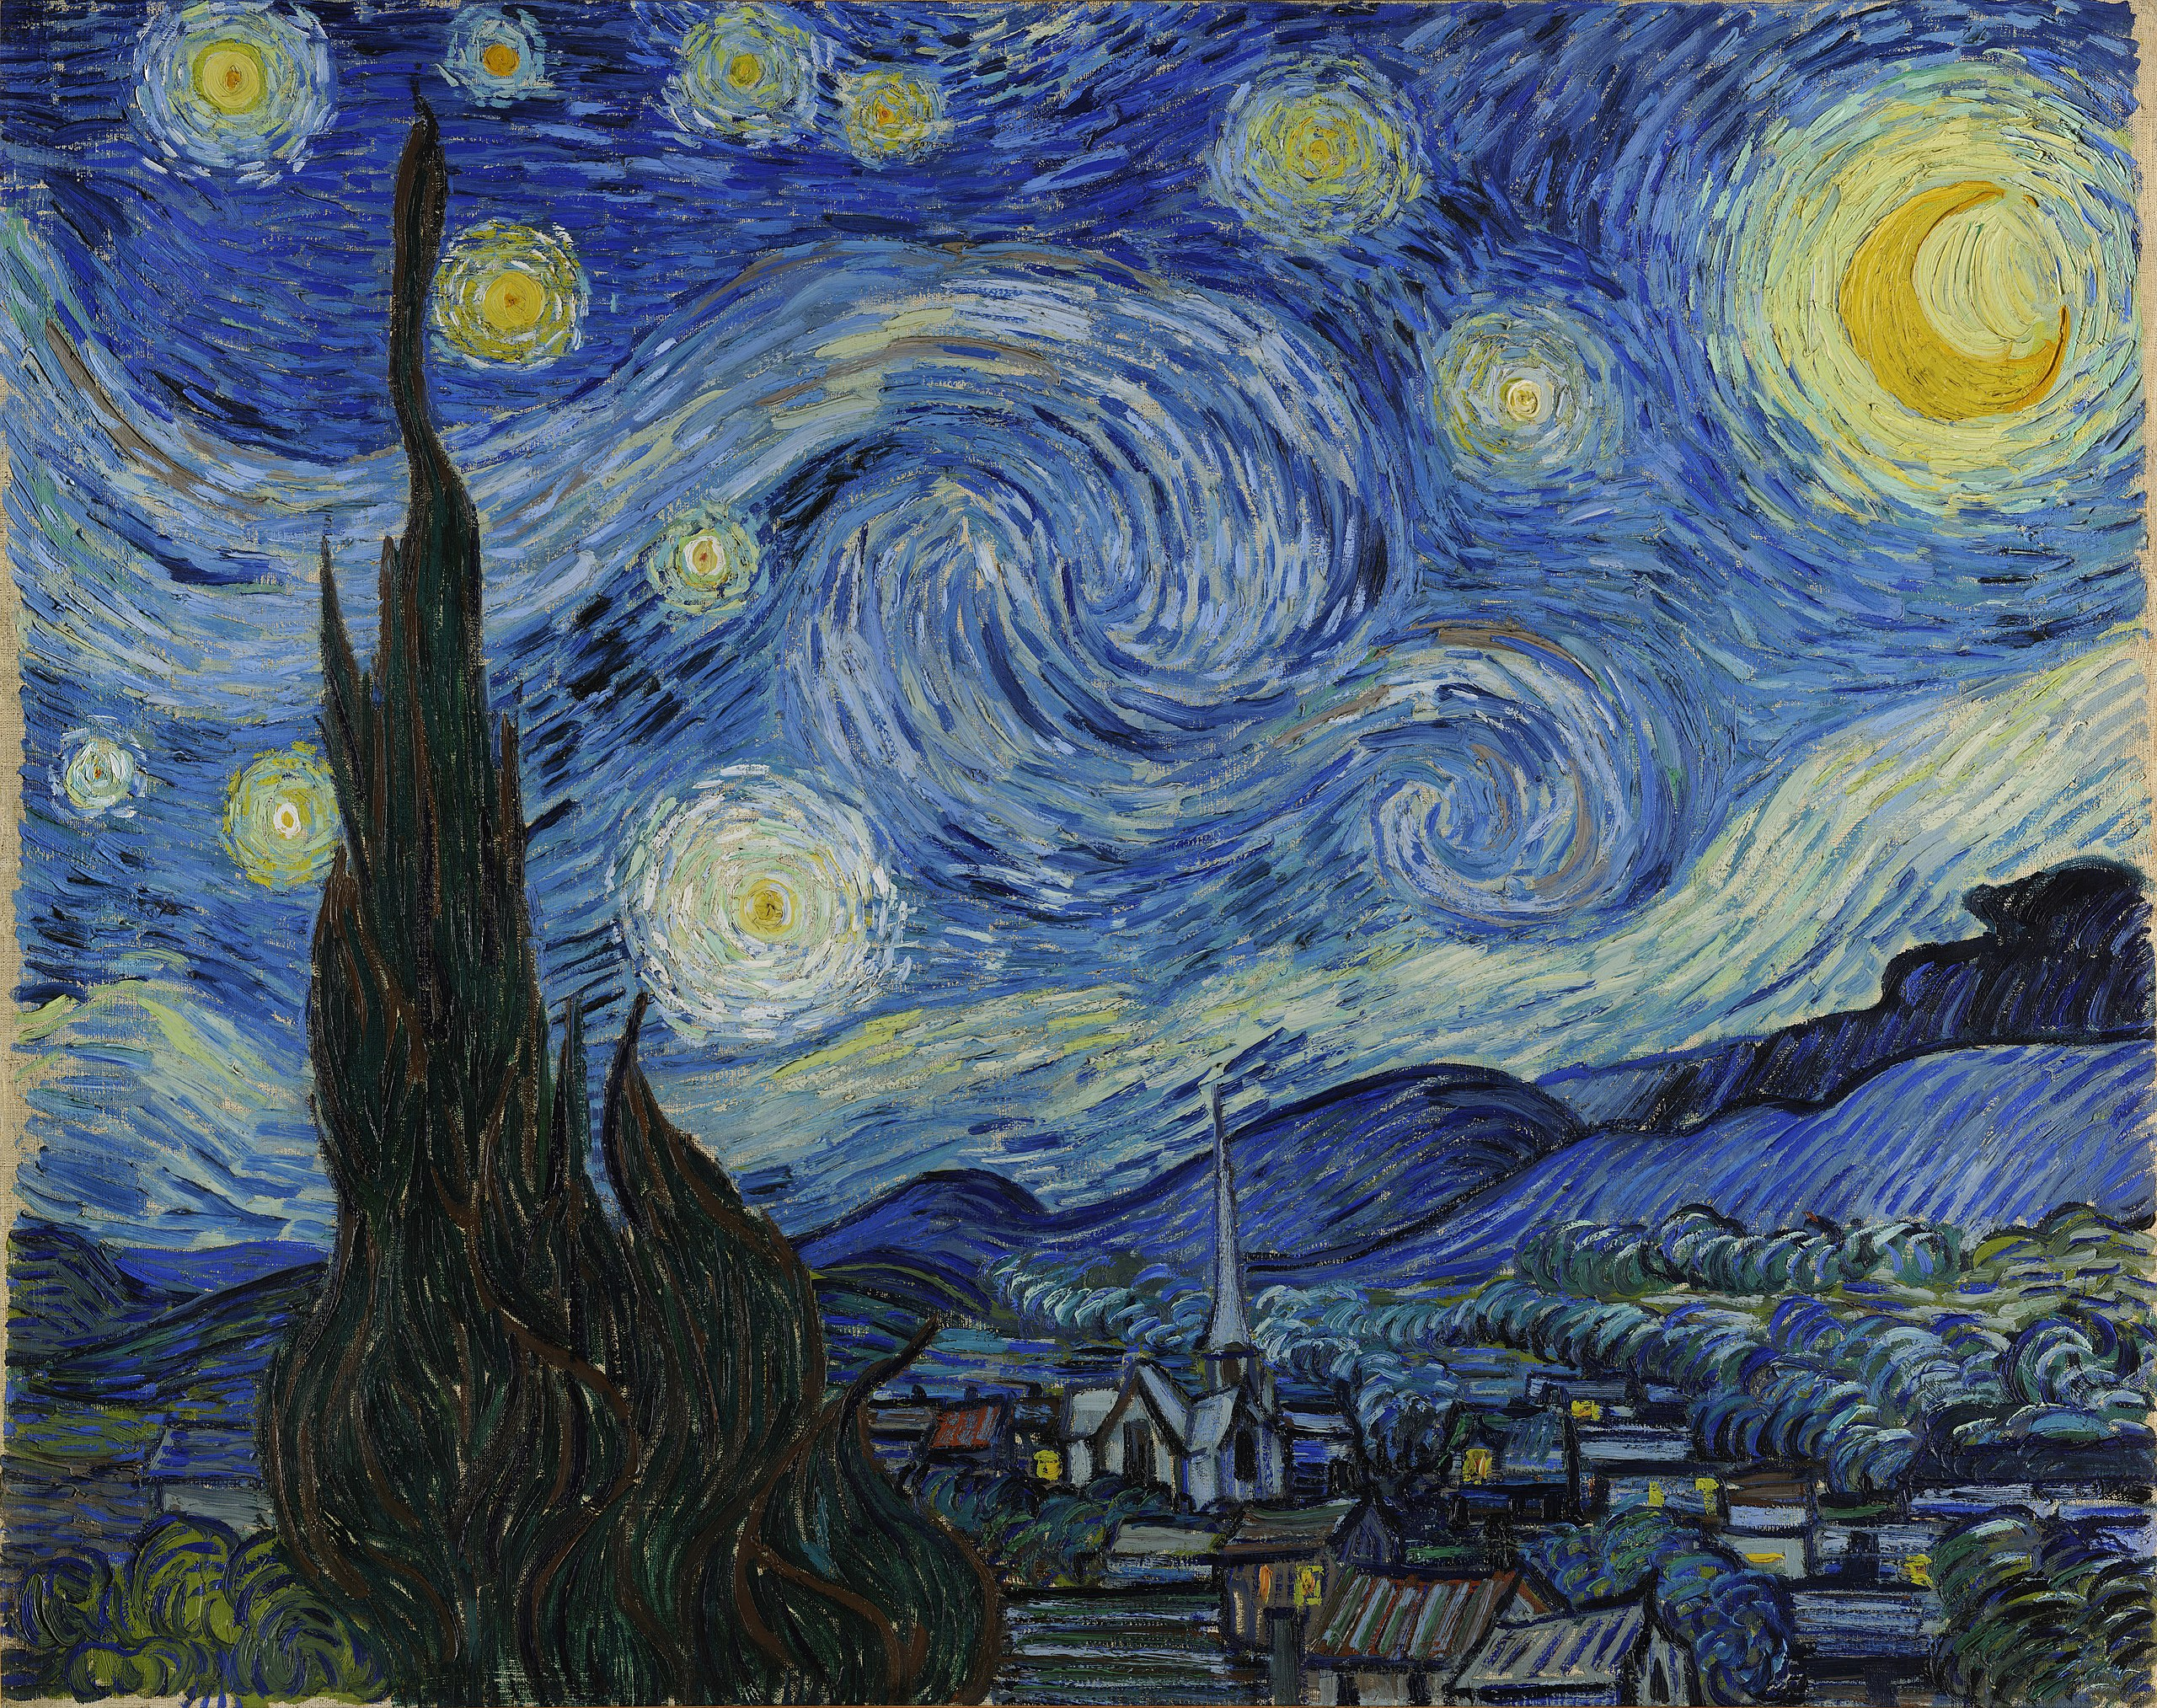
\includegraphics{figures/paintingexamples/starrynight}}
\caption{Like it or not, a continuous relation $[0,1] \rightarrow \blacksquare$: "The Starry Night", by Vincent van Gogh.}
\end{marginfigure}
\clearpage
\newpage
\section{Continuous Relations}

\newthought{To the best of my knowledge, the study of \textbf{TopRel} is a novel contribution. I venture two potential reasons.}

\newthought{First, it is because and not despite of the na\"{i}vity of the construction.} Usually, the relationship between \textbf{Rel} and \textbf{Set} is often understood in sophisticated general methods which are inappropriate in different ways. I have tried applying Kliesli machinery which generalises to "relationification" of arbitrary categories via appropriate analogs of the powerset monad to relate \textbf{Top} and \textbf{TopRel}, but it is not evident to me whether there is such a monad. The view of relations as spans of maps in the base category should work, since \textbf{Top} has pullbacks, but this makes calculation difficult and especially cumbersome when monoidal structure is involved. The na\"{i}ve approach I take is to observe that the preimages of functions are precisely relational converses when functions are viewed as relations, so the preimage-preserves-opens condition that defines continuous functions directly translates to the relational case.

\newthought{Second, the relational nature of \textbf{TopRel} means that the category has poor exactness properties.} Even if the sophisticated machinery mentioned in the first reason do manage to work, relational variants of \textbf{Top} are poor candidates for any kind of serious mathematics because they lack many limits and colimits. Since we take an entirely "monoidal" approach -- a relative newcomer in terms of mathematical technique -- we are able to find and make use of the rich structure of \textbf{TopRel} with a different toolkit.\\

In the end, we want to formalise doodles, so perhaps there is some virtue in proceeding by elementary means.

\marginnote{
\begin{rem}[Topological Space]
A \emph{topological space} is a pair $(X,\tau)$, where $X$ is a set, and $\tau \subset \mathcal{P}(X)$ are the \emph{open sets} of $X$, such that:
\begin{description}
    \item["nothing" and "everything" are open]  \[\varnothing,X \in \tau\]
    \item[Arbitrary unions of opens are open] \[\{ U_i : i \in I \} \subseteq \tau \Rightarrow \bigcup\limits_{i \in I} U_i \in \tau \]
    \item[Finite intersections of opens are open] $n \in \mathbb{N}$: \[U_1,\cdots, U_n \in \tau \Rightarrow \bigcap\limits_{1\cdots, i , \cdots n} U_i \in \tau\]
\end{description}
\end{rem}
}

\marginnote{
\begin{rem}[Relational Converse]
Recall that a relation $R: S \rightarrow T$ is a subset $R \subseteq S \times T$. \[R^\dag : T \rightarrow S := \{ (t,s) : (s,t) \in R \}\]
\end{rem}
}

\marginnote{
\begin{rem}[Continuous function]
A function between sets $f: X \rightarrow Y$ is a continuous function between topologies $f: (X,\tau) \rightarrow (Y,\sigma)$ if \[U \in \sigma \Rightarrow f^{-1}(U) \in \tau\] where $f^{-1}$ denotes the inverse image.
\end{rem}
}

Recall that functions are relations, and the inverse image used in the definition of continuous maps is equivalent to the relational converse when functions are viewed as relations. So we can na\"{i}vely extend the notion of continuous maps to continuous relations between topological spaces.

\begin{defn}[Continuous Relation]\label{defn:toprelation}
A continuous relation $R: (X,\tau) \rightarrow (Y,\sigma)$ is a relation $R: X \rightarrow Y$ such that \[U \in \sigma \Rightarrow R^{\dag}(U) \in \tau\] where $\dag$ denotes the relational converse.
\end{defn}

\begin{notation}
For shorthand, we denote the topology $(X,\tau)$ as $X^{\tau}$. As special cases, we denote the discrete topology on $X$ as $X^{\star}$, and the indiscrete topology $X^{\circ}$.
\end{notation}

The symmetric monoidal structure is that of product topologies on objects, and products of relations on morphisms.

\marginnote{
\begin{rem}[Product Topology]
We denote the product topology of $X^\tau$ and $Y^\sigma$ as $(X \times Y)^{(\tau \times \sigma)}$. $\tau \times \sigma$ is the topology on $X \times Y$ generated by the basis $\{t \times s : t \in \mathfrak{b}_\tau, s \in \mathfrak{b}_\sigma\}$, where $\mathfrak{b}_\tau$ and $\mathfrak{b}_\sigma$ are bases for $\tau$ and $\sigma$ respectively.
\end{rem}
}

\marginnote{
    \begin{rem}[Product of relations]
    For relations between sets $R: X \rightarrow Y, S: A \rightarrow B$, the product relation $R \times S: X \times A \rightarrow Y \times B$ is defined to be \[ \{ ((x,a),(y,b)) : (x,y) \in R, (a,b) \in S \} \]
    \end{rem}
}

\begin{fullwidth}

\section{\textbf{TopRel} diagrammatically}

\subsection{Relations that are always continuous}

\newthought{Here are five continuous relations for any $X^\tau$:}

\[\scalebox{0.75}{\tikzfig{bestiary/generators}}\]

\newthought{Copy and delete obey the following equalities:}

\[\scalebox{0.75}{\tikzfig{bestiary/basicrelations}}\]

\newthought{The copy map can also be used to distinguish the deterministic maps -- points and functions -- which we notate with an extra dot.}

\[\scalebox{0.75}{\tikzfig{structure/determinism}}\]

\newthought{Everything, delete, nothing-states and nothing-tests combine to give two numbers, one and zero.} There are extra expressions in grey squares above: they anticipate the tape-diagrams we will later use to graphically express another monoidal product of \textbf{TopRel}, the direct sum $\oplus$.

\[\scalebox{0.75}{\tikzfig{bestiary/scalarrelations}}\]

\newthought{Zero scalars turn entire diagrams into zero morphisms.} There is a zero-morphism for every input-output pair of objects in \textbf{TopRel}. 

\[\scalebox{0.75}{\tikzfig{bestiary/zerorelations}}\]

\end{fullwidth}
\clearpage
\newpage
\section{Populating space with shapes using sticky spiders}\label{sec:stickyspider}

%\begin{figure}\label{fig:spiderbicate}
%\scalebox{0.7}{\tikzfig{bestiary/spiderbicat}}
%\caption{The generators (in dashed boxes) and relations that make a spider. When the spider satisfies in addition the three inequalities b1-3, we call it a \textbf{relation-spider}.}
%\end{figure}

In this section, we seek to process-theoretically characterise disjoint collections of open sets of a space, so that we can play with doodles on the page as formal objects. It turns out that in \textbf{ContRel}, we can express them as idempotents that interact with spiders in a certain way.

\begin{example}[The copy-compare spiders of $\mathbf{Rel}$ are not always continuous]\label{ex:compnotspider}
The compare map for the Sierpi\'{n}ski space is not continuous, because the preimage of $\{0,1\}$ is $\{(0,0),(1,1)\}$, which is not open in the product space of $\mathcal{S}$ with itself.
\end{example}

\begin{rem}[copy-compare spiders of $\mathbf{Rel}$]
For a set $X$, the \emph{copy} map $X \rightarrow X \times X$ is defined:
\[\{(x,(x,x)) : x \in X \}\]
the \emph{compare} map $X \times X \rightarrow X$ is defined:
\[\{((x,x),x) : x \in X \}\]
These two maps are the (co)multiplications of special frobenius algebras. The (co)units are \emph{delete}:
\[\{(x,\star) : x \in X\}\]
and \emph{everything}:
\[\{(\star,x) : x \in X\}\]
\end{rem}

\newpage

\begin{myboxR}
\begin{proposition}\label{prop:copydiscrete}
The copy map is part of a special commutative frobenius algebra iff the topology is discrete.
\begin{proof}
Discrete topologies inherit the usual copy-compare spiders from \textbf{Rel}, so we have to show that when the copy map is part of a spider, the underlying wire must have a discrete topology. Suppose that some wire has a spider, and construct the following open set using an arbitrary point $p$:
\[\scalebox{0.5}{\tikzfig{structure/copyspiderproof/openpoint}}\]
It will suffice to show that this open set tests whether the input is the singleton $\{p\}$ -- when all singletons are open, the topology is discrete. As a lemma, we show that comparing distinct points $p \neq q$ yields the empty state.
\[\scalebox{0.5}{\tikzfig{structure/copyspiderproof/openpointproof}}\]
The (zero) implication follows since $p \neq q$ by assumption, so we know that deleting the comparison of $p$ and $q$ cannot be the unit scalar, and so must be the zero scalar, hence the comparison of $p$ and $q$ is the empty state. Now, the following case analysis shows that our open set only contains the point $p$.
\[\resizebox{0.75\textwidth}{!}{\tikzfig{structure/copyspiderproof/openpointcases}}\]
\end{proof}
\end{proposition}
\end{myboxR}

\begin{myboxB}
\begin{defn}[Sticky spiders]\label{defn:stickyspider}
A \textbf{sticky spider} (or just an $e$-spider, if we know that $e$ is a split idempotent), is a spider \emph{except} every identity wire on any side of an equation is replaced by the idempotent $e$.
\end{defn}

The desired graphical behaviour of a sticky spider is that one can still coalesce all connected spider-bodies together, but the 1-1 spider "sticks around" rather than disappearing as the identity. This is achieved by the following rules that cohere the idempotent $e$ with the (co)unit and (co)multiplications; they are the same as the usual rules for a special commutative frobenius algebra with two exceptions. First, where an identity wire appears in an equation, we replace it with an idempotent. Second, the monoid and comonoid components freely emit and absorb idempotents. By these rules, the usual proof [] for the normal form of spiders follows, except the idempotent becomes an explicit 1-1 spider, rather than the identity.
\[\resizebox{\textwidth}{!}{\tikzfig{structure/idemspider/stickyrelations}}\]
\end{myboxB}

\begin{myboxR}
\newthought{We can use split idempotents to transform copy-spiders from discrete topologies to sticky-spiders on other spaces.}
\begin{rem}[Split idempotents]
An \textbf{idempotent} in a category is a map $e: A \rightarrow A$ such that \[A \overset{e}{\rightarrow} A \overset{e}{\rightarrow} A = A \overset{e}{\rightarrow} A\]
A \textbf{split idempotent} is an idempotent $e: A \rightarrow A$ along with a \textbf{retract} $r: A \rightarrow B$ and a \textbf{section} $s: B \rightarrow A$ such that:
\[A \overset{e}{\rightarrow} A = A \overset{r}{\rightarrow} B \overset{s}{\rightarrow} A\]
\[B \overset{s}{\rightarrow} A \overset{r}{\rightarrow} B = B \overset{\mathop{id}}{\rightarrow} B\]
\end{rem}

We can graphically express the behaviour of a split idempotent $e$ as follows, where the semicircles for the section and retract $r,s$ form a visual pun. Recall that $X^\star$ denotes the discrete topology on the set $X$.

\[\scalebox{1}{\tikzfig{structure/idemspider/splitidem}}\]
\end{myboxR}

\begin{myboxB}
\begin{construction}[Sticky spiders from split idempotents]\label{cons:stickyfromsplit}
Given an idempotent $e: Y^\sigma \rightarrow Y^\sigma$ that splits through a discrete topology $X^\star$, we construct a new (co)multiplication as follows:
\[\scalebox{1}{\tikzfig{structure/idemspider/idemspiderv2}}\]
\end{construction}
\end{myboxB}

\begin{myboxR}
\begin{proposition}[Every idempotent that splits through a discrete topology gives a sticky spider]\label{prop:splitmeanssticky} The following is a sticky spider:
\[\scalebox{1}{\tikzfig{structure/idemspider/espiderstatement}}\]
\end{proposition}
We can check that Construction \ref{cons:stickyfromsplit} satisfies the frobenius rules as follows. We only present one equality; the rest follow the same idea.
\[\scalebox{1}{\tikzfig{structure/idemspider/espiderproofv2}}\]
\end{myboxR}
\begin{myboxR}
To verify the sticky spider rules, we first observe that since $X^\star \overset{s}{\rightarrow} Y^\sigma \overset{r}{\rightarrow} X^\star = X^\star \overset{\mathop{id}}{\rightarrow} X^\star$, $r$ must have all of $X^\star$ in its image, and $s$ must have all of $X^\star$ in its preimage, so we have the following:
\[\scalebox{1}{\tikzfig{structure/idemspider/splitonto}}\]
Now we show that e-unitality holds:
\[\scalebox{1}{\tikzfig{structure/idemspider/espiderproof2}}\]
The proofs of e-counitality, and e-speciality follow similarly.
\end{myboxR}

\begin{myboxB}
\newthought{We can prove a partial converse of Proposition \ref{prop:splitmeanssticky}:} we can identify two diagrammatic equations that tell us precisely when a sticky spider has an idempotent that splits though some discrete topology.
\begin{theorem}\label{thm:stickygraphical}
A sticky spider has an idempotent that splits through a discrete topology if and only if in addition to the sticky spider equalities, the following relations are also satisfied.
\[\scalebox{1}{\tikzfig{idemproof/unit-everything}} \quad\quad\quad\quad\quad\quad\quad\quad \scalebox{1}{\tikzfig{idemproof/comult-copy}}\]
\end{theorem}
The proof is involved, so here is a map of lemmas and propositions.
\[\resizebox{0.8\textwidth}{!}{\tikzfig{idemproof/claimmap2}}\]
\end{myboxB}

\begin{myboxR}
\begin{proposition}[comult/copy implies counit/delete]\label{prop:counitdelete}
\[\scalebox{1}{\tikzfig{idemproof/ecopy2delclaim}}\]
\begin{proof}
\[\scalebox{1}{\tikzfig{idemproof/ecopy2del}}\]
\end{proof}
\end{proposition}
\end{myboxR}

\begin{myboxB}
\begin{lemma}[All-or-Nothing]\label{lem:allornothing}
Consider the set $e(\{x\})$ obtained by applying the idempotent $e$ to a singleton $\{x\}$, and take an arbitrary element $y \in e(x)$ of this set. Then $e(\{y\}) = \varnothing$ or $e(\{x\}) = e(\{y\})$. Diagrammatically: \[\scalebox{0.75}{\tikzfig{idemproof/allornothingclaim}}\]
\end{lemma}
\[\scalebox{0.75}{\tikzfig{idemproof/allornothing2a}}\]
\end{myboxB}
\begin{myboxB}
\[\scalebox{0.75}{\tikzfig{idemproof/allornothing2b}}\]
\end{myboxB}

\begin{myboxR}
\begin{proposition}[$e$ of any point is $e$-copiable]\label{prop:epointcopy}
\[\scalebox{0.75}{\tikzfig{idemproof/pointidemcopiable}}\]
\begin{proof}
\[\scalebox{0.75}{\tikzfig{idemproof/pointidemcopiableproof}}\]
\end{proof}
\end{proposition}
\end{myboxR}

\begin{myboxB}
\begin{proposition}[The unit is the union of all $e$-copiables]\label{prop:copiablebasis}
\[\scalebox{0.8}{\tikzfig{idemproof/copiablebasisclaim}}\]
\begin{proof}
\[\scalebox{0.8}{\tikzfig{idemproof/copiablebasis}}\]
\end{proof}
\end{proposition}
\end{myboxB}

\begin{myboxR}
\begin{proposition}[$e$-copiable decomposition of $e$]\label{prop:decompidem}
\[\scalebox{1}{\tikzfig{idemproof/decompidemclaim}}\]
\begin{proof}
\[\scalebox{1}{\tikzfig{idemproof/decompidem}}\]
\end{proof}
\end{proposition}
\end{myboxR}

\begin{myboxB}
\begin{proposition}[$e$-copiable decomposition of counit]\label{prop:decompcounit}
\[\scalebox{1}{\tikzfig{idemproof/decompcounitclaim}}\]
\begin{proof}
\[\scalebox{1}{\tikzfig{idemproof/decompcounit}}\]
\end{proof}
\end{proposition}
\end{myboxB}

\begin{myboxR}
\newthought{The $e$-copiable states really do behave like an orthonormal basis, as the following Lemmas show.}
\begin{lemma}[$e$-copiables are orthogonal under multiplication]\label{lem:match}
\[\scalebox{0.75}{\tikzfig{idemproof/matchclaim}}\]
\begin{proof}
\[\scalebox{0.75}{\tikzfig{idemproof/match}}\]
\end{proof}
\end{lemma}
\end{myboxR}

\begin{myboxB}
\begin{convention}[Shorthand for the open set associated with an $e$-copiable]
We introduce the following diagrammatic shorthand.
\[\scalebox{1}{\tikzfig{idemproof/openshorthand}}\]
Including the coloured dot is justified, because these open sets are co-copiable with respect to the multiplication of the sticky spider.
\[\scalebox{1}{\tikzfig{idemproof/shorthandjustification}}\]
\end{convention}
\end{myboxB}

\begin{myboxR}
\begin{lemma}[Co-match]\label{lem:comatch}
\[\scalebox{1}{\tikzfig{idemproof/comatchclaim}}\]
\begin{proof}
\[\scalebox{0.9}{\tikzfig{idemproof/comatch}}\]
The claim then follows by applying Lemma \ref{lem:match} to the final diagram.
\end{proof}
\end{lemma}
\end{myboxR}

\begin{myboxB}
\begin{lemma}[e-copiables are e-fixpoints]\label{lem:ecopyfixpoint}
\[\scalebox{1}{\tikzfig{idemproof/dotcopyableclaim}}\]
\begin{proof}
\[\scalebox{1}{\tikzfig{idemproof/dotcopyable}}\]
Observe that the final equation of the proof also holds when the initial e-copiable is the empty set.
\end{proof}
\end{lemma}
\end{myboxB}

\begin{myboxR}
\begin{lemma}[$e$-copiables are normal]\label{lem:ecopynormal}
\[\scalebox{1}{\tikzfig{idemproof/copynormalclaim}}\]
\begin{proof}
\[\scalebox{1}{\tikzfig{idemproof/copynormal}}\]
\end{proof}
\end{lemma}
\end{myboxR}

\begin{myboxB}
\begin{proposition}[$e$-copiable decomposition of multiplication]\label{prop:decompmult}
\[\scalebox{1}{\tikzfig{idemproof/decompmultclaim}}\]
\begin{proof}
\[\scalebox{1}{\tikzfig{idemproof/decompmult}}\]
\end{proof}
\end{proposition}
\end{myboxB}

\begin{myboxR}
\begin{proposition}[$e$-copiable decomposition of comultiplication]\label{prop:decompcomult}
\[\scalebox{1}{\tikzfig{idemproof/decompcomultclaim}}\]
\begin{proof}
\[\scalebox{1}{\tikzfig{idemproof/decompcomult}}\]
\end{proof}
\end{proposition}
\end{myboxR}

\begin{myboxB}
\newthought{Now we can prove Theorem \ref{thm:stickygraphical}.}
First a reminder of the claim; we want to show that when given a sticky spider, the following relations hold if and only if the idempotent splits through a discrete topology.
\[\scalebox{0.8}{\tikzfig{idemproof/unit-everything}} \quad\quad\quad\quad\quad\quad\quad\quad \scalebox{0.8}{\tikzfig{idemproof/comult-copy}}\]
The crucial observation is that the $e$-copiable decomposition of the idempotent given by Proposition \ref{prop:decompidem} is equivalent to a split idempotent though the set of $e$-copiables equipped with discrete topology.
\[\scalebox{0.8}{\tikzfig{idemproof/finalproof}}\]
By copiable basis Proposition \ref{prop:copiablebasis} and the decompositions Propositions \ref{prop:decompcounit}, \ref{prop:decompmult}, \ref{prop:decompcomult}, we obtain the only-if direction.
\[\scalebox{0.8}{\tikzfig{idemproof/finalproof2}}\]
\end{myboxB}
\begin{myboxB}
The if direction is an easy check. For the unit/everything relation, we have:
\[\scalebox{0.8}{\tikzfig{idemproof/finalproof3}}\]
For the counit/delete relation, we observe that for any split idempotent, the retract must be a partial function. To see this, suppose the split idempotent $e = r;s$ is on $(X,\tau)$ and the discrete topology is $Y^\star$. Seeking contradiction, if the retract is not a partial function, then there is some point $x \in X$ such that $x \in e(x)$, and the image $I := r(x) \subseteq Y$ contains more than one point, which we denote and discriminate $a,b \in r(x) \subseteq Y$ and $a \neq b$. Because the composite $s;r = 1_Y$ of the section and retract must recover the identity on $Y^\star$, the section $s$ must be total -- i.e. the image $s(X) = Y$. So $x \in s(a) \cap s(b)$. Now we have that $(a,x),(b,x) \in s$, and $(x,a),(x,b) \in r$, therefore $(a,b),(b,a) \in s;r$, which by $a \neq b$ contradicts that $s;r$ is the identity relation $1_Y$.
\[\scalebox{0.8}{\tikzfig{idemproof/finalproof4}}\]
\end{myboxB}

\begin{myboxR}
\begin{defn}[Labels, shapes, cores, halos]
Recall by Proposition \ref{prop:decompidem} that we can express the idempotent as a union of continuous relations formed of a state and test, for some indexing set of \emph{labels} $\mathcal{L}$.
\[\tikzfig{topology/shape1}\]
A \emph{shape} is a component of this union corresponding to some arbitary $l \in L$. So we refer to a sticky spider as a labelled collection of shapes. The state of a shape is the \emph{halo} of the shape. The halos are precisely the copiables of the sticky spider. The test of a shape is the \emph{core}. The cores are precisely the cocopiables of the sticky spider.
\[\tikzfig{topology/shape2}\]
\end{defn}
\end{myboxR}

\begin{myboxB}
\begin{proposition}[Core exclusion: Distinct cores cannot overlap]\label{prop:core-core-exclusion}
\begin{proof}
A direct consequence of Lemma \ref{lem:comatch}.
\end{proof}
\end{proposition}
\end{myboxB}

\begin{myboxR}
\begin{proposition}[Core-halo exclusion: Each core only overlaps with its corresponding halo]\label{prop:core-halo-exclusion}
\begin{proof}
Seeking contradiction, if a core overlapped with multiple halos, Lemma \ref{lem:ecopyfixpoint} would be violated.
\end{proof}
\end{proposition}
\end{myboxR}

\begin{myboxB}
\begin{proposition}[Halo non-exclusion: halos may overlap]
\begin{proof}
By example:
\[\tikzfig{topology/halooverlap}\]
The two shapes are colour coded cyan and magenta. The halos are two triangles which overlap at a yellow region, and partially overlap with their blobby cores. The cores are outlined in dotted blue and orange respectively. Observe that cores and halos do not have to be simply connected; in this example the core of the magenta shape has two connected components. Viewing these sticky spiders as a process, any shape that overlaps with the magenta core will be deleted and replaced by the magenta triangle, and similarly with the cyan cores and triangle. Any shape that overlaps with both the magenta and cyan cores will be deleted and replaced by the union of the triangles. Any shape that overlaps with neither core will be deleted and not replaced.
\end{proof}
\end{proposition}
\end{myboxB}

\begin{myboxR}
\begin{corollary}[Only opens please]
A sticky spider corresponds to a set-indexed disjoint collection of open sets when, in addition to the equations of Theorem \ref{thm:stickygraphical}, it satisfies one more, depicted below on the left.
\[\scalebox{1}{\tikzfig{idemproof/opensonly}}\]
Observe that the right hand equation above is precisely what we want expressed in diagrams: that every halo matches its core. For the forward direction, we have:
\[\scalebox{1}{\tikzfig{idemproof/opensonly3}}\]
\end{corollary}
\end{myboxR}

\begin{myboxR}
For the backward direction, we rely on the fact that cores are non-empty (or else we would fail to satisfy the identity equation of the split idempotent) to eliminate the floating scalars.
\[\scalebox{1}{\tikzfig{idemproof/opensonly2}}\]
By Proposition \ref{prop:core-core-exclusion}, we have disjointness.\\

So, without loss of generality, we may treat any collection of disjoint open shapes on a page as a sticky spider.
\end{myboxR}

\clearpage

\clearpage
\newpage
\chapter{Sketches in iconic semantics}\label{chapter:contrel}
How to reason formally with and about pictorial iconic representations as a semantics of natural language.
\clearpage
\newpage
\section{Preliminary concepts for the sketches}

This section should be read as a smooth transition from the contents of the previous chapter towards sketches that gradually trade off rigour for expressivity, while ideally being descriptive enough that the reader trusts that the necessary details can be worked out.

\subsection{Open sets: concepts}

Apart from enabling us to paint pictures with words, \textbf{ContRel} is worth the trouble because the opens of topological spaces crudely model how we talk about concepts, and the points of a topological space crudely model instances of concepts. We consider these open-set tests to correspond to "concepts", such as redness or quickness of motion. Figure \ref{fig:pointing} generalises to a sketch argument that insofar as we conceive of concepts in (possibly abstractly) spatial terms, the meanings of words are modellable as shared strategies for spatial deixis; absolute precision is communicatively impossible, and the next best thing mathematically requires topology.

\begin{figure}[h!]\label{fig:pointing}
\[\resizebox{\textwidth}{!}{\tikzfig{topology/pointingfinger}}\]
\caption{Points in space are a useful mathematical fiction. Suppose we have a point on a unit interval. Consider how we might tell someone else about where this point is. We could point at it with a pudgy appendage, or the tip of a pencil, or give some finite decimal approximation. But in each case we are only speaking of a vicinity, a neighbourhood, an \emph{open set in the borel basis of the reals} that contains the point. Identifying a true point on a real line requires an infinite intersection of open balls of decreasing radius; an infinite process of pointing again and again, which nobody has the time to do. In the same way, most language outside of mathematics is only capable of offering successively finer, finite approximations.}
\end{figure}

Maybe this explains the asymmetry of why tests are open sets, but why are states allowed to be arbitrary subsets? One could argue that states in this model represent what is conceived or perceived. Suppose we have an analog photograph whether in hand or in mind, and we want to remark on a particular shade of red in some uniform patch of the photograph. As in the case of pointing out a point on the real interval, we have successively finer approximations with a vocabulary of concepts: "red", "burgundy", "hex code \#800021"... but never the point in colourspace itself. If someone takes our linguistic description of the colour and tries to reproduce it, they will be off in a manner that we can in principle detect, cognize, and correct: "make it a little darker" or "add a little blue to it". That is to say, there are in principle differences in mind that we cannot distinguish linguistically in a finite manner; we would have to continue the process of "even darker" and "add a bit less blue than last time" forever. All this is just the mathematical accommodation of a common observation: sometimes you cannot do an experience justice with words, and you eventually give up with "I guess you just had to be there". Yet the experience is there and we can perform linguistic operations on it.

\clearpage
\subsection{Copy: stative verbs and adjectives}

\emph{Stative} verbs are those that posit an unchanging state of affairs, such as \texttt{Bob \underline{likes} drinking}. Insofar as stative verbs are restrictions of all possible configurations to a permissible subset, they are conceptually similar to adjectives, such as \texttt{\underline{red} car}, which restricts permissible representations in colourspace. When we interpret concepts as open-set tests, \textbf{ContRel} conspires in our favour by giving us free copy maps on every wire. This allows us to define a family of processes that behave like stative restrictions of possibilities.

\[\resizebox{\textwidth}{!}{\tikzfig{topology/copygatecommute}}\]
The desirable property we obtain is that in the absence of \emph{dynamic} verbs that posit a change in the state of affairs, stative constructions commute in text: if I'm just telling you static properties of the way things are, it doesn't matter in what order I tell you the facts because restrictions commute. Recall that gates of the following form are intersections with respect to open sets, and they commute. These intersections model conjunctive specifications of properties.

\begin{example}[Containment and insideness]
\[\resizebox{0.8\textwidth}{!}{\tikzfig{topology/oxfordex}}\]
Consider the configuration space of a sticky spider on the unit square with three labelled shapes, which has 6 connected components, depicted. \texttt{Oxford contains Catz.} restricts away configurations where \texttt{Catz} is not enclosed in \texttt{Oxford}. Adding on \texttt{England contains Oxford.} further restricts away incongruent configurations, leaving us only with a single connected component, which contains all spatial configurations that satisfy the text. A similar story holds for abstract conceptual spaces, in which \texttt{fast red car}, \texttt{fast car that is red}, \texttt{car is (red and fast)} all mean the same thing.
\end{example}


\subsection{Coclosure: adverbs and adpositions}

\begin{figure}[h!]
\[\scalebox{0.9}{\tikzfig{topology/adverbex1}}\]
\caption{
Recall that \textbf{ContRel} is coclosed (Proposition \ref{prop:coclosure}), which means that every dynamic verb may be expressed as the composite of a coevaluator and an open set on the space of homotopies. For instance, \texttt{move} is an intransitive dynamic verb, which corresponds to a concept in the space of all movements.
}
\end{figure}

\begin{figure}[h!]
\[\scalebox{0.9}{\tikzfig{topology/adverbex2}}\]
\caption{
Adverb-boxes may be modelled as static restrictions in movement-space. For instance, \texttt{straight} may restrict movements to just those that satisfy some notion of path-length minimality: e.g., given a metric in movement-space on path-lengths, we may construct an open ball (Definition \ref{def:openball}) around the geodesic to model the adverb \texttt{straight}.
}
\end{figure}

\begin{figure}[h!]
\[\scalebox{0.9}{\tikzfig{topology/adverbex3}}\]
\caption{
Similarly, adposition-boxes may be modelled as static restrictions on the product of the spaces of nouns and verbs. For instance, \texttt{towards} may be modelled as an open set that pairs potential positions of the thing-being-moved-towards with movements in movement-space that indeed move towards the target.
}
\end{figure}

\subsection{Using sticky spiders as location-tests}

\begin{myboxB}
\begin{example}[Where is a piece on a chessboard?]\label{ex:chessboard}
How is it that we quotient away the continuous structure of positions on a chessboard to locate pieces among a discrete set of squares? Evidently shifting a piece a little off the centre of a square doesn't change the state of the game, and this resistance to small perturbations suggests that a topological model is appropriate. We construct two spiders, one for pieces, and one for places on the chessboard. For the spider that represents the position of pieces, we open balls of some radius $r$, and we consider the places spider to consist of square halos (which tile the chessboard), containing a core inset by the same radius $r$; in this way, any piece can only overlap at most one square. As a technical aside, to keep the core of the tiles open, we can choose an arbitrarily sharp curvature $\epsilon$ at the corners.
\[\scalebox{0.70}{\tikzfig{topology/chessboard}}\]
Now we observe that the calculation of positions corresponds to composing sticky spiders. We take the initial state to be the sticky spider that assigns a ball of radius $r$ on the board for each piece. We can then obtain the set of positions of each piece by composing with the places spider. The composite (pieces;places)
will send the king to a2, the bishop to b4, and the knight to d1, i.e. $\bra{K} \mapsto \bra{a2}$, $\bra{B} \mapsto \bra{b4}$ and $\bra{N} \mapsto \bra{d1}$. In other words, we have obtained a process that models how we pass from continuous states-of-affairs on a physical chessboard to an abstract and discrete game-state.
\[\resizebox{0.70\textwidth}{!}{\tikzfig{topology/chessboard2a}}\]
\end{example}
\end{myboxB}

\clearpage

\subsection{The unit interval}
\marginnote{\textcolor{blue}{Postscript: If you're already happy that in principle we may either start with nicer spaces or otherwise restrict ourselves to contractible opens, then you may skip the next two subsections and just glance at how relational homotopies differ from regular homotopies, and look briefly at the definition of a nice spider at the end. The relevant conceptual takeaway for the couple of sketches is that one may recover the usual topological notions such as simple connectivity, metrics and their open balls, and contractibility, from which one can in principle construct models of linguistic topological relations such as \texttt{touching}, \texttt{enclosure}, and so on. The submitted version of this thesis had detailed constructions of these linguistic topological relations "from scratch" but I've cut them, so only the next two sketches remain as artifacts to suggest that "low-level" hacking in \textbf{ContRel} is doable. I've opted to remove sketches of linguistic topological relations because (1) they took up too much space for too little gain (2) they still admitted counterexamples, and (3) it seems plausible that any analysis of linguistic topological primitives in mathematical terms will admit counterexamples, because I suspect they have the status of semantic primes \citep{wierzbicka_semantics_1996}, which are characterised by their universality across languages and their unanalysability in simpler terms.}} To begin modelling more complex concepts, we first need to extend our topological tools. Throughout, we now consider string-diagrams to be expressions that may be quantified over, and we allow ourselves additional niceties like endocombinators. Ultimately we would like to get at the unit interval so we can do homotopies to move shapes around, which we plan to arrive at by first expressing the reals, and then adding in endpoints. However, there are many spaces homeomorphic to the real line. How do we know when we have one of them? The following theorem provides an answer:
\begin{theorem}[\citep{friedman_fom_2005}]\label{thm:Friedman}
Let $\big((X,\tau), < \big)$ be a topological space with a total order. If there exists a continuous map $f: X \times X \rightarrow X$ such that $\forall a,b_{\in X} : a < f(a,b) < b$, then $X$ is homeomorphic to $\mathbb{R}$.
\end{theorem}
\begin{defn}[Less than]\label{defn:lessthan}
We define a total ordering relation $<$ as an open set on $X \times X$ that obeys the usual axiomatic rules:
\[\resizebox{\textwidth}{!}{\tikzfig{topology/lessthan}}\]
\[\scalebox{0.65}{\tikzfig{topology/lessthantotal}}\]
\end{defn}
\begin{defn}[Friedman's function]\label{defn:friedfunct}
Just as a wire in \textbf{ContRel} has the discrete topology if it possesses spider structure (Proposition \ref{prop:copydiscrete}), a wire is homeomorphic to the real line by Theorem \ref{thm:Friedman} if it possesses an open that behaves as Definition \ref{defn:lessthan}, and a map that satisfies:
\[\resizebox{\textwidth}{!}{\tikzfig{topology/betweenfunct}}\]
\end{defn}

Let's say that the unit interval is like the real line extended with endpoints. One way to define this that aligns with the usual presentation of the reals in analysis is to provide the ability to take suprema and infima of subsets, which are functions that map subsets to points. This kind of function is subsumed by a kind of structure on a category called an endocombinator.

\begin{defn}[Endocombinator]
An \emph{endocombinator} on a category $\mathcal{C}$ is a family of functions on homsets typed $\mathcal{C}(X,Y) \rightarrow \mathcal{C}(X,Y)$, for all objects $X,Y$.
\end{defn}

\begin{defn}[Upper and lower bounds via endocombinators]\label{defn:bounds}
Upper bounds are endocombinators that send states to points, which we depict as a little gray lassoed region around the state of interest. Recall that points are states with a little decorating copy-dot as they are copiable. The following equational condition quantified over all states characterises an "upper bound" endocombinator that returns an upper bound for any subset of a totally ordered space: in prose, such subsets are all less than their upper bound.
\[\tikzfig{topology/upperbound}\]
\end{defn}
We can add in further equations governing the upper bound endocombinator to turn it into a supremum, or least-upper-bound.
\begin{defn}[Suprema]\label{defn:sup}
An upper bound endocombinator is the supremum when the following additional condition (with caveats, see sidenote\marginnote{Unless $y$ already contains $\text{sup}(x)$, so the consequent of the implication needs a disjunctive case where $\text{sup}(x) \cup y|_{\text{sup}(x)<} = y$. The reason we cannot use $\leq$ as an open (even though it would make this definition easier) is that it would imply the equality relation $=$ is an open, which would imply that the underlying space has the discrete topology, trivialising everything.}) holds: for all subsets $y$ whose elements are all greater than those of a subset $x$, the supremum of $x$ is less than all elements of $y$.
\[\tikzfig{topology/sup}\]
\end{defn}
Now the lower endpoint is expressible as the supremum of the empty set, and the upper endpoint is the supremum of the whole set.
\begin{defn}[Endpoints]\label{defn:endpoints}
The lower endpoint is the supremum of the empty state, and the upper the supremum of everything. 
\[\tikzfig{topology/endpoints}\]
\end{defn}

\begin{defn}[The unit interval]
In \textbf{ContRel}, an object equipped with a less-than relation (Definition \ref{defn:lessthan}), Friedman's function (Definition \ref{defn:friedfunct}), and suprema (Definitions \ref{defn:bounds} and \ref{defn:sup}) is homeomorphic to the unit interval\marginnote{Conceptually, we are embedding the real line into a new space with two extra points, and then defining an extension of the less-than relation in terms of suprema to accommodate those points to characterise them as endpoints.}. Going forward, we will denote the unit interval using a thick dotted wire.
\end{defn}

\clearpage

\begin{example}[Simple connectivity]\label{def:simpconn}
Recall that we notate points and functions with the same small black dot for copying and deleting, as points are precisely the states that are copy-delete cohomomorphisms. In prose, simple connectivity states that for any pair of points that are within the open $V$, there exists some continuous function from the unit interval into the space that starts at one of the points and ends at the other. The left pair of conditions state that the points $\textcolor{blue}{x}$ and $\textcolor{red}{y}$ are within $V$. The right triple of conditions require the the image of the homotopy $\textcolor{orange}{f}$ is contained in $V$, and that its endpoints are $\textcolor{blue}{x}$ and $\textcolor{red}{y}$.
\[\resizebox{\textwidth}{!}{\tikzfig{topology/simplyconnected}}\]
Simple connectivity is a useful enough concept that we will notate simply connected open sets as follows, where the hole is a reminder that simply connected spaces might still have holes in them.
\[\tikzfig{topology/simpconnotation}\]
\end{example}

\clearpage

\subsection{Metric structure}

\begin{defn}[Addition]\label{def:addition}
In order to define metrics, we must have additive structure, which we encode as an additive monoid that is a function. All we need to know is that the lower endpoint of the unit interval stands in for "zero distance" -- as the unit of the monoid -- and that adding positive distances together will deterministically give you a larger positive distance.
\[\resizebox{\textwidth}{!}{\tikzfig{topology/addition}}\]
\end{defn}

\begin{defn}[Metric]\label{def:metric}
A metric on a space is a continuous map $X \rightarrow \mathbb{R}^+$ to the positive reals that satisfies the following axioms. We depict metrics as trapezoids.
\[\resizebox{\textwidth}{!}{\tikzfig{topology/metric}}\]
\end{defn}

\clearpage

\begin{example}[Open balls]\label{def:openball}
Once we have metrics, we can define the usual topological notion of open balls. With respect to a metric, an $\varepsilon$-open ball at $\textcolor{blue}{x}$ is the open set (effect) of all points that are $\varepsilon$-close to $\textcolor{blue}{x}$ by the chosen metric.
\[\tikzfig{topology/openball2}\]
Open balls will come in handy later, and a side-effect which we note but do not explore is that open balls form a basis for any metric space, so in the future whenever we construct spaces that come with natural metrics, we can speak of their topology without any further work.
\end{example}

\clearpage

\subsection{Relational homotopy}

\begin{defn}[Homotopy in \textbf{Top}]
where $f$ and $g$ are continuous maps $A \rightarrow B$, a \emph{homotopy} $\eta : f \Rightarrow g$ is a continuous function $\eta : [0,1] \times A \rightarrow B$ such that $\eta(0,-) = f(-)$ and $\eta(1,-) = g(1,-)$.
\end{defn}

In other words, a homotopy is like a short film where at the beginning there is an $f$, which continuously deforms to end the film being a $g$. Directly replacing "function" with "relation" in the above definition does not quite do what we want, because we would be able to define the following "homotopy" between open sets.

\[\tikzfig{topology/homotopyctrex1}\]

What is happening in the above film is that we have our starting open set in blue, which stays constant for a while. Then suddenly the ending open set in red appears, and then the blue open disappears, and we are left with our ending; while \emph{technically} there was no discontinuous jump, this isn't the notion of sliding we want. The exemplified issue is that we can patch together (by union of continuous relations) vignettes of continuous relations that are not individually total on $[0,1]$. We can patch this issue in by asking for homotopies in \textbf{ContRel} to satisfy the additional condition that they are expressible as a union of regular homotopies.

\clearpage

\marginnote{Observe that the second condition asking for decomposition in terms of partial functions (of which total functions are a special case) comes for free by Proposition \ref{prop:hombasis}, as the partial functions form a topological basis. the constraint of the definition is provided by the first condition, which is a stronger condition than just asking that the original continuous relation be total on $I$. Definition \ref{defn:homotopy} is "natural" in light of Proposition \ref{prop:hombasis}, that the partial continuous functions $A \rightarrow B$ form a basis for $\mathbf{ContRel}(A,B)$: we are just asking that homotopies between partial continuous functions -- which can be viewed as regular homotopies with domain restricted to the subspace topology induced by an open set -- form a basis for homotopies between continuous relations.}
\begin{defn}[Relational Homotopy]\label{defn:homotopy}
\[\resizebox{\textwidth}{!}{\tikzfig{topology/homotopy}}\]
\end{defn}

\clearpage

\begin{example}[Contractibility]\label{defn:contractible}
With homotopies in hand, we can define a stronger notion of connected shapes with no holes, which are usually called \emph{contractible}. The reason for the terminology reflects the method by which we can guarantee a shape in flatland has no holes: when any loop in the shape is \emph{contractible} to a point.
\[\resizebox{\textwidth}{!}{\tikzfig{topology/contractible}}\]
Contractible open sets are worth their own notation; a solid black effect, this time with no hole.
\[\tikzfig{topology/contractnotation}\]
\end{example}

\subsection{Nice spiders}

Let's assume for simplicity that henceforth, unless otherwise specified, we only deal with \emph{nice} sticky-spiders where cores and halos agree and are both contractible opens; i.e. the spider can be expressed as a finite union of open solid blobs as effects followed by the same open solid blob as a state.

\begin{defn}[Nice sticky-spiders]
A sticky-spider is \emph{nice} if it is equal to a union of contractible open effects followed by the same contractible open expressed as a state.
\[\tikzfig{topology/nicespider}\]
\end{defn}
\clearpage
\newpage
\section{Composition of dynamic verbs via temporal anaphora}
\marginnote{\textcolor{blue}{Postscript: These sketches are mostly a restructuring of content that otherwise dangled from the previous chapter. Dynamic verbs and modals are two new sketches I had in mind while initially writing the thesis but didn't make it to the submitted version. There will probably be technical errors, but the sketches are not intended to be rigorous. None of these sketches (and nothing else in this thesis for that matter) should be taken as canonical once-and-for-all solutions to the conceptual problems they are meant to tackle; they are more meant to provoke as first-pass attempts, and they are meant to demonstrate how to play around and have fun in \textbf{ContRel} with string diagrams. I'll also note here that everything in \textbf{ContRel} is a kind of truth-conditional possible worlds semantics (up to some arbitrary but fixed choice of what particular ensembles of shapes and movements the modeller supplies up front), so there are no guarantees about how any of this material would fare if one tried to take the diagrams and interpret them in terms of neural networks, and I make no claims about whether the mathematics reflects actual cognition. However, I will claim that these mathematical sketches reflect at least the phenomenology of how \emph{I} think about language, which should come as no surprise because my methodology was armchair introspection.}}
Dynamic verbs in iconic semantics may be modelled by homotopies, but non-parallel composition of homotopies is only defined up to parameters with indications of how the two separate homotopies begin and end relative to one another; i.e. temporal data.

\begin{example}[Gluing homotopies sequentially at a time $\gamma \in (0,1)$]

\end{example}

The technical difficulty I'd like to sketch a solution for is that while these parameters must be given as real numbers in the interval $[0,1]$, temporal natural language underspecifies: e.g. in the utterance \texttt{Bob drank, and then he slept} he could have drank in the morning and then slept in the afternoon, or both in the evening, and so on. The easy solution is to have absolute temporal anchors, but we seem to get by with less, which appears to necessitate a possible-worlds approach. Arguably the theoretical minimum we require is a kind of algebra for temporal aspects as in Yucatan [CITE], so here I sketch an algebra for temporal anaphora in \textbf{ContRel} that only requires copy-delete along with the standard topology on $\mathbb{R}$ obtained by the encoding of intervals as the open set $<: [0,1] \times [0,1]$. Then I'll show how this temporal data can be used to supply the information required for homotopy composition, which should indicate that \textbf{ContRel} is in-principle sufficiently expressive for dynamic iconic semantics for natural language, i.e. the interpretation of text as little moving cartoons.

\begin{defn}[A sketch text-circuit algebra for temporal anaphora]
We consider three kinds of events. The first is episodic, which corresponds to some interval on $[0,1]$ with endpoints $t_{\texttt{EV}}^0$ and $t_{\texttt{EV}}^1$. We model these as bipartite states with the initial constraint that $t_{\texttt{EV}}^0 < t_{\texttt{EV}}^1$. The second is habitual, which could in principle be an arbitrary subset of $[0,1]$, but there are pathologies we would like to rule out as a matter of common sense (e.g. we don't really talk about events that occur in time according cantor set), so we treat habituals as open sets (unions of intervals) to be later constructed or supplied as constraints; when we are finished specifying the algebra, equipping it with unions as a kind of formal sum will approximate those open sets that are constructible by finite amounts of talking about times. The third is a hybrid of the first two, where we consider some open set with distinguished endpoints, modelled as a restriction/intersection of an interval with some other open set.
\[\tikzfig{time/episodic}\]
Now we model temporal aspects as circuit components --- what appears to distinguish aspects from tenses is that aspects are always relative to the temporal data of two events, whereas tenses may be "intransitive" on events --- so all of our aspectual data will involve constraining pairs of events (one of which is a \texttt{TOPIC}). The first kind of aspect we consider is \emph{perfective}, which constraints an event time to be within topic time; we model this as imposing a constraint that the endpoints of the event must lie within the interval specified by the endpoints of the topic. In discourse, introducing a perfective constraint corresponds to adding a gate.
\[\tikzfig{time/perf}\]
The \emph{terminative} aspect constrains an event to occur entirely before the beginning of the topic time. Terminative composition of verbs may be glossed as \texttt{(event) and-then (topic)}, and this kind of composition yields the view of text circuits as implicitly encoding the temporal order in which gate-as-events occur, where now the sequential ordering of gates matters. This failure of interchange interprets text circuits in something like a premonoidal setting [CITE].
\[\tikzfig{time/terminative}\]
The \emph{imperfective} aspect we consider as constraining an episodic topic time to lie within some ongoing habitual event, where the habitual event is represented as a free coparameter. In discourse, introducing an imperfective constraint corresponds to splicing in such a constraint, which we gloss as a gate that restricts the endpoints of the topic interval to lie within the open set representing the habitual event time as a coparameter. We skip over the subtly distinct \emph{progressive} aspect here as we won't need it for our later example, but it should be clear that an approach along these lines will also suffice.
\[\tikzfig{time/imperf}\]
\end{defn}

\begin{example}
So here is an example of Yucatan Maya taken from [CITE], which is an excerpt of an interview with a speaker fleeing a cyclone. I have split the excerpt into numbered single-verb clauses, accompanied by glosses in English with aspect-markers and the corresponding evolution of a text-circuit by the discourse rewrites we have defined. The first event introduced into discourse is the arrival of the refugees in the village, which is marked as perfective.
\[(1) \quad \left[ \begin{array}{c}\texttt{\emph{Kaajk'ucho'on} t\'{u}un way tek\`{a}ajil x Jaxleyile,} \\ \hline \texttt{When we }\underbrace{\texttt{\emph{arrived}}}_{\textsc{\makebox[0pt]{PERF.}}}\texttt{,}\end{array} \right] \vcenter{\scalebox{0.75}{\tikzfig{time/ex0}}}\]
The second event is what the refugees saw, implicitly concurrent with event (1), which we opt to treat with a prepended copy of endpoints. \texttt{arrive \& see} then form an atomic topic for events (3) and (4), which we deal with by constraining both (1) and (2) in the same way. Note that there is a single variable open set $t_\texttt{say}$ that is repeated 4 times in the diagram.
\[(2) \quad \left[ \begin{array}{c} \texttt{\emph{kilike'} tul\'{a}akal m\'{a}ake',} \\ \hline \texttt{we } \underbrace{\texttt{\emph{saw}}}_{\textsc{\makebox[0pt]{PERF.}}}\texttt{,} \end{array} \right] \quad \vcenter{\scalebox{0.75}{\tikzfig{time/ex1}}}\]
The third event refers to the villagers saying something, in the imperfective aspect with respect to events (1) and (2), so we constrain those topics accordingly. In gloss, it was an ongoing event that the villagers were saying something when the refugees arrived.
\[(3) \quad \left[ \begin{array}{c} \texttt{\emph{t\'{a}an uya'aliko'obe'} jach} \\ \hline \texttt{everyone }\underbrace{\texttt{\emph{was saying}}}_{\textsc{\makebox[0pt]{IMPF. wrt. (1,2)}}}\end{array} \right] \quad \vcenter{\scalebox{0.75}{\tikzfig{time/ex2}}}\]
The fourth event refers to what the villagers had heard, in the terminative aspect with respect to (1) and (2). In gloss, the villagers were saying (reporting) the episodic event of them hearing something on the radio, and this hearing-event had completed before the refugees' arrival.
\[(4) \quad \left[ \begin{array}{c} \texttt{\emph{ts'uyu'ubiko'ob ti'} r\`{a}adyoe'} \\ \hline \texttt{(they) }\underbrace{\texttt{\emph{had heard }}}_{\textsc{\makebox[0pt]{TERM. wrt. (1,2)}}}\texttt{on the radio} \end{array} \right] \quad \vcenter{\scalebox{0.75}{\tikzfig{time/ex3}}}\]
The fifth event refers the coming of the cyclone, which was ongoing at the time of the villagers hearing the radio report. This introduces a new habitual event as the variable open set $t_\texttt{come}$, repeated twice in the diagram as constraints.
\[(5) \quad \left[ \begin{array}{c} \texttt{\emph{t\'{u}un t\`{a}al} le sikl\`{o}ono'.} \\ \hline \texttt{the cyclone }\underbrace{\texttt{\emph{was coming.}}}_{\textsc{\makebox[0pt]{(4) IMPF. wrt. (5)}}} \end{array} \right] \quad \vcenter{\scalebox{0.75}{\tikzfig{time/ex4}}}\]
Altogether, the final diagram represents a map from two open sets on $[0,1]$ (representing the potentially habitual events \texttt{say} and \texttt{come} encoded as variable open sets $t_\texttt{say}$ and $t_\texttt{come}$) to return a state in \textbf{ContRel} that encodes the set of possible endpoints for the episodic events \texttt{arrive}, \texttt{see} and \texttt{hear}: $\{(t_\texttt{arrive}^0,t_\texttt{arrive}^1,t_\texttt{see}^0,t_\texttt{see}^1,t_\texttt{hear}^0,t_\texttt{hear}^1)\}$. Moreover, we have set up the algebra to allow us to leverage compositional discourse structure in such a way that sampling any of the elements of the resultant set returns a choice of endpoints consistent with the temporal constraints of the excerpt.
\end{example}
\clearpage
\newpage
\section{Iconic semantics for modal verbs}

In this sketch I want to deal with certain modal verbs: that means those of cognition and perception like to think and see, and the sketch will taper out towards some modal auxiliaries like wanting. These kinds of verbs are roughly characterised as requiring copies of entities to be instantiated in worlds similar to but not exactly that of whatever base narrative reality is referred to in the discourse. For example, in \texttt{Alice sees Bob drink a beer, Bob drinks another after Alice leaves.}, there are two Bobs, because the one in Alice's mental-theatre drinks a single beer, and the one in the base reality of the narration drinks two. So there are two worlds $\mathfrak{W}$ here, one basic, and a $\mathfrak{W}_{\texttt{A}}$ for the world in Alice's perception. Things get intractably tricky fairly quickly with these modals: to do epistemic logic means to have nested indices of what Alice thinks Bob thinks Alice thinks, to gossip is to reason about he-said-she-said, to understand complex narratives is to reason about stories-told-within-stories, and counterfactuals are a whole thing too. So that is a fundamental mystery: all this seems fairly complicated to encode and reason about symbolically, but it is phenomenologically fairly easy for adults to do, so what gives? What sort of mathematical presentation of these modals would at least reflect this lightness and ease?

I think thought-bubbles that show up in comic books are a pretty good start. Their cloudlike shape is a visual convention indicating a separate mental world, and they are typically used to represent want when the contents are also iconic representations.

\begin{figure}[h!]
    \centering
    \begin{minipage}[b]{0.4\textwidth}
        \centering
        
\includegraphics[height=4cm]{figures/bubbles/companion}
        \label{fig:companion}
    \end{minipage}
    \hfill
    \begin{minipage}[b]{0.4\textwidth}
        \centering
        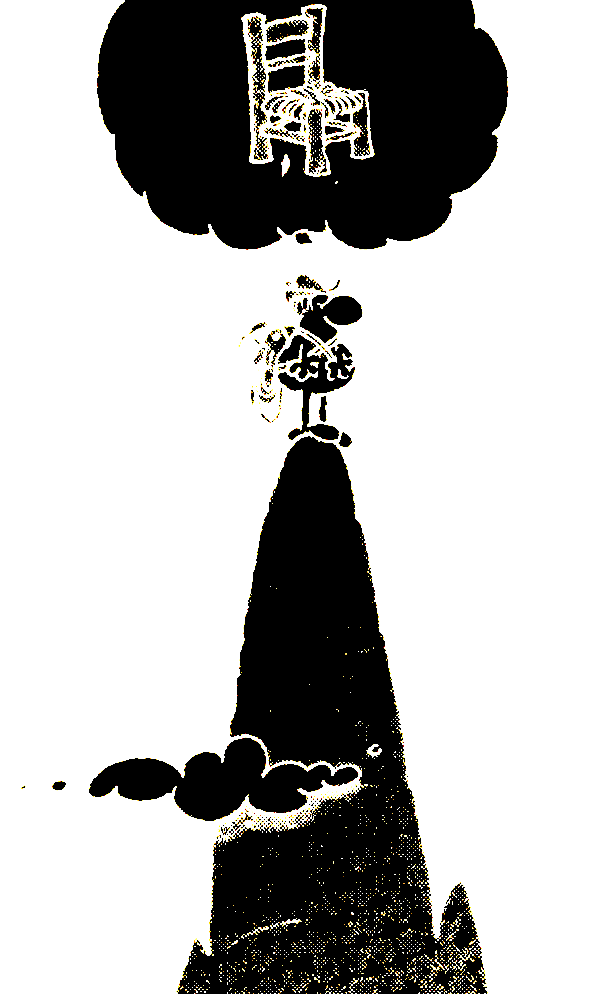
\includegraphics[height=4cm]{figures/bubbles/chair}
        \label{fig:chair}
    \end{minipage}
    \caption{Two examples by Mordillo, an artist I liked as a child: a thought bubble representing a woman, where the context of a stranded man implies a want for companionship, and a thought bubble representing a chair, where the context of a climber on a tall summit implies a want for rest.}
    \label{fig:mordillo}
\end{figure}

The visual convention for cognitive and perceptive-alethic verbs is, as far as I can tell, a kind of x-ray effect into the contents of a head, which employs the familiar container metaphor: the head is a container for thoughts.

\begin{figure}[h!]
    \centering
    \begin{minipage}[b]{0.4\textwidth}
        \centering
        
\includegraphics[height=4cm]{figures/bubbles/homer}
        \label{fig:homer}
    \end{minipage}
    \hfill
    \begin{minipage}[b]{0.4\textwidth}
        \centering
        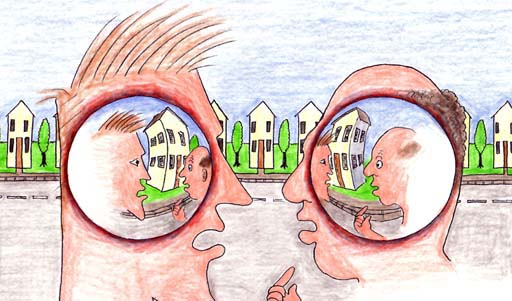
\includegraphics[height=4cm]{figures/bubbles/nestedminds}
        \label{fig:lehar}
    \end{minipage}
    \caption{On the left, a scene from the Simpsons showing the contents of Homer's mental-theatre. On the right, a depiction of two separate mental-theatres with a fisheye effect, taken from Steven Lahars "A Cartoon Epistemology" freely available online, which was also the initial inspiration for this sketch.}
    \label{fig:thinking}
\end{figure}

\begin{figure}[h!]
    \centering
    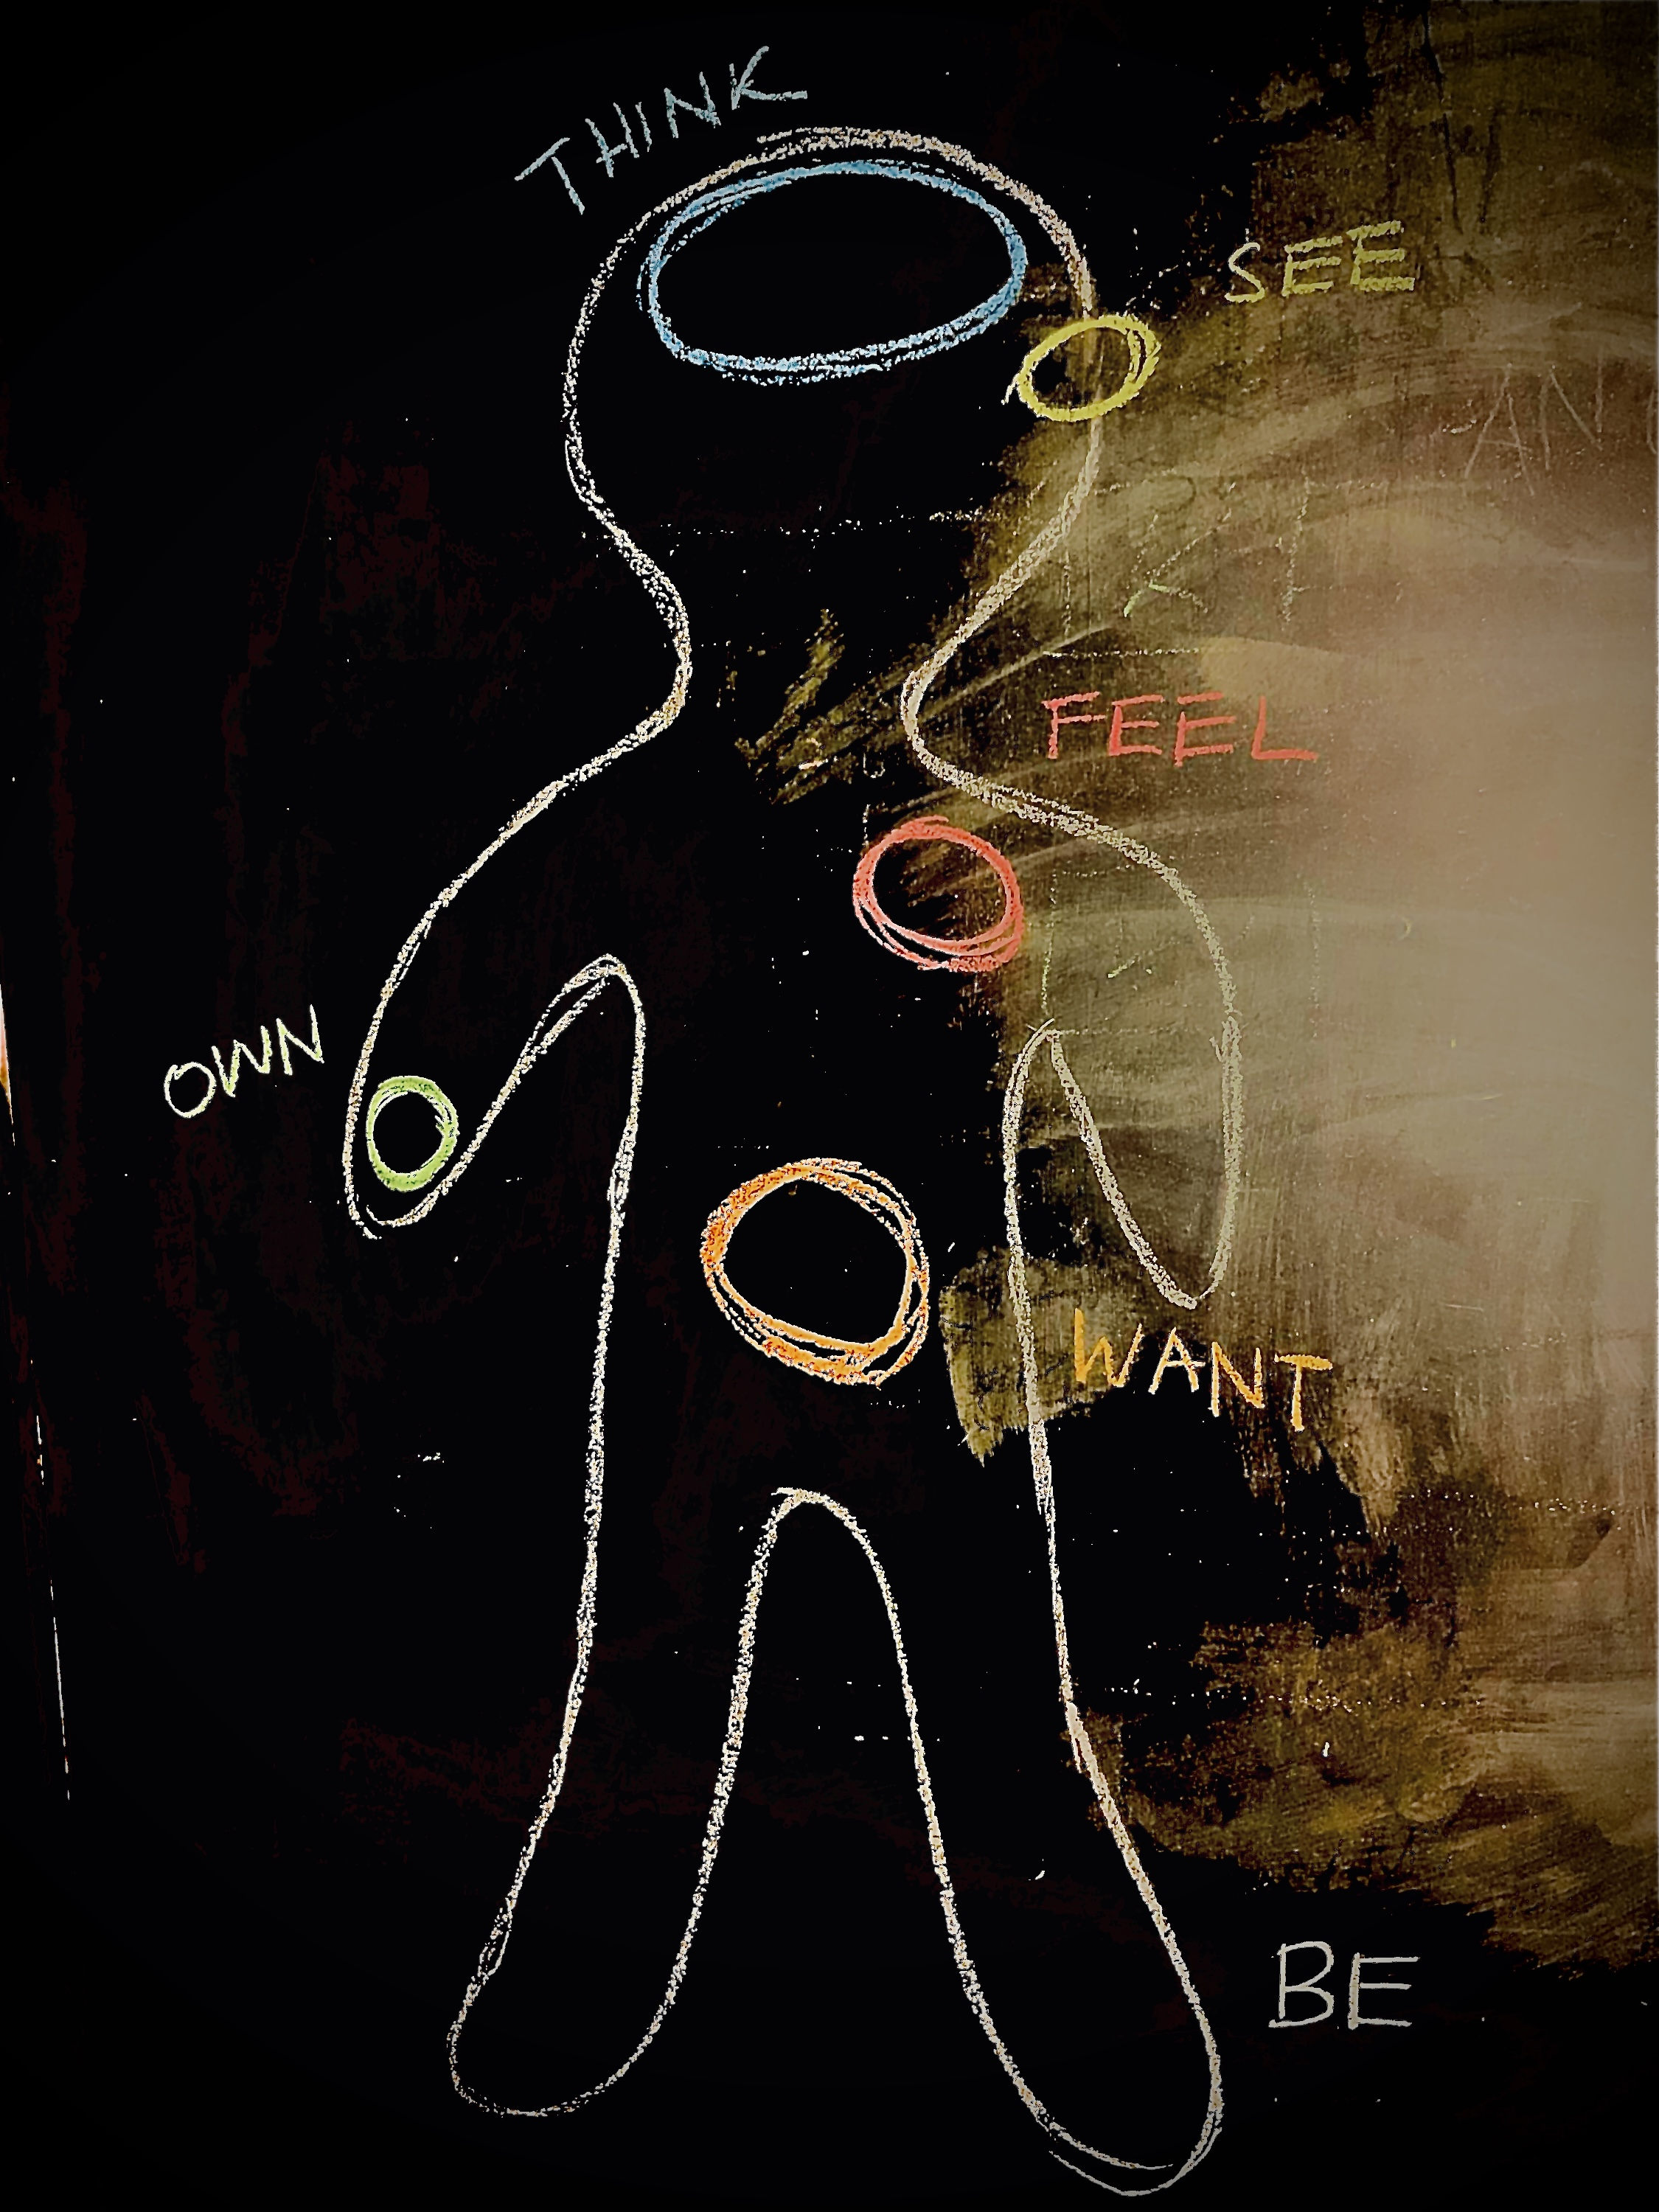
\includegraphics[height=9cm]{figures/bubbles/creepy}
    \caption{So the basic idea is to put representations of worlds inside bounded regions as containers, and in this way iconic semantics provides a univocal setting that displays all of the relevant worlds at once. We are free to pick visual conventions, as they are no more or less arbitrary than the assignment of indices and symbols such as $\mathfrak{W}_{\texttt{A}}$ to the contents of possible worlds. Here is a sketch convention for containers on an iconic representation of a person for different modal verbs: seeing, thinking, feeling, owning, and wanting. I sent this excitedly with little supporting context to Bob while I was writing my thesis. He was concerned. Then I got concerned. Childlike became creepy, and neither are good looks. I think I have supplied enough context to make this sensible, but there's no way I'm going to beat the crazy allegations.}
    \label{fig:creepy}
\end{figure}

For alethic verbs in particular (those modals that are truth-preserving, in that they "do not forget" the truth), there's a need for the contents of the container to be synchronised with the contents of the outside world. Here are some observations that enable this in \textbf{Contrel}. The basic enabling insight is that, in Euclidean spaces, if we have a hollow container with a solid blob inside, there's an approximately continuous bijection between the (open set) insides of the container and the outside world.

\clearpage

\begin{figure}[h!]
\centering
\[\scalebox{0.75}{\tikzfig{bubbles/container}}\]
\caption{The inside and the outside of a container with a solid blob inside are both homotopic to the space with a puncture. This is only approximately a continuous bijection because the unbounded outside space can only map to the open interior of the container. We can use such bijections as a bridge to establish connections between elements of different possible worlds.}
\label{fig:creepy}
\end{figure}

The second, and unfinished, idea is that if we have a handle on the individual components of sticky spiders, then we may use something like a very-well-behaved lens (hence its occurrence in the introduction) to ensure that the inside of the container is really behaving like a faithful storage medium for the goings-on outside. I think that's suggestive enough, and I'll deal with parthood in the next sketch. The last thing I want to deal with here is the problem of infinite regress for epistemic modals like knowing: if I know something, then I know I know it, and I know I know I know it, and so on. A na\"{i}ve solution is to just use an infinitely-nested series of containers.

\begin{figure}[h!]
\centering
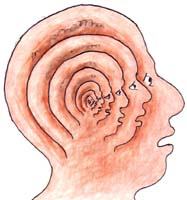
\includegraphics[height=5cm]{figures/bubbles/infinity}
\caption{Again from Cartoon Epistemology, on the unsatisfactory nature of infinitely-nested containers: \emph{But who is the viewer of this internal theatre of the mind? For whose benefit is this internal performance produced? Is it the little man at the center who sees this scene? But then how does HE see? Is there yet another smaller man inside that little man's head, and so on to an infinite regress of observers within observers?}}
\label{fig:infinity}
\end{figure}

\clearpage

So the problem here is how to encode this infinite regress with finite means in an iconic model. The usual monadic approach still runs into the problem that you have to map a potential nested-infinity of possible worlds onto some finite model if one cares about cognitive realism. In iconic semantics, we can modify the space itself; here I think Escher was onto something.

\begin{figure}[h!]
\centering
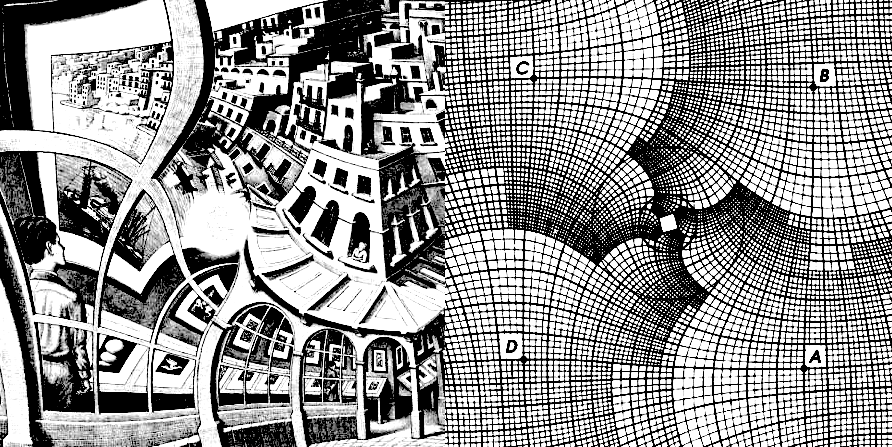
\includegraphics[height=8cm]{figures/bubbles/combined}
\caption{Escher's "Print Gallery" lithograph alongside his working sketch of the vortex-grid geometry the work was built on. On the left of the lithograph, an observer examines a framed painting of a town. Going clockwise, we see more details of the town, which has in it a print gallery, within which is the original observer. The missing centre of the piece where Escher signed the work obscures what would have been infinite nesting; the right-hand-side of the frame would have spiraled along the vortex infinitely. Treating the frame as a container, here we have an example of a container that contains itself, where movement clockwise indicates going down a level, clockwise going up, yet no explicit infinities anywhere.}
\label{fig:gallery}
\end{figure}

The space in which such an arrangement can be realised is the same as that of the Penrose staircase: splitting the lithograph into four corners, each is a locally consistent snapshot, each gluing of quadrants is a consistent (as/de)scent, but the overall manifold obtained needs to be embedded in a higher dimension. While this in principle solves the problem of finitely representing infinite descent, these kinds of spaces are not grounded in physical, embodied intuitions. I think it is mathematically neat that there can exist topological models for such modal verbs, but whether such proposals are to be taken seriously as modelling cognition is a thorny matter I don't want to say more about.
\clearpage
\newpage
\section{Iconic semantics for general anaphora via Turing objects}

This sketch complements the sketch on modals, as it relies on the same container-trick. I would like to explain here how iconic semantics in \textbf{ContRel} might model untyped-boxes --- these are conjunctions and verbs with sentential complements --- as well as the more general linguistic phenomena of \emph{entification} and \emph{general anaphora} --- where arbitrary discourse elements up to collections of sentences may be packaged up as if they were nouns and referred to. I suggest that the mathematical property of \textbf{ContRel} that enables this is that it contains \textbf{FinRel} equipped with a \emph{Turing object}.

\newthought{Entification is the process of turning words and phrases that aren't nouns into nouns.} We are familiar with morphological operations in English, such as \emph{inflections} that turn the singular \texttt{cat} into the plural \texttt{cats}, by adding a suffix \texttt{-s}. Another morphological operation generally called \emph{derivation} changes the grammatical category of a word: for example, the adjective \texttt{happy} derives the noun \texttt{happiness}. With suffixes such as \texttt{-ness} and \texttt{-ing}, just about any lexical word in English can be turned into a noun, as if lexical words have some semantic content that is independent of the grammatical categories they might wear as a guise. With more complex discourse prefixes such as \texttt{the fact that}, we may also disguise sentences and text as nouns.

\begin{example}{Generalised anaphora as entification.}
\[\texttt{Jono is paid minimum wage. He didn't mind \textcolor{cyan}{it}.}\]
\[\tikzfig{spatialencoding/jono}\]
An example of entification. It may be argued that \textcolor{cyan}{\texttt{it}} refers to \texttt{the fact that Jono was paid minimum wage}. Graphically, we might want to depict the gloss as a circuit with a lasso that gives another noun-wire that encodes the information of the lassoed part of the circuit.
\end{example}

The problem at hand is finding an appropriate mathematical setting to interpret and calculate with such lassos. In principle, any meaningful (possibly composite) part of text can be referred to as if it were a noun. For syntax, this is a boon; having entification around means that there is no need to extend the system to accommodate wires for anything apart from nouns, so long as there is a gadget that can turn anything into a noun and back. For semantics this is a challenge, since this requires noun-wires to "have enough space in them" to accommodate full circuits operating on other noun-wires, which suggests a very structured sort of infinity. Computer science has had a perfectly serviceable model of this kind of noun-wire for a long time. What separates a computer from other kinds of machine is that a computer can do whatever any other kind of machine could do --- modulo church-turing on computability and the domain of data manipulation --- so long as the computer is running the right \emph{program}. Programs are (for our purposes) processes that manipulate variously formatted --- or typed --- data, such as integers, sounds, and images. They can operate in sequence and in parallel, and wires can be swapped over each other, so programs form a process theory, where we can reason about the extensional equivalence of different programs --- whether two programs behave the same with respect to mapping inputs to outputs. What makes computer programs special is that on real computers, they are specified by \emph{code}. Programs that are equivalent in their extensional behavior may have many different implementations in code: for example, there are many sorting algorithms, though all of them map the same inputs to the same outputs. Conversely, every possible program in a process theory of programs must have some implementation as code. Importantly, code is just another format of data. The process-theoretic characterisation of the code-wire in a process-theory of computation is this:
\marginnote{
Another observation we could have made is that since computers really just manipulate code, every data format is a kind of restricted form of the same Turing object $\Xi$, but this turns out to be a mathematical consequence of the above equation (and the presence of a few other operations such as copy and compare that form a variant of frobenius algebra), demonstrated in Pavlovic's forthcoming monoidal computer book \citep{pavlovic_programs_2023}, itself a crystallisation of three monoidal computer papers \citep{pavlovic_monoidal_2012,pavlovic_monoidal_2014,pavlovic_monoidal_2018}. I would be remiss to leave out Cockett's work on Turing categories \citep{cockett_introduction_2008}, from which I took the name Turing object. Both approaches to a categorical formulation of computability theory share the common starting ground of a special form of closure (monoidal closure in the case of monoidal computer and exponentiation in Turing categories) where rather than having dependent exponential types $\mathbb{A} \multimap \mathbb{B}$ or $\mathbb{B}^\mathbb{A}$, there is a single "code-object" $\Xi$. They differ in the ambient setting; Pavlovic works in the generic symmetric monoidal category, and Cockett with cartesian restriction categories, which generalise partial functions. I work with Pavlovics' formalism because I prefer string diagrams to commuting diagrams.}
\begin{defn}[Turing object]\label{defn:turing}
A \emph{Turing object} $\Xi$ in a process-theory is equipped with evaluation morphisms $\text{ev}^{A}_{B} : A \otimes \Xi \rightarrow B$ for all pairs of objects $A,B$ such that for all morphisms $f: A \rightarrow B$, there exists a state $\ulcorner \! f \urcorner_{: I \rightarrow \Xi}$ of the Turing object such that partial evaluation with that state is equal to $f$. The diagrammatic convention and visual pun \citep{pavlovic_programs_2023} for such code-states and evaluators is to depict the state-triangle as if it is cut out from the rectangle of the evaluator.
\[
\forall A,B \in Ob(\mathcal{C}) \ \exists \text{ev}^{ A}_{B} \ \forall f \ \exists \ulcorner \! f \urcorner\]
\[
\tikzfig{spatialencoding/eval}
\]
\end{defn}

Any programming language is a model for text circuits, using the code-data format as the noun wire and Turing object. In \textbf{ContRel}, the unit square suffices as a Turing object for finite sets and relations, as we can use the container-trick of modals.

\begin{proposition}[Sticky spiders on the open unit square model \textbf{FinRel} equipped with a Turing object]
Using the open unit square with its usual topology as the Turing object, there is a subcategory of \textbf{ContRel} which behaves as the category of countable sets and relations equipped with a Turing object
\begin{proof}
By Construction \ref{cons:unitencoding}, which we work towards.
\end{proof}
\end{proposition}

\begin{lemma}[$(0,1) \times (0,1)$ splits through any countable set $X$]
For any countable set $X$, the open unit square $\squarehvfill$ has a sticky spider that splits through $X^\star$ --- the discrete topology on $X$.
\begin{proof}
Proof by construction. Assume we work with nice spiders, so we only have to highlight the copiable open sets. Take some circle and place axis-aligned open squares evenly along them, one for each element of $X$. The centres of the open squares lie on the circumference of the circle, and we may shrink each square as needed to fit all of them.
\[\scalebox{1}{\tikzfig{spatialencoding/circencodingconstruct}}\]
\end{proof}
\end{lemma}

\begin{defn}[Morphism of sticky spiders]
A morphism between sticky spiders (here cyan and magenta) is any continuous relation that satisfies the following equation.
\[\scalebox{1}{\tikzfig{spatialencoding/stickymorphismdefn}}\]
\end{defn}

\begin{lemma}[Morphisms of sticky spiders encode relations]
For arbitrary split idempotents through $A^\star$ and $B^\star$, the morphisms between the two resulting sticky spiders are in bijection with relations $R: A \rightarrow B$.
\[\resizebox{\textwidth}{!}{\tikzfig{spatialencoding/arbsetclaim}}\]
\begin{proof}
\[\resizebox{\textwidth}{!}{\tikzfig{spatialencoding/arbset}}\]
\end{proof}
\end{lemma}

\begin{construction}[Representing sets in their various guises within $\squarehvfill$]
We can represent the direct sum of two $\squarehvfill$-representations of sets as follows.
\[\scalebox{0.75}{\tikzfig{spatialencoding/directsumconstruct}}\]
The important bit of technology is the homeomorphism that losslessly squishes the open unit square into one half of the unit square. The decompressions are partial continuous functions, with domain restricted to the appropriate half of the unit square.
\[\scalebox{1}{\tikzfig{spatialencoding/leftrightcompressions}}\]
We express the ability of these relations to encode and decode the unit square in just either half by the following graphical equations.
\[\scalebox{1}{\tikzfig{spatialencoding/leftrightcompressions2}}\]
\end{construction}
Now, to put the two halves together and to take them apart, we introduce the following two relations. In tandem with the squishing and stretching we have defined, these will behave just as the projections and injections for the direct-sum biproduct in \textbf{Rel}.
\[\resizebox{\textwidth}{!}{\tikzfig{spatialencoding/leftrightcompressions3}}\]
The following equation tells us that we can take any two representations in $\squarehvfill$, put them into a single copy of $\squarehvfill$, and take them out again.
\[\scalebox{1}{\tikzfig{spatialencoding/leftrightcompressions4}}\]

We encode the tensor product $A \otimes B$ of representations by placing copies of $B$ in each of the open boxes of $A$.
%\[\scalebox{0.75}{\tikzfig{spatialencoding/directsummap}}\]
%\[\scalebox{0.75}{\tikzfig{spatialencoding/directsummap2}}\]
\[\scalebox{0.75}{\tikzfig{spatialencoding/tensorconstruct}}\]
The important bit of technology here is a family of homeomorphisms of $\squarehvfill$ parameterised by axis-aligned open boxes, that allow us to squish and stretch spaces. Thus for every representation of a set in $\squarehvfill$ by a sticky-spider, where each element corresponds to an axis-aligned open box, we can associate each element with a squish-stretch homeomorphism via the parameters of the open box, which we notate with a dot above the name of the element.
\[\resizebox{\textwidth}{!}{\tikzfig{spatialencoding/compresstogether}}\]

Now we can define the "tensor $X$ on the left" relation $\_ \rightarrow X \otimes \_$ and its corresponding cotensor.
\[\resizebox{\textwidth}{!}{\tikzfig{spatialencoding/tensordetensor}}\]
The tensor and cotensor behave as we expect from proof nets for monoidal categories.
\[\resizebox{\textwidth}{!}{\tikzfig{spatialencoding/tensordetensor2}}\]
And by construction, the (co)tensors and (co)pluses interact as we expect, and they come with all the natural isomorphisms between representations we expect. For example, below we exhibit an explicit associator natural isomorphism between representations.
\[\scalebox{1}{\tikzfig{spatialencoding/tensordetensor3}}\]

\begin{construction}[Representing relations between sets and their composition within $\squarehvfill$]\label{cons:unitencoding}
With all the above, we can establish a special kind of process-state duality; relations as processes are isomorphic to states of $\squarehvfill$, up to the representation scheme we have chosen. This is part of the condition for Turing objects. What remains to be demonstrated is that the duality coheres with sequential and parallel relational composition.
\end{construction}
\[\scalebox{0.9}{\tikzfig{spatialencoding/relcomp1}}\]
Under this duality, we have continuous relations that perform sequental composition of relations as follows.
\[\resizebox{\textwidth}{!}{\tikzfig{spatialencoding/relcomp2}}\]
And similarly, parallel composition. Therefore, we have demonstrated that the unit square behaves as a Turing object for the category of countable sets and relations.
\[\resizebox{\textwidth}{!}{\tikzfig{spatialencoding/relcomp3}}\]
\clearpage
\newpage
\section{Configuration spaces}
\marginnote{Configuration spaces and possible-worlds semantics favour working string-diagrammatically in \textbf{ContRel} over \textbf{Top}. The latter's cartesian monoidality limits it to one effect (delete) and only tensor-separable states, preventing native diagrammatic reasoning about correlated states analogous to entangled quantum states and spatial relations \citep{coeckePicturingQuantumProcesses2017a, wang-mascianicaTalkingSpaceInference2021a}.
The Fregean notion of compositionality --- knowing a composite system is equivalent to knowing all its parts --- corresponds to tensor-separability in cartesian monoidal categories. Schr\"{o}dinger's quantum mechanics insight offers an alternative: perfect knowledge of the whole doesn't necessitate perfect knowledge of the parts \citep{coeckeCompositionalityWeSee2021}.
Information about a composite system restricts possible outcomes a priori. The bell-state exemplifies this: we know both qubits measure identically, but discarding one qubit leaves maximal entropy for the remaining one. Similarly, imagining "a cup on a table in a room" entangles the objects' positions. Removing either object eliminates restrictions on the other's location, demonstrating that meaning resides in the entangled whole rather than individual parts.}
Individual sticky-spiders correspond to static collections of set-labelled shapes in \textbf{ContRel}; in this sketch I want to talk about all the different ways the same collection of shapes can be arranged in space.

Let's also say we start with the ability to detect whether two sticky-spiders are related to one another by rigid displacements, expressed as a topological group with elements we denote $\rho$. Since sticky-spiders can be represented as unions of effects followed by states, we can define a binary relation on sticky-spiders that tells us whether they are the same up to rigidly displacing component shapes:

\begin{defn}[Displacement relation]
Two sticky-spiders (cyan and green, both assumed to be nice here), each with components indexed by $I$, are \emph{equivalent up to displacement} when there exist $\rho_i$ such that:
\[\resizebox{\textwidth}{!}{\tikzfig{topology/displacementrelation}}\]
We've suppressed labelling of the states and we've contracted the cup to just depict the open state as a semicircle.
\end{defn}

Displacement is evidently an equivalence relation, and moreover requires that the two spiders related have the same number of components. Now given a particular nice spider, we treat its equivalence class of spiders as a configuration space in which we have access to all of its rigidly displaced variants at once.

\begin{defn}\label{defn:configurationspace}
The \emph{configuration space} $C(\mathfrak{s})$ of a nice spider $\mathfrak{s}$ with indexing set $I$ is the topological space with underlying set defined to be the equivalence class $[\mathfrak{s}]$ of $\mathfrak{s}$ under displacement. Assuming the topological group of rigid displacements is itself a topological space $G$, the topology of $C(\mathfrak{s})$ is a restriction of $\bigtimes^{|I|} G$ to those $|I|$-tuples of displacements witnessed by $[\mathfrak{s}]$.
\end{defn}

\begin{example}[The connected components of configuration space]
Configuration space allows us to define a "slideability" relation between configurations of a spider $\mathfrak{k}$ as the endpoints of continuous functions from the unit interval into $C(\mathfrak{s})$. This in turn allows us to consider what the connected components of configuration space are. Evidently, there are pairs of spiders that are both valid displacements, but not mutually reachable by sliding. For example, shapes might \emph{enclose} or \emph{trap} other shapes, or shapes might be \emph{interlocked}. So at first blush, the connected components of configuration space tells us something about holes, or the cohomology of configurations. Depicted are some pairs of configurations corresponding to some linguistically topological terms that are mutually unreachable by rigid transformations, and so must live in disconnected components of configuration space.
\[\resizebox{\textwidth}{!}{\tikzfig{topology/encloseexample}}\]
\end{example}

In configuration spaces we're making use of the fact that any displacement relationship comes with (up to a non-unique choice of basepoints for each component shape)  a witnessing tuple of $\rho_i$s. As a consequence, the configuration space of a sticky-spider is a retract of the product space $\bigtimes^{|I|} G$ where $G$ is the topological group of displacements, and we can use the identity relation between the section and retraction to strip the configuration space wire, revealing each of the $\bigtimes^{|I|} G$ like guitar strings: each element of the set that the initial nice spider $\mathfrak{s}$ splits through gets its own string.
\[\tikzfig{topology/guitar}\]
Note that although every guitar string is $G$, there is extra typing data indicating which element of the indexing set of the spider each $G$ corresponds to. So here's a model in which the named wires of text circuits make sense. We can put gates on the guitar strings, which may for example correspond to constraints on the relative positions of shapes in configuration space.
\[\tikzfig{topology/guitargate}\]

The next thing we can try is to add and subtract shapes from configuration spaces, and while there are technical details like matching choices of basepoints I'll gloss over, the gist is this: when the shapes in a nice spider $\mathfrak{s}$ are a subset of the shapes in a nice spider $\mathfrak{t}$, we can add in states to the guitar-picture of $\mathfrak{s}$ and wrap them up again using the idempotent of $\mathfrak{t}$, and we can delete wires in the guitar-picture of $\mathfrak{t}$ and wrap that up using the idempotent of $\mathfrak{s}$.

\[\tikzfig{topology/addminus}\]

The last stop in this sketch is disintegrating and integrating shapes; if we could freely break apart a shape, we know that in principle we get another configuration space where we can manipulate those parts, and if we can glue those pieces back together again, then we could do simple things like open and close containers. Let's first define the disintegration relation between spiders. Observe that the data of a nice spider is equivalently viewed as a function $f: I \rightarrow \mathfrak{O}$, where $I$ is the indexing set, and $\mathfrak{O}$ is some set of opens with whatever well-behaviour condition, along with the constraint that $f(x) \cap f(y) \neq \varnothing \Rightarrow x = y$ that enforces non-overlapping shapes. This perspective gives us a foothold to define a disintegration relation: a "more refined" spider is one that has a superset of $I$ as domain, with a function that sends elements of the indexing set to either the same shape as $f$, or a subshape.

\begin{defn}[Disintegration]
Let $\mathfrak{s}$ and $\mathfrak{t}$ be nice spiders, described by functions $s: I \rightarrow \mathfrak{O}$ and $t: J \rightarrow \mathfrak{O}$ respectively. $\mathfrak{t}$ \emph{disintegrates} $\mathfrak{s}$ ($\mathfrak{t} \succ \mathfrak{s}$) if there exists a surjective $d: J \twoheadrightarrow I$ such that $g = f \circ d$, and such that for all $i \in I$ and all $j \in d^{-1}(i)$, $g(j) \subseteq f(i)$.
\end{defn}

Since the composition of surjectives is also surjective and the subsethood condition is transitive, disintegration is a transitive relation. It's also reflexive, and since surjections $A \twoheadrightarrow B$ and $B \twoheadrightarrow A$ implies a bijection $A \simeq B$ and $X \subseteq Y$ with $Y \subseteq X$ implies $X = Y$, we also have antisymmetry, and hence a partial order. Treating the identity disintegration as globally minimal, we can define shatterings as locally minimal elements.

\begin{defn}[\emph{Solve}]
$\mathfrak{t}$ \emph{shatters} $\mathfrak{s}$ if $\mathfrak{t} \succ \mathfrak{s}$, and for all spiders $\mathfrak{q}$, $\mathfrak{t} \succ \mathfrak{q} \succ \mathfrak{s} \Rightarrow \mathfrak{q} = \mathfrak{t}$ or $\mathfrak{q} = \mathfrak{s}$, up to bijective relabellings of indexing sets.
\end{defn}

The intuition behind shattering is that the $\subseteq$-condition in the disintegration relation lets the disintegrating spider "shave a little" off of the disintegrated spider, and locally minimal disintegrations "shave the least off", doing the best they can to partition shapes. So now we get gluing for free:

\begin{defn}[\emph{et Coagula}]
$\mathfrak{t}$ is a \emph{gluing} of $\mathfrak{s}$ if $\mathfrak{s}$ shatters $\mathfrak{t}$.
\end{defn}

\begin{example}[Putting something in a container]
To put a blob inside a container, we first shatter the container of the initial spider $\mathfrak{s}$ to obtain a new spider $\mathfrak{t}$ that expresses the container as a combination of a container and a lid, then (implicitly using dynamic verb composition of terminatives) we can move the lid, put the blob in, close the lid, and glue. Below the circuit we represent one possible series of consistent snapshots as a vignette, out of the many possible series of configurations that satisfy our linguistic description above.
\[\tikzfig{topology/containervignette}\]
In principle, shapes can be shattered arbitrarily finely, which permits us some degree of freedom in specifying how a container opens. In conjunction with a topological group of transformations that includes scaling, we may express different ways in which things get in and out of containers, or otherwise leave the original connected component of configuration space they start in. Here again I'm colour coding different shapes of the same spider with different colours.
\[\resizebox{\textwidth}{!}{\tikzfig{topology/inopenout}}\]
\end{example}

I'll close this sketch with something cute: if manipulating shapes in configuration space is serious and sensible stuff, then just about anything is. We can (ab)use the fact that shapes of a nice sticky spider do not overlap to model mechanical components, where acceptable configurations of different shapes are mutually constrained in a productive way. In particular, this means we may consider any linguistic semantics grounded in mechanical or boardgame-tabletop models to be formal: in principle anything that can be represented by mechanisms and meeples is fair game\marginnote{\textsc{Objection: Isn't this way outside the scope of formal semantics?} Insofar as semantics is sensemaking, we certainly are capable of making sense of things in terms of mechanical models and games by means of metaphor, the mathematical treatment of which is concern of Section \ref{sec:metaphor}. It's probably the case that any definition that encompasses what's going on here as formal semantics would also have to consider the programming of a videogame to also be a form of formal semantics; personally I think that's ok, because I don't consider any particular form of mathematics-as-methodology to be privileged over others. Feel free to disagree.}. This gives us some cool possibilities for formal models of natural language, as there are a lot of mechanical models, including: clocks [duh.], analogues of electric circuits \citep{SpintronicsBuildMechanical}, computers \citep{richardridelMechanicalTuringMachine2015}, and human-like automata \citep{wikipediaauthorsJaquetDrozAutomata2022}.

\begin{example}[Mechanical semantics]
Here I'm going to allow shapes to be unions of disjoint contractibles, and I'll colour-code the different shapes in the spiders differently so the different components are clear:
\[\resizebox{\textwidth}{!}{\tikzfig{topology/constrained}}\]
%Of course in reality mechanical motions are reversible among rigid objects, and directional behaviour is provided by a source of energy, such as gravitational potential, or wound springs. But we may in principle replace these sources of energy by a belt that we choose to spin in one direction -- our own arrow of time.
\end{example}
\clearpage
\newpage
\section{Formal models from figurative language}\label{sec:metaphor}

Figurative language is when language is used non-literally, e.g. \texttt{to bathe in another's affection}. Figurative language subsumes analogy (\texttt{built like a mountain}), metaphor (\texttt{she got a lot out of that lecture}) and some idioms (\texttt{raining cats and dogs}). The issue with figurative language for formal semantics, insofar as formal semantics is concerned with truth-conditions, is that one requires an underlying model in order to begin truth-conditional analysis. The role of figurative language, especially that of metaphor, is in some sense to provide those models in the first place\marginnote{\citep{reddy_conduit_nodate} argues convincingly that the metaphor \texttt{IDEAS are CONTAINERS} is pervasive in English; it is just about the only way we talk about communication. Yet there is no literal sense in which one can 'get something' out of a lecture or 'pack a lot' into a book. Evidently the \emph{systematicity of the metaphor itself} yields the common structure from which we can even begin to consider pedestrian truth-conditional analyses; i.e. language has a role to play in constructing the stage, and afterwards we can reason logically about the actors and events. The process by which language constructs the underlying model is not by nature truth-conditional: there is no fact of the matter before it is read of a fictional character's eye-colour, but it does become a facet of the reader's world-model afterwards. Therefore: of which truth-conditions cannot speak, thereof truth-conditionalists must remain silent.}, so the truth-theoretic (or inquisitive, or dynamic) approach to semantics operates at an inappropriate stage of abstraction. We might illustrate or depict schema to represent figurative language, but to the best of my knowledge, there is no formal account of how the systematicity of a chosen schematic corresponds to the organisation of a metaphor or concept. So what is required is a methodology to construct the underlying models from the figurative language in a more-or-less systematic way.\\

The whole point of mucking around with \textbf{ContRel} earlier is this: figurative language can be formally interpreted as vignettes involving topological figures. I will demonstrate here that cofunctors from \textbf{ContRel} into text-circuits representing utterances are promising candidates for the formalisation of figurative language. My focus will exclude idiomatic language and one-off analogies in favour of metaphor just because the latter is most interesting, though the methodology applies in other cases of figurative language. I will take a \emph{metaphor} to be figurative language that utilises the systematic structure in one conceptual domain to give partial structure in another conceptual domain\marginnote[1cm]{Meta, beyond. Phor, as in amphora, an agent, carrier, or producer. Metaphor carries meaning beyond one domain to another. It bears and produces meaning. Metaphors are the primary agents of meaning.}. This may subsume some cases of what would otherwise be called \emph{similes} or \emph{analogies}. The differences far as I can tell between a metaphor and an analogy is the presence of systematicity in the former, and a weak requirement that the correspondence involves separate conceptual domains. It doesn't really matter for this discussion what the difference is.\\

First, we observe that we can model certain kinds of analogies between conceptual spaces by considering structure-preserving maps between them. For example, Planck's law gives a partial continuous function from part of the positive reals measuring tempature of a black body in Kelvin to wavelengths of light emitted, and the restriction of this mapping to the visible spectrum gives the so-called "colour temperature" framework used by colourists. It will turn out that a decategorified cofunctor has the right kind of structure.\\

Second, we observe that we can use simple natural language to describe conceptual spaces, instead of geometric or topological models. Back to the example of colour temperature, instead of precise values in Kelvin, we may instead speak of landmark regions that represent both temperature and colour such as \texttt{incandescent} and \texttt{daylight}, which obey both temperature-relations (e.g. \texttt{incandescent is cooler than daylight} and colour-relations (e.g. \texttt{daylight is bluer than incandescent}).\\

Third, we observe that we can also use simple natural language to describe more complex conceptual schemes with interacting agents, roles, objects, and abilities. This will require a cofunctor. Organising this linguistic data in the concrete structure of a text circuit allows us to formally specify what it means for one conceptual scheme to structure another by describing structure-preserving maps between the text circuits. This will allow us construct topological models of metaphors such as \texttt{TIME is MONEY}.

\subsection{Temperature and colour: the Planckian Locus}

\begin{example}[The Physicists' Planckian Locus]\label{ex:planck1}
Planck's law describes the spectral radiation intensity of an idealised incandescent black body as a function of light frequency and temperature. Integrating over light frequencies in the visible spectrum yields a function from temperature of the black body to chromaticity.
\begin{figure}[h]
\centering
\scalebox{0.5}{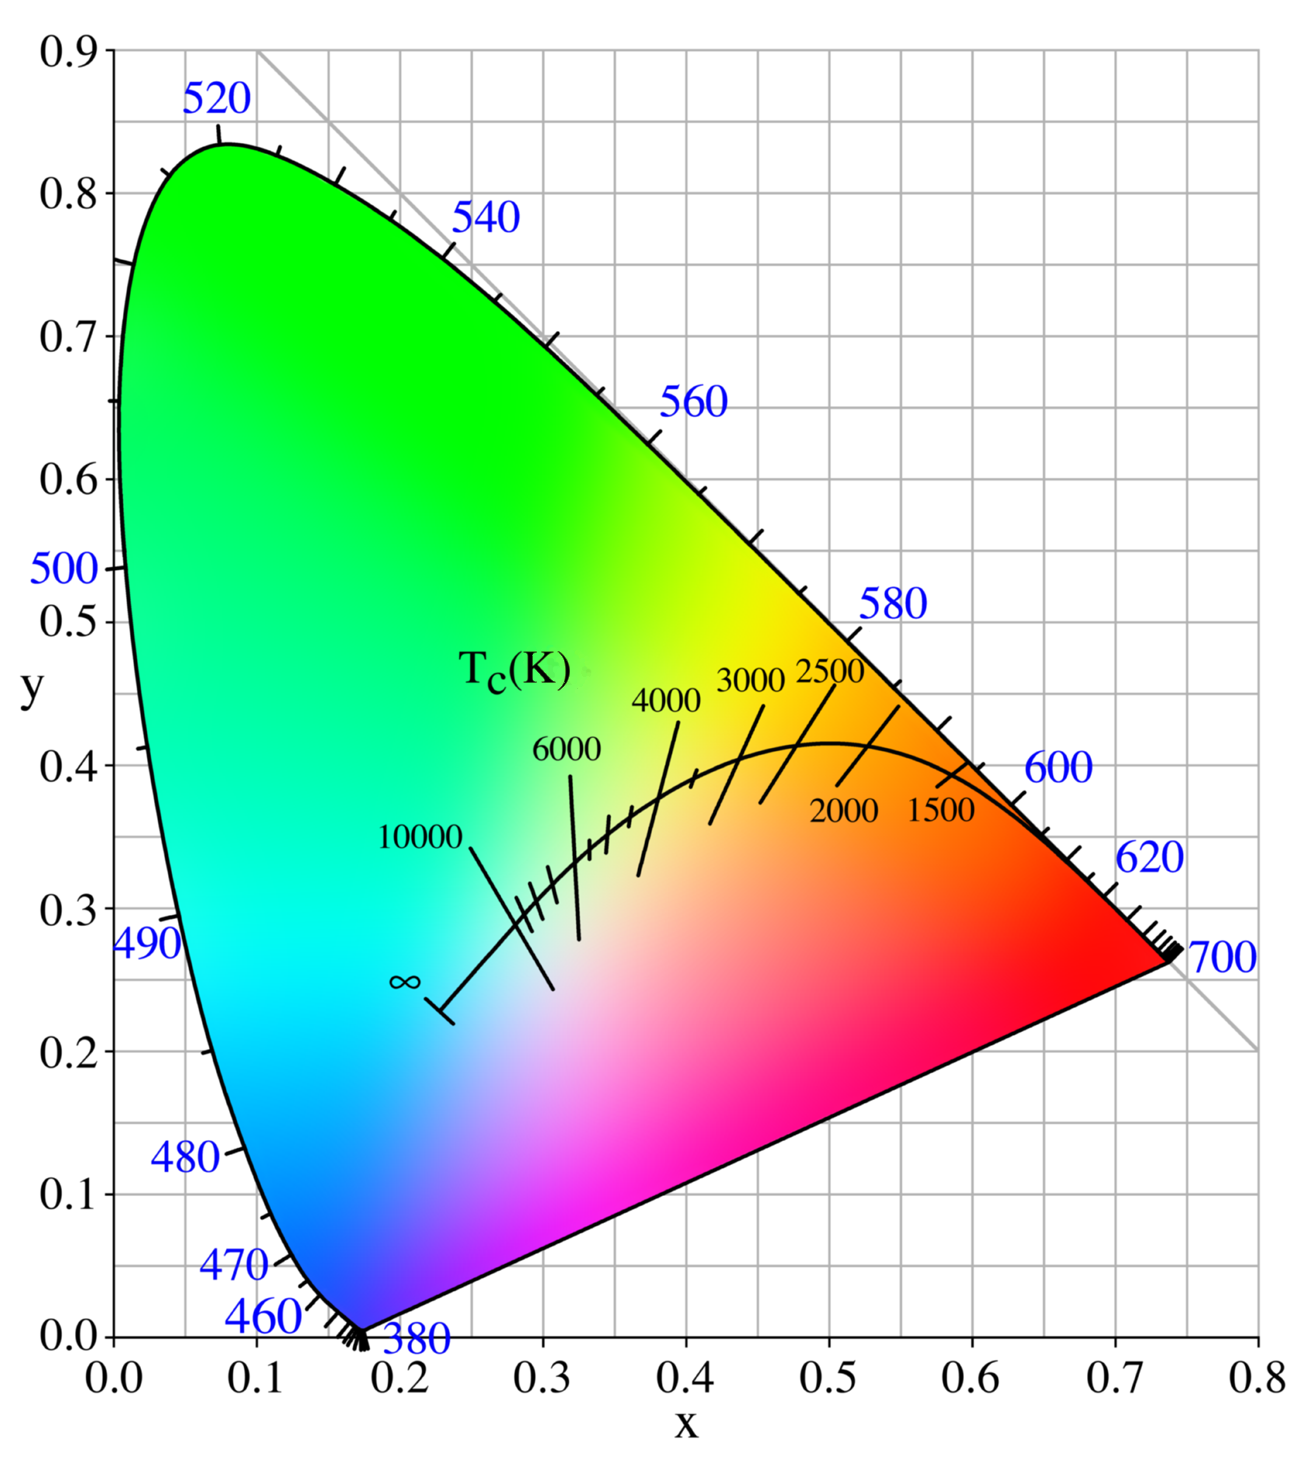
\includegraphics{figures/metaphor/PlanckianLocus}}
\caption{The Planckian Locus in the CIE 1931 chromaticity diagram. Chromaticity refers only to the hue of a colour, without other domains such as saturation.}
\end{figure}
\end{example}

Abstractly, the Planckian Locus is a continuous function mapping the positive real line representing the conceptual domain of temperature into the plane representing the conceptual domain of colour. The Planckian locus is the basis of colourist-talk about colour schemes in terms of temperature, which allows them to coordinate movements in colourspace using the terminology of temperaturespace, e.g. \texttt{make this shot warmer}. This fits with what we would prototypically expect a metaphor to allow us to do with meanings.

However, the particular mathematical conception of metaphor-as-map in Example \ref{ex:planck1} is too rigid: it only goes one way. It is a specific and inflexible kind of metaphor that does not behave at all outside its specified boundaries. For example, colourists have to deal with offsets towards green and magenta, which are not in the chromaticity codomain of the function given by Planck's law. It would be truer to life if we further analysed the function as mediated by a strip.

\begin{example}[The colourist's Planckian Locus]
Now we aim to extend our mathematical model to accommodate the fact that colourists deal with chromatic offsets or deviations from the mathematically precise locus given by Planck's law.
\begin{figure}[h]
\centering
\scalebox{0.5}{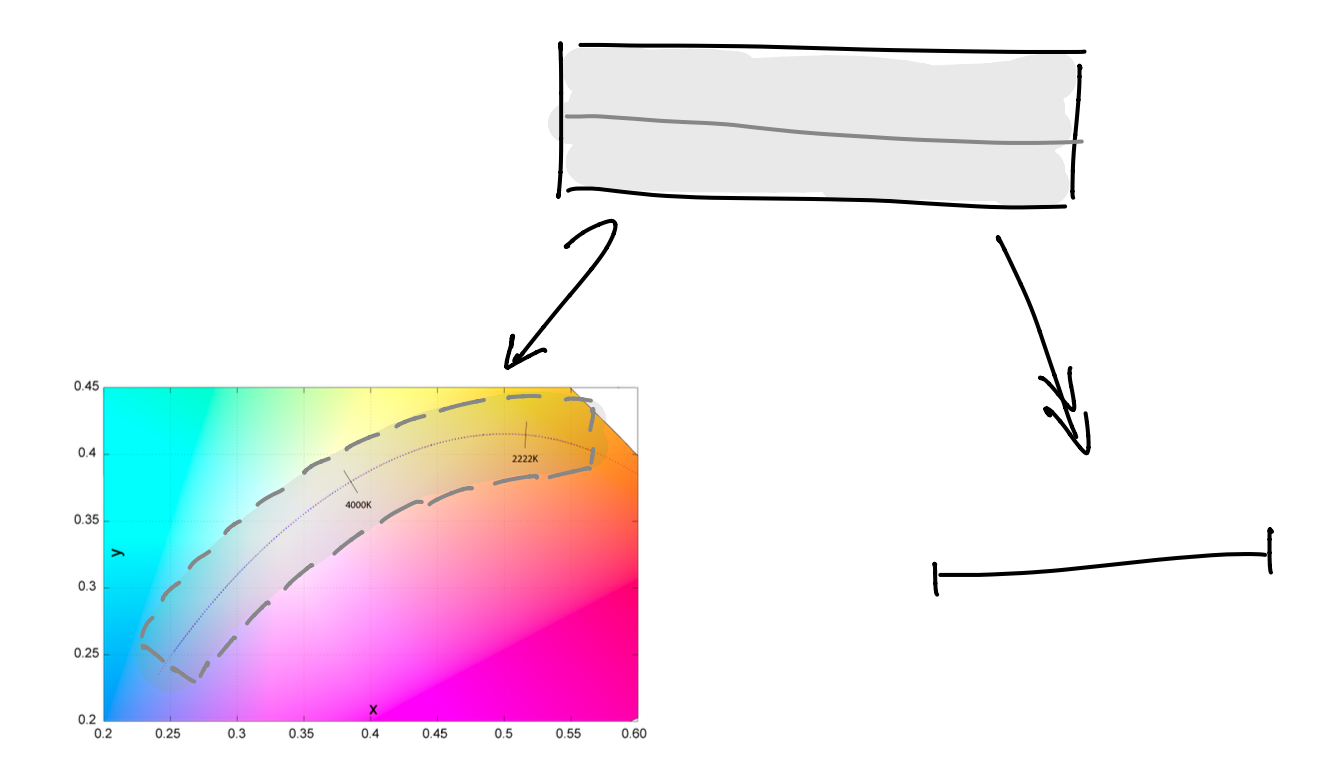
\includegraphics{figures/metaphor/colourlocus1}}
\caption{Consider the unit square (depicted as a strip) as a fiber bundle over the unit interval representing temperature range. There is an injective continuous map from the strip into colourspace that is centered on the Planck Locus.}
\end{figure}
\begin{figure}[h]
\centering
\scalebox{0.5}{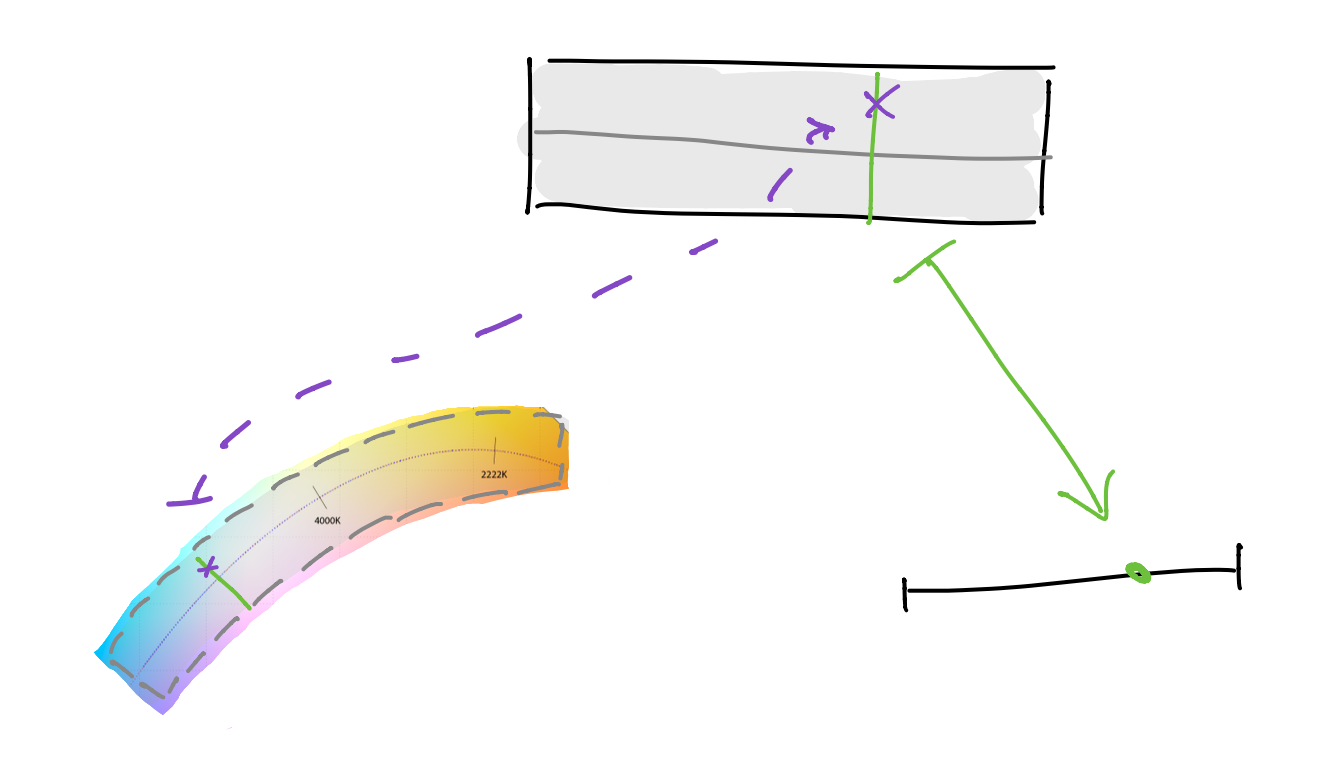
\includegraphics{figures/metaphor/colourlocus2}}
\caption{The left leg is bijective in the image restriction, so any point or displacement in the offset-strip in colourspace can be lifted to a point in the apex strip, which is then projected down along with other points in the vertical fiber to a point in temperaturespace. So we have a decategorified cofunctor!}
\end{figure}
\end{example}

A refinement we have just captured is the partially-structuring nature of metaphor \citep{lakoff_metaphors_2003}. In the language of our running example, pure green is outside the scope of the colour-temperature correspondence given by the Planckian Locus, so the metaphor is only a partial structuring of the colour domain according to the temperature domain. This partiality in the colour domain means that it would have been inappropriate to model the passage of colour-talk to temperature-talk as a function from colour to temperature, as functions are total, rather than partial, on their domain. While it is conceptually nice that we are on the way to recovering monoidal cofunctors as a model of metaphor, why didn't we stay simple and just use a partial function? The answer is that the strip at the apex represents the \emph{talk} part of colour- and temperature-talk.

\begin{example}[Conceptual transfer between domains]
When colourists use the temperature metaphor they might say "hot", "warm", "cooler", which are not specific temperature ranges in Kelvin, but concepts in temperature-space. Recalling that we may consider concepts to be open sets of a topology (and comparatives as opens of the product), we observe that we can linguistically model regions on the positive reals with words \texttt{little} (labelled $l$), \texttt{lot} (labelled $L$), and \texttt{more} (labelled $M$), an algebraic basis from which derive \texttt{less} by symmetry, and other regions such as \texttt{more than a little, less than a lot}. In this particular running example, it happens that both legs of the span of functors have a lifting property, which explains how we might model the fact that conceptual colourist-talk of "daylight" or "candlelight" in the colour domain can be sensibly interpreted in the temperature domain. The formalisation of this fact follows by symmetry from this example.
\begin{figure}[h]
\centering
\resizebox{0.8\textwidth}{!}{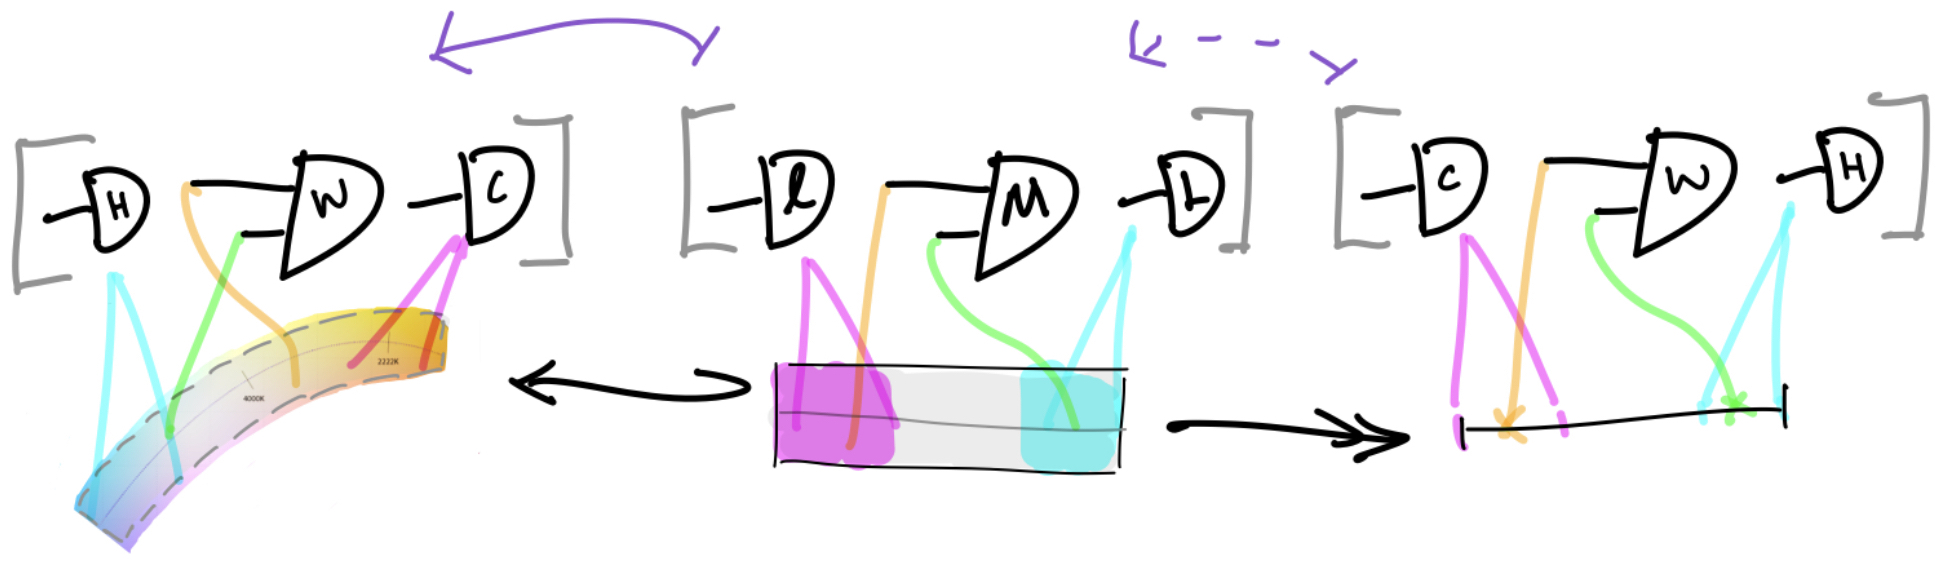
\includegraphics{figures/metaphor/offset1.jpeg}}
\caption{Starting from the right, the lifting property of the right leg is what lets us map "hotter and colder" temperature talk into the more abstract quantity-talk of "more and less" in the apex strip. Then the left functor sends quantity-talk into the colour domain, which allows "hotter and colder" to be used in the colour domain.}
\end{figure}
\begin{figure}[h]
\centering
\resizebox{0.8\textwidth}{!}{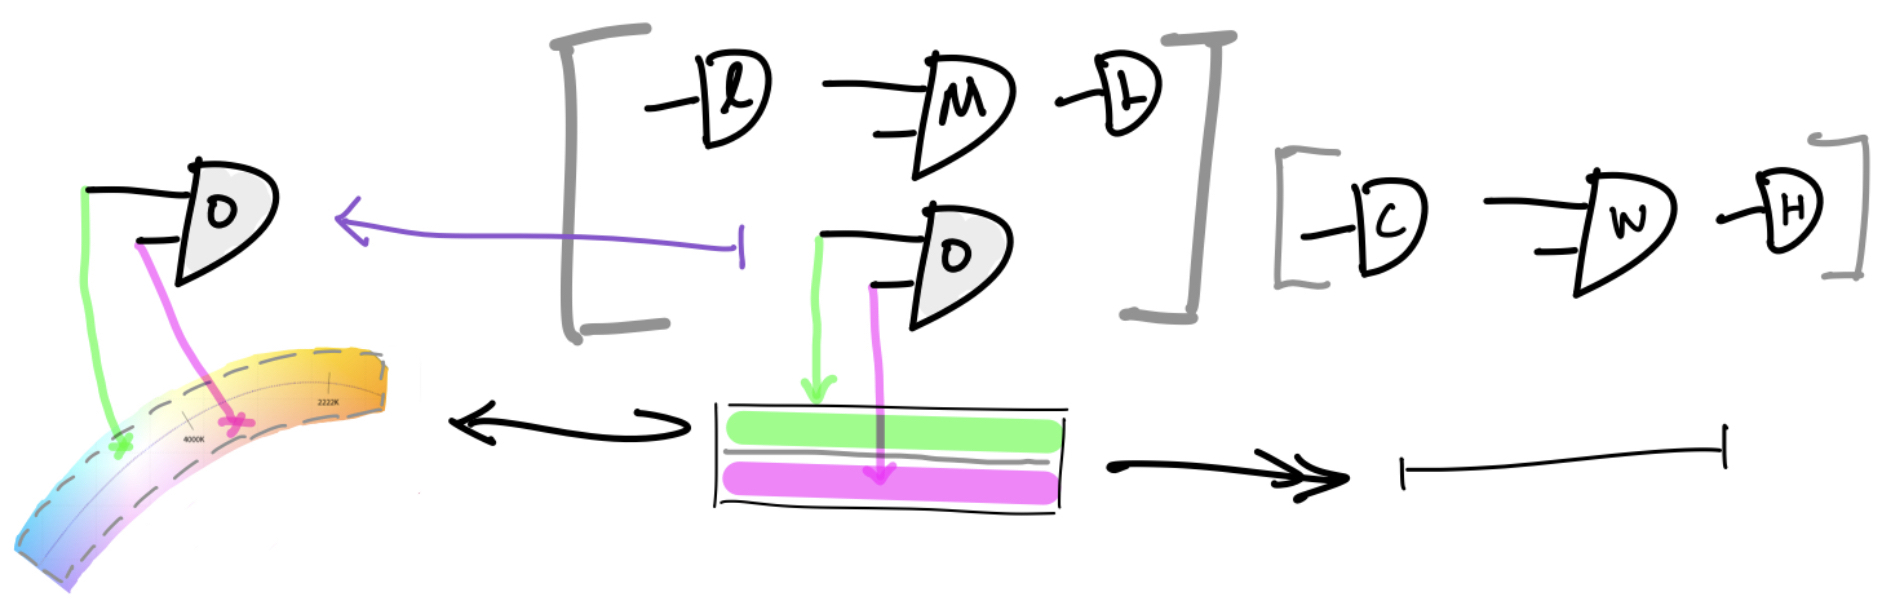
\includegraphics{figures/metaphor/offset2.jpeg}}
\caption{The additional expressive power that the apex strip gives is the concept of vertical offset, which doesn't appear in the real line. So the apex strip allows talk of quantity and offset, and this offset, when translated into the colour domain, allows talk of offset towards and away from, for instance, green.}
\end{figure}
\end{example}
\clearpage

\subsection{Time and Money: complex conceptual structure}

Metaphor is perhaps the only methodology we have for making sense of certain abstract concepts, such as Time. For example, many languages make use of the metaphor \texttt{TIME is SPACE}, in which space-talk is used to structure time. In English, the future is ahead of us and the past behind, while conversely, for the Aymara the future is behind and the past is ahead. Orthogonally, in Mandarin the future is below and the past is above. We have already demonstrated that we have the tools to deal with conceptual transfer between static conceptual spaces viewed as topological spaces via spans of continuous maps. What is of concern to us are \emph{dynamic} metaphors that involve a conceptual space-\emph{time} with agents and capabilities and so on. The following discussion draws heavily from \citep{lakoff_metaphors_2003}.\\

For example, in English, we make ample use\footnote{To our detriment. We could just as well have chosen the metaphor \texttt{TIME is FOOD}, which provides a liberating sense of mastery (at least in a context where food is abundant): time can be prepared, produced, consumed, spiced if dull and best shared with loved ones.} of the metaphor \texttt{TIME is MONEY}. There two mathematically relevant aspects of metaphor that I want to draw attention to for this metaphor. Firstly, that the conceptual affordances money-talk is marshalled to give structure to time-talk, where there is no such structure were it not for the metaphor. Secondly, that metaphor has a partial nature, in that it is not the case that the metaphor licenses all kinds of money-talk to structure time-talk.\\

To establish the first point of conceptual transfer, a phrase like \texttt{Do you have time to look at this?} is completely sensible to us, but literally meaningless; even if we had an oracle to measure possession, what would we point it at to measure a person's possession of time? Even if we accept some argument that the concept of possession is innate to the human faculty, when we say \texttt{This is definitely worth your time!} or \texttt{What a waste of time.}, we are drawing upon value-talk that is properly contingent in the socially constructed sense upon the conceptual complex of money.\\

To establish the second point of partiality, consider that money can be stored in a bank, whereas there is no real corresponding thing in the common conceptual vocabulary which one can store time and withdraw it for later use\footnote{Although, in a wonderful example of `pataphysical thinking, "Time Banks" have existed since the 19th century, which are practices of reciprocal service exchange that use units of time as currency.}. But the partiality constraint is itself partial. For instance, one can invest money into an enterprise in the expectation of greater returns, and this is not appropriate for many domains of time-talk, but there is a metaphorical match in some specific contexts, such as text-editor-talk: \texttt{learning vim slows you down at first but it will save you time later}.\\

Now I'll try to demonstrate by example that the kinda-cofunctors we explored in Section \ref{sec:miracle} between text circuits do all of the things we have asked for. The components of text circuits serve as an algebraic basis for dynamic conceptual complexes, while the kinda-cofunctor handles partial structuring of one conceptual domain in terms of another.

\begin{example}[\texttt{Vincent spends his morning writing}]
To begin a formal figurative interpretation via the metaphor \texttt{TIME is MONEY}, we require some model of the conceptual domain of money, as well as a topological interpretation. As a first pass, we understand that money can be exchanged for goods and services, so we will settle for a text-circuit signature for trade to serve as the conceptual domain as the apex of a cofunctor, given in Figure \ref{fig:tradesig}. The elements of the topological model are given in Figure \ref{fig:topmodel}. The behaviour of the opfibration part of the cofunctor is detailed in Figure \ref{fig:fibroles}, and that of the identity-on-objects functor in Figures \ref{fig:interpret}, \ref{fig:time0}, and \ref{fig:time1}. The figurative model serves as a foundation from which truth-theoretical semantics can begin. In the sketched interpretation, there aren't too many interesting questions one can ask, but the purpose of this example is to point out that in principle, we can exploit the systematicity of metaphor by constructing figurative mechanical models for which interesting questions can be asked and answered truth-theoretically, as in Figure \ref{fig:fullermodel}.
\begin{figure}[h]\label{fig:tradesig}
\centering
\resizebox{\textwidth}{!}{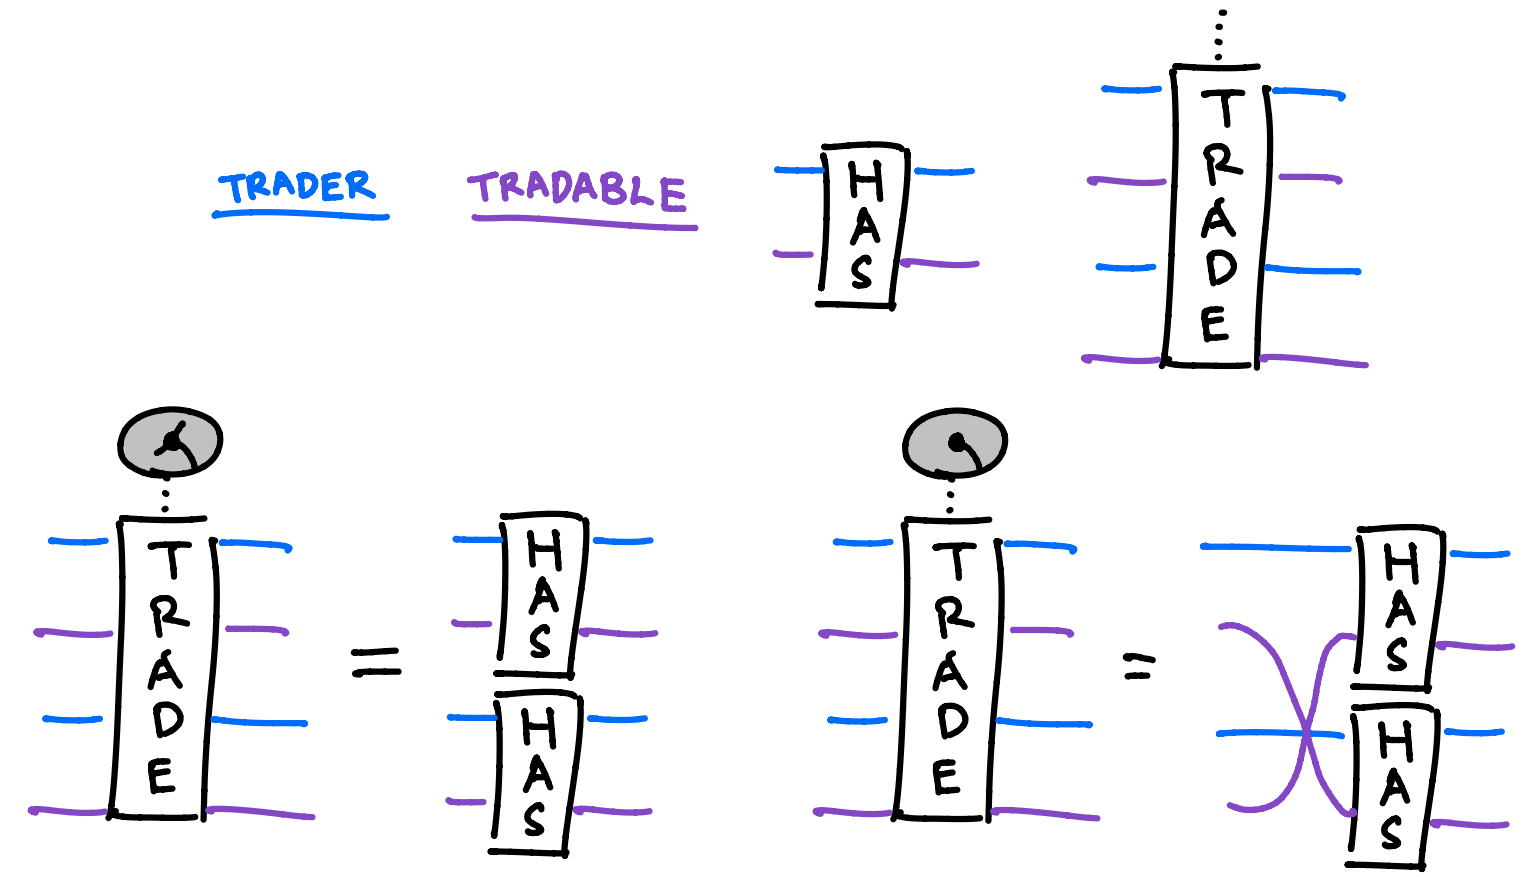
\includegraphics{figures/metaphor/tradesignature}}
\caption{In the \texttt{TRADE} signature, we define two roles as wires: \texttt{TRADERS} and \texttt{TRADEABLES}. There is one static relation \texttt{HAS} to indicate a trader's ownership of a tradeable, which can be further elaborated with equations to indicate e.g. exclusivity of ownership by interpreting violations of exclusivity as a zero morphism, assumed but elided for brevity. There is one dynamic verb (treated as a homotopy) \texttt{TRADE}, which at time 0 enforces a precondition that the traders have their respective tradables, and at time 1 (completion of the trade), the traders swap possession of their tradeables. The \texttt{TRADE} signature contains all nominal instantiations of nouns with respect to roles, which will be illustrated shortly.}
\end{figure}
\begin{figure}[h]\label{fig:topmodel}
\centering
\resizebox{0.75\textwidth}{!}{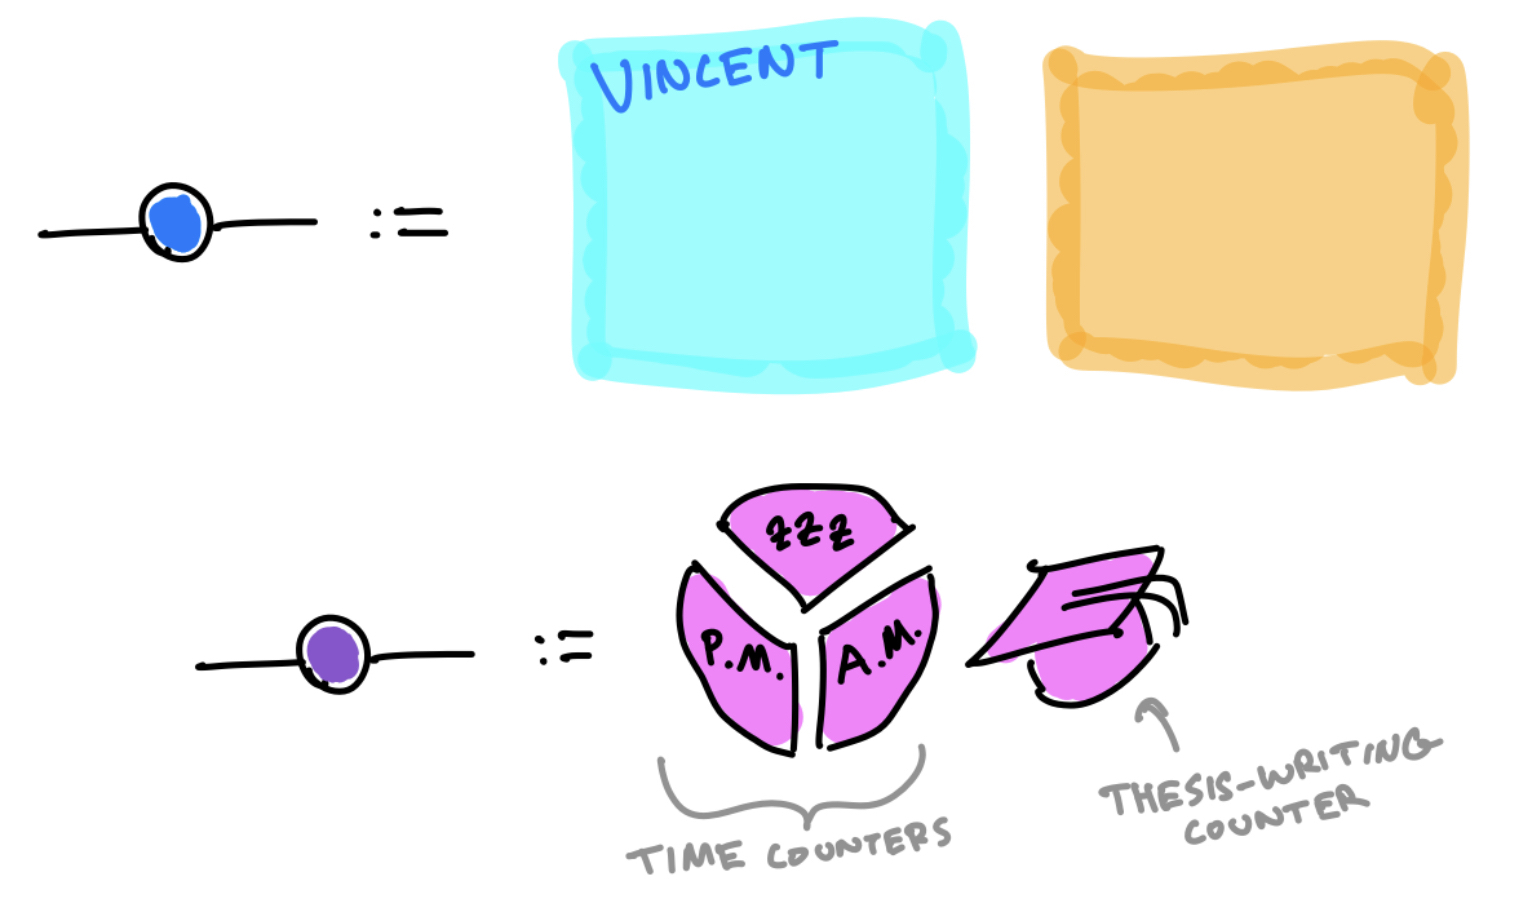
\includegraphics{figures/metaphor/toptrademodel.jpeg}}
\caption{We build the topological model from two sticky spiders in the Euclidean plane. The \texttt{TRADER} spider will distinguish two regions of possession, so that \texttt{HAS} may be interpreted as a region-test. The \texttt{TRADEABLES} spider will specify four meeples or counters, three for time, and one for thesiswriting; we will use the configuration space of the \texttt{TRADEABLES} spider to regulate their movement and distribution.}
\end{figure}
\begin{figure}\label{fig:fibroles}
\centering
\resizebox{\textwidth}{!}{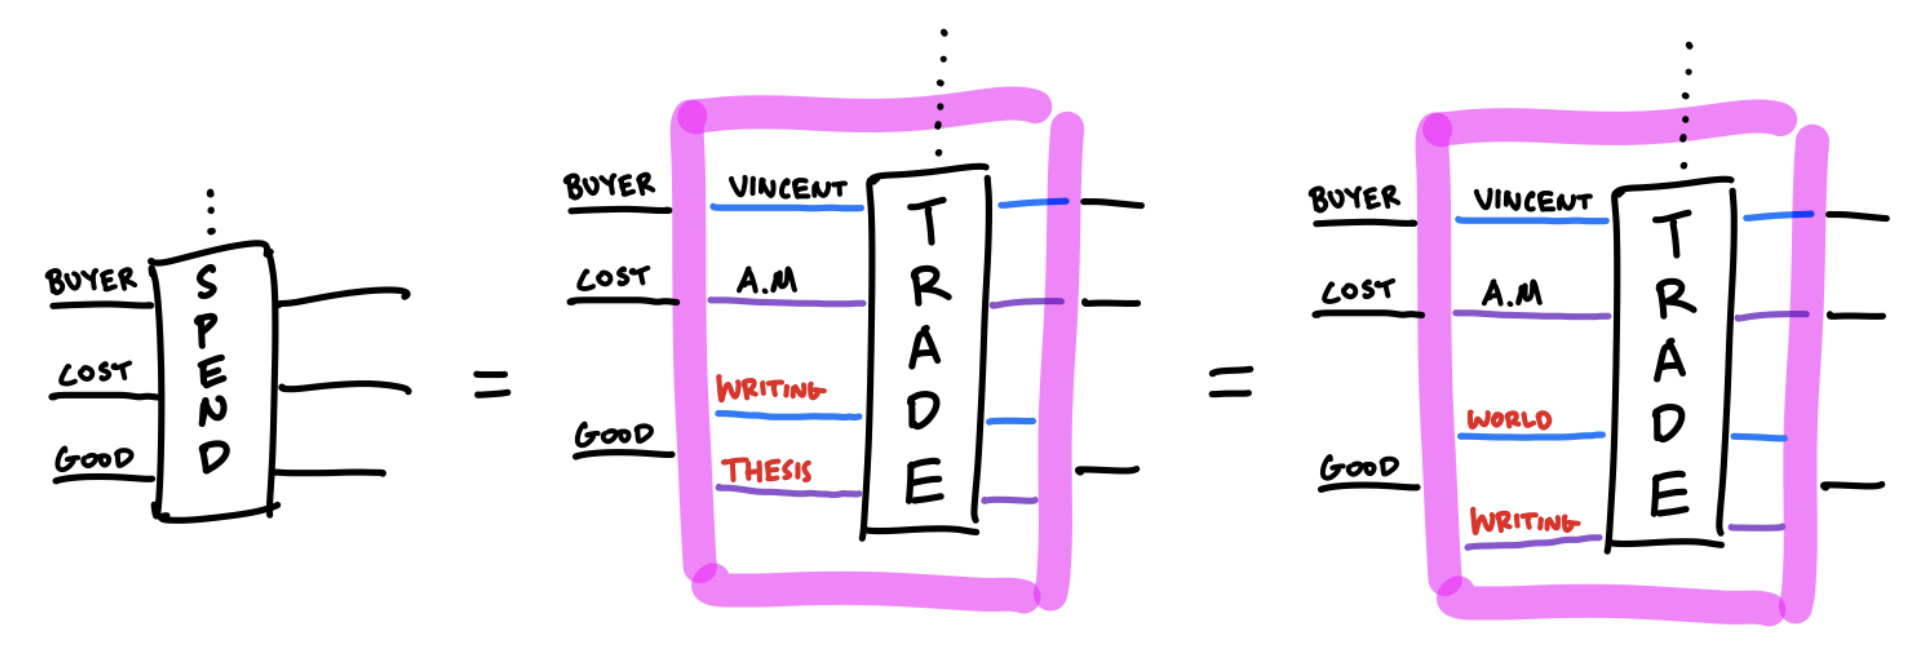
\includegraphics{figures/metaphor/fibroles}}
\caption[-10cm]{Next, we have to specify what the discrete opfibration is doing. Recalling our functor box notation, we can consider the job of the discrete opfibration to be role assignment from the verb \texttt{SPEND} in the utterance to the verb \texttt{TRADE} in the conceptual domain. The opfibration forgets about role-assignments in its domain by sending them to the monoidal unit. The lift of the opfibration is a role-assignment. (Arguably) unambiguously in this example, \texttt{Vincent} is the spender and the first trader, and \texttt{A.M} is the cost and the first tradeable. However, there are two options to resolve \texttt{writing} treated as a noun-phrase in the role of \texttt{GOOD}. In the first lift, \texttt{writing} is resolved as the other trader, and the implicit good as \texttt{thesis}. In the second lift, \texttt{writing} is the tradeable and something else is the trading counterparty, such as \texttt{the world}.}
\end{figure}
\begin{figure}[h]\label{fig:interpret}
\centering
\resizebox{0.5\textwidth}{!}{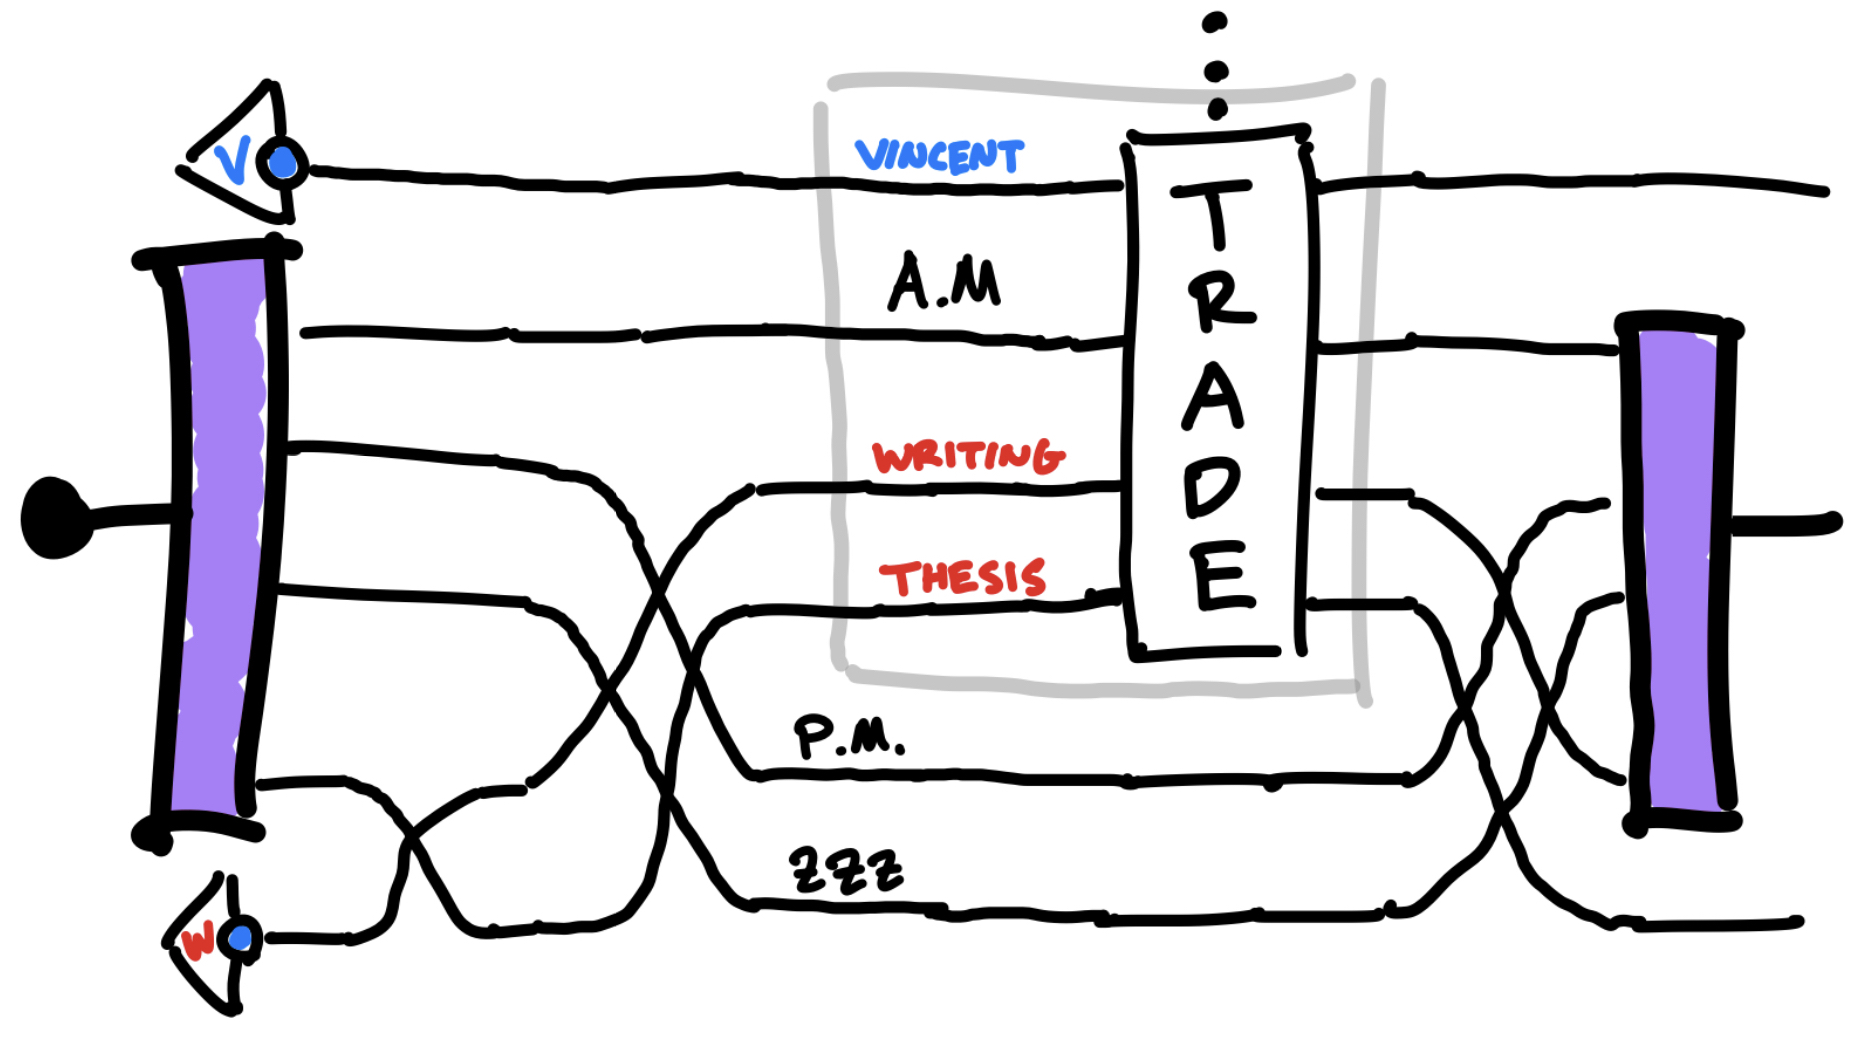
\includegraphics{figures/metaphor/interpret.jpeg}}
\caption{The section of the opfibration over the \texttt{SPEND} verb is a tabulation of all the ways in which conceptual roles in the \texttt{TRADING} domain can be assigned. To continue the example, we will assume the first lift in Example \ref{fig:fibroles} as our interpretation. The identity-on-objects functor part of the cofunctor maps our chosen interpretation into the following diagram in \textbf{ContRel}. The configuration space of the \texttt{TRADEABLES} spider is expanded via split idempotent so that all thin wires in the diagram are typed as the Euclidean plane. Recalling Example \ref{ex:chessboard}, \texttt{HAS} is interpreted as the intersection of the position of a counter with the possessive region of the respective trader.}
\end{figure}
\begin{figure}[h]\label{fig:time0}
\centering
\resizebox{\textwidth}{!}{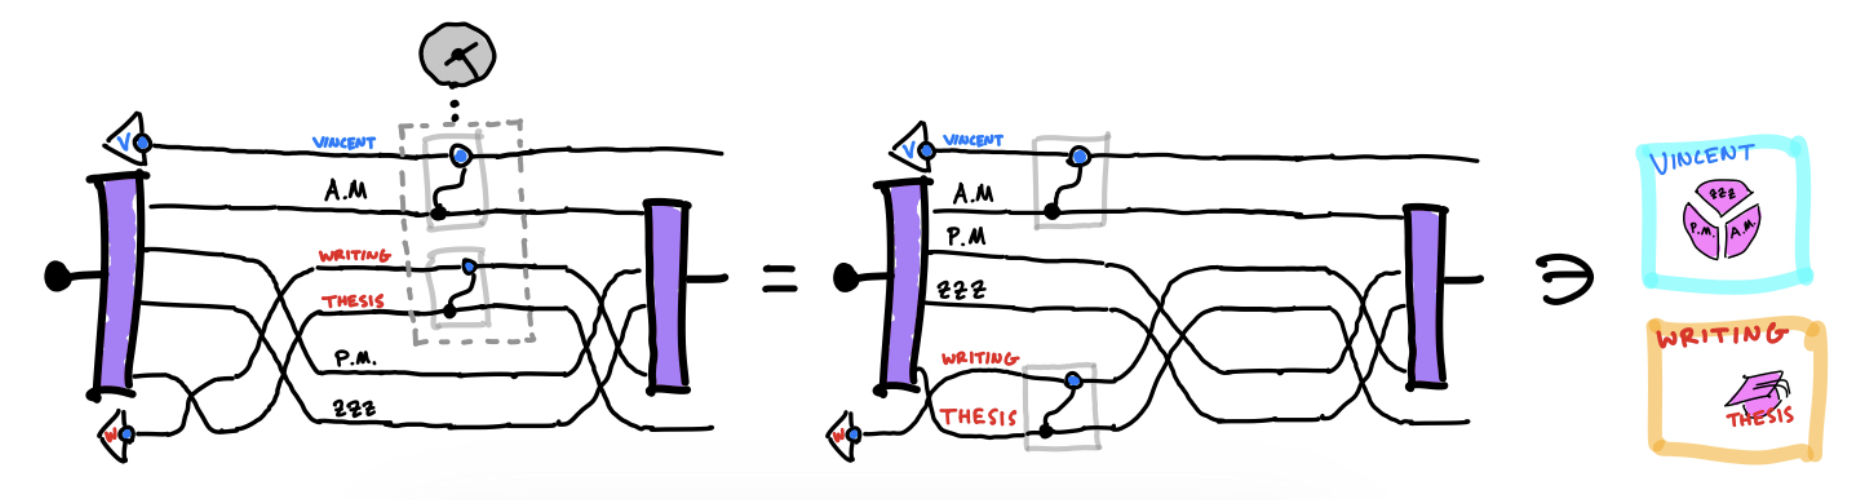
\includegraphics{figures/metaphor/time0.jpeg}}
\vspace{5cm}
\caption{We may verify that the equations governing \texttt{TRADE} cohere with our topological figures. At time 0, before the trade, we can calculate that the permissible figures have \texttt{Vincent} in possession of \texttt{A.M} and \texttt{writing} in possession of \texttt{thesis}.}
\end{figure}
\begin{figure}[h]\label{fig:time1}
\centering
\resizebox{\textwidth}{!}{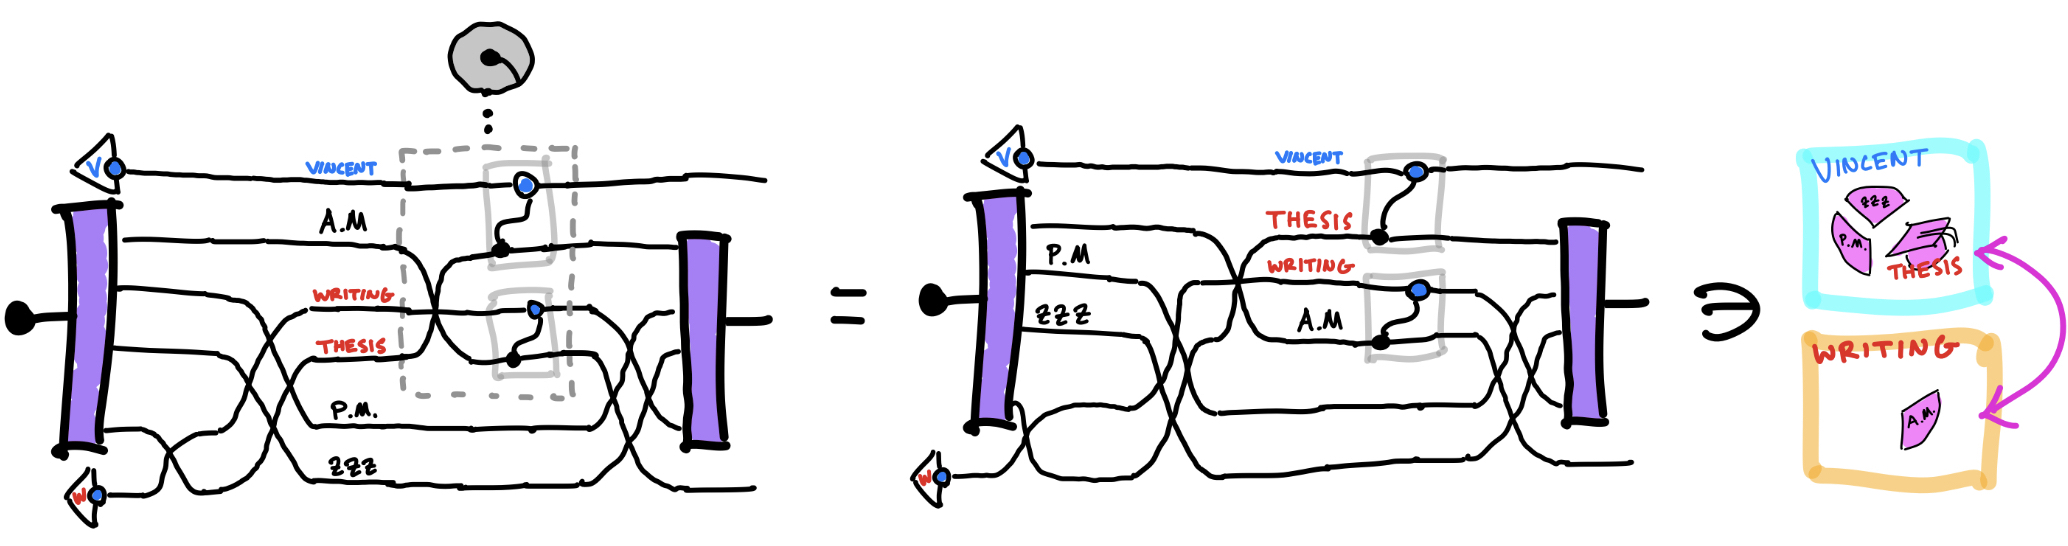
\includegraphics{figures/metaphor/time1.jpeg}}
\caption{At time 1, we may calculate that the permissible figures must be such that \texttt{Vincent} is in possession of \texttt{thesis} and \texttt{writing} is in possession of what was previously my morning.}
\end{figure}
\begin{figure}[h]\label{fig:fullermodel}
\centering
\resizebox{\textwidth}{!}{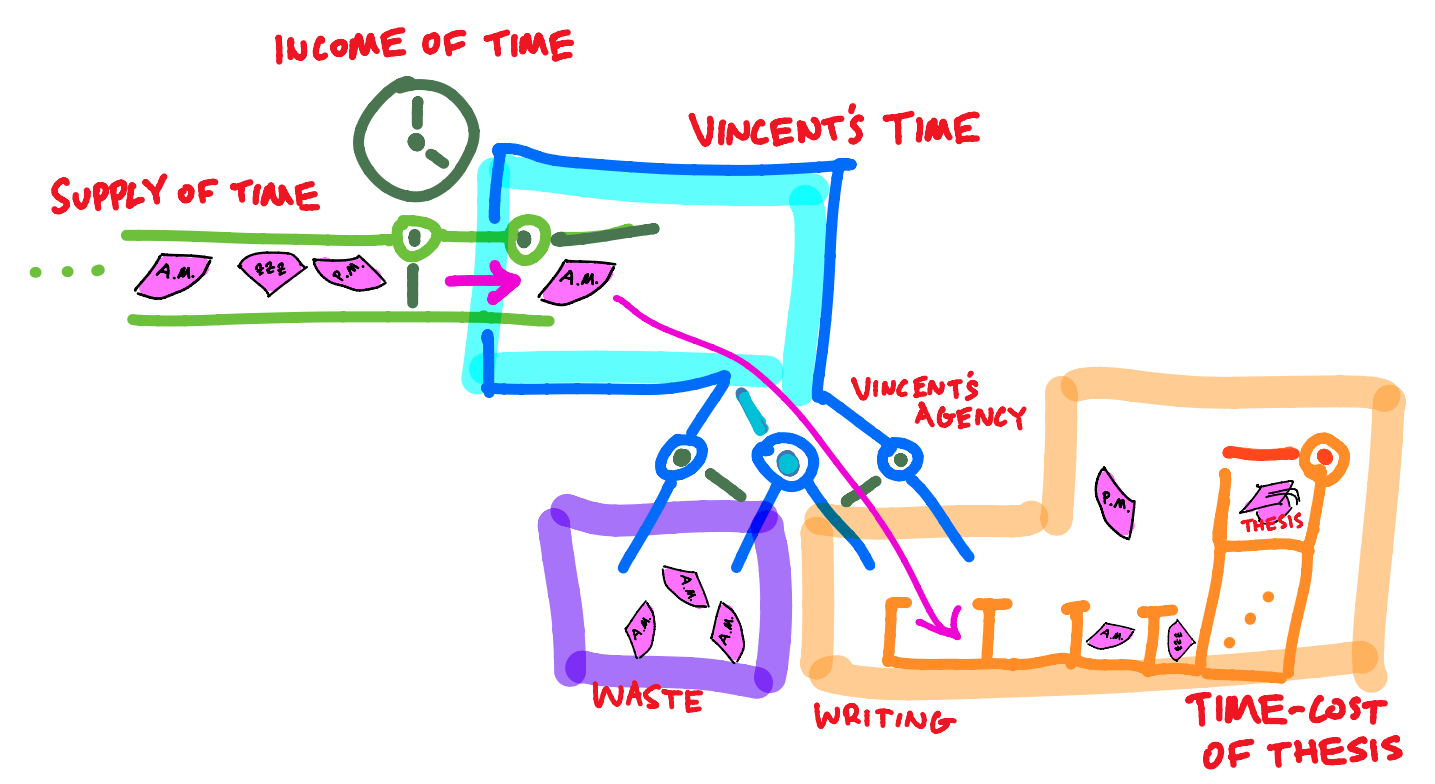
\includegraphics{figures/metaphor/fullermodel}}
\caption{In a more detailed conceptual model of \texttt{TIME is MONEY}, rather than just \texttt{TRADE}, we might consider income, the spender's agency, and cost. In Euclidean 3-space, we might model income as a clock-gated mechanism that deposits time-tokens serially into Vincent's possession, along with his agency as a gated chute, and the time cost of writing a thesis as a dispenser that requires a certain number of tokens to release a thesis-token into Vincent's possession. In this sketch model, one obtains short films for \texttt{He used to waste his mornings but now he spends them writing}, or \texttt{He once spent an evening writing but made no progress}. One can then ascertain certain consequences truth-theoretically; for instance that there is at least one morning that was not spent on writing, or that there is at least one evening spent on writing but not inside the slot that would help a thesis-release mechanism trigger. In every case, cofunctoriality handles bookkeeping for role-interpretation choices and guarantees systematicity of the topological figure according to the signature at the apex model that models the organising concept.}
\end{figure}
\end{example}

\clearpage

\clearpage
\newpage

\newthought{\textbf{Objection:} Hold on, that last figure wasn't justified.} It's justified in principle.

\newthought{\textbf{Objection:} On what principles?} Good question!

\section{The logical conclusions}

Like how the Church-Turing thesis is a declaration of the limits of computability by informed consensus, we might ask what idealised theses we might posit. Now we recap what we've seen.

\newthought{Review of Chapter 1.} We demonstrated that by encoding meaning-relations as topological connectivity (which is in a broad sense the whole point of string diagrams as a bridge between algebra and topology), we can capture systematic structural relationships as configurations of functors. In particular, we were able to diagrammatically reason about the correspondence between a pair of simple productive and parsing grammars subject to the evident constraints of communication. With some imagination, there are two theses here to obtain, or declare:

\begin{thesis}[String diagrams for composition]
Compositionality equals topological representability; in particular, meaning relations in text are witnessed by connectivity of string diagrams.
\end{thesis}

\begin{thesis}[String diagrams for systematic relationships]
Systematicity equals functorially witnessed relations; in particular, spans of functors between families of string diagrams witness agreement between different theories as topological equivalence.
\end{thesis}

\newthought{Review of Chapter 2.} We demonstrated that from the  mathematical perspective of weak $n$-categories, there is no fundamental difference between a broad class of productive grammars at a structural level, including all string-rewrite systems, tree-adjoining grammars, and transformational grammars. In this setting, we created a circuit-growing grammar and demonstrated a correspondence -- the Text Circuit Theorem -- between text circuits and grammatical text for a fragment of English, hence justifying the na\"{i}ve composition of text circuits as a generative grammar. We moreover indicated how the correspondence could be expanded to cover larger fragments of English, and indicated how the particular form of text circuits made them preferable for practical application. We also mentioned that in some sense the correspondence wasn't important from the perspective that text circuits were algebraic jazz for text. Putting together the views from Chapters 0, 1 and 2, productive grammars are just ways of generating topological data, and the only practically interesting constraint about whether a productive grammar is suitable for natural language stems from whether it is paired with a parsing grammar that systematically agrees on semantics up to topological equivalence -- i.e. precisely the kind of equivalence that string diagrams are invariant under. So we might reach for:

\begin{thesis}[String diagrams for syntax]
Syntax equals a coherent method of synthesising \emph{and} analysing composition; in particular, any internally consistent conception of natural language syntax in terms of string diagrams is permissible.
\end{thesis}

\newthought{Review of Chapter 3.} We give content to string diagrams by interpreting them in the category of continuous relations \textbf{ContRel}. We string-diagrammatically characterised labelled collections of disjoint shapes, along with processes that allowed us to puppeteer them in space, and test for topological relationships between shapes and places such as containment and touching. In particular, since we defined rigid motions and spatial-exclusivity of shapes, we have covered enough to linguistically specify any mechanical model up to topological invariance, and it is no difficulty to see how this setting may be expanded to include distances, directions, and forces. We saw how \textbf{ContRel} naturally gives voice to the structure of text circuits as higher-order modifications, and we also saw how \textbf{ContRel} permits us to model simple intensions via containers that mirror the space around them, which also yields a novel mathematical model of \textbf{FinRel} equipped with a Turing object, which is a mathematical model for universal computation and, in the linguistic setting, syntactic polymorphism. On the faith that any consistent and interesting system of string diagrams has some consistent and interesting computational reification, we might integrate the views of the previous chapters to obtain:

\begin{thesis}[String diagrams for semantics]
Semantics equals computatation; in particular, any consistent computational interpretation of the content of string diagrams is permissible.
\end{thesis}

\subsection{How things could be.}

\begin{thesis}[String diagrams for text]
String diagrams suffice for formal linguistics.
\end{thesis}

That's the best-case scenario if we accept all of the best-case scenarios above. What would such a hypothetical world look like? Recall that I still owe a worked example of computing a metaphor. Sadly, I think in a best-case hypothetical world, working out the conduit metaphor would be a kind of dull problem sheet for undergraduate mathematical linguists, who may well ask "what's the point?". Indeed, what is the point of learning all of this mathematically complicated machinery to do something everyone can do effortlessly? I'm not sure of the answer, but I do know that turning language into pictures by turning language into pictures was good fun.

\newpage

\includepdf[angle=90,pages=-]{metaphorproblemsheet-filled}

\bibliographystyle{alpha}
\bibliography{thesis_intro}

\end{document}